%%%%%%%%%%%%
%% Please rename this main.tex file and the output PDF to
%% [lastname_firstname_graduationyear]
%% before submission.
%%
%% This .tex file is for use with BibLaTeX. Please use
%% main-bibtex.tex instead if you prefer BibTeX.
%%%%%%%%%%%%

\documentclass[12pt]{caltech_thesis}
\usepackage[hyphens]{url}
\usepackage{lipsum}
\usepackage{graphicx}

%Zach's packages and commands
\usepackage{braket}
\usepackage{caption}
\usepackage{subcaption}
%\usepackage{subfigure}

\DeclareOldFontCommand{\rm}{\normalfont\rmfamily}{\mathrm}
\DeclareOldFontCommand{\it}{\normalfont\itshape}{\mathit}

%%Matt's packages and commands

\newcommand{\note}[1]{\textcolor{blue}{[#1]}}

%% added for gcbh chapter
\usepackage{amsmath}
\usepackage{amssymb}
\usepackage{multicol}
\usepackage{bm}
\usepackage{pdflscape}
\usepackage[T1]{fontenc}
\usepackage{ae,aecompl}

%% added for high spins
\usepackage{xspace}
\usepackage[usenames,dvipsnames]{color}
\usepackage{mathrsfs}

%% added for overtones
\usepackage{microtype}
\usepackage{etoolbox}

\newcommand{\xten}[1]{\times 10^{#1}}
\newcommand{\sub}[1]{_{\mathrm{#1}}}
\newcommand{\map}[1]{\ensuremath{\mathcal{M}_{\mathrm{#1}}}}
\newcommand{\distorted}[1]{\hat{#1}}
\newcommand{\inertial}[1]{\bar{#1}}
\newcommand{\newgrid}[1]{\breve{#1}}
\newcommand{\newdistorted}[1]{\grave{#1}}
\newcommand{\grid}[1]{#1}
\newcommand{\spin}[1]{\ensuremath{S^{++}_{0.{#1}}}\xspace}
\newcommand{\generic}{\ensuremath{S^{0.99}_{0.20}}\xspace}
\newcommand{\roughly}{\mathchar"5218\relax} % Different from \sim in spacing

%% added to template (MG)
\usepackage[dvipsnames, usenames]{xcolor}
\definecolor{linkcolor}{rgb}{0.0,0.3,0.5}
\usepackage[hypertexnames=false, unicode, colorlinks=true, linkcolor=linkcolor, citecolor=linkcolor, filecolor=linkcolor,urlcolor=linkcolor, pdfusetitle]{hyperref}
\usepackage[all]{hypcap}


\usepackage{todonotes}

%% newtx for better-looking Times
\usepackage[utf8]{inputenc}
\usepackage[T1]{fontenc}
\usepackage{newtxtext,newtxmath}


%%%% add deeper TOC numbering and deeper inclusion
\setcounter{tocdepth}{2}
\setcounter{secnumdepth}{4}

% Must use biblatex to produce the Published Contents and Contributions, per-chapter bibliography (if desired), etc.
\usepackage[
    backend=biber,natbib,
    % IMPORTANT: load a style suitable for your discipline
    style=numeric-comp,
    sorting=none
]{biblatex}


\def\aj{\textrm{AJ}}
\def\apj{\textrm{ApJ}}
\def\apjl{\textrm{ApJ}}
\def\apjs{\textrm{ApJS}}
\def\aap{\textrm{A\&A}}
\def\aaps{\textrm{A\&AS}}
\def\mnras{\textrm{MNRAS}}
\def\prd{\textrm{PRD}}
\def\prl{\textrm{PRL}}
\def\prx{\textrm{PRX}}
\def\nat{\textrm{Nature}}
\def\cqg{\textrm{CQG}}
\def\grg{\textrm{GRG}}
\def\lrr{\textrm{LRR}}
%%
\def\ssr{\textrm{Space Sci. Rev.}}
\def\bain{\textrm{Bull. Astron. Inst. Netherlands}}
\def\apss{\textrm{Ap\&SS}}
\def\aapr{\textrm{A\&A Rev.}}
\def\pasj{\textrm{PASJ}}



% Name of your .bib file(s)
\addbibresource{ownpubs.bib}
\addbibresource{references.bib}

\begin{document}

\title{Gravitational Wave Signatures of Black Hole Physics}
\author{Zachary Mark}


\degreeaward{Doctor of Philosophy}                 % Degree to be awarded
\university{California Institute of Technology}    % Institution name
\address{Pasadena, California}                     % Institution address
\unilogo{caltech.png}                                 % Institution logo
\copyyear{2021}  % Year (of graduation) on diploma
\defenddate{December 4, 2020}          % Date of defense
\orcid{0000-0003-2300-893X}


%% IMPORTANT: Select ONE of the rights statement below.
\rightsstatement{All rights reserved}
% \rightsstatement{All rights reserved except where otherwise noted}
% \rightsstatement{Some rights reserved. This thesis is distributed under a [name license, e.g., ``Creative Commons Attribution-NonCommercial-ShareAlike License'']}

%%  If you'd like to remove the Caltech logo from your title page, simply remove the "[logo]" text from the maketitle command
\maketitle[logo]
%\maketitle

%% acknowledgements
\begin{acknowledgements} 	 
  I could not have made it here without the unwavering support of my advisor Yanbei Chen. He helped me navigate the world of gravitational physics and stuck with me when I explored new topics. More importantly, he was interested in not only my success as a researcher but also my happiness as a person.

I also owe a huge thanks to Rana Adihikari, who inspired new research directions later in my PhD. I would not have been able to finish this thesis without his mentorship and patience. 

I greatly appreciate the guidance that I received from the rest of my committee, Saul Teukolsky, who frequently answered my many questions throughout my degree, and Yaser Abu-Mostafa, who joined my committee even though it was outside of his research interests.

I'm extremely grateful to the prior generation of TAPIR graduate students, especially Huan Yang, Aaron Zimmerman, and my undergraduate advisor Rob Owen. Huan, Aaron, and Rob all invested a significant amount of time and energy in my development as a physicist. 

I'm thankful that I worked with and learned from many brilliant and altruistic people at Caltech, including but not limited to: Chad Galley, Matthew Glieser (a special thanks for the thesis template help), Kevin Barkett, JoAnn Boyd, Craig Cahillane, Boayi Chen, Bassam Helou, Max Isi, Kevin Kuns, Yichu Ma, Morgan Nanez, David Nichols, Masha Okonouva, Belinda Pang, Mark Scheel, Leo Stein, Anandh Swaminathan, Ron Tso, Vija Varma, Hang Yu (a special thanks for helping me learn the background for the noise regression work)

And obviously a huge thanks to my mom, dad, and siblings Ian, Melissa, and Allie, as well as all of my friends.



\end{acknowledgements}

%% abstract
\begin{abstract}
WRITE ABSTRACT
  
\end{abstract}

%% Uncomment the `iknowhattodo' option to dismiss the instruction in the PDF.
\begin{publishedcontent}[iknowwhattodo]
% List your publications and contributions here.
  \nocite{Scheel:2014ina,Giesler:2017uyu,Giesler:2019uxc,Isi:2019aib,
    Lovelace:2014twa,Bhagwat:2017tkm}
\end{publishedcontent}


\tableofcontents
\listoffigures
\listoftables
\printnomenclature

\mainmatter

%%%% comment/uncomment to include chapter in compilation
%\begin{refsection}
\newcommand{\LL}{\mathcal{L}}
\newcommand{\DD}{\mathcal{D}}
\def\p{\bar{\rho}}


\chapter{The Quasinormal Modes of Weakly Charged Kerr-Newman Spacetimes}
\label{chap:KN_QNM}

\begin{centering}
Zachary Mark, Huan Yang, Aaron Zimmerman, and Yanbei Chen \\
Phys. Rev. D 91, 044025 (2015) \\
\href{https://https://arxiv.org/abs/1409.5800}{arxiv:1409.5800} \\
\end{centering}

\section{Abstract}
The resonant mode spectrum of the Kerr-Newman spacetime is presently unknown.
These modes, called the quasinormal modes, play a central role in determining the stability of Kerr-Newman black holes and their response to perturbations.
We present a new formalism, generalized from time-independent perturbation theory in quantum mechanics, for calculating the quasinormal mode frequencies of weakly charged Kerr-Newman spacetimes of arbitrary spin. 
Our method makes use of an original technique for applying perturbation theory to zeroth-order solutions that are not square-integrable, and it can be applied to other problems in theoretical physics. 
The new formalism reveals no unstable modes, which together with previous results in the slow-rotation limit strongly indicates the modal stability of the Kerr-Newman spacetime. 
Our techniques and results are of interest in the areas of holographic duality, foundational problems in General Relativity, and possibly in astrophysical systems.


\section{Introduction}
 
The resonant modes of a perturbed black hole spacetime are called quasinormal modes (QNMs) \cite{Berti2009}. They are found by solving an eigenvalue problem, similar to the type encountered in quantum mechanics, that arises from linearizing the Einstein-Maxwell (EM) equations about a stationary black hole background. The most general, stationary black hole solution in EM theory is the Kerr-Newman (KN) spacetime, which possesses a mass $M$, a specific angular momentum $a$, and an electric charge $Q$. The calculation of the QNM frequency spectrum of the perturbed KN spacetime is a major unsolved problem in General Relativity~\cite{ChandraBook}.

The KN QNM spectrum is a key component in a variety of problems involving charged black holes. Astrophysical black holes may temporarily acquire charge during compact binary mergers, as there could be nonzero charge distribution in their surrounding plasma~\cite{Alic2012,Lehner2012}, although in the stationary limit charges tend to be neutralized due to vacuum polarization~\cite{Gibbons75}. 
Computing the QNM frequencies is the first step in addressing the stability of the KN spacetime to perturbations, which remains an open question.
Knowledge of the KN QNMs would also assist efforts to determine whether the self force acts as a ``cosmic censor'' that prevents a KN black hole from being overcharged ($Q>Q_\text{max}=\sqrt{M^2-a^2}$) when a charged particle crosses the horizon~\cite{ZimmermanPoisson}. To determine the self force, the joint evolution of gravitational and electromagnetic fields induced by the motion of the charged particle 
must be evaluated consistently, a difficulty which may be amenable to the techniques we use here.
Studies of KN QNMs may be also relevant for string theory and holographic dualities~\cite{Berti2009}. In particular, according to the AdS/CFT correspondence~\cite{Maldacena:1997re}, the QNM spectrum of the bulk spacetime coincides with poles of the Green function of the boundary gauge theory. Extension of this work to KN-AdS~\cite{Caldarelli:1999xj} black holes can help to understand charged conformal fields on the boundary.

Current techniques to calculate QNM frequencies, such as Leaver's continued fraction method \cite{Leaver1985}, numerical shooting methods \cite{PressTeukolsky1973}, and newer techniques~\cite{Pani2013PHYSD,Pani:2013pma} require that the linearized EM equations separate.
The study of perturbations to both the charged, non-rotating Reissner-Nordstr\"{o}m (RN) black hole, and the rotating Kerr black hole can be reduced to the study of separable, decoupled wave equations, known as  the Zerilli-Moncrief~\cite{Zerilli1974,Moncrief1974odd,Moncrief1974even} and Teukolsky equations~\cite{Teukolsky1973,PressTeukolsky1973,TeukolskyPress1974}, respectively. 

The problem of arriving at separable, decoupled equations governing gravitational and electromagnetic perturbations to the charged, rotating KN black hole is considerably harder. There is not enough symmetry to facilitate separation a priori, and the background electric field introduces interactions between the gravitational and electromagnetic perturbations which make decoupling nontrivial. 
Pani, Berti, and Gualtieri~\cite{Pani2013PRl,Pani2013PHYSD} dealt with these issues by working in the slow-rotation limit, where they found that the linearized KN equations separate and can be reduced to a pair of coupled ordinary differential equations. 
They were able to extract the QNM frequency spectrum using a matrix-valued version of Leaver's continued fraction method and their analysis revealed no unstable modes. 
Dudley and Finley derived a wave equation (hereafter referred to as the DF equation) that is exact for scalar perturbations, but is a conceptually questionable approximation for gravitational and electromagnetic modes~\cite{Dudley:1977zz,Dudley1979}.
Berti and Kokkotas \cite{BertiKokkotas2005} conjectured that the DF equation is accurate for weakly-charged KN spacetimes by comparing its predictions for RN black holes to those from the Zerilli-Moncrief equation. 

In this paper we provide a new formalism, which we refer to as the eigenvalue perturbation (EVP) method, that is accurate to first order in $q\equiv Q^2/M^2$ and can be potentially extended to arbitrarily high orders in $q$. Our results show that the DF equation does not predict QNM frequencies that are accurate to first order in $q$, except for a special set of modes of rapidly rotating black holes. Our first order calculations in $q$ reveal no unstable modes, which, when complemented by the slow rotation study~\cite{Pani2013PRl,Pani2013PHYSD}, provides strong evidence for the linear stability of the KN spacetime. In addition, we provide the first analysis of the nearly extremal Kerr-Newman (NEKN) QNM frequencies in the rapidly rotating regime. The EVP method makes use of an original technique for applying perturbation theory to zeroth order solutions which are not square-integrable. This method can be (and recently has been \cite{Zimmerman:2014aha,Yang:2014zva,Yang:2014tla}) applied to other problems in theoretical physics.

\section{QNM frequencies of weakly charged black holes}

Following the derivation of the Teukolsky equation, we work in the Newman-Penrose (NP) formalism~\cite{NewmanPenrose1962,ChandraBook,StewartBook}, where the fundamental equations of general relativity are projected onto a null tetrad. 
In the NP formalism, spin-weighted fields $\psi_s$ capture the information about the gravitational ($s=\pm 2$) and electromagnetic ($s =\pm 1$) perturbations. The spin-weighted fields are defined in terms of the Weyl scalars (for $s = \pm 1, \pm 2$) and are further discussed in the Appendix. 

\subsection{The coupled equations} 

We begin with the coupled equations for the scalars $\psi_1$ and $\psi_2$. Following Chandrasekhar \cite{ChandraBook}, we expand all NP quantities in frequency and azimuthal harmonics $e^{-i\omega t+im\phi}$, with harmonic indices implicit. Using similar steps as those used to derive the Teukolsky equation, we reduce the EM equations to two coupled equations governing the gravitational and electromagnetic degrees of freedom, which can schematically be written  
\begin{equation}
\begin{bmatrix}
\mathcal{H}_2 & q\delta \mathcal{H}_2 \\ \\
q \delta \mathcal{H}_1 &  \mathcal{H}_1 
\end{bmatrix}
\begin{bmatrix}
\psi_2 \\
\psi_1
\end{bmatrix}
=0.
\label{fun}
\end{equation}
The second order differential operators $\mathcal{H}_s$ and $\delta \mathcal{H}_s$, with $s =1,\,2$, contain derivatives in both $r$ and $\theta$. Their explicit form, as well as an outline of their derivation, is presented in~\cite{ChandraBook} and the Appendix. In all of the operators, the charge $Q$ only appears in the form $q = Q^2/M^2$, consistent with intuition that the frequencies cannot depend on the sign of the charge.
The $\delta \mathcal{H}_s$ operators are $\mathcal{O}(1)$ as $q \to 0$ [so the coupling terms are $\mathcal{O}(q)$] and Eq.~\eqref{fun} reduces to the $s=2$ and $s=1$ Teukolsky equations when $q \to 0$. The $\mathcal{H}_s$ operators differ from the unseparated, spin-weighted DF operator, which we denote by
$\mathcal{F}_s$, by an $\mathcal{O}(q)$ operator. This is why DF approximation fails to generate the correct order $\mathcal{O}(q)$ KN QNM frequencies. 

We are interested in the free oscillations of the KN spacetime, hence we supplement Eq.~\eqref{fun} with radiative boundary conditions; this means that we impose an ingoing boundary condition at the horizon and an outgoing boundary condition at spatial infinity. This turns  Eq.~\eqref{fun} into an eigenvalue problem for the QNM frequency $\omega =\omega_R -i\omega_I$. A positive $\omega_I$ indicates a decaying, stable mode and a negative $\omega_I$ indicates a growing, unstable mode.
Similar coupled equations can be derived for the perturbations to the Weyl scalars $\psi_{-1}$ and $\psi_{-2}$; though we are not yet able to demonstrate it, we believe that as in Kerr, they yield the same QNM frequency spectrum. 

\subsection{Perturbative formalism} 
We now calculate the QNM frequencies to $\mathcal{O}(q)$, which is the leading order correction to the frequency due the spacetime's charge. A solution to Eq.~\eqref{fun} consists of a frequency $\omega$, and a pair of spin-weighted fields $\psi_1$ and $\psi_2$ that satisfy the radiative boundary conditions. We expand our desired solution as a power series in $q$ around a QNM solution of Kerr,
\begin{align}
\psi_1 &= \psi_1^{(0)}+ q\psi_1^{(1)}+\mathcal{O}(q^2) \ , \nonumber\\ 
\psi_2 &= \psi_2^{(0)}+ q\psi_2^{(1)}+\mathcal{O}(q^2) \ , \nonumber\\ 
\omega &= \omega^{(0)}+ q\omega^{(1)}+\mathcal{O}(q^2) \ . \label{exp}
\end{align}
Either $\psi_1^{(0)}$ or $\psi_2^{(0)}$ are zero, since Eq.~\eqref{fun} decouples when $q=0$. Considering the gravitational perturbations first ($\psi_1^{(0)} = 0$) and plugging the expansions~\eqref{exp} into Eq.~\eqref{fun}, it is clear that the coupling terms enter at $\mathcal{O}(q^2)$ and can be neglected in our analysis. Expanding the $\mathcal{H}_s$ operators as a series in $q$, we obtain two decoupled equations for $\psi_2^{(1)}$ and $\psi_1^{(1)}$,
\begin{align}
&\mathcal{H}_2 \psi_2^{(1)} + \frac{\partial \mathcal{H}_2}{\partial q} \psi_2^{(0)}+ \omega^{(1)}\frac{\partial \mathcal{H}_2}{\partial \omega} \psi_2^{(0)} =0 \label{qmain}\,, \\
&\delta \mathcal{H}_1 \psi_2^{(0)}+ \mathcal{H}_1 \psi_1^{(1)}=0\,.
\end{align}
In the above expressions, we evaluate all operators at $q=0$ and $\omega = \omega^{(0)}$.

Equations of the form of Eq.~\eqref{qmain} are often encountered in quantum mechanics when we wish to calculate the corrections to the energy levels due to a small perturbing Hamiltonian. 
If we imagine that we likewise can define a finite product $\Braket{|}$ that makes the Teukolsky operator self-adjoint, meaning that $\Braket{\psi_s^{(0)} | \mathcal{H}_s \psi_s^{(1)} } = \Braket{\mathcal{H}_s \psi_s^{(0)} | \psi_s^{(1)} }= 0$ (with $\mathcal{H}_s$ again evaluated at $q =0$ and $\omega=\omega^{(0)}$),
we can derive a formula for $\omega^{(1)}$ by acting $\Bra{\psi_2^{(0)}}$ on both sides of  Eq.~\eqref{qmain}:
\begin{align} 
\omega^{(1)}=-\left .\Braket{\psi_2^{(0)}|\frac{\partial \mathcal{H}_2 }{\partial q}\psi_2^{(0)}} \right /\Braket{\psi_2^{(0)}|\frac{\partial \mathcal{H}_2 }{\partial \omega}\psi_2^{(0)}}\,.
\label{freqform}
\end{align}
An identical expression for the frequency correction to the electromagnetic QNM frequencies can be obtained from the same analysis with the $s=2$ subscript replaced by $s=1$. 
However, the stable Kerr QNM wave functions ($\omega_I < 0$) are not square-integrable along the real $r$-axis, since the radiative boundary conditions cause them to diverge at 
\begin{align}
&\psi_s^{(0)} \sim e^{i\omega r_*},& &r \to \infty \Rightarrow r_* \to \infty,&
\end{align}
with $r_*$ satisfying $dr_*/dr =(r^2+a^2)/((r-r_+)(r-r_-))$, where $r_\pm$ are the horizon locations in Boyer-Lindquist coordinates.
To derive a finite product, we observe that the outgoing boundary condition implies that the Teukolsky wave function $\psi_2^{(0)}$ exponentially decays as $r \to + i \infty$, if we choose to examine modes with $\omega_R>0$, which we can do without loss of generality because $\omega_R+i\omega_I$ is a QNM frequency iff $-\omega_R+i\omega_I$ is a QNM frequency. By analytically continuing the QNM wave functions into the complex $r$-plane, we can define a finite product on two functions with the asymptotic behavior of Kerr QNM's:
\begin{align}
\Braket{\chi | \phi} \equiv \int \limits_\mathscr{C}(r-r_+)^s(r-r_-)^s dr \int \limits_0^\pi  \chi \phi \sin\theta d\theta\,,
\label{prod}
\end{align}
where $\mathscr{C}$ is a contour that is displayed in Fig. \ref{fig:contour}. One might expect this contour integral to be zero by Cauchy's integral theorem; however, the functions in Eq.~\eqref{qmain} are not analytic in the the enclosed region. This is because the radial Teukolsky function has a branch point at $r_+$, and we use a branch cut that runs parallel to the imaginary axis emanating from $r_+$. The weights $(r-r_+)^s(r-r_-)^s$ and $\sin\theta$ are chosen to make the Teukolsky operator self-adjoint.

\begin{figure}[t]
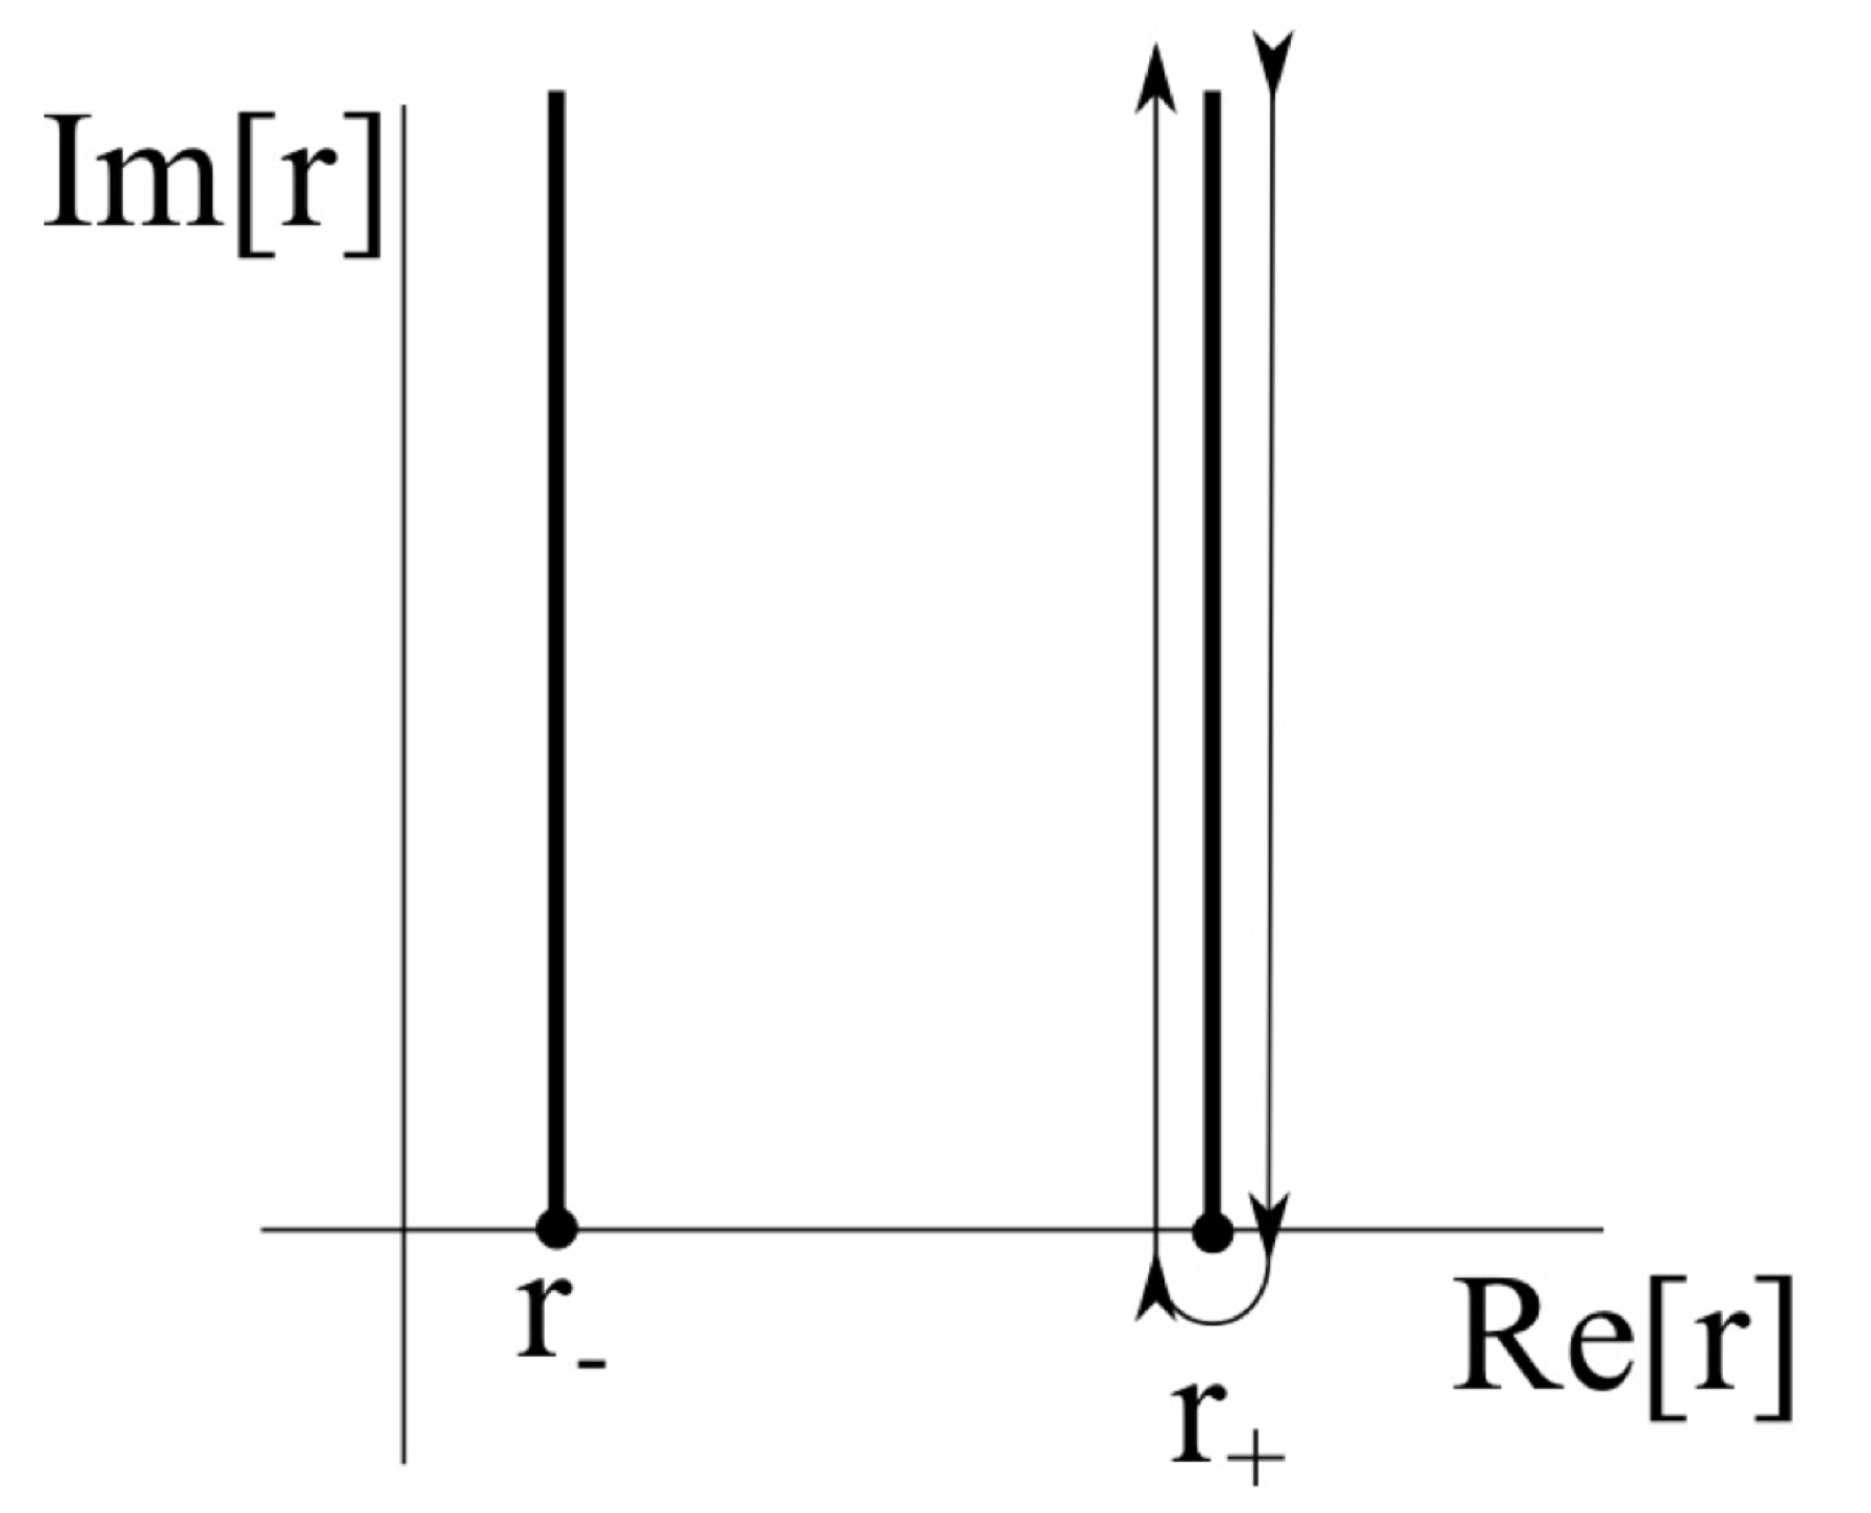
\includegraphics[width=1.0\columnwidth]{chapter_KN_QNM/etc/contour1}
\caption{The contour $\mathscr{C}$ used in the definition of the product \eqref{prod}. The Kerr wave functions $\psi_s^{(0)}$ are analytic everywhere except for two branch cuts emerging from the horizons $r_\pm$ and shooting off to positive infinity. }
\label{fig:contour}
\end{figure}

\subsection{Numerical calculations} 
The spin-$s$ QNMs of a Kerr black hole are indexed by spheroidal harmonic indices $\ell$ and $m$, and an overtone number $n$. For a given $s$, $a$, $\ell$ and $m$, the least damped QNM is assigned $n=0$ (at least when there is no mode branching, see \cite{Yang2012b}).
We label the frequency corrections $\omega^{(1)}$ with the same indices as the corresponding background Kerr frequency $\omega^{(0)}$, grouping them as $\ell m n$. We only discuss the modes with $m \geq 0$ because of the symmetry $\omega(a,m) = \omega(-a,-m)$.

We explore the weakly charged KN QNM frequency spectrum by numerically evaluating Eq.~\eqref{freqform} for $\omega^{(1)}$. We use Leaver's continued fraction method to calculate the Kerr QNM frequencies $\omega^{(0)}$ and a truncated version of Leaver's expansion~\cite{Leaver1985} to represent the Teukolsky wave function $\psi_s^{(0)}$.
We estimate the error in our method by performing the numerical integration twice for each mode, the second time keeping more terms in the wave function expansions and continued fractions, and also more points in the angular integral. We find that the fractional difference $|\omega^{(1)}_\text{run 2}-\omega^{(1)}_\text{run 1}|/|\omega^{(1)}_\text{run 2}|$ is roughly $10^{-6}$. We test the EVP method by applying it to the DF equation (i.e. we replace $\mathcal{H}_s$ with $\mathcal{F}_s$).  
The ``true'' DF QNM frequencies $\omega$ can be obtained via Leaver's method \cite{BertiKokkotas2005}, allowing $\omega^{(1)}$ to be computed independently of the EVP method via a numerical evaluation of $(\omega-\omega^{(0)})/q$ as $q \to 0$. 
In this way we find that the fractional error in $\omega^{(1)}$ is approximately $10^{-5}$.
The possible sources for these small errors are the truncation of the QNM wave functions, numerical imprecision in implementing the contour integral, and error in the root finding step of Leaver's method.

\begin{figure}[t]
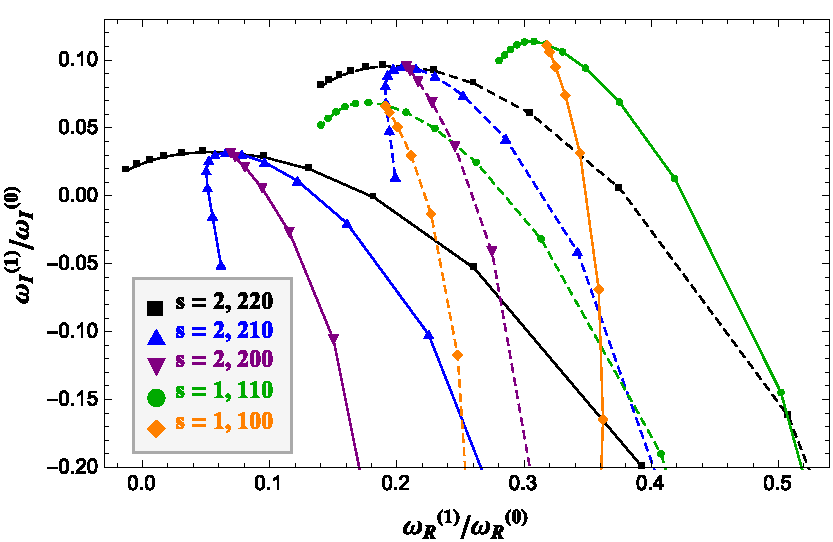
\includegraphics[width=1.0\columnwidth]{chapter_KN_QNM/etc/PRLFig1TopSept17}
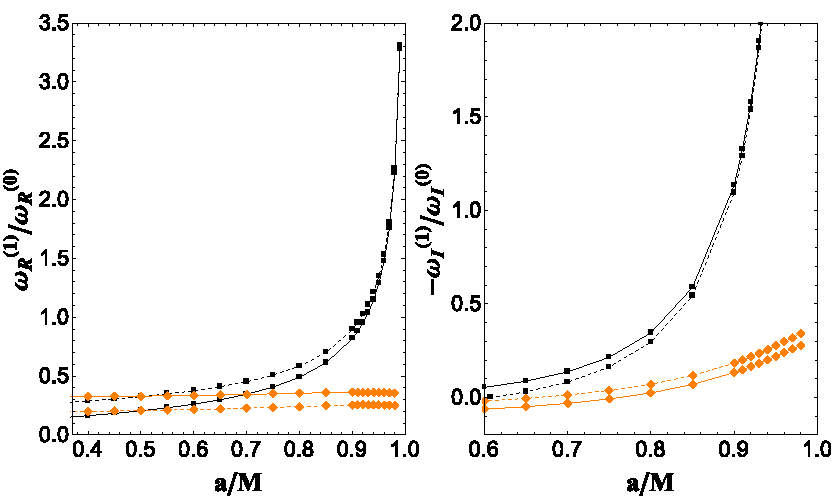
\includegraphics[width=1.0\columnwidth]{chapter_KN_QNM/etc/PRLFig1BotSept17}
\caption{The frequency corrections $\omega^{(1)}$ as predicted by the KN equations \eqref{fun} (solid lines) and by the DF equation (dashed lines). Top panel: scaled frequency corrections $\omega^{(1)}_R/\omega^{(0)}_R+i\omega^{(1)}_I/\omega^{(0)}_I$ as a function of $a/M$. Only the modes with $m \geq 0$ are plotted, and each subsequent data point increases by $0.15$ in $a/M$ (left to right), beginning with $a/M = -0.95$ for the $m=1,2$ modes and with $a/M=0$ for the $m=0$ modes. Bottom panels: The $s=2, 220$ and $s=1, 100$ QNM frequencies plotted versus $a/M$ in the rapidly-rotating regime.}
\label{fig:Corrections}
\end{figure}

In the top panel of Fig.~\ref{fig:Corrections}, we parametrically plot $\omega^{(1)}_R/\omega^{(0)}_R+i\omega^{(1)}_I/\omega^{(0)}_I$ in the complex plane as a function of $a/M$, for eight low-$\ell$ modes. We compute both $\omega^{(1)}$ as predicted by the linearized KN equations (solid lines), using Eq.~\eqref{freqform}, and as predicted by the corresponding EVP analysis for DF equation (dashed lines).
We observe that in general there is a significant difference between the DF frequency corrections and the KN frequency corrections. The bottom panel of Fig.~\ref{fig:Corrections} focuses on the frequency corrections for rapidly-rotating black holes.
We plot $\omega^{(1)}_R/\omega^{(0)}_R$ and $\omega^{(1)}_I/\omega^{(0)}_I$ versus $a/M$ for large values of $a/M$. Notice that as $a \to M$, the DF equation predicts an increasingly accurate frequency correction $\omega^{(1)}$ for the $s=2$, $220$ mode, but not for the $s=1$, $100$ mode. 
We only plot two modes for clarity, but we also found that the DF equation becomes increasingly accurate as  $a \to M$ for the $s=1$, $110$ mode, but not for the $s=2$, $210$ or the the $s=2$, $200$ modes.

Using  Eq.~\eqref{freqform}, we can understand this phenomenon analytically. In the nearly extremal Kerr spacetime, there are two branches of QNMs \cite{Yang2012b, Yang:2013uba}; the Zero Damping Modes (ZDMs), which have zero decay in the extremal limit $a \to M$~\cite{Detweiler1980,Hod2008a}, and the Damped Modes (DMs), which retain a finite decay in this limit. The $s=2$, $220$ mode and the $s = 1$, $110$ mode are both ZDMs, while the $s=2$, $210$; $s=2$, $200$; and the $s=1$, $110$ modes are all DMs. By expanding the Teukolsky equation in powers of $\epsilon \equiv 1-a/M$, one can show that near the horizon ($r-r_+<\sqrt{\epsilon}$), the Kerr ZDMs depend on $\epsilon$ only through
the conformal variable $x \equiv (r-1)/\sqrt{\epsilon}$~\cite{TeukolskyPress1974,Yang:2013uba}, 
while DMs do not vary much with $\epsilon$ in the $\epsilon \rightarrow 0$ limit. Further, when analytically continued onto the contour $\mathscr{C}$, the ZDM wave function is concentrated in the near horizon region, allowing the integral $\eqref{prod}$ to be performed only over the near horizon region $x \ll 1$. 
Thus, we can figure out how the different terms in the formula for $\omega^{(1)}$ scale with $\epsilon$, if we write $\mathcal{F}_s$ and $\mathcal{H}_s$ in terms of the variable $x$ and then pick off the leading order $\epsilon$-dependence. The scalings are
\begin{align}
\frac{\partial \mathcal{F}_s}{\partial q}=\mathcal{O}(\epsilon^{-1}),\;\; \frac{\partial (\mathcal{H}_s-\mathcal{F}_s)}{\partial q} = \mathcal{O}(1) , \; \; 
 \frac{\partial \mathcal{H}_s}{\partial \omega} = \mathcal{O}(\epsilon^{-1/2}) \,.\label{scalings}
\end{align}
The DF equation predicts increasingly accurate frequency corrections as $\epsilon \to 0$ for modes which correspond to Kerr ZDMs because the term that it neglects in Eq.~\eqref{freqform} is $\mathcal{O}(\sqrt\epsilon)$, which is of subleading order.

If we assume that our first order analysis in $q$ is accurate all the way up to $q_\text{max}$, none of the eight modes that we consider become unstable before they reach extremality. To estimate how large $Q$ can get before higher order contributions (in $q$) become important, we use the EVP method to calculate the leading order correction $\omega^{(1)}$ to the QNM frequencies of the DF equation.
We then calculate the residual error in the first order analysis $\delta \omega = \omega -\omega^{(0)} -q\omega^{(1)}$, where $\omega$ is the DF frequency calculated using Leaver's method, and compare it to $q\omega^{(1)}$. Figure \ref{fig:LimFirst} plots the comparison versus $Q/Q_\text{max}$ for the $s=2$, $220$ mode and selected values of $a$. We see that the importance of the higher order contributions varies greatly with $a$. Figure \ref{fig:LimFirst} also reveals that for most modes the first order analysis begins to fail long before $Q =Q_\text{max}$, indicating that going beyond linear analysis is likely necessary for NEKN QNMs.
However, there are some modes, such as the $a=-0.8\, M$, $s=2$, 220 mode, where the first order analysis is reasonably accurate, even when $Q = Q_\text{max}$.
While we have focused on the fundamental $\ell = 1$ (dipolar EM) and $\ell =2$ (quadrupolar GW) modes, we expect our stability results to hold for larger $\ell$ values, since for Kerr QNMs $\omega_I$ is weakly dependent on $\ell$ for large $\ell$ \cite{Yang2012a}.

\begin{figure}[t]
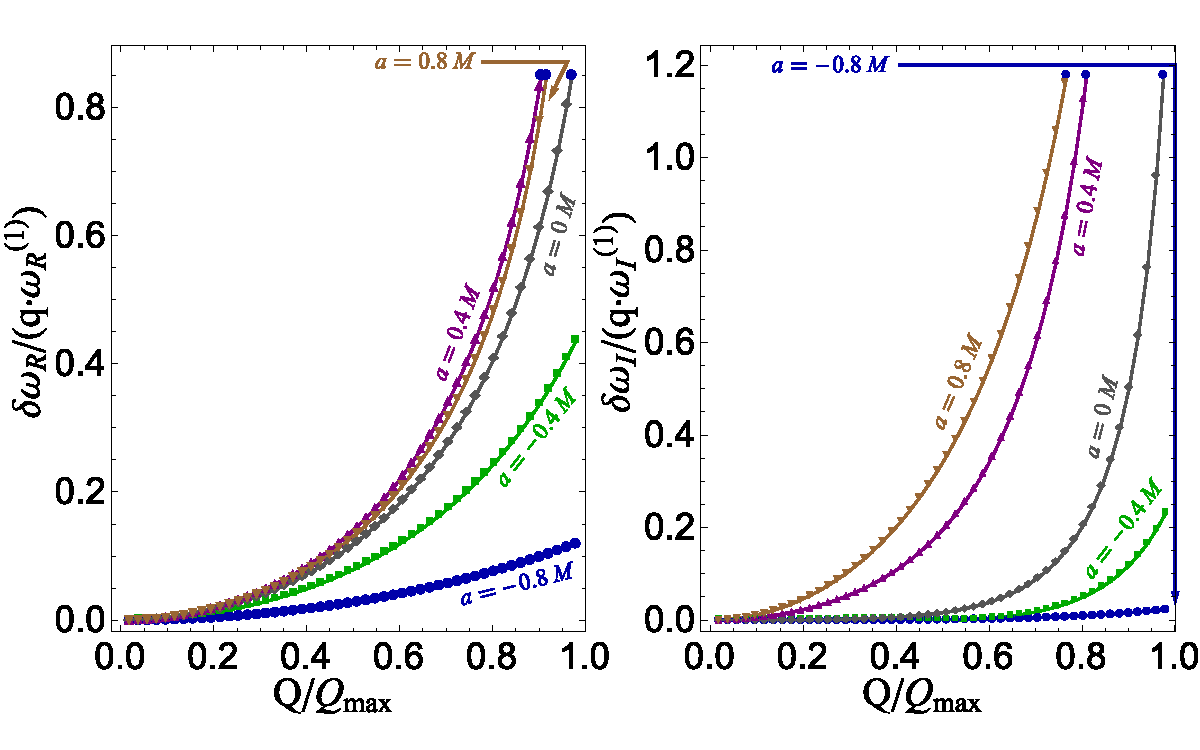
\includegraphics[width=1.0\columnwidth]{chapter_KN_QNM/etc/PRLFig2Sept17}
\caption{Estimate of the size of higher order corrections in $q$, based on the EVP method applied to the DF equation. The residual error in the first order analysis is $\delta \omega = \omega -\omega^{(0)} -q\omega^{(1)}$, where $\omega$ is the true DF frequency calculated using Leaver's method. }
\label{fig:LimFirst}
\end{figure}

{\it Nearly Extremal Kerr-Newman.---} We now examine the modal stability of the weakly charged NEKN spacetime ($q < q_\text{max} =  2\epsilon -\epsilon^2 \ll 1$), where we have 
\begin{align}
\omega(\epsilon, q)=\omega^{(0)}(\epsilon)+\omega^{(1)}(\epsilon) q+ \omega^{(2)}(\epsilon) q^2+ \dots \,. \label{rapqexp}
\end{align}
Numerical searches and nearly extremal expansions \cite{ZimmermanDF} reveal that the extremal DF equation predicts marginally stable modes (ZDMs) for any value of $Q$, while previous work has not found ZDMs in the RN spacetime~\cite{Onozawa:1995vu, Andersson1996}. 
This tension can be resolved by working with the true KN perturbation equations. Suppose that $\omega^{(0)}$ is a Kerr ZDM. A nearly extremal analysis~\cite{Yang2012b} shows that $\omega_I^{(0)}=\mathcal{O}(\sqrt \epsilon)$. 
Substituting the scalings \eqref{scalings} into Eq.~\eqref{freqform}, reveals that $\omega^{(1)}=\mathcal{O}(\epsilon^{-1/2})$. The total charge correction $q \omega^{(1)}$ is in fact the same order as $\omega_I^{(0)}$ since $q_\text{max}\omega^{(1)}(\epsilon) =\mathcal{O}(\sqrt \epsilon)$, and may lead to a growing mode. 
Given our intuition from Fig.~\ref{fig:LimFirst}, confirming the existence of such a mode would require knowledge of the higher order charge corrections $q^j \omega^{(j)}$, which may also scale as $\mathcal{O}(\sqrt \epsilon)$. The stability of NEKN black holes and the possible existence of ZDMs remains an important open question which will be the subject of future investigation.
 
\section{Future Work}
Our analysis provides the first calculation of the KN QNM frequencies for black holes with rapid rotation, and opens many avenues for the application of these results. A clear next step is to extend the analysis by computing the $\mathcal{O}(q)$ corrections to the wave functions, deepening our understanding of the coupling between the gravitational and electromagnetic field, and the $\mathcal{O}(q^2)$ frequency corrections, providing a better estimate of the error in the $\mathcal{O}(q)$ frequencies.

Finally, our analysis of NEKN black holes raises the question of whether ZDMs exist for nearly extremal black holes with arbitrary charge, which can be addressed with a more complete NEKN analysis. 
This would be complemented by a WKB analysis of the coupled equations~\eqref{fun}, which would give further insights into the KN QNMs, the existence of ZDMs and DMs, and the possible geometric correspondence of the QNMs with geodesics~\cite{Mashhoon1985,Yang2012a} and the $s=0$ wave equation in KN.

\section{Acknowledgments}
ZM would like to thank his undergraduate advisor Rob Owen for extensive discussions, both pedagogical and technical, and for looking over drafts of his thesis, which covers some of the same material. The authors also thank Luis Lehner and Yiqiu Ma for conversations about perturbations of KN black holes. AZ, HY, and YC were supported by NSF Grant PHY-1068881, CAREER Grant 0956189, and the David and Barbara Groce Startup Fund at Caltech. ZM was supported by the LIGO SURF program at Caltech. This research was supported in part by the Perimeter Institute for Theoretical Physics. Research at the Perimeter Institute is supported by the Government of Canada through Industry Canada and by the Province of Ontario through the Ministry of Research and Innovation.

\section{Appendix: The Perturbed Kerr-Newman Spacetime in the Newman-Penrose Formalism}

The Newman-Penrose (NP) formalism \cite{ChandraBook, StewartBook, NewmanPenrose1962} is a null-tetrad formulation of General Relativity that offers a simple way of describing spacetimes with one or more sheer-free congruences of null geodesics. Like the Kerr spacetime, the Kerr-Newman (KN) spacetime possesses two such congruences and as a consequence when an appropriate tetrad is chosen the spin coefficients $\kappa$, $\sigma$, $\lambda$, and $\nu$, the Weyl scalars $\Psi_0$, $\Psi_1$, $\Psi_3$, and $\Psi_4$, as well as the Maxwell scalars $\phi_0$ and $\phi_2$ vanish. Hence, in the perturbed KN spacetime these quantities are all of perturbative order and the linearized NP field equations are greatly simplified.  

Despite the similarity in the NP descriptions of the Kerr and KN spacetimes, the perturbed KN spacetime is far more complicated than the perturbed Kerr spacetime. 
While gravitational perturbations and electromagnetic perturbations can be independently excited in the Kerr spacetime, they are necessarily intricately intertwined in the KN spacetime. 
Thus, the perturbed KN spacetime contains two families of perturbations; one family becomes the gravitational perturbations in the $Q \to 0$ limit, while the other family becomes the electromagnetic perturbations. 

In the perturbed KN spacetime (using the appropriate tetrad), the Weyl scalars $\Psi_0$ and $\Psi_4$ are gauge invariant (under infinitesimal tetrad transformations) and they describe gravitational waves near the horizon and near null infinity, respectively.  The rest of the Weyl scalars and Maxwell scalars are not gauge invariant, as is also true in the perturbed Kerr spacetime. There are two convenient gauges to consider. In the perturbed Kerr spacetime, the standard choice is to set $\Psi_1$ and $\Psi_3$ equal to zero by the appropriate infinitesimal tetrad transformation. This means that $\phi_0$ and $\phi_2$  are nonzero and they  describe electromagnetic radiation near the horizon and near infinity, respectively. Alternatively, one can use the ``phantom gauge'' \cite{ChandraBook} and set $\phi_0$ and $\phi_2$ equal to zero. The Weyl scalars $\Psi_1$ and $\Psi_3$ then contain the information describing the electromagnetic field. One way of understanding this is that knowledge of $\Psi_1$ and $\Psi_3$ is necessary to recover  $\phi_0$ and $\phi_2$ in the standard gauge choice. In either gauge, the NP equations contain coupling between gravitational perturbations ($\Psi_0$ and $\Psi_4$) and electromagnetic perturbations ($\phi_0$ and $\phi_2$ or $\Psi_1$ and $\Psi_3$). For our work, we adopt the phantom gauge because the linearized NP field equations appear to be simplest in the phantom gauge. 

We now use the least coupled, linearized NP equations to derive a pair of coupled equations governing $\Psi_0$ and $\Psi_1$ (or $\Psi_3$ and $\Psi_4$). The are many ways of obtaining such equations, but the equations that we arrive at reduce to the Teukolsky equation in the $Q \to 0$ limit and clarify the relationship of the DF equation to the ``true'' KN linearized equations.

We follow Chandrasekhar, using the Kinnersley tetrad and Boyer-Linquist coordinates, and we expand all NP quantities in frequency and azimuthal harmonics  $e^{-i\omega t+im\phi}$. We also adopt Chandrasekhar's notation, defining the following operators which arise when the directional derivative operators $\mathbf{D}$, $\mathbf{\Delta}$, $\boldsymbol{\delta}$, and $\boldsymbol{\delta}^*$ act on functions that are expanded in frequency and azimuthal harmonics:
\begin{align}
&\DD_j \equiv \partial_r+\frac{iK}{\Delta}+2j\frac{(r-M)}{\Delta},& \nonumber
\\ &\DD_j^\dagger \equiv \partial_r-\frac{iK}{\Delta}+2j\frac{(r-M)}{\Delta},& \nonumber
\\ &\LL_j \equiv \partial_\theta+\hat{Q}+j\cot\theta,& \nonumber
\\ &\LL_j^\dagger \equiv \partial_\theta-\hat{Q}+j\cot\theta,& \nonumber
\\ &K=-(r^2+a^2)\omega+am,& \nonumber \\
&\Delta = r^2 -2Mr+a^2+q,& \nonumber \\
&\hat{Q}=-a\omega\sin\theta+\frac{m}{\sin\theta}.& \nonumber
\end{align}
We define spin weighted fields that capture the gravitational and electromagnetic degrees of freedom.
\begin{align}
&\psi_{-2} =\p^{*4}\Psi_4,& &\psi_{-1}=\frac{\p^{*3}\Psi_3}{\sqrt{2}},& \nonumber 
\\ &\psi_1=\sqrt{2} \p^*\Psi_1,& &\psi_2=\Psi_0,& \nonumber
\end{align}
where $\bar{\rho}=r+ia\cos\theta$, $\bar{\rho}=r-ia\cos\theta$, and the prefactors  are necessary to separate the Teukolsky equation in Kerr.
Further, we define scaled versions of the spin coefficients
\begin{align}
k=\frac{\kappa}{\sqrt{2}\p^{*2}}, & & s=\frac{\p\tilde\sigma}{\p^{*2}}, & & \ell =\frac{\p^*\lambda}{2}, & &n=\frac{\rho^2\nu}{\sqrt{2}},
\end{align}
where $\rho^2=\bar \rho \bar \rho^*$.

We begin by linearizing the NP equations Chandrasekhar Ch. 1, (321a) (a Bianchi Identity), (321e) (a Bianchi Identity),  (310b) (a Ricci Identity); Chandrasekhar Ch 11, (136) (a manipulated version of several Maxwell equations); and their GHP transforms \cite{GHP}. The first set of four equations, from which we derive a pair of coupled equations governing $\psi_1$ and $\psi_2$, are expressed in Boyer-Lindquist coordinates as:
\begin{align}
&\left[\LL_2-\frac{3ia\sin\theta}{\p^*} \right]\psi_2 -\left[\DD_0+\frac{3}{\p^*}\right]\psi_1& \nonumber \\
& =-2k\left[3\left(M-\frac{Q^2}{\p}\right)+\frac{Q^2\p^*}{\p^2}\right],& \label{j1}
\\ &\Delta\left[\DD_2^\dagger-\frac{3}{\p^*}\right]\psi_2+\left[\LL_{-1}^\dagger+\frac{3ia\sin\theta}{\p^*}\right]\psi_1& \nonumber \\
&=2s\left[3(M-\frac{Q^2}{\p})-\frac{Q^2\p^*}{\p^2}\right],& \label{j2}
\end{align}
\begin{align}
&\left[\DD_0+\frac{3}{\p^*}\right]s-\left[\LL_{-1}^\dagger+\frac{3ia\sin\theta}{\p^*}\right]k=\frac{\p}{\p^{*2}}\psi_2 \,, \label{j3}
\\ &\Delta\left[\DD_2^\dagger-\frac{3}{\p^*}\right]k+\left[\LL_2-\frac{3ia\sin\theta}{\p^*}\right]s=2\frac{\p}{\p^{*2}}\psi_1 \,. \label{j4}
\end{align}
The GHP transformed versions of these particular equations, from which we derive a pair of coupled equations governing  $\psi_{-1}$ and $\psi_{-2}$, are obtained by replacing 
\begin{align}
&\psi_1 \to -\psi_{-1}, &k \to -n, \nonumber 
\\& \LL_{-1}^\dagger \to \LL_{-1}, & \left[ \DD_0 +\frac{3}{\bar \rho^*}\right] \to \Delta \left[ \DD_{-1}^\dagger +\frac{3}{\bar \rho^*}\right], \nonumber
\\ & \psi_2 \to \psi_{-2}, & s \to \ell, \nonumber \\
&\LL_2 \to \LL_2^\dagger, & \Delta\left[\DD_2^\dagger -\frac{3}{\bar \rho^*}\right] \to \left[\DD_0 -\frac{3}{\bar \rho^*}\right]. \nonumber
\end{align}
As we are trying to get our equations in a form similar to that of the Teukolsky equation, we apply the same manipulations to the KN perturbation equations that decouple the Teukolsky equation. We obtain equations for $\psi_{-2}$, $\psi_{-1}$, $\psi_1$, and $\psi_2$ coupled to only the spin coefficients (in the $Q=0$ case, there is no coupling to the spin coefficients and these equations are the Teukolsky equations) by making use of the commutation relation
\begin{align}
\left[\DD+\frac{c}{\p^*}\right]\left[\LL+\frac{iac\sin\theta}{\p^*}\right]=\left[\LL+\frac{iac\sin\theta}{\p^*}\right]\left[\DD+\frac{c}{\p^*}\right], \label{mcrel}
\end{align}
where $\DD$ represents any of the $\DD_j$ operators or $\DD^\dagger_j$ operators of any $j$, $\LL$ represents any of the $\LL_{j'}$ operators or $\LL^\dagger_{j'}$ operators, of any $j'$ ($j'$ does not have to equal $j$), and $c$ is any constant. The simplified equations are
\begin{align}
&\left(\Delta\DD_1\DD_2^\dagger+\LL_{-1}^\dagger\LL_2+6i\omega\p\right)\psi_2 \nonumber \\
&=-2Q^2\left[\LL_{-1}^\dagger\left(\frac{\p^*k}{\p^2}\right)+\DD_0\left(\frac{\p^*s}{\p^2}\right)\right], \label{p1}
\\ & \left(\Delta\DD_2^\dagger\DD_0+\LL_2\LL_{-1}^\dagger+6i\omega\p\right)\psi_1 \nonumber 
\\ &=2Q^2\left[\Delta\DD_2^\dagger\left(\frac{\p^*k}{\p^2}\right)-\LL_2\left(\frac{\p^*s}{\p^2}\right)\right], \label{p2}
\\& \left(\Delta\DD_1\DD_{-1}^\dagger+\LL_2^\dagger\LL_{-1}-6i\omega\p\right)\psi_{-1} \nonumber \\
&= 2Q^2\left[\DD_0\left(\frac{\p^* n}{\p^2}\right)+\LL_2^\dagger\left(\frac{\p^*\ell}{\p^2}\right)\right], \label{p3}
\\& \left(\Delta\DD_{-1}^\dagger\DD_0+\LL_{-1}\LL_2^\dagger-6i\omega\p\right)\psi_{-2} \nonumber \\
&= -2Q^2\left[-\LL_{-1}\left(\frac{\p^* n}{\p^2}\right)+\Delta\DD_{-1}^\dagger\left(\frac{\p^* \ell}{\p^2}\right)\right]. \label{p4}
\end{align}
We arrive at our desired equations by solving Eqs.~\eqref{j1}, \eqref{j2}, and their GHP transforms for $k$, $s$, $n$, and $\ell$ and inserting the resulting expressions into Eqs.~\eqref{p1}, \eqref{p2}, \eqref{p3}, and \eqref{p4}. The final equations are
\begin{equation}
\begin{bmatrix}
\mathcal{F}_{\pm2}+ q\mathcal{G}_{\pm2}  & q\delta \mathcal{H}_{\pm2} \\ \\
q \delta \mathcal{H}_{\pm1} &  \mathcal{F}_{\pm1} +q\mathcal{G}_{\pm1}
\end{bmatrix}
\begin{bmatrix}
\psi_{\pm2} \\
\psi_{\pm1}
\end{bmatrix}
=0.
\label{fun2}
\end{equation}
The $\mathcal{F}_s$, $\mathcal{G}_s$, and $\delta \mathcal{H}_s$ operators are defined in Table \ref{table}, where we have defined $\alpha_\pm \equiv \left[3(\p^2M-\p Q^2)\pm Q^2\p^*\right]^{-1}$ in order to simplify the expressions. The $\mathcal{F}_s$ operator is the spin $s$ DF operator, which becomes the Teukolsky operator in the $Q \to 0$ limit. The only $q$ dependence in $\mathcal{F}_s$ comes from $\Delta$, and the DF equation can be understood as the Teukolsky equation with modification $\Delta_\text{kerr} =r^2-2Mr+a^2 \to \Delta$. The $\mathcal{O}(1)$ operator $\delta\mathcal{H}_s$ introduces an $\mathcal{O}(q)$ coupling term into the perturbation equations. Finally, the operator $q\mathcal{G}_s \psi_s$ is the $\mathcal{O}(q)$ difference between the $\mathcal{H}_s$ term and the $\mathcal{F}_s$ term in Eq.~\eqref{fun2} alluded to in the body of the paper. The $\mathcal{F}_s$ and $\mathcal{G}_s$ operators are important to the $\mathcal{O}(q)$ analysis of the EVP method, while the  $\delta\mathcal{H}_s$ operator comes in at higher order and can be neglected.

%\onecolumngrid
%   \begin{tabular}{ | c | c | c |  c|}

\begin{table}[h]
\begin{center}
    \begin{tabular}{ | c | p{1.5in} | p{1.5in} |  p{1.5in}|}
    \hline
    $s$ & $\mathcal{F}_s f$ & $\mathcal{G}_s f$ & $\delta\mathcal{H}_s f$ \\ \hline
  2 & $ \Delta \DD_1\DD_2^\dagger f +\LL_{-1}^\dagger\LL_2 f+6i\omega\bar\rho f$
 & $\LL_{-1}^\dagger \alpha_+3ia\sin\theta f-\LL_{-1}^\dagger \alpha_+\p^*\LL_2 f$ & $\LL_{-1}^\dagger\alpha_+\p^*\DD_0f+3\LL_{-1}^\dagger\alpha_+f $\\ & &$+\DD_0\alpha_-\Delta\p^*\DD_2^\dagger f-3\DD_0\alpha_- \Delta f$ & $+\DD_0\alpha_-\p^*\LL_{-1}^\dagger f+3\DD_0\alpha_-ia\sin\theta f$  \\ \hline
    1 & $ \Delta \DD_2^\dagger\DD_0 f +\LL_{2}\LL_{-1}^\dagger f+6i\omega\bar\rho f$ & $-\Delta\DD_2^\dagger\alpha_+\p^*\DD_0f-3\Delta\DD_2^\dagger\alpha_+f$ & $-3\Delta\DD_2^\dagger\alpha_+ia\sin\theta f+\Delta\DD_2^\dagger\alpha_+\p^*\LL_2f$ \\ & &$+\LL_2\alpha_-\p^*\LL_{-1}^\dagger f+3\LL_2\alpha_-ia\sin\theta f$ & $+\LL_2\alpha_-\Delta\p^*\DD_2^\dagger f-3\LL_2\alpha_-\Delta f $\\ \hline
    -1 & $\Delta\DD_1\DD_{-1}^\dagger f+\LL_2^\dagger\LL_{-1}f-6i\p\omega f$ & $- \DD_0 \alpha_+ \p^* \Delta \DD_{-1}^\dagger f -3 \DD_0 \alpha_+ \Delta f$ & $-\DD_0 \alpha_+ \p^* \LL_2^\dagger f +3 \DD_0 \alpha_+ ia \sin \theta f$ \\ & &$\LL_2^\dagger \alpha_- \p^* \LL_{-1} f +3 \LL_2^\dagger \alpha_- i a\sin\theta f$ &$-\LL_2^\dagger \alpha_- \p^* \DD_0 f +3 \LL_2^\dagger \alpha _- f$ \\ \hline
    -2 & $\Delta\DD_{-1}^\dagger\DD_0 f+\LL_{-1}\LL_2^\dagger f-6i\p\omega f$& $\Delta \DD_{-1}^\dagger \alpha_-\p^*\DD_0 f -3\Delta \DD_{-1}^\dagger \alpha_- f$ & $-\Delta \DD_{-1}^\dagger \alpha_- \p^* \LL_{-1} f -3 \Delta \DD_{-1}^\dagger \alpha_- i a \sin \theta f$ \\ &  &$- \LL_{-1}\alpha_+ \p^* \LL_2 ^\dagger f +3 \LL_{-1} \alpha_+ i a \sin \theta f$ & $-\LL_{-1} \alpha_+ \p^* \Delta \DD_{-1}^\dagger f -3\LL_{-1} \alpha_+ \Delta f$ \\ \hline
    \end{tabular} 
\end{center} 
\caption{The definitions of the $\mathcal{F}_s$, $\mathcal{G}_s$, and $\delta \mathcal{H}_s$ operators.}
\label{table}
\end{table}



%\twocolumngrid


\printbibliography[heading=subbibliography]
\end{refsection}
%\begin{refsection}

\newcommand{\ba}{\begin{align}}
\newcommand{\ea}{\end{align}}
\newcommand{\bma}{\begin{pmatrix}}
\newcommand{\ema}{\end{pmatrix}}
\newcommand{\R}[1]{\textcolor{red}{#1}}

\chapter{Damped and zero-damped quasinormal modes of charged, nearly-extremal black holes}
\label{chap:Extremal}

\begin{centering}
Aaron Zimmerman and Zachary Mark \\
Phys. Rev. D 93, 044033 (2016) \\
\href{https://https://arxiv.org/abs/1512.02247}{arxiv:1512.02247} \\
\end{centering}

\section{abstract}
Despite recent progress, the complete understanding of the perturbations of charged, rotating black holes as described by the Kerr-Newman metric remains an open and fundamental problem in relativity.
In this study, we explore the existence of families of quasinormal modes of Kerr-Newman black holes whose decay rates limit to zero at extremality, called zero-damped modes in past studies.  
We review the nearly-extremal and WKB approximation methods for spin-weighted scalar fields (governed by the Dudley-Finley equation) and give an accounting of the regimes where scalar zero-damped and damped modes exist.
Using Leaver's continued fraction method, we verify that these approximations give accurate predictions for the frequencies in their regimes of validity.
In the non-rotating limit, we argue that gravito-electromagnetic perturbations of nearly-extremal Reissner-Nordstr\"{o}m black holes have zero-damped modes in addition to the well-known spectrum of damped modes.
We provide an analytic formula for the frequencies of these modes, verify their existence using a numerical search, and demonstrate the accuracy of our formula. 
These results, along with recent numerical studies, point to the existence of a simple universal equation for the frequencies of zero-damped gravito-electromagnetic modes of Kerr-Newman black holes, whose precise form remains an open question.

\section{Introduction}

The Kerr-Newman (KN) black hole~\cite{Newman:1965my,Adamo:2014baa,Chrusciel:2012jk} is the most general four-dimensional black hole solution to the electro-vacuum Einstein field equations, provided that the unphysical magnetic and NUT charges are set to zero. 
While astrophysical black holes cannot maintain significant charge~\cite{Gibbons1974,Blandford:1977ds}, charged black holes remain fundamental objects of study in gravitational and quantum theories. 
KN black holes are the simplest charged, rotating objects allowed by relativity, and so provide a natural arena to study the interplay of electromagnetism and gravity. 
However, perturbations of these black holes have until recently been poorly understood, even many years after their discovery.

As in other black hole solutions, perturbed KN black holes possess a spectrum of decaying, resonant oscillations. 
These quasinormal modes (QNMs)~\cite{Kokkotas1999,Berti2009} are excited by transient sources, and they decay as energy flows into the black hole horizon and outward to asymptotic infinity. 
In simpler black hole solutions, such as the rotating Kerr black hole~\cite{Kerr:1963ud,Teukolsky:2014vca}, the quasinormal modes can be understood as the eigensolutions to systems of ordinary differential equations, with the QNM frequencies given by the eigenvalues. 
The study of QNMs is an essential topic in understanding the structure of black hole spacetimes. 
QNMs play a role in gravitational wave astrophysics (e.g.~\cite{Dreyer2004,Berti:2005ys,Barausse:2014tra}) where they make up the ``ringdown'' following the birth of a black hole or the merger of two black holes; have connections to quantum field theories through the AdS/CFT correspondence~\cite{Son:2007vk}; and are potentially linked to quantum mechanical excitations of black holes (see the extensive references in~\cite{Berti2009}).

While much is known about the spectrum of Kerr black holes and the non-rotating, charged Reissner-Nordstr{\"o}m (RN) black holes, the investigation of the QNMs of KN black holes has proven difficult outside of the scalar case discussed below.
Gravitational and electromagnetic perturbations of the Kerr black hole can be tackled by studying spin-weighted scalar fields propagating on the black hole background.
These scalars obey a master equation~\cite{Teukolsky1973}, which separates into coupled ordinary differential equations.
When these same methods are applied to applied to the KN black hole, the result is a system of equations describing coupled gravitational and electromagnetic perturbations~\cite{ChandraBook,Dias:2015wqa}. While these equations can still be expanded in frequency and azimuthal harmonics due to the symmetries of the spacetime, they have not been separated in the remaining coordinates. 
In contrast, for the spherically-symmetric RN black hole, separation is possible and equations for coupled ``gravito-electromagnetic'' (GEM) perturbations can be derived~\cite{Moncrief:1974ng, Moncrief:1974gw, Zerilli:1974ai}. Using these equations, the QNMs of RN have been extensively studied~\cite{Berti2009}.

The difficulties in analyzing the perturbations of KN black holes led to the exploration of simpler wave equations on the KN background, in the hope that they might provide a reasonable approximation to the full problem. 
In particular, Kokkotas and Berti studied the QNMs of the Dudley-Finley (DF) equation on the KN backgrounds~\cite{Kokkotas:1993ef,Berti:2005eb}. 
The DF equation~\cite{Dudley:1977zz,Dudley:1978vd} describes the propagation of spin-weighted test fields in various spacetimes. 
Of particular interest is Type D spacetimes such as KN, where the DF equation separates. 
In this case, the DF equation can be reduced to a coupled eigenvalue problem for the QNMs, just as for the perturbations of the Kerr black hole.
In the spin-zero case, $s=0$, the DF equation reduces to the wave equation for a massless, uncharged scalar field, $\nabla^\mu \nabla_\mu \psi = 0$. Thus the analysis of the $s = 0$ DF equation yields the true scalar QNMs of the KN black hole. 
For $s\neq 0$, the QNMs can only be an approximation (and possibly a poor one) to the QNMs of the gravitational and electromagnetic perturbations of KN.
The DF equations assume that each test field is treated independently\footnote{For example, one can show using the methods in~\cite{Teukolsky1973} that the DF equation is obeyed by a second fictitious set of Maxwell fields propagating on the KN background, which have no leading order background contributions.}, which does not correctly capture the coupling between the electromagnetic and gravitational perturbations of KN.
Although there has been some confusion in the literature on this point, there is no reason a priori to expect that the DF equation provides anything more than a qualitative description of the QNMs of 
KN\footnote{For example, the study~\cite{Hod:2008se} assumes that the DF equation provides a description of the the QNMs of slowly-rotating KN black holes; the results given there only approximate the scalar QNM frequencies of NEKN.}. 

Recently, a great deal of progress has been made in understanding the true GEM modes of KN black holes. 
New approximation techniques have allowed for the investigation of KN black holes which deviate from Kerr and RN black holes by small amounts. 
Slowly rotating, charged black holes were treated using using a matrix-valued continued fraction method~\cite{Pani:2013ija,Pani:2013wsa}. 
Following this, Mark et al.~\cite{Mark:2014aja} tackled the case of a weakly-charged KN black hole, using an eigenvalue perturbation method adapted for quasinormal modes~\cite{Yang:2014tla, Zimmerman:2014aha}.
Most excitingly, challenging numerical studies have allowed the exploration of the QNMs for the full range of angular momentum and charge parameters of KN black holes for the first time~\cite{Zilhao:2014wqa, Dias:2015wqa}. 
The work of Dias, Godazgar, and Santos~\cite{Dias:2015wqa} is especially noteworthy, presenting a complete scan of the $(a,\,Q)$ parameter space of KN black holes, for the lowest overtone and $l\leq 3$.
While this comprehensive information is now in principle available, an analytic understanding of these QNMs remains an important goal.

One region of parameter space which is of special interest and which may be amenable to analytic techniques is the nearly-extremal KN (NEKN) black holes. Kerr-Newman black holes have an extremal combination of charge and angular momentum, which causes their inner and outer horizons to coalesce, and where the surface gravity of the black hole vanishes.
Beyond these extremal combinations of charge and spin the singularity within the black hole is naked to asymptotic infinity, destroying any notion of causality. 
As black holes enter the nearly-extremal regime a new approximation scheme  becomes available, in terms of the small distance from extremality. 
For the Kerr spacetime, the Teukolsky equation simplifies in this limit and approximate formulae for the QNM frequencies are known.
These formulae describe weakly-damped QNMs with the real part of the frequency $\omega$ given by $m \Omega_H$ and the imaginary part proportional to $\sqrt{\epsilon}$~\cite{TeukolskyPress1974,Detweiler1980,Andersson2000,Glampedakis2001,Hod2008a,Yang:2012he,Yang:2012pj,Yang:2013uba}, where $\epsilon  = 1- a/M \ll 1$ is the small expansion 
parameter. 
These modes have been well studied, and were called the zero-damped modes (ZDMs) in~\cite{Yang:2012pj,Yang:2013uba} to distinguish them from a second family of modes, the damped modes (DMs) whose decay remains nonzero in the limit $\epsilon \to 0$. 
The ZDMs can be analyzed in the nearly-extremal limit using a matched asymptotic expansion of the radial equation, and appear to be related to the mathematical horizon instability of extremal black holes~\cite{Aretakis:2012ei,Aretakis:2013dpa,Reiris:2013efa}.
Meanwhile, the DMs must be treated using a different method, either through numerical exploration or the use of a WKB analysis in Kerr~\cite{Yang:2012he}.

Mark et al.~\cite{Mark:2014aja} were able to deal with the case of rapidly-rotating, weakly charged KN black holes. The results of that study hint at the existence of ZDMs in these spacetimes, and surprisingly also show that the DF equation alone provides the correct small-charge perturbation to the ZDM frequencies of Kerr.
In addition, the recent numerical studies of KN QNMs~\cite{Zilhao:2014wqa, Dias:2015wqa} provide strong evidence that for NEKN black holes, the QNM frequencies are described by an equation like that obeyed by the ZDMs of Kerr. 
With these results, one might hope that all the modes of NEKN might be described by a simple equation.


These facts motivate the exploration of both the DF equation and the full GEM equations of KN in the nearly-extremal limit.
The goal of this study is more modest; we give an accounting of those cases where the full problem simplifies.
In Sec.~\ref{sec:DF} we study the DF equation for NEKN black holes. We identify ZDMs which exist for any value of $a$, including the non-rotating case of the nearly-extremal RN (NERN) black hole, by combining analytic approximations and numerical mode searches.
A WKB analysis valid for scalar fields on KN~\cite{HodEikonal2012,Zhao:2015pqa} identifies where modes with nonzero decay exist in the parameter space of extremal KN black holes, implying that in these cases the QNM spectrum bifurcates into two branches as the black hole approaches extremality at fixed angular momentum. 
This bifurcation occurs for certain QNM families of Kerr, as discussed in~\cite{Yang:2012pj,Yang:2013uba}.
We discuss this WKB analysis in Sec.~\ref{sec:WKBanalysis}.
In Sec~\ref{sec:DFNumerics} we use a numerical search to determine the accuracy of the nearly-extremal and WKB approximations, and we also find separated families of DMs and ZDMs.
Note that the frequency formula we derive here for scalar modes of NEKN black holes was presented without derivation in recent note~\cite{Hod:2014uqa}\footnote{That work makes the incorrect claim that the DF equation describes electromagnetic and gravitational perturbations in KN.}.

Motivated by these results for scalar fields, in Sec.~\ref{sec:RN} we show that ZDMs also exist in the case of the GEM modes of NERN, using an analytic approximation and matching ansatz. We confirm the existence of these modes with an explicit numerical search.
These modes are purely decaying with a small decay rate, and they appear to have been overlooked despite a long history of study of the QNMs of RN. 
Such modes give additional support to the conjecture that ZDMs exist for all nearly-extremal black holes, but they also demonstrate the failure of the DF equation to accurately capture the GEM frequencies in this limit.

Finally, we discuss prospects for the open problem of the coupled GEM perturbations of NEKN in Sec.~\ref{sec:Conclusions}.
In this work, we do not attempt to discuss the topic of charged and massive fields on KN backgrounds where superradiant instabilities are found to arise (see e.g.~\cite{Brito:2015oca} for a recent review).

Throughout this paper we use geometric units so that charge and mass have units of length, setting $G = c =1$. We provide a reference for the definitions of some of the important variables used in Table~\ref{tab:VarList}.

\begin{table}
\renewcommand{\arraystretch}{2}
\caption{
\label{tab:VarList}
List of relevant definitions
}
%\begin{ruledtabular}
\begin{tabular}{@{} l c l @{}}
$r_\pm$ & $\displaystyle M \pm \sqrt{M^2 - a^2 -Q^2}$ & Horizon positions \\
$\sigma$ & $\displaystyle \frac{r_+ - r_-}{r_+}$ & Near-extremal parameter \\
$k$ & $\omega - m \Omega_H$ &  Corotating frequency \\
$\hat{\omega}$ & $\omega r_+$ & Dimensionless frequency \\
$ \Omega_H$ & $\displaystyle \frac{a}{r_+^2 +a^2}$ & Horizon frequency \\
$\kappa$ & $\displaystyle  \frac{\sigma r_+}{2(r_+^2 +a^2)}$ & Surface gravity \\
$\mathcal J^2$ & $(m \Omega_H)^2(6M^2 +a^2) - A$ & WKB indicator of DMs \\
$\delta^2$ & $\displaystyle 4 \hat{\omega}^2- (s+1/2)^2 - \lambda$ & DF matching parameter \\
$\varpi$ & $\displaystyle \frac{k}{\kappa}  - i s $ & DF matching parameter \\ 
$\zeta$ & $2m r_+ \Omega_H - i s$ & DF matching parameter \\ 
$x$ & $\displaystyle \frac{r-r_+}{r_+} $ & Radial parameter \\
$\displaystyle{\genfrac{}{}{0pt}{}{\omega_R,} {\omega_I}}$ & $\omega = \omega_R + i \omega_I$ & Frequency components
\end{tabular}
%\end{ruledtabular}
\end{table}


\section{The Dudley-Finely equation for nearly-extremal Kerr-Newman black holes}
\label{sec:DF}

In this section we discuss the QNMs of the Dudley-Finley equation for  nearly-extremal Kerr-Newman black holes.

Due to the similarity between the Teukolsky equation and the DF equation, Leaver's continued fraction method~\cite{Leaver1986}, used to accurately compute the QNMs of Kerr, extends easily to the DF equation in the KN background~\cite{Berti:2005eb}.
This method can in principle provide accurate QNM frequencies for any spin angular momentum, charge, and harmonic.
Since our interest is develop further analytic understanding of the QNM frequencies in the limit of nearly-extremal black holes, we use the nearly-extremal and WKB approximations to explore the ZDM and DM frequencies. 
We then use Leaver's method to confirm these approximations, and to measure their error.


\subsection{Kerr-Newman black holes}

Kerr-Newman black holes are parameterized by their mass $M$, specific angular momentum $a$, and charge $Q$ when magnetic and NUT charges are neglected. One convenient way to represent the metric for the KN spacetime in Boyer-Lindquist coordinates~\cite{BoyerLindquist1967} is obtained by writing the line element of Kerr in terms of the second degree polynomial $\Delta = r^2 - 2 M r+a^2$. The roots of this polynomial are the inner ($r_-$) and outer $(r_+)$ horizons of Kerr, $\Delta = (r-r_+)(r-r_-)$. The Kerr-Newman metric follows from using the appropriate definition of $\Delta$ when charge is included. This form of the line element is~\cite{MTW}
\begin{align}
ds^2  &=  - \frac{\Delta}{\rho^2 } \left(dt - a \sin^2\theta d \phi \right)^2 + \frac{\rho^2}{\Delta} dr^2 + \rho^2 d\theta^2 \notag \\
& \, + \frac{\sin^2 \theta}{\rho^2} \left[a dt - (r^2+a^2)d\phi\right]^2
\,, \\
\Delta  &=  r^2 - 2 M r +a^2 +Q^2 \,, \\
\rho^2  &=  r^2 +a^2 \cos^2 \theta\,.
\end{align}
The corresponding vector potential takes the form 
\begin{align}
A_\mu dx^\mu =\frac{Qr}{\rho^2}\left(dt -a\sin^2\theta d\phi \right)\,.\end{align}
The outer and inner horizons are located at
\begin{align}
r_\pm =  M \pm \sqrt{M^2 - a^2 - Q^2} \,.
\end{align}
In the nearly-extremal limit, where the inner and outer horizons approach each other, we define the small 
parameter\footnote{In~\cite{Yang:2013uba} the small parameter $\epsilon$ is used, while older studies use $\sigma$ as the small parameter. 
Using $\sigma$, the analysis of nearly-extremal Kerr carries over naturally to KN black holes.}
$\sigma \ll1$ as

\begin{align}
\sigma = \frac{r_+ - r_-}{r_+} \approx 2 \sqrt{1 - a^2/M^2 - Q^2/M^2} \,.
\end{align}
It is also useful to recall the expression for the surface gravity $\kappa$ of the KN black hole~\cite{Wald1984}
\begin{align}
\kappa = \frac{r_+ - r_-}{2(r_+^2 +a^2)} = \frac{\sigma r_+}{2(r_+^2 +a^2)} \,.
\end{align}
We see that $r_+ \kappa \ll 1$ in the nearly-extremal limit.

\subsection{The Dudley-Finley equation}

We turn to the analysis of the DF equations in the KN spacetime. 
These equations and their analysis closely parallels the treatment of scalar, electromagnetic, and gravitational perturbations of the Kerr spacetime by using spin-weight $s$ scalars ${}_s \psi$, which obey a separable master equation~\cite{Teukolsky1973}.
Just as in Kerr, we expand the spin-weighted scalars ${}_s \psi$ in frequency and azimuthal harmonics as
\begin{align}
{}_s \psi & = \sum_{lm} \int d\omega \, e^{-i(\omega t - m \phi)} {}_s R_{lm\omega}(r) {}_sS_{lm\omega}(\theta) \,.
\end{align}
With this expansion, the DF wave equations in the KN spacetime separate~\cite{Kokkotas:1993ef} and are nearly identical to the corresponding equations in Kerr.

The angular functions $ {}_sS_{lm\omega}(\theta)$ are spin-weighted spheroidal harmonics and obey the angular Teukolsky equation~\cite{Teukolsky1973,Fackerell1977,Berti2009}, 
\begin{align}
\label{eq:TeukS}
\csc \theta & \frac{d}{d\theta} \left( \sin \theta  \frac{dS}{d\theta}\right) + V_\theta S = 0 \,, \\
V_\theta = & \, a^2 \omega^2 \cos^2 \theta - m^2 \csc^2 \theta - 2 a \omega s \cos \theta \notag  \\ &
- 2 m s \cot \theta \csc \theta -s^2 \cot^2 \theta + s + {}_s A_{lm \omega} \,.
\end{align} 
Here the angular separation constants for each harmonic are denoted ${}_s A_{lm\omega}$.
In the limit of a Schwarzschild black hole ($a \to 0$) they simplify, $A \to l(l+1) - s(s+1)$.

The radial functions ${}_s R_{lm\omega}(r)$ obey a second order differential equation. In the source-free case it is
\begin{align}
\label{eq:TeukR}
\Delta^{-s} & \frac{d}{dr} \Delta^{s+1} \frac{dR}{dr} + V_r R = 0 \,, \\
\label{eq:PotR}
V_r & =  \frac{K^2 + i s K \partial_r \Delta }{\Delta} - 2 i s \partial_r K - {}_s\lambda_{lm\omega} \,, \\
K & = - \omega(r^2+a^2) + am \,, \\
{}_s \lambda_{lm \omega} & = {}_sA_{lm\omega} - 2 a m \omega +a^2 \omega^2\,.
\end{align}
Here and elsewhere we suppress spin-weight and harmonic indices where there is no danger of confusion.

It is useful to define a tortoise coordinate $r_*$ and rewrite the radial equation in terms of a different function ${}_s u_{lm\omega}$. These are defined as follows:
\begin{align}
\frac{dr_*} {dr}& = \frac{r^2 +a ^2} {\Delta} \,, &   u & = \Delta^{s/2} \sqrt{r^2 +a^2} R \,.
\end{align}
With these substitutions, the radial equation~\eqref{eq:TeukR} becomes
\begin{align}
\label{eq:Teuku}
\frac{d^2 u}{dr_*^2}& + V_u u = 0 \,,\\
V_u & = \frac{K^2 + 2 i s K (r- M) + \Delta(4 i s \omega r - \lambda)}{(r^2+a^2)^2} - G^2 -\frac{dG}{dr_*} \,,\\
G & = \frac{\Delta r}{(r^2+a^2)^2} + \frac{s \partial_r \Delta}{2(r^2+a^2)} \,.
\end{align}
Equation~\eqref{eq:Teuku} makes it apparent that the asymptotic solution as $r_* \to - \infty$ (as $r\to r_+$) is the same as in Kerr but with a change in the definition of $k$ and $\Delta$,
\begin{align}
\label{eq:Ingoingu}
u &\sim \exp\left[\pm \frac{s}{2} \frac{\sigma r_+}{r_+^2 +a^2} r_* \right]e^{\pm i k r_*}  = \Delta^{\pm s/2} e^{\pm i k r_*}
 \,, \\
\label{eq:Defk}
k& = \omega - m \frac{a}{r_+^2 +a^2} = \omega - m \Omega_H \,,
\end{align}
where we have identified the horizon frequency $\Omega_H$ in the final expression. 
The asymptotic solution $u \sim \Delta^{-s/2} e^{-ikr_*}$ corresponds to waves traveling into the horizon \cite{Teukolsky1973}.
The second asymptotic solution corresponds to waves which are directed out of the horizon, and we discard this unphysical solution.
Meanwhile, the outer asymptotic solutions remain unchanged from Kerr to KN,
\begin{align}
\label{eq:Outgoingu}
u \sim r^{\pm s} e^{\mp i \omega r_*} && r \to \infty \,.
\end{align}
These solutions correspond to ingoing waves for $u\sim e^{+i\omega r_*}$ and outgoing waves for $u\sim e^{-i\omega r_*}$.
The QNMs of the DF equation can be found by solving the radial equation~\eqref{eq:Teuku} with an outgoing boundary condition; only certain frequencies allow for solutions which also obey the boundary condition at the horizon.

Both the matched asymptotic expansion and the WKB analysis of Kerr carry directly over to the case of the DF equation in KN. 
In the remainder of this section, we discuss these results, which demonstrate the bifurcation of the scalar spectrum of the NEKN black hole into ZDMs and DMs.
These results also set the stage for an understanding of the existence of both ZDMs and DMs for the coupled GEM perturbations of NERN black holes as discussed in Sec.~\ref{sec:RN}. 
For NEKN black holes, either the spin parameter $a$ or the charge $Q$ can be eliminated in favor of $\sigma$. 
We choose to retain an explicit dependence on $a$ in our equations.

\subsection{Matching analysis of the Dudley-Finley equation in nearly-extremal Kerr Newman}
\label{sec:Matching}

To investigate the nearly-extremal modes, we must use the technique of matched asymptotic expansions\footnote{A regular perturbation analysis where the wave function is a power series in $\sigma$ does not work because, in the language of matched asymptotic expansions, there is a boundary layer at the horizon.}.
Our analysis closely follows the analysis of the Kerr case in Yang et al.~\cite{Yang:2013uba} and the references therein. 
For this we define a new coordinate variable $x$ and dimensionless frequency $\hat \omega$ via
\begin{align}
x & = \frac{r - r_+}{r_+} \,,  & \hat \omega &= \omega r_+ \,.
\end{align}
The method splits the region exterior to the black hole into an outer, far-field region $x \gg \sigma$, and an inner, near-horizon region $x \ll 1$. 
The method only works for ZDMs; that is, we assume from the beginning that the frequency has the form $\omega = m \Omega_H + O(\sigma)$. 
First we look at radial equation in the outer region.

\subsubsection{The outer solution}

We rewrite the Teukolsky equation for $R$, Eq.~\eqref{eq:TeukR}, in terms of $x,\, \hat \omega$ and substitute $k$ from Eq.~ \eqref{eq:Defk}.
Using the approximation $\sigma\ll x$, we arrive at the same outer solution as in Kerr,
\begin{align}
\label{eq:TeukFar}
x^2 R'' + 2 (s+1) x R' + \left[\hat \omega^2 (x+2)^2 + 2 i s \hat \omega x - \lambda \right] R = 0 \,.
\end{align}
We define $\delta$ through
\begin{align}
{}_s\delta_{lm\omega}^2 = 4 \hat \omega^2 - (s+1/2)^2 - {}_s\lambda_{lm\omega} \,,
\end{align}
and we find the solution to Eq.~\eqref{eq:TeukFar} in terms of confluent hypergeometric functions ${}_1F_1$~\cite{nist},
\begin{align}
\label{eq:OuterSln}
R =  A &e^{-i \hat \omega x} x^{ -1/2 - s + i \delta} \notag \\
& \times {}_1F_1(1/2-s + i \delta + 2i \hat \omega, 1 + 2 i \delta, 2 i \hat \omega x) \notag \\
& + B (\delta \to - \delta) \,,
\end{align}
where $(\delta \to - \delta)$ indicates that the same functions are repeated with the sign of $\delta$ reversed.
In NEKN $\delta$ no longer takes the explicit form it has in Kerr, $\delta_{\rm K}^2 = 7m^2 / 4 -(s+1/2)^2 - A$, because while the frequency still becomes nearly proportional to the horizon frequency, $\omega \to m \Omega_H$, here the horizon frequency is a varying function of $a$.

The outgoing wave condition for QNM frequencies imposes one constraint on $A$ and $B$. This condition is derived by expanding the ${}_1F_1$ functions at large $x$ into ingoing and outgoing parts, and requiring a cancellation of the ingoing waves.
We provide the condition in Appendix~\ref{sec:MatchingApp}, since there are a few minor sign errors\footnote{Specifically, the the factors of $s$ in Eq.~(3.9) have the wrong signs, which is countered by an identical error in Eq.~(3.16).} in~\cite{Yang:2013uba}.
In order to get a second condition and derive the QNMs frequencies, we turn to the inner solution in the near-horizon region.

\subsubsection{The inner solution}


The next step is to assume that both $x \ll1$ and $\sigma \ll 1$ but make no assumptions about their relative size. We use Eq.~\eqref{eq:Teuku} as our starting point, make the substitutions for $x$ and $\sigma$, and further note that the quantity $M k / \sigma$ can be order unity. Expanding the potential $V_u$ to second order in the small quantities while keeping factors of $k/\sigma$ intact gives our desired potential. 
A second coordinate transform brings the radial equation into a simpler, more tractable form.

The second transformation is performed by noting that in the near-horizon region, we can approximate $r_*$ by
\begin{align}
r_* \approx \frac{1}{2\kappa}  \ln \left(\frac{x}{x+\sigma} \right) = \frac{r_+^2 +a^2}{\sigma r_+} \ln \left(\frac{x}{x+\sigma} \right) \,.
\end{align}
We then define $y$ through
\begin{align}
y & = e^{2 \kappa r_* } \approx \frac{x}{x+\sigma} \,, &
\frac{d}{dr_*} & = 2 \kappa y \frac{d}{dy} \,,
\end{align}
which in the Kerr spacetime limits to $y = \exp(\sqrt{2 \epsilon} r_*)$. 
After transforming to the $y$ coordinate the second derivatives in the radial equation become
\begin{align}
\frac{d^2 u}{dr_*^2} & = \left( 2 \kappa \right)^2 \left(y^2 \frac{d^2 u}{dy^2} + y \frac{d u}{dy} \right) \,.
\end{align}
Substituting $y$ in for $x$ in the expansion of $V_u$ and dividing out the prefactor gives us our differential equation for $u$. 
It is useful to make the following 
definitions\footnote{When comparing these to the results in~\cite{Yang:2013uba} it is useful to note that  $\varpi = \sqrt{2} \bar \omega$ and $\zeta = \bar m$, in the notation of that paper.},
\begin{align}
\varpi & = \frac{k}{\kappa}  - i s \,, &  \zeta = 2 m r_+  \Omega_H - i s \,.
\end{align}
Then we have
\begin{align}
\label{eq:NHdiffeq}
0 & = y^2  u'' + y u' + V_y u  \,, \\
\label{eq:Ypot}
 V_y & = \frac{\varpi^2}{4} + \frac{y \zeta (\varpi -\zeta)}{1-y} + \frac{y(\delta^2 + 1/4)}{(1-y)^2} \,.
\end{align}
The form of these equations is identical to the ones derived in the Kerr spacetime~\cite{Yang:2013uba} and the parameters here have the appropriate form in the $Q \to 0$ 
limit\footnote{Although note that Eqs.~(3.11) and~(3.12) of \cite{Yang:2013uba} suffer from two typos: overall, $V_y$ needs to be divided by $2$, and the factor of $y$ is absent from the third term in $V_y$ which involves $\mathcal F_0$, which is the same as the third term here involving $\delta$.}. 

The inner solution is written in terms of hypergeometric functions ${}_2 F_1$,
\begin{align}
\label{eq:NHsln}
u & = y^{-p} (1-y)^{-q} {}_2 F_1 ( \alpha, \beta, \gamma, y)\,,
\end{align}
with 
\begin{align}
p & = i \varpi/2 \,, & q & = -1/2-i\delta \,, \\
\alpha & = 1/2 + i \zeta - i \varpi + i \delta \,, & \beta & = 1/2 -i \zeta + i \delta \,, \\
\gamma & = 1 - i \varpi \,.
\end{align}
Because of the form of this solution and the fact that the outer solution is the same as for Kerr (save for the fact that $\delta$ depends on $a$) the matching proceeds identically to that case. This allows us to calculate the ZDM frequencies for KN.

\subsubsection{Matching and zero-damped modes}
\label{sec:Matching}

The two approximate radial solutions are matched in the region $\sigma \ll x \ll 1$ where both approximations are valid. In this regime the confluent hypergeometric functions simplify, ${}_1 F_1 \to 1$. We must apply an inversion to the hypergeometric function ${}_2 F_1$ using the variable $z = 1-y$, and then take $z \to 0$ as $y\to 1$; this limit essentially takes us to the outer edge of the near-horizon region. 
We equate the two expressions for the radial wave functions, taking care to match the coordinates and the particular wave function used ($u$ versus $R$).
We give further details in Appendix~\ref{sec:MatchingApp}. 
With the outgoing wave condition, the matching can be achieved if the argument of a particular Gamma function is near its poles at the negative integers; specifically we require
\begin{align}
\Gamma[\gamma - \beta] = \Gamma[-n - i \eta] \,,
\end{align}
where $\eta$ is a small correction which guarantees that the matching holds. 
Plugging in all the preceding expressions gives 
\begin{align}
\label{eq:DFfreq}
\omega  = & \, m \Omega_H + \kappa \left[2 m r_+ \Omega_H - \delta - i \left( n + \frac 12\right) + \eta \right] + O(\sigma^2) \,, \notag \\
 =&  \frac{ma}{M^2+a^2} - \frac{M \sigma}{2(M^2+a^2)} \left[\delta +  i \left(n + \frac12\right) \right]  
 \notag \\ &
 + O(\sigma^2, \sigma \eta) \,.
\end{align}
To get to the final line, we used the definition of $\kappa$ and expanded $\Omega_H$ in small $\sigma$.
Our final expression for $\omega$ matches the Kerr result in the limit $Q =0$, where $\epsilon = 1- a/M \ll 1$,
\begin{align}
M \omega_K & = \frac{m}{2} - \sqrt{\frac{\epsilon}{2}} \left[ \delta + i \left(n + \frac 12\right) \right]\,.
\end{align}

For KN black holes, the smaller horizon frequency makes a smaller positive contribution to $\delta^2$ than in Kerr, and it is easier for $\delta^2$ to become negative.
In the Kerr spacetime, the implication of an imaginary value of $\delta$ is the existence of DMs (due to the close relation between $\delta^2 > 0$ and the criterion for a WKB peak outside the horizon, discussed below in~\ref{sec:DampedModes}). An imaginary value of $\delta$ also turns various oscillatory terms in the radial wave function into decaying terms, and suppresses the collective excitation of many ZDM overtones, as discussed in~\cite{Andersson2000,Glampedakis2001,Yang:2013uba}. 
Further consequences include a suppression of multipolar fluxes from a particle orbiting at the ISCO of a nearly-extremal Kerr black hole for those multipoles with imaginary $\delta$~\cite{Gralla:2015rpa}, but the full implications of an imaginary $\delta$ have not yet been explored. 
Finally, we note that while usually $\eta$ is extremely small, it can be significant when $\delta$ is very near zero~\cite{Yang:2013uba}.
When $\eta > \sigma$, the $O(\eta \sigma)$ corrections dominate over the $O(\sigma^2)$ terms and the explicit expression for $\eta$ given in Appendix~\ref{sec:MatchingApp} should be incorporated into $\omega$. For even larger values of $\eta$ the matching analysis may break down.
We explore these considerations further in Sec.~\ref{sec:DFNumerics}.

The results presented so far show that ZDMs are present in NEKN in the case of spin-$s$ test fields. We turn next to a discussion of the DMs of these test fields.

\subsection{WKB analysis of the Dudley-Finley equation: damped modes and spectrum bifurcation}
\label{sec:WKBanalysis}

The DMs cannot be accessed by the nearly-extremal matching analysis discussed here, because they violate the assumption that $M k \ll 1$. To see how these DMs behave in the KN spacetime, we require a different tool. 
The WKB analysis of the modes of the DF equation, valid for any $(a,\ Q)$ at high frequencies, provides approximate DF frequencies, gives a criteria for their existence, and provides a unifying picture of the spectrum bifurcation of scalar waves in KN. 
This analysis is a straightforward generalization of the results discussed in~\cite{Yang:2012he}, and was also recently presented in~\cite{Zhao:2015pqa}, which focused on the connection between the WKB frequency formulae and the behavior of unstable null geodesics at the light sphere (see also~\cite{Berti:2005eb}). 
They study~\cite{HodEikonal2012} also extended the WKB results of~\cite{Yang:2012pj,Yang:2013uba} to the case of scalar modes of NEKN, deriving a condition for when the WKB formulae describe ZDMs (a condition also derived in~\cite{Zhao:2015pqa}).

Our focus is on the insights that the WKB analysis provides us in the extremal limit, and we include it here to present a complete picture of the spectrum of scalar modes of NEKN.
We give simplified WKB frequency formulae in Appendix~\ref{sec:WKBApp} not given in~\cite{Zhao:2015pqa}, for reference when we take the nearly-extremal limit.
We discuss the WKB formulae for the DMs in this limit, in addition to explicitly deriving the ZDM frequency formula given in~\cite{HodEikonal2012}.
The WKB analysis is brief enough that we include all the essential details here, with some additional formulae in Appendix~\ref{sec:WKBApp}. 

The WKB approximation is an expansion in large frequency. We define the large parameter $L = (l+1/2) \gg 1$, and we also distinguish the real and imaginary parts of $\omega$ as $\omega_R$ and $\omega_I$. With these definitions, the leading order WKB analysis dictates that the eigenvalues of the DF equation have the scalings $A_{lm}\sim O(L^2)$, $\omega_R \sim O(L)$, and $\omega_I \sim O(1)$. These quantities are parameterized in terms of $a,\, Q$, and an ``inclination parameter'' $\mu = m/L$ with $-1 < \mu <1$. These facts, and the dependence of the decay rate on the overtone number $n$ derived in~\cite{Schutz:1985zz}, lead to the definition of convenient rescaled quantities
\begin{align}
A_{lm} = L^2 \alpha(\mu,a,Q)\,, & & \omega &= \omega_R + i \omega_I \,, \notag \\
\omega_R = L \Omega_R(\mu,a,Q)\,, & & \omega_I &= - \left(n + \frac 12\right)\Omega_I(\mu,a,Q) \,.
\end{align}
A key insight drawn from the high-frequency approximation is that the QNMs correspond to rays on the unstable photon orbits of the spacetime~\cite{Goebel1972,FerrariMashhoon1984,Cardoso2009,Dolan2010,Yang:2012he,HodEikonal2012,Zhao:2015pqa}. 
Especially relevant to this viewpoint in the KN spacetime is the work of Mashhoon~\cite{Mashhoon1985}, who studied equatorial null orbits under the assumption that they correspond to the $m=l$ QNMs, although only a full analysis of the wave equation justifies this correspondence~\cite{Yang:2012he,Zhao:2015pqa}. 
As such, the extremum of the radial potential $V_r$ takes on a central role, where it gives the radius of unstable orbits. 
We denote the position of the extremum as $r_0$. 
Although $r_0$ is in fact a minimum of $V_r$, when the problem is recast into form similar to the Schr\"{o}dinger equation, it is $-V_u$ that appears as the potential for the wave function, and so we call $r_0$ the ``peak'' of the potential.

The WKB analysis provides an integral condition for the angular eigenvalues $A_{lm}$, along with algebraic conditions for the real and imaginary part of the frequencies $\omega$. These conditions are the Bohr-Sommerfeld quantization condition
\begin{align}
\int_{\theta_-}^{\theta_+}&d\theta\sqrt{a^2\omega_R^2\cos^2\theta-\frac{m^2}{\sin^2\theta}+A^R_{l m}}=(L-|m|)\pi \,, \\
\sin^2 \theta_\pm &=\frac{2m^2}{A_{l m}+a^2 \omega^{2}_{R}\mp\sqrt{(A_{l m}+a^2 \omega^2_{R})^2+4m^2}} \,,
\end{align}
and
\begin{align}
\label{eq:WKBSolve}
V_u(r_0, \omega_R) = 0\,, & & \left. \partial_r V_u \right|_{r_0,\omega_R} = 0 \,,
\end{align}
where $V_u$ is taken to be the leading order WKB potential
\begin{align}
V_u \approx \frac{K^2 - \Delta \lambda}{(r^2 +a^2)^2} \,.
\end{align}
Generally these conditions must be solved jointly, but the analysis in~\cite{Yang:2012he} reveals that a simple secondary approximation for $A_{lm}$ provides algebraic relations for the mode frequencies which are quite accurate even in the extremal limit. We use this approximation for the WKB analysis of DF, which reads
\begin{align}
\label{eq:AppxA}
\alpha \approx 1 - \frac{a^2 \Omega_R^2}{2}\left( 1- \mu^2 \right) \,.
\end{align}
Then Eqs.~\eqref{eq:WKBSolve} can be reduced to a polynomial equation for $r_0$ and algebraic expressions for $\Omega_R$ and $\Omega_I$ in terms of $r_0$ and the remaining parameters. With $\omega_R$ and $r_0$, the imaginary part of the frequency can be found by evaluating the curvature of the potential at the peak,
\begin{align}
\label{eq:WKBOmegaI}
\Omega_I & = \left. \frac{\sqrt{2 d^2 V_u/dr_*^2 }}{\partial_\omega V_u }\right|_{r_0,\omega_R} \,.
\end{align}
This expression shows that $r_0$ must be a peak of $-V_u$, so that $V_u$ has nonnegative curvature at $r_0$. 

We present the general formulae for $r_0$, $\Omega_R$, and $\Omega_I$ in Appendix~\ref{sec:WKBApp}. We verify in Sec.~\ref{sec:DFNumerics} that these formulae in general have residual errors of order $O(L^{-1})$ and $O(L^{-2})$ respectively, as occurs in Kerr \cite{Yang:2012he}.
Focusing on the extremal and near-extremal cases, we find that the expressions simplify.
As before, we eliminate $Q$ in favor of $\sigma$.


\subsubsection{WKB analysis in the extremal limit}

We focus on the extremal case first, where $\sigma = 0$. Figure~\ref{fig:ExWKB} illustrates $r_0$, $\Omega_R$, and $\Omega_I$ as a function of $\mu$ for a few chosen values of $a$. 
We see that the features found in the WKB analysis of extremal Kerr carry through: at sufficiently high $\mu$, the peak $r_0$ is at the horizon, the frequency asymptotes to $\mu$ times the horizon frequency $\Omega_H$, and the decay rate falls to zero. 
We can understand this behavior by noting that the polynomial for $r_0$ derived from Eqs.~\eqref{eq:WKBSolve} reduces in the limit $\sigma = 0$ to 
\begin{align}
\label{eq:FullExPoly}
(r-M)^2 &[2r^2(r-2M)^2 - 4a^2r(r-2M + \mu^2(r+2M)) \notag \\
&+ a^4 (2 - 3 \mu^2 + \mu^4)] =0\,.
\end{align} 
This has two roots at the horizon, and for sufficiently large $\mu$ there is no other root outside of the horizon. This means that the peak of $V_u$ lies on the horizon, and we can take $r_0 = M$. With this the frequency~\eqref{eq:WKBOmegaR} is
\begin{align}
\Omega_R = \frac{\mu a}{M^2+a^2} \,,
\end{align}
which is the horizon frequency for the extremal black hole.
In addition, $\Omega_I \propto \Delta(r_0)^{1/2}$, so that $\Omega_I = 0 $ when we evaluate it at the horizon radius. 

Meanwhile, when $\mu$ is small enough that an additional root of Eq.~\eqref{eq:FullExPoly} lies outside of the horizon we get a nonzero decay rate even in the extremal limit.
These are the DM frequencies. 
For smaller values of $a$ (larger values of $Q$), larger values of the inclination parameter $\mu$ are required for $r_0$ to occur at the horizon. 
This in turn corresponds to corotating photon orbits which lie closer to the equatorial plane.


\begin{figure}[tb]
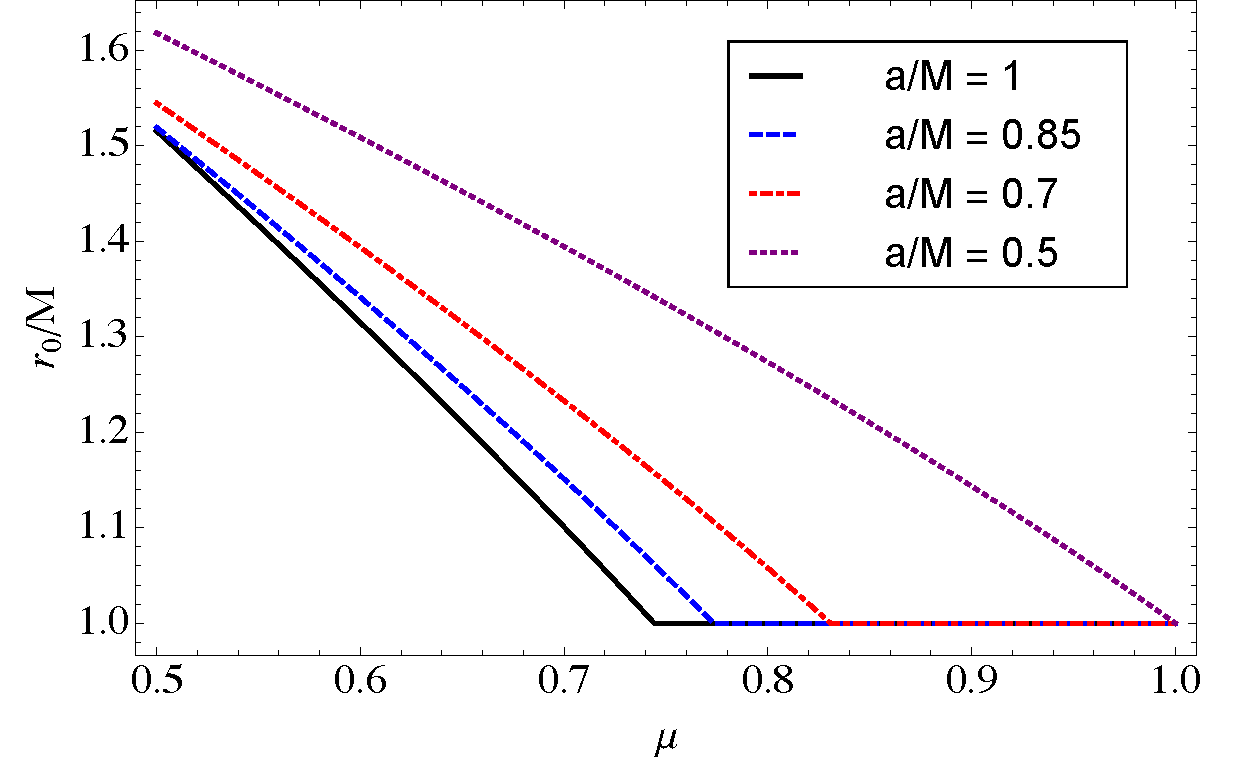
\includegraphics[width = 1.0 \columnwidth]{chapter_extremal/etc/KNPeak} \\
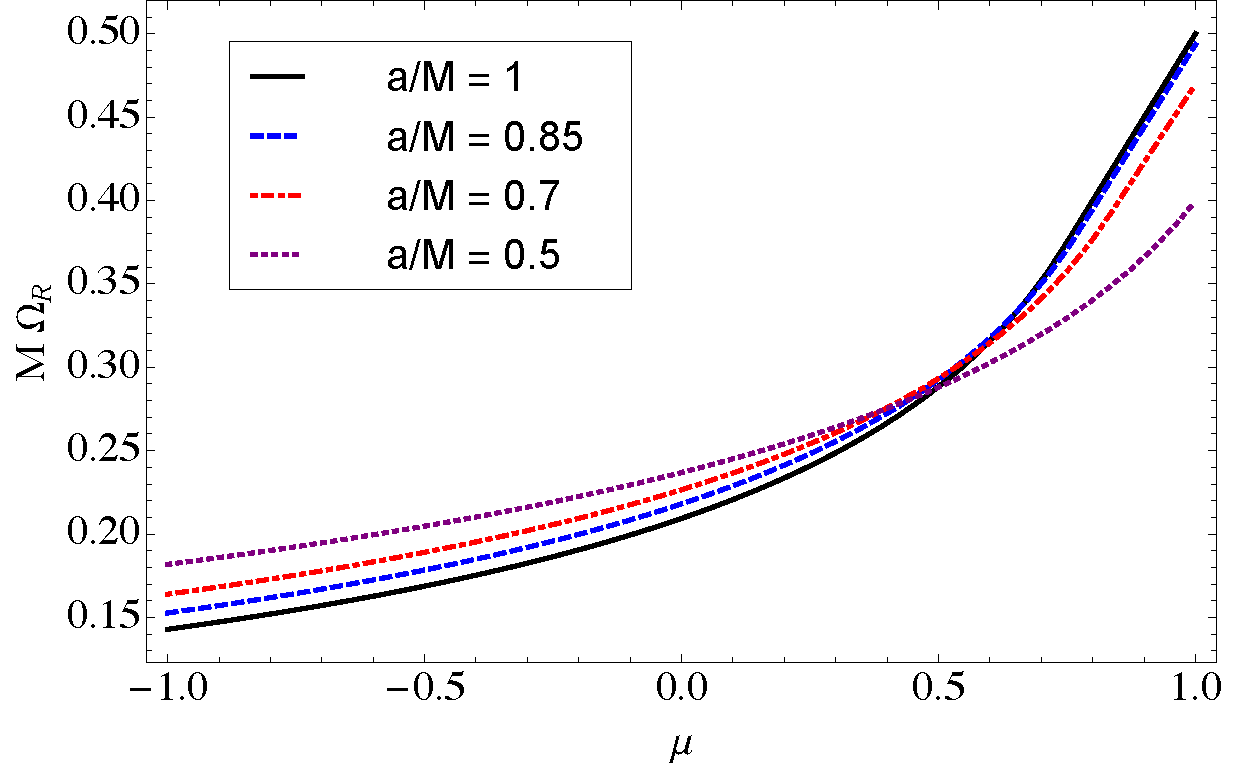
\includegraphics[width = 1.0 \columnwidth]{chapter_extremal/etc/KNOmegaR} \\
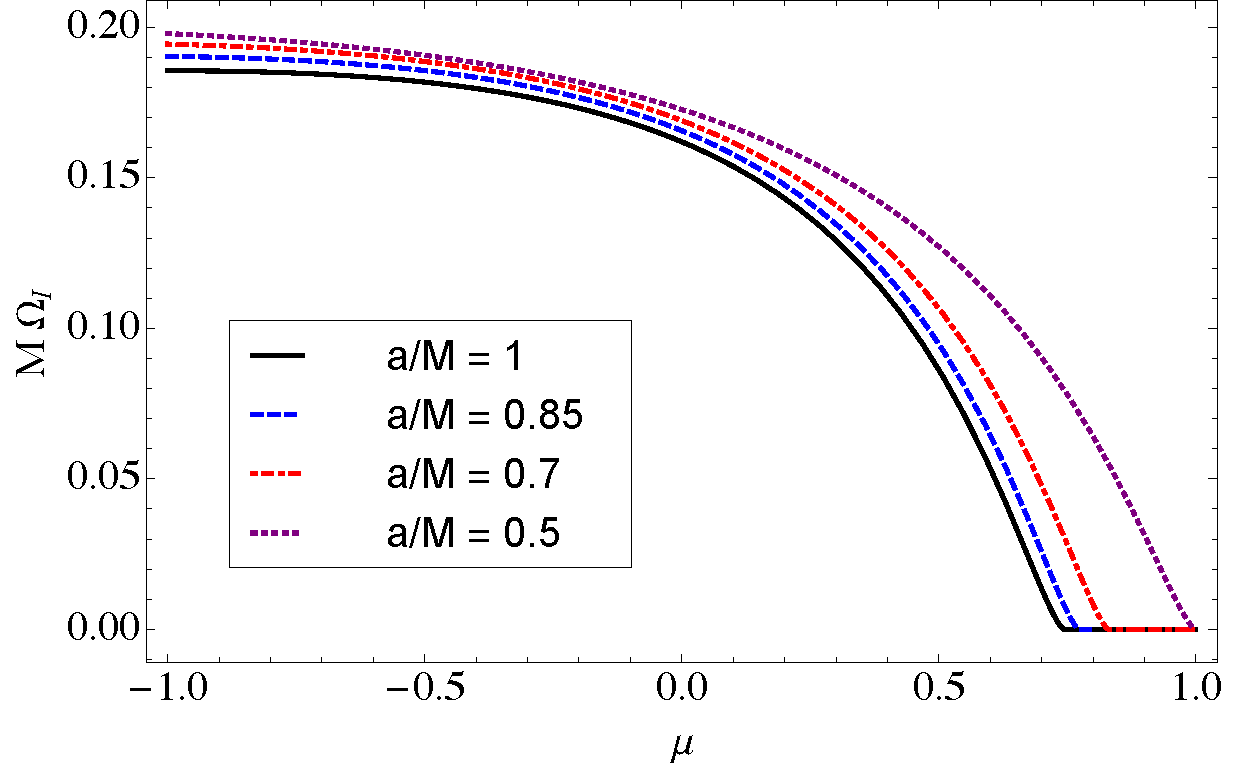
\includegraphics[width = 1.0 \columnwidth]{chapter_extremal/etc/ExKNDecay}
\caption{WKB quantities plotted against $\mu$ for extremal black holes and various values of $a$. {\it Top panel}: The position of the WKB peak $r_0$. {\it Middle panel}: The WKB frequency $\Omega_R$. {\it Bottom panel}: The WKB decay rate $\Omega_I$.}
\label{fig:ExWKB}
\end{figure}


Together with our matching results on the existence of ZDMs for all values of $a$ in the nearly-extremal case, we see the spectrum bifurcation found in Kerr occurs also for the scalar QNMs of KN. 
An important difference between the KN black hole and Kerr is that even when $\mu = 1$, for sufficiently small values of $a$, DMs exist. 
This is expected: extremal RN black holes, where $a=0$, are known to possess damped scalar modes even for $m=l$.

We can derive an approximate formula for the critical $\mu$ above which the WKB results predict ZDMs by investigating the potential $V_u$ in the extremal case. For this, we set $\Omega_R = \mu \Omega_H$. We know that when $a \to M$ (Kerr), a second peak appears outside the horizon for $\mu < \mu_c \approx 0.74$. For KN, $\mu_c$ is a function of $a$. The top panel of Fig.~\ref{fig:CritMu} shows this extremal potential for $\mu =1$ and various values of $a$. We see the second peak emerge when $a < 0.5$ ($Q > \sqrt{3}/2$). With the above simplifications applied to $V_u$ we find that a peak exists outside the horizon when
\begin{align}
\label{eq:ExPoly}
a^2 \mu^2 (r^2 + 2Mr +a^2 +3M^2) - \alpha(M^2+a^2)^2 = 0
\end{align} 
has a solution for $r>M$. Inserting $r=M$ into the above polynomial, we solve for the critical inclination parameter
\begin{align}
\label{eq:MuCrit}
\mu_c^2 = \frac12 \left(3 + \frac{12 - \sqrt{136 +56(a/M)^2 +(a/M)^4}}{(a/M)^2} \right) \,.
\end{align}
This formula was previously given in~\cite{HodEikonal2012,Zhao:2015pqa}, and it it reduces to the known result in Kerr, $\mu_c = [(15 -\sqrt{193})/2]^{1/2}\approx0.74$~\cite{HodEikonal2012,Yang:2013uba}. We plot $\mu_c$ as a function of $a$ in Fig.~\ref{fig:CritMu}. Further setting $\mu_c^2 = 1$ we arrive at the value $a/M = 0.5$ beyond which there are no values of $\mu$ where the WKB peak remains on the horizon.

\begin{figure}[tb]
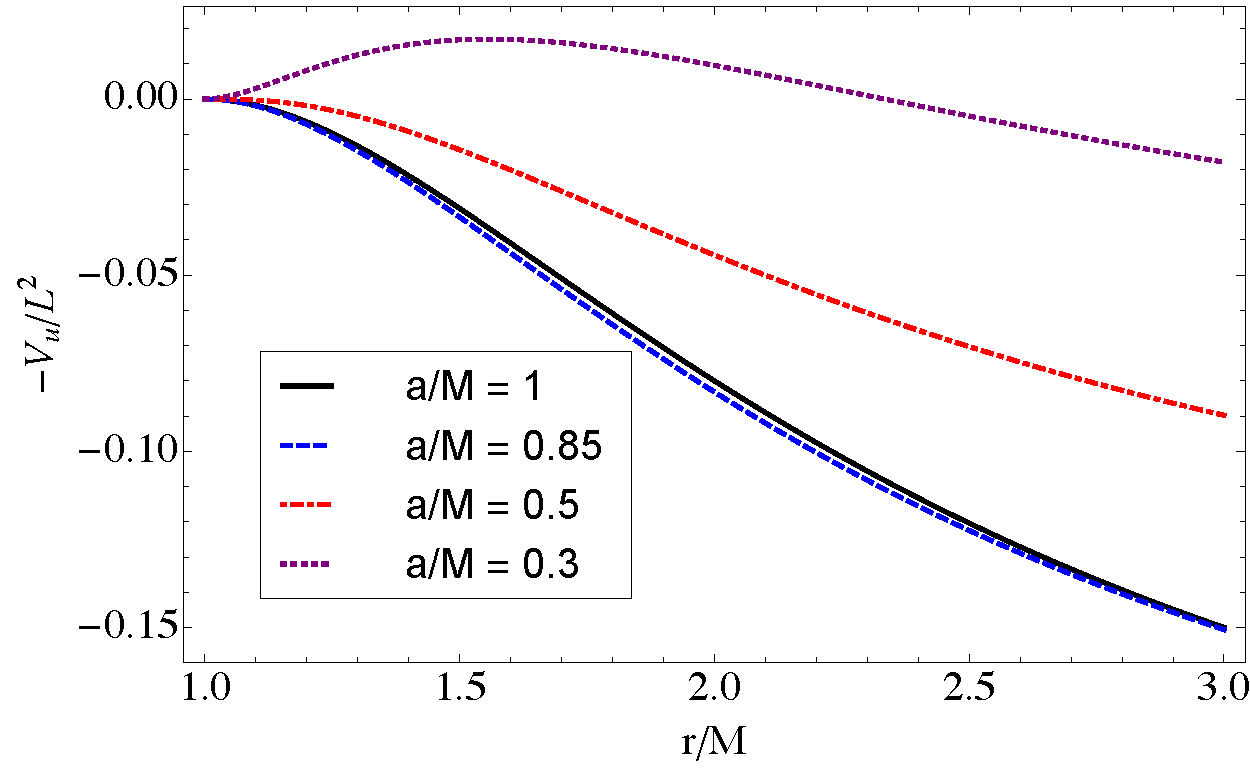
\includegraphics[width = 1.0 \columnwidth]{chapter_extremal/etc/KNEqExPotential}
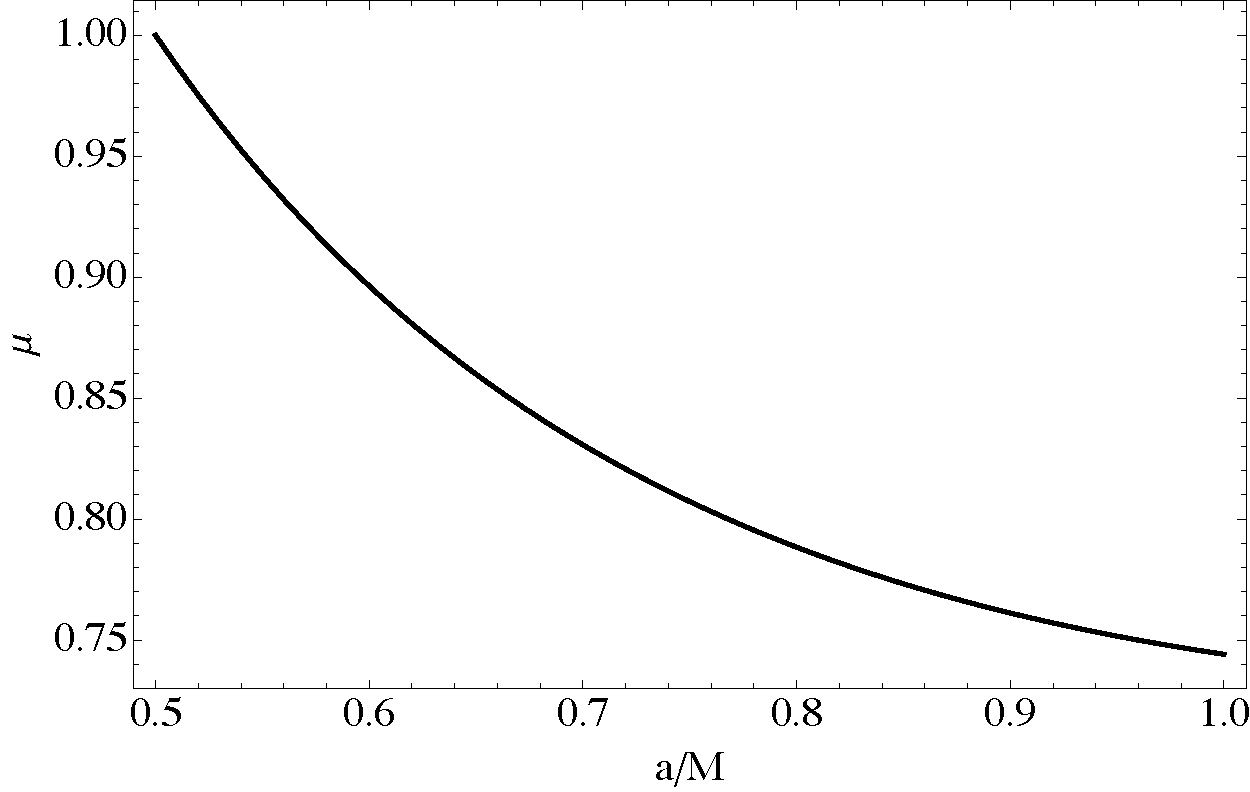
\includegraphics[width = 1.0 \columnwidth]{chapter_extremal/etc/KNCritMu}
\caption{{\it Top panel}: Extremal WKB potential $-V_u/L^2$ plotted for various fixed values of $a$. {\it Bottom panel}: The critical inclination parameter $\mu_c$ below which the extremal potential supports a second peak outside the horizon.}
\label{fig:CritMu}
\end{figure}

We see from this that the nearly-extremal WKB analysis splits into two cases where we expect simple expressions for the frequencies: when the WKB peak is near the horizon and we have ZDMs, and when the WKB peak is supported away from the horizon we have DMs. We briefly treat each case.


\subsubsection{Zero-damped modes}

Now we consider the case where $\sigma \ll1$, and $\mu >\mu_c(a)$. This is the case where we expect that the WKB approximation describes ZDMs. 
Inspired by the form of Eq.~\eqref{eq:ExPoly} and previous work in Kerr, we define
\begin{align}
\mathcal J^2 & = (m \Omega_H)^2(6M^2 +a^2) - A \,,
\end{align}
so that $\mathcal J^2  > 0$ is the condition for $\mu > \mu_c$ in the extremal limit. 
Next, we make the guess that $r_0$ approaches the horizon at a rate controlled by $\sigma$, $r_0 = M( 1+ c \sigma)$.
The solution for the peak at leading order in $\sigma$ is then
\begin{align}
r_0 \approx M\left(1 + \sigma \frac{M m \Omega_H}{\mathcal J} \right) \,.
\end{align}
For this peak, $\Omega_R$ becomes
\begin{align}
\label{eq:WKBOmegaZDM}
\Omega_R \approx \frac{\mu a}{M^2+a^2} - \sigma \frac{M (\mathcal J/L)}{2(M^2+a^2)} \,.
\end{align}
Finally, inserting these results into the expression for $\Omega_I$ gives
\begin{align}
\Omega_I & \approx \frac{M \sigma}{2(M^2+a^2)}\,.
\end{align}
Collecting these, the WKB approximation for $\omega$ is
\begin{align}
\label{eq:WKBFreq}
\omega & = \frac{m a}{M^2 +a^2} - \frac{M \sigma}{2(M^2+a^2)} \left[ \mathcal J + i \left(n + \frac 12 \right) \right]\,.
\end{align}
Equation~\eqref{eq:WKBFreq} for $\omega$ matches the Kerr limit derived in~\cite{Yang:2012he,Yang:2013uba}. 
In addition, it is the correct WKB limit of the ZDM expression~\eqref{eq:DFfreq} since the only difference between $\delta$ and $\mathcal J$ is at subleading order in $L$. 


\subsubsection{Damped modes}
\label{sec:DampedModes}

When the WKB peak is outside the horizon in the extremal limit, the roots of the quartic in the square bracket of Eq.~\eqref{eq:FullExPoly} have involved analytic forms, and the expressions for $\Omega_R$ and $\Omega_I$ do not appear to admit useful simplifications.

The exception is for $\mu = \pm 1$, which gives corotating and counter-rotating orbits, respectively. Due to the symmetries of the QNMs, we focus on the case $\mu = 1$ and allow $a$ to vary between positive and negative values, which interpolates between the two cases as $a$ passes through zero. The position of the peak and corresponding frequency are then
\begin{align}
\label{eq:WKBFreqOuterPeak}
r_0 = 2(M-a)\,, & & \Omega_{\rm peak} =  \frac{1}{4M-3a}\,. 
\end{align}
Here we denote the frequency at the WKB peak $\Omega_{\rm peak}$ to distinguish it from the limiting value $\Omega_H$ when both $\mu = 1$ and the peak is at the horizon. These two limits match smoothly when $a = M/2,$ $Q = \sqrt{3} M/2$.
These give a decay rate
\begin{align}
\label{eq:DMExDecay}
\Omega_I = \frac{(M-2a)\sqrt{2a^2-2Ma +M^2}}{\sqrt{2} (M-a)^2(4M-3a)}\,.
\end{align}
This decay rate joins onto the $\Omega_I = 0$ solution as $a \to M/2$.

\subsection{Numerical results for the Dudley-Finley equation}
\label{sec:DFNumerics}

We turn to the problem of determining the accuracy of our analytic results, Eqs.~\eqref{eq:WKBOmegaI} and \eqref{eq:WKBSolve}, and Eq.~\eqref{eq:DFfreq}, valid in the regime of $L\gg1$ and $\sigma\ll1$ respectively. 
We examine the residual errors in these approximations $\Delta\omega \equiv |\omega_\text{A}-\omega_\text{N}|$, where $\omega_\text{A}$ is computed with the appropriate analytic approximation and $\omega_\text{N}$ is computed numerically with sufficiently small error that we can take $\omega_\text{N}$ to be the ``true'' QNM frequency. 
To numerically compute the QNMs we use Leaver's method \cite{Cook:2014cta, Berti:2005eb, Leaver1985, LeaverRN}. 
Leaver's method turns the coupled eigenvalue problem posed by the radial and angular equations \eqref{eq:TeukR} and \eqref{eq:TeukS} into a root finding problem (see~\cite{Cook:2014cta} for a nice discussion).
The eigenvalues, $\omega$ and $A_{lm}$, are reported as simultaneous roots of two infinite, convergent continued fractions, the values of which we denote $\mathcal C^r$ and $\mathcal C^\theta$:
\begin{align}
\label{eq:cfform}
{\mathcal C^r} = \beta_0^r-\frac{\alpha_0^r\gamma_1^r}{\beta_1^r-}\frac{\alpha_1^r\gamma_2^r}{\beta_2^r- \dots} \,.
\end{align}
The indexed greek letters $\alpha^r_i$, $\beta^r_i$, $\gamma^r_i$ are functions of $\omega$, $A$, $a$, $Q$, $l$, and $m$, and the same equation describes $\mathcal C^\theta$ in terms of $\alpha^\theta_i$, $\beta^\theta_i$, $\gamma^\theta_i$. These functions are given in~\cite{Berti:2005eb}.
To implement Leaver's method, $\mathcal C^r$ and $\mathcal C^\theta$ must be truncated, and the resulting expressions are subjected to a numerical root finding algorithm. 
We use $500+$ terms in the continued fractions and \textit{Mathematica's} FindRoot routine. 
For the purposes of analyzing the accuracy of our analytic formula, we ensure that our numerical errors are orders of magnitude smaller than the errors in the analytic approximations.

\subsubsection{Confirmation of the DF WKB results} \label{sec:WKBnum}

\begin{figure*}[tb]
\label{fig:eikonal}
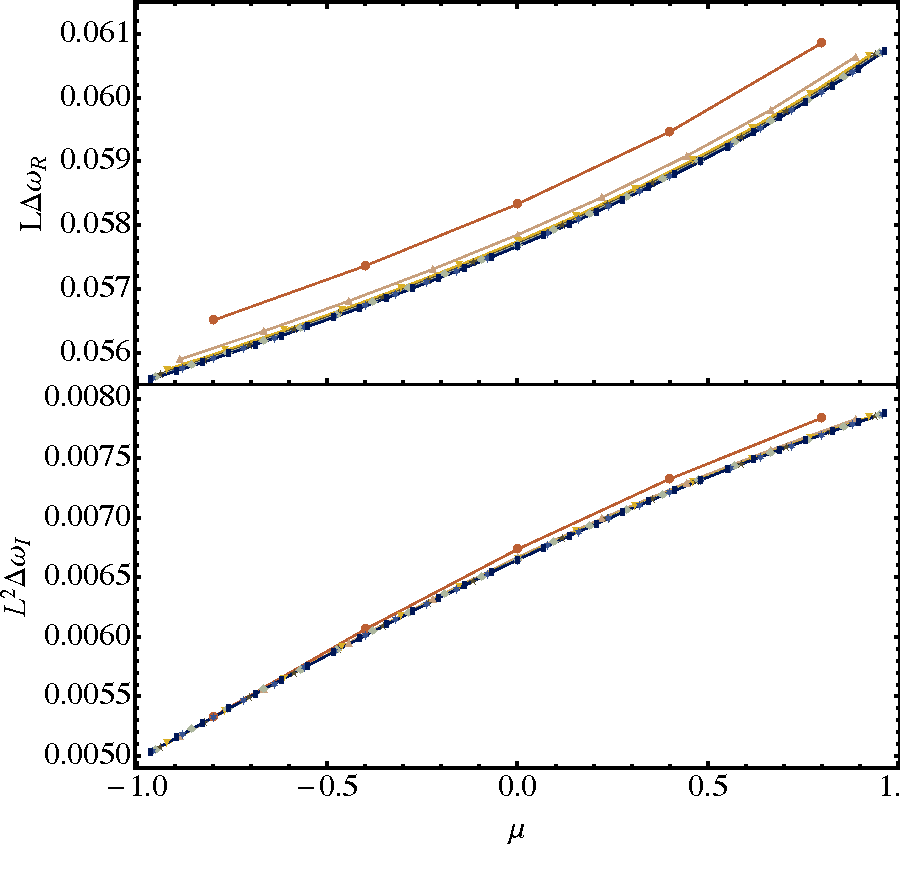
\includegraphics[width =1.0 \columnwidth]{chapter_extremal/etc/eikplot_Q_8_a_2_s_1.pdf}
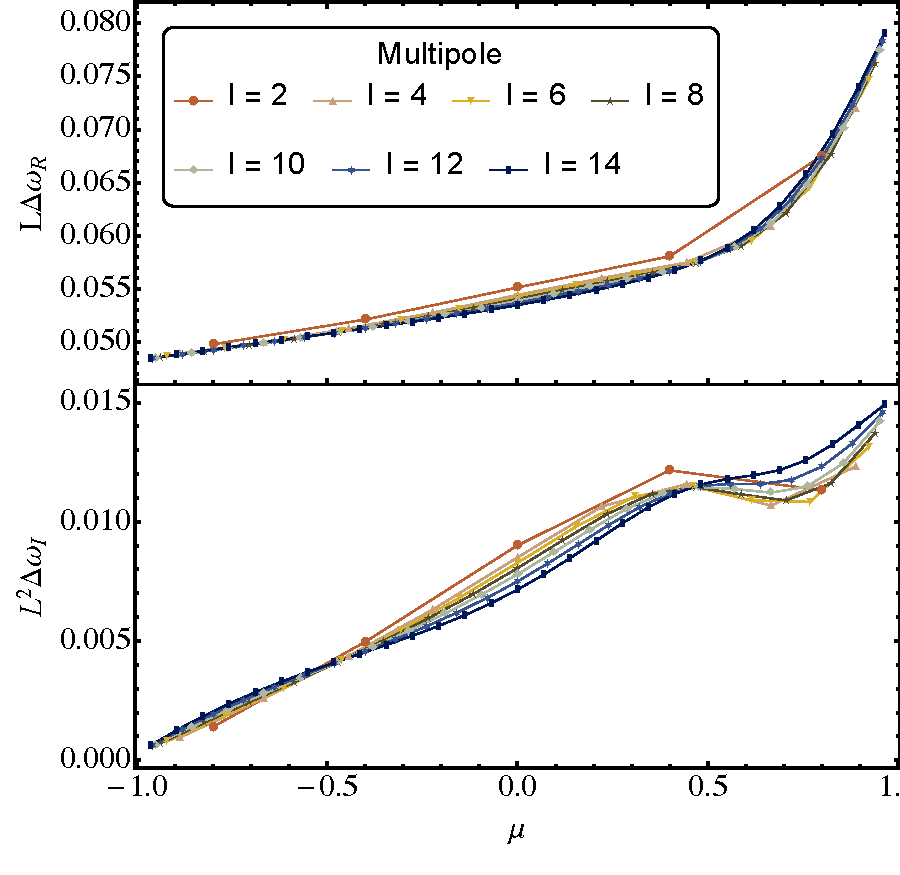
\includegraphics[width =1.0 \columnwidth]{chapter_extremal/etc/eikplot_Q_1_a_9_s_1.pdf} \\
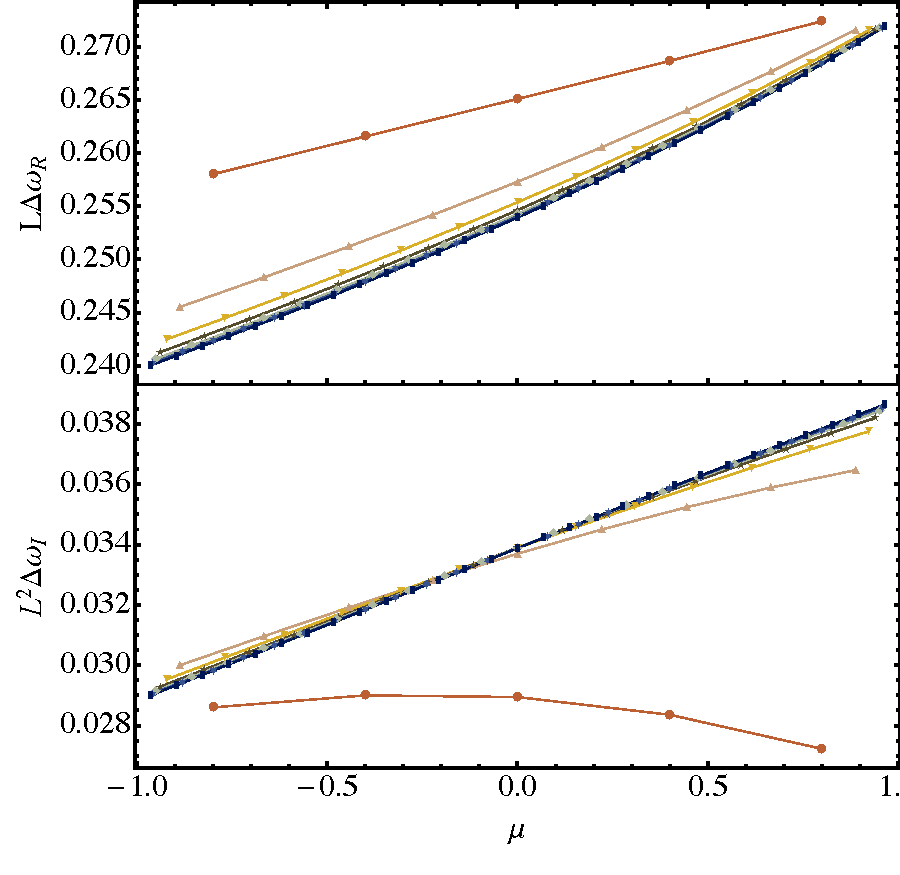
\includegraphics[width =1.0 \columnwidth]{chapter_extremal/etc/eikplot_Q_8_a_2_s_2.pdf} 
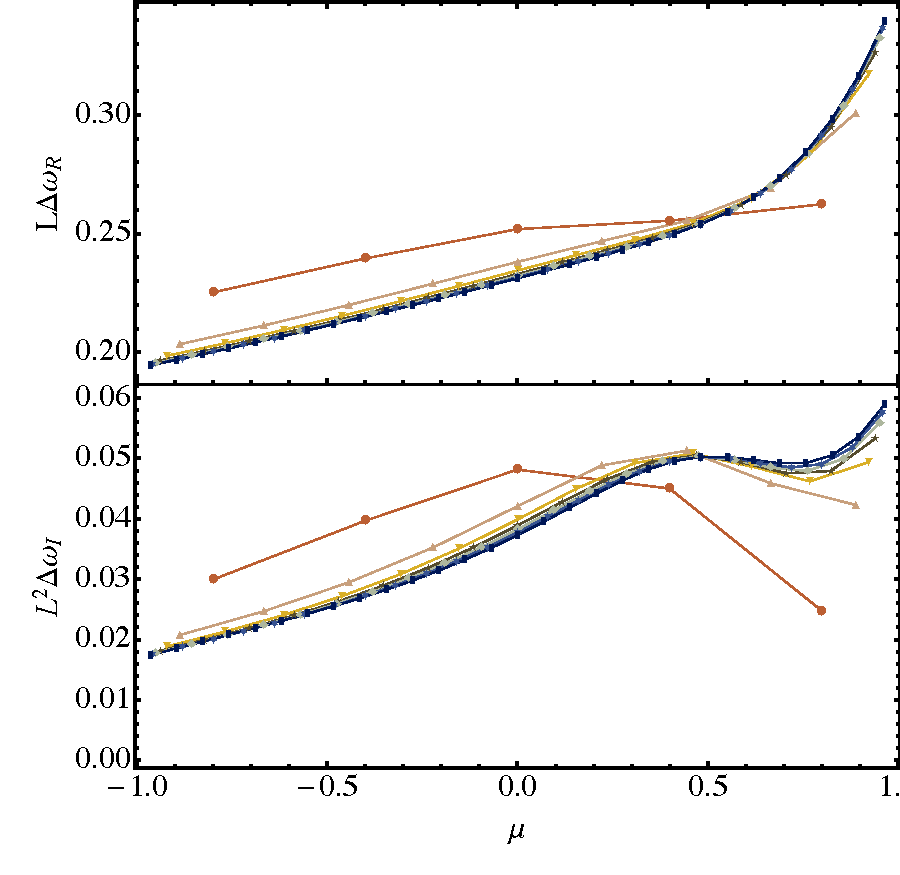
\includegraphics[width =1.0 \columnwidth]{chapter_extremal/etc/eikplot_Q_1_a_9_s_2.pdf}
\vspace{-5mm}
\caption{A numerical study of the error in the DF WKB predictions obtained by solving Eqs.~\eqref{eq:WKBSolve} and~\eqref{eq:WKBOmegaI}. Each panel examines the scaled residual errors $L\Delta \omega_{R}$ and $L^2\Delta \omega_{I}$, for the lowest overtone, using Leaver's method to compute the ``true'' QNM frequency value.
The cases are $Q=0.8M$, $a=0.2M$, $s = 1$ ({\it top left}),  $Q=0.8M$, $a=0.2M$, $s = 2$ ({\it bottom left}), $Q=0.1M$, $a=0.9M$, $s = 1$ ({\it top right}), $Q=0.1M$, $a=0.9M$, $s = 2$ ({\it bottom right}). 
The lines join residuals of constant $l$ and the curves approach a limit curve for every case except  $Q=0.1M$, $a=0.9M$, $s = 1$. For the convergent cases, this indicates the residual error is $O(L^{-1})$ for $\omega_R$ and $O(L^{-2})$ for $\omega_I$. For the case $Q=0.1M$, $a=0.9M$, $s = 1$, the residual errors are still at least $O(1)$ and $O(L^{-1})$, respectively, and are small enough that they may be probing small errors as discussed in Sec~\ref{sec:WKBnum}.}
\label{fig:DFeik}
\end{figure*}

To confirm the WKB predictions for the QNMs of the DF equations, we calculate the analytic $\omega_{\rm A}$ by solving Eqs.~\eqref{eq:WKBSolve} [yielding Eq.~\eqref{eq:WKBOmegaR}] and~\eqref{eq:WKBOmegaI}.
Our closed form expressions assume the approximation for $A_{lm}$ given by Eq.~\eqref{eq:AppxA}. 
When using Leaver's method to find numerical values $\omega_{\rm N}$, we find that seeding the root search at large $l$ is challenging.
To overcome this, we use an accurate approximation for the angular eigenvalue $A_{lm}$ presented in~\cite{Berti:2005gp} (which is especially good at large $l$), leaving only a one-dimensional, numerical root search of $\mathcal C^r$.
In all the cases we have checked, the frequencies calculated in this way are negligibly different than those computed from the coupled root search.

To analyze the error in $\omega_{\rm A}$, we examine modes with $l$ up to $l=14$ for all allowed, discrete values of $\mu=m/(l+1/2)$, with the parameters $Q$, $a$, $s$, and $n=0$ fixed. 
We calculate the scaled residuals $L\Delta \omega_R$ and $L^2\Delta \omega_I$.
These are finite as $L\to\infty$ if $\omega_{\rm A}$ has errors of orders $O(L^{-1})$ and $O(L^{-2})$ in its real and imaginary parts, respectively. 
We join residuals with the same $l$ with lines, so that as $l$ grows the scaled residuals illustrate the limit curve which depends continuously on $\mu$. Four examples are shown in Fig.~\ref{fig:DFeik}, where we increase $l$ from $l = 2$ to $l = 14$.
The parameters for these plots are $s = 1$, $a = 0.2M$, $Q = 0.8M$; $s = 2$, $a = 0.2M$, $Q = 0.8M$; $s = 1$, $a = 0.9M$, $Q = 0.1M$; and $s = 2, a = 0.9M, Q = 0.1M$. We find that the residual errors do generally scale as $\Delta\omega_R = O(L^{-1})$ and $\Delta\omega_I = O(L^{-2})$, which is actually one power of $L$ better than expected by the WKB theory presented in \cite{Schutz:1985zz}. This unexpected accuracy is also seen in Kerr \cite{Yang:2012he}.

It can be difficult to determine visually whether or not the lines are converging to the limit curve.
For the scaling we claim, the spacing between each successive $l$-curve must decrease as they approach the limit curve.
We have checked that this is the true for all the cases in Fig.~\ref{fig:DFeik} except for $s = 1$, $a = 0.9M$, $Q = 0.1M$ (top right panels of Fig.~\ref{fig:DFeik}).
There, the spacing between the curves appears to be small and constant.
The magnitude of the residual errors are ten times smaller than the $s = 2$, $a = 0.9M$, $Q = 0.1M$ case, and we believe it is likely that we are probing errors introduced by using Eq.~\eqref{eq:AppxA} for $A_{lm}$ in the DF WKB implementation, or from using the $A_{lm}$ expansion in the continued fraction $\mathcal C^r$.
Because the residual is quite small, and still an order of $L$ below the leading WKB prediction, we conclude that the WKB formulae here should be accurate enough for most purposes.


\subsubsection{Confirmation of the matched asymptotic expansion results}

\begin{figure*}[t]
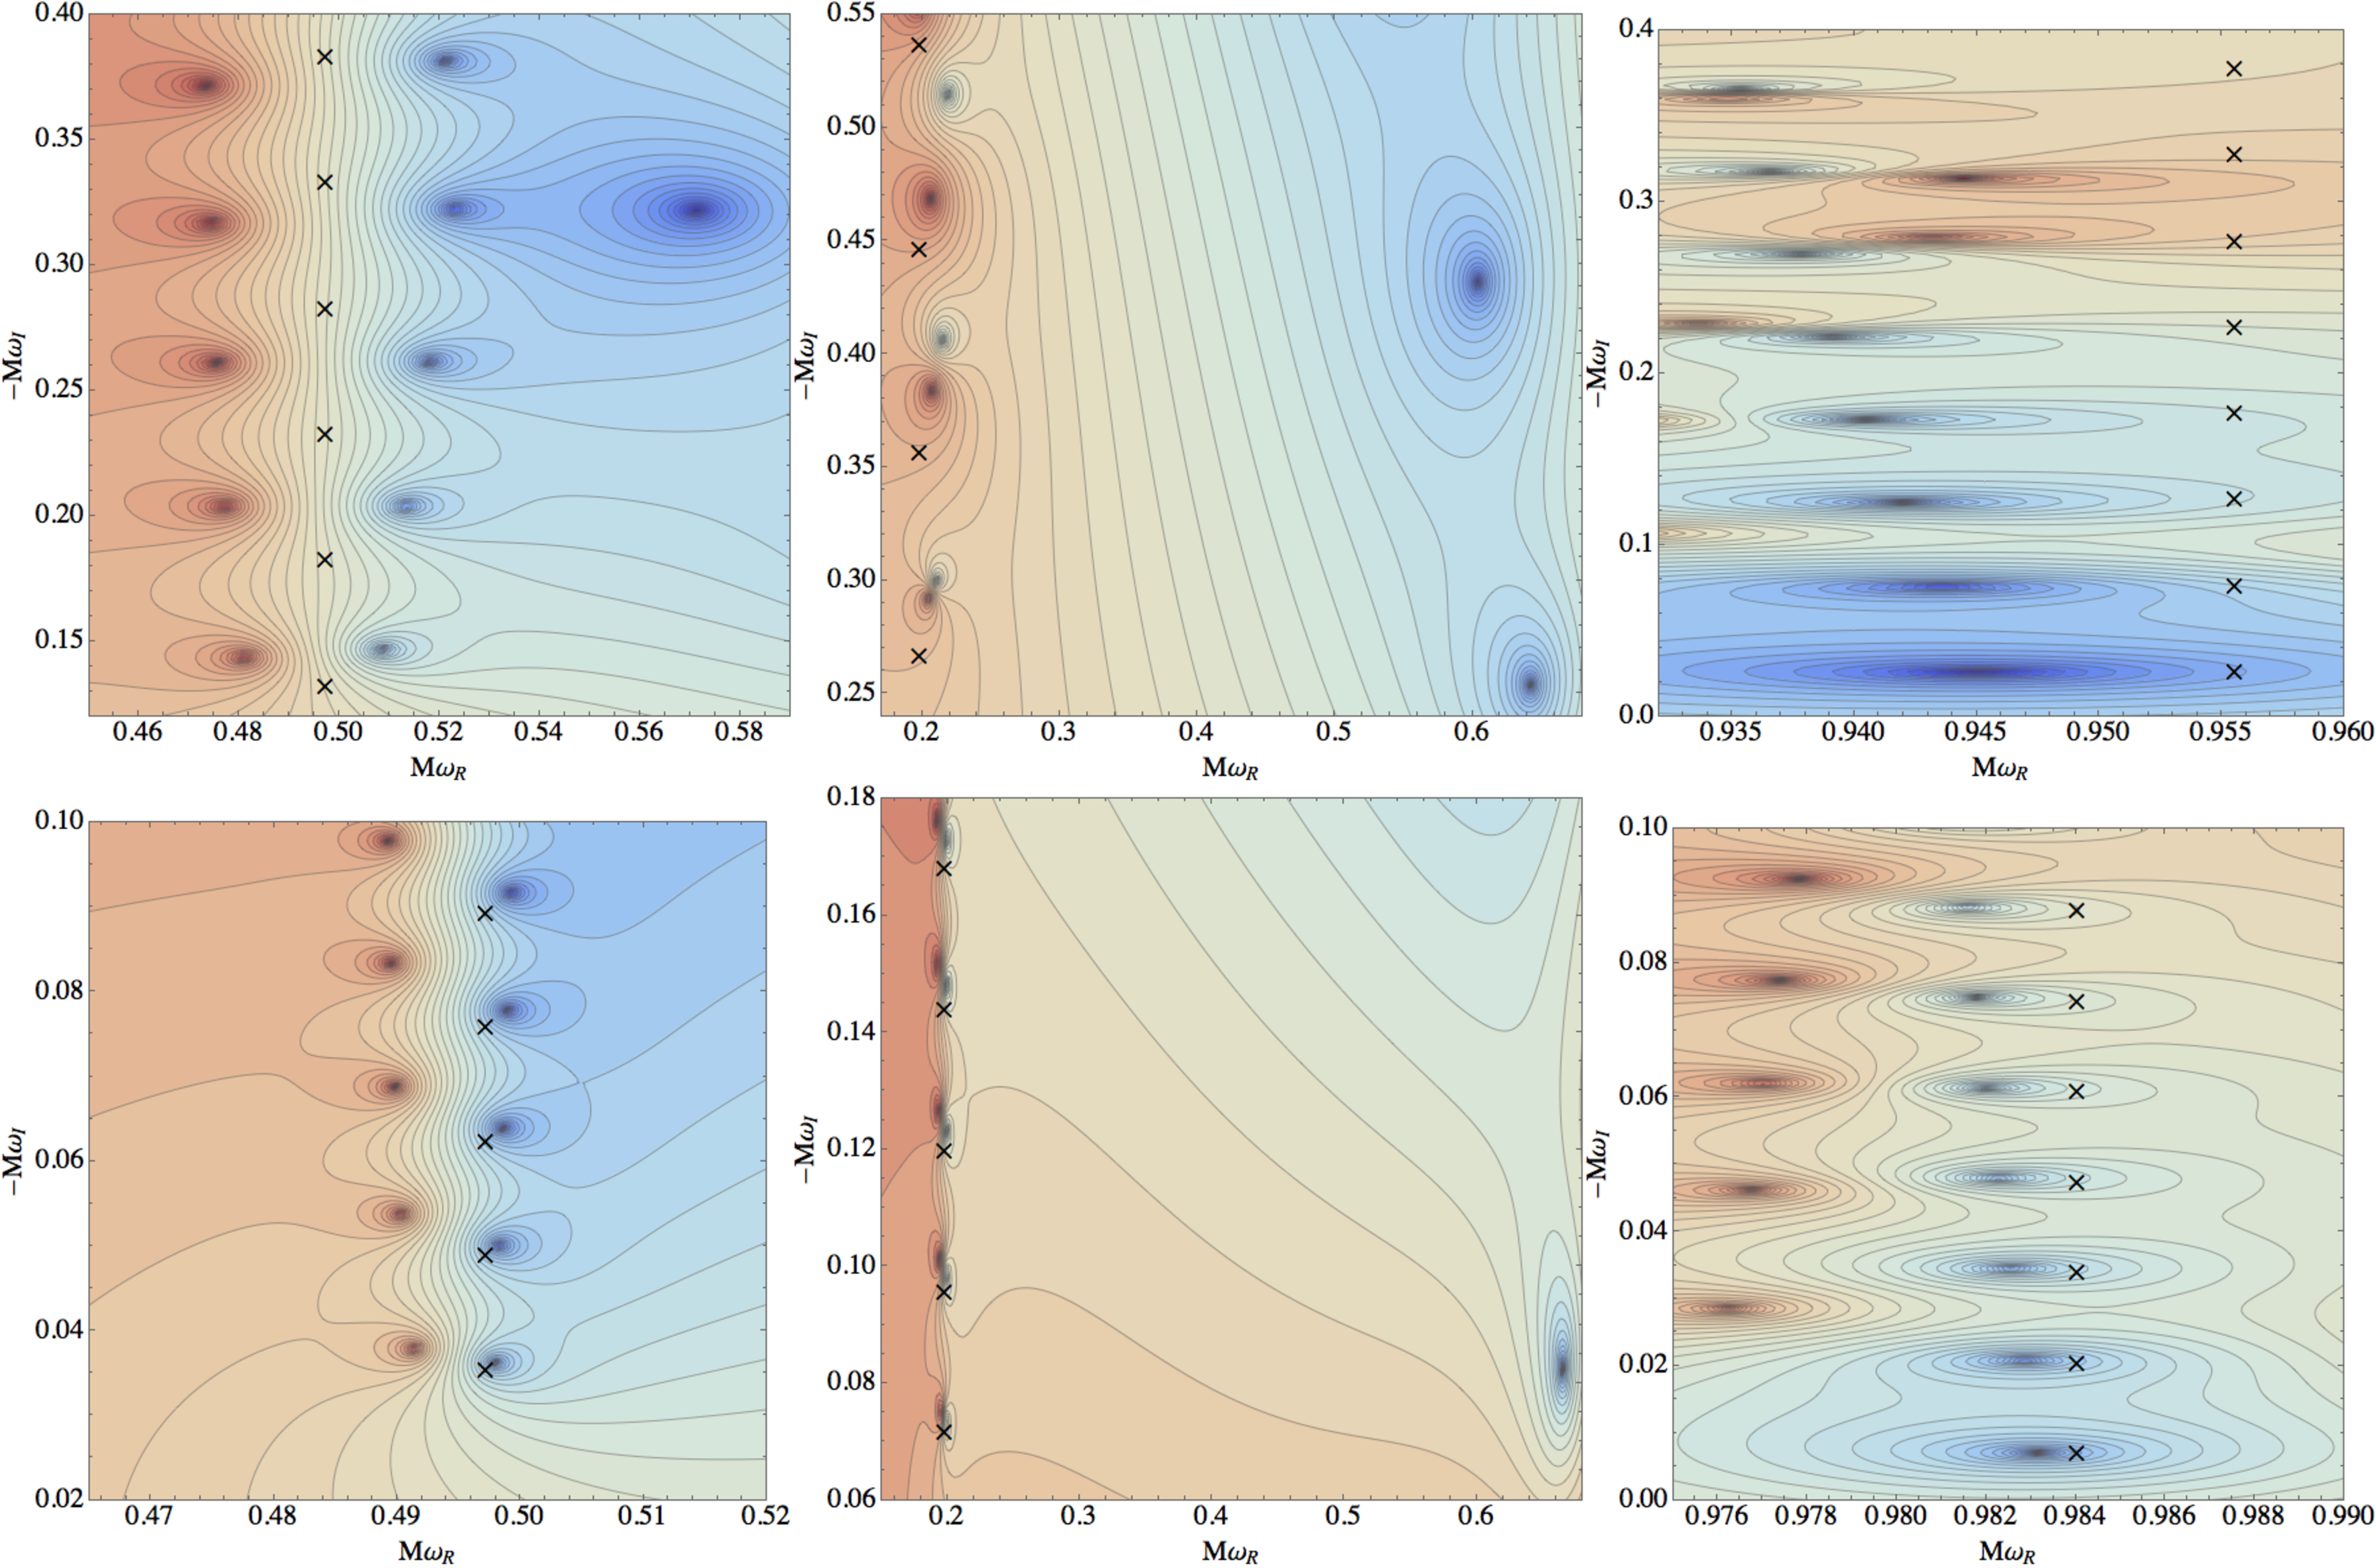
\includegraphics[width = 1.0 \textwidth]{chapter_extremal/etc/CFContourPlotsDF}
\caption{Contour plots of the logarithm of Leaver's radial continued fraction $|\mathcal C^r|$.  Blue (dark) areas correspond to smaller values, and redder (lighter) areas to larger values. The zeros of the continued fraction (seen above as a cluster of contours in a dark region) are QNM frequencies, and are usually accompanied by a pole nearby (a cluster of contours in a lighter region).
The predictions from the matched asymptotic expansion are marked by black crosses.
For the top row of panels, we set $\sigma = 0.182$ and for the bottom row we set $\sigma  = 0.049$. 
{\it Left column}: The case $a = 0.9 M$, $s = 0$, $l=2$, and $m =1$. The zeros appearing in a vertical line with $M\omega_R \approx 0.5 $ correspond to to ZDMs. A damped mode is also visible to the right of the ZDMs in the top panel. In the bottom panel, the ZDMs stack more neatly and have moved closer to the real axis; the DM is outside of the range of the plot.
{\it Center column}: The case $a = 0.1 M$, $s = 0$, $l=2$, and $m =2$. Again, some of the DMs are visible on the right.
{\it Left column}: The case $a = 0.9 M$, $s = 0$, $l=2$, and $m =2$. As $\delta^2>0$, there are no damped modes in the spectrum.}
\label{fig:cfplot}
\end{figure*}

In this section we investigate the scalar ZDMs $(s=0)$ of the KN spacetime and compute $\omega_{\rm A}$ using Eq.~\eqref{eq:DFfreq}, obtained from the matched asymptotic 
expansion\footnote{We note that charged, massive scalar QNMs were investigated using Leaver's method in~\cite{KonoplyaNEKN}. That study provided some results in the massless, uncharged limit, which is the problem we investigate here. However, that study found that in the extremal limit, QNMs which were ZDMs in Kerr limited to a finite decay rate for $Q \neq 0$. This is in conflict with the results we present here.}. 
We verify that the residual error in the analytic formula scales as $\sigma^{2}$, which can be taken as an independent check of the validity of the matched asymptotic calculation. 

In certain regions of parameter space, it can be difficult to apply Leaver's technique because $\mathcal C^r$ becomes a rapidly varying function of $\omega$ and the success of the root-finding scheme becomes heavily dependent on the accuracy of the initial seed. 
We find in practice that this can occur when many QNM frequencies bunch together, which is the qualitative behavior we expect for the ZDMs. To get a sense of where the roots are, we borrow a technique from~\cite{Yang:2012pj} where contours of the logarithm of $|\mathcal C^r|$ are plotted as a function of complex $\omega$. 
QNM frequencies appear as clusters of contours forming circles around places where $\mathcal C^r$ is zero. 
Non-physical poles~\cite{LeaverPoles} of $\mathcal C^r$ also appear as clusters of contours forming circles; however these can be distinguished by examining the value of the continued fraction. 
In our plots, blue (dark) regions correspond to smaller values of $|\mathcal C^r|$, while red (light) regions correspond to  larger values. 

Such plots can immediately demonstrate the existence of separated families of DMs and ZDMs. In these plots we fix $a$, $s=0$, $l$, and $m$, and examine two different values of $\sigma$. The ZDMs appear in a roughly vertical line with $\omega_R \approx m \Omega_H$. In the more extreme case, the line shifts toward the real axis and stacks more neatly, as seen in the left column of Fig.~\ref{fig:cfplot} where $l=2$, $m=1$, and $a = 0.9 M$. DMs can be distinguished in these figures, and move only slightly as $\sigma$ is decreased. A single DM can be seen in the top left panel of Fig.~\ref{fig:cfplot}.

\begin{figure}[tb]
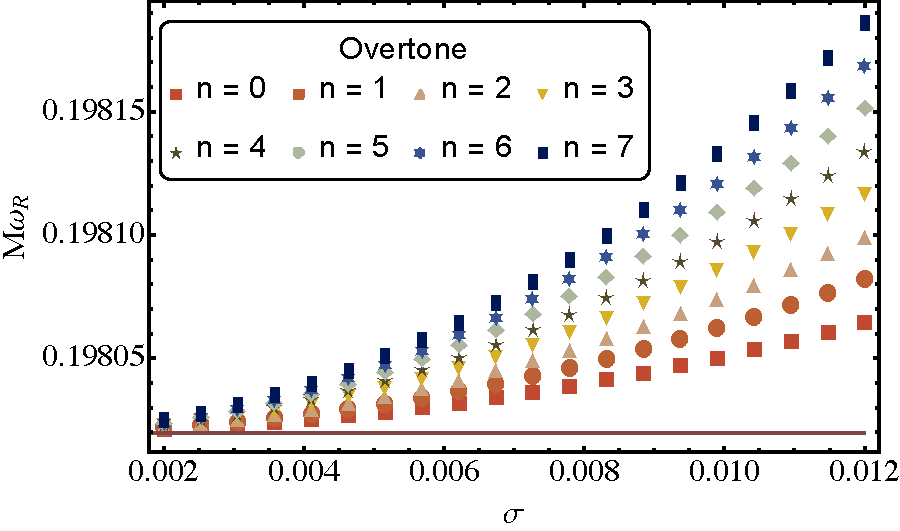
\includegraphics[width =.95 \columnwidth]{chapter_extremal/etc/a1resRe.pdf}
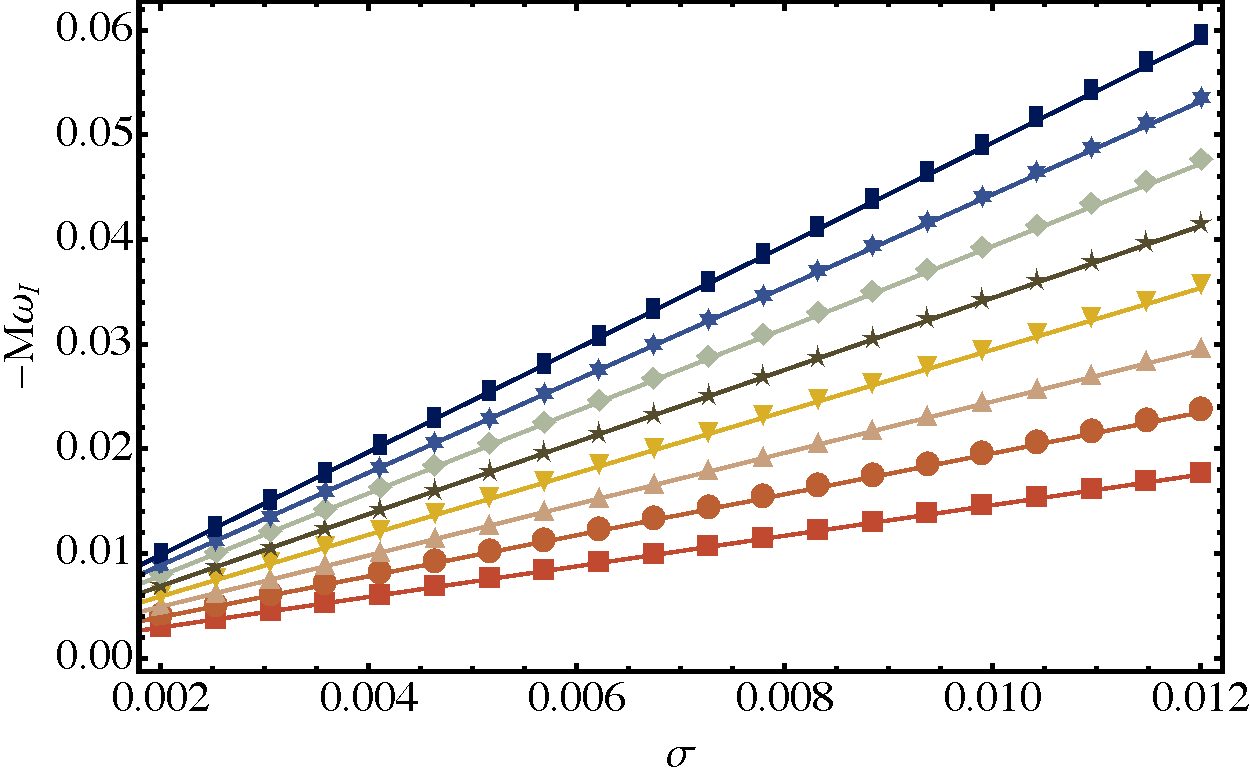
\includegraphics[width =.95 \columnwidth]{chapter_extremal/etc/a1resIm.pdf}
\caption{{\it Top panel}: We fix $a = 0.1 M$, $s=0 $, $l=2$, $m =2$ and study $\omega_R(\sigma)$ when $\delta^2 <0 $. Numerical calculations using Leaver's method appear as points and the analytical prediction is the solid line. The analytical prediction for $\omega_R$ is independent of $n$ and $\sigma$ at order $O(\sigma)$, so that the errors are $O(\sigma^2)$. {\it Bottom panel}: Fixing the same parameters, we study $\omega_I(\sigma)$. 
}
\label{fig:a1res}
\end{figure}


To illustrate the accuracy of our analytic approximations, we fix $s = 0$, $l = 2$ and test Eq.~\eqref{eq:DFfreq} for chosen values of $m$ and $a$. Together with a choice of $\sigma \ll1  $, this fixes $Q$.
Since the QNMs with $\delta^2>0$ are expected to be qualitatively different from those with $\delta^2<0$, we choose a value of $a$ covering each case.
We start with $\delta^2<0$, and examine QNMs with $a = 0.1 M$, $m =2$  while varying $\sigma$. The center column of Fig.~\ref{fig:cfplot} presents the contour plots for two values of $\sigma$, and we observe the qualitative signatures of ZDMs. 
Figure~\ref{fig:a1res} contains a more detailed look at the $\sigma$-dependence of $\omega$ for the eight lowest overtones, and demonstrates the excellent agreement with the analytic formula. 
For the $\delta^2>0$ regime, we fix $a = 0.9 M$ and $m =2$. In Figs.~\ref{fig:cfplot} (right column) and \ref{fig:a9res}, we present the similar plots to Figs.~\ref{fig:cfplot} (center column) and \ref{fig:a1res}, except with $a=0.9M$. Again we observe ZDMs in good agreement with the analytic prediction.


\begin{figure}[tb]
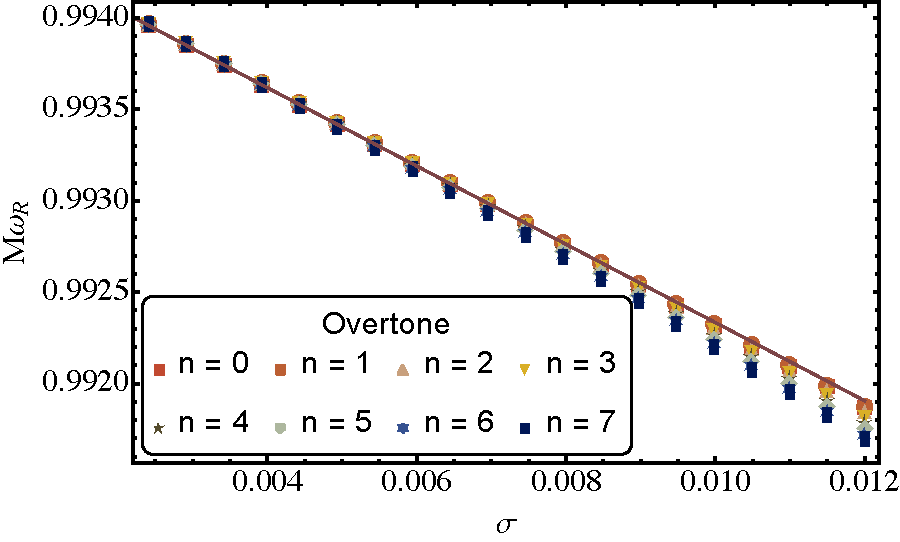
\includegraphics[width =.95 \columnwidth]{chapter_extremal/etc/a9resRe.pdf}
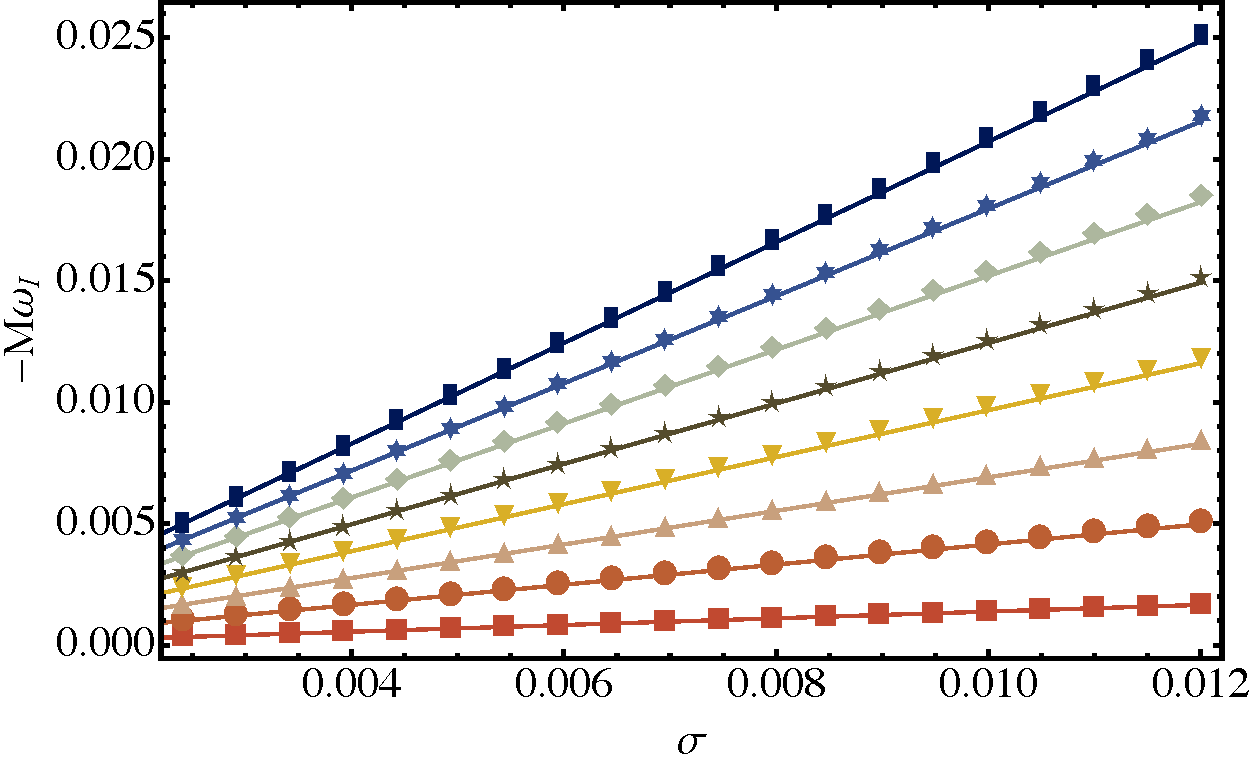
\includegraphics[width =.95 \columnwidth]{chapter_extremal/etc/a9resIm.pdf}
\caption{{\it Top panel}: We fix $a = 0.9 M$, $s=0 $, $l=2$, $m =2$ and study $\omega_R(\sigma)$ when $\delta^2 > 0$. Numerical calculations using Leaver's method appear as points and the analytical prediction is the solid line. Unlike the $\delta^2<0$ case, the analytic prediction for $\omega_R$ now has linear $\sigma$ dependence. {\it Bottom panel}: Fixing the same parameters, we study $\omega_I(\sigma)$.}
\label{fig:a9res}
\end{figure}


We expect the analytic formula to have residual errors of $O(\sigma^2)$. 
Hence we expect the quantity $\sigma^{-2}\Delta \omega$ is $O(1)$ as $\sigma \to 0$, representing the next order in the nearly-extremal expansion. 
In the left panel of Fig.~\ref{fig:DFsigcon}, we return to the $\delta^2 <0$ case $a = 0.1M$, $l = m =2$. We plot the scaled residuals errors $M (n+1/2)^{-1}\sigma^{-2}\Delta \omega$ for the real and imaginary parts of $\omega$ of the lowest eight overtones as we vary $\sigma$.
For each overtone, we can follow the curve from right to left and observe that the scaled residuals become constant, demonstrating $M\Delta\omega = O(\sigma^{-2})$. 
We can also follow the curves from top to bottom and observe that they cluster around a limit curve, indicating $M\Delta \omega=O(n+1/2)$ at large $n$. 

\begin{figure*}[tb]
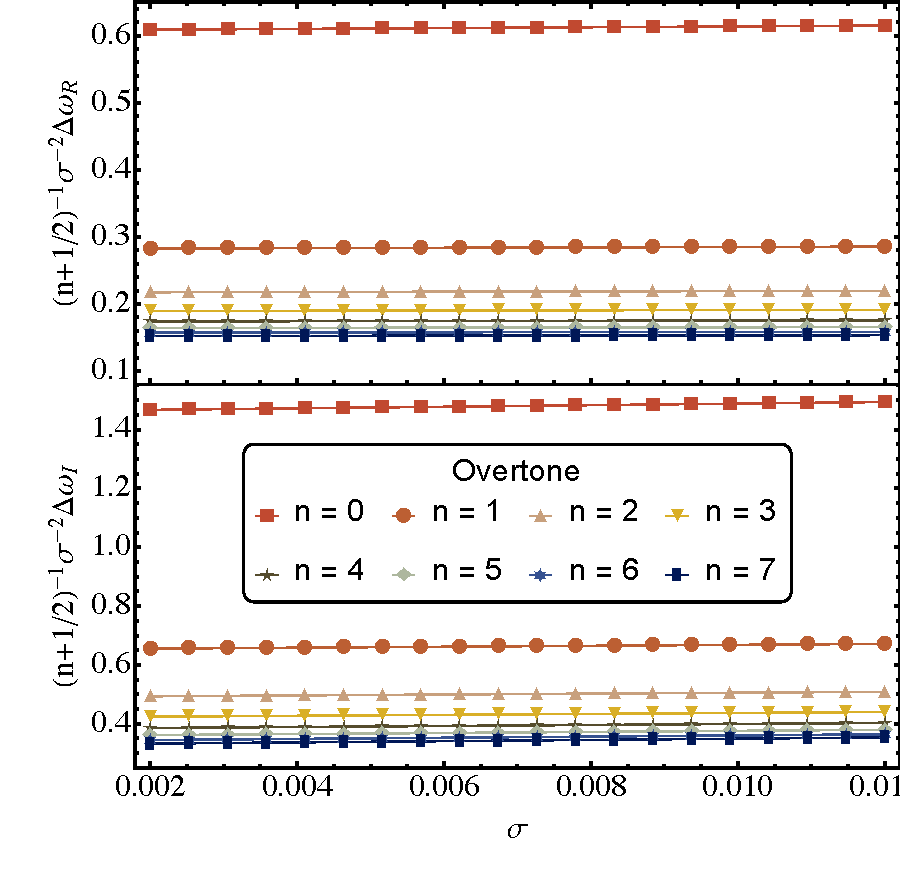
\includegraphics[width =1.0 \columnwidth]{chapter_extremal/etc/sigplot_a_1_s_0.pdf}
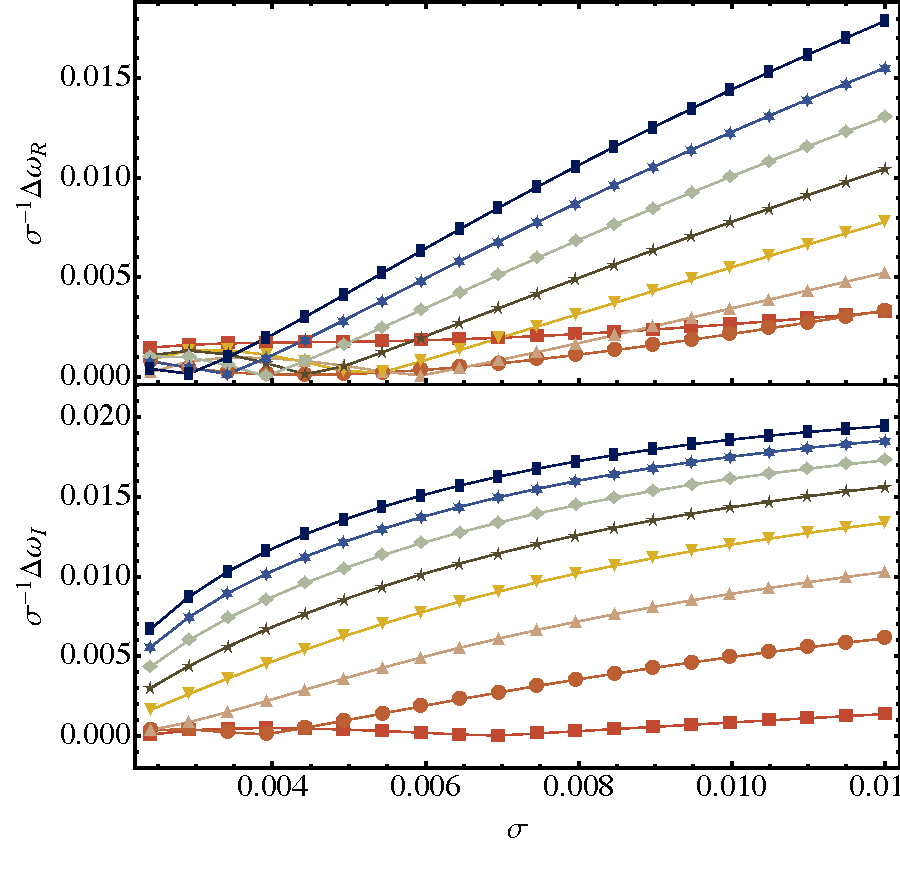
\includegraphics[width =1.0 \columnwidth]{chapter_extremal/etc/sigplot_a_9_s_0.pdf} \\
\vspace{-5mm}
\caption{Scaled residual errors of the $s=0$ ZDM frequencies for the first eight overtones of a KN black hole. 
{\it Left}: We study the $\delta^2<0$ regime and fix $a  = 0.1 M$, $l=2$, $m =2$, letting $\sigma$ vary. We find that the residuals are $O(\sigma^2)$. {\it Right}: We study the $\delta^2>0$ regime and fix $a  = 0.9 M$, $l=2$, $m =2$, letting $\sigma$ vary. The $O(\sigma)^2$ scaling of the residuals ceases to hold at low enough $\sigma$, as discussed in the text.}
\label{fig:DFsigcon}
\end{figure*}

In the right panel of Fig.~\ref{fig:DFsigcon}, we return to the $\delta^2 >0$ case $a=0.9 M$, and $l = m =2$. 
We observe that the residual errors scale are $O(\sigma)$, since the quantity $\sigma^{-1}\Delta \omega$ approaches a nonzero finite number as $\sigma \to 0$.  
In our case studies, all of the modes with $\delta^2 >0$ had residual errors one power larger than the modes with $\delta^2 < 0$ at these small values of $\sigma$.
This indicates that in these cases, where only ZDMs are present, the additional term $\eta$ in Eq.~\eqref{eq:DFfreq} (discussed further in Appendix \ref{sec:MatchingApp}) is not completely negligible, with $\eta \sim 10^{-3}$.
When $\sigma \sim 10^{-3}$, the $O(\eta\sigma)$ correction is not negligible relative to the $O(\sigma^2)$ term in  Eq.~\eqref{eq:DFfreq} and the $O(\sigma^2)$ convergence is not seen.

\begin{figure}[tb]
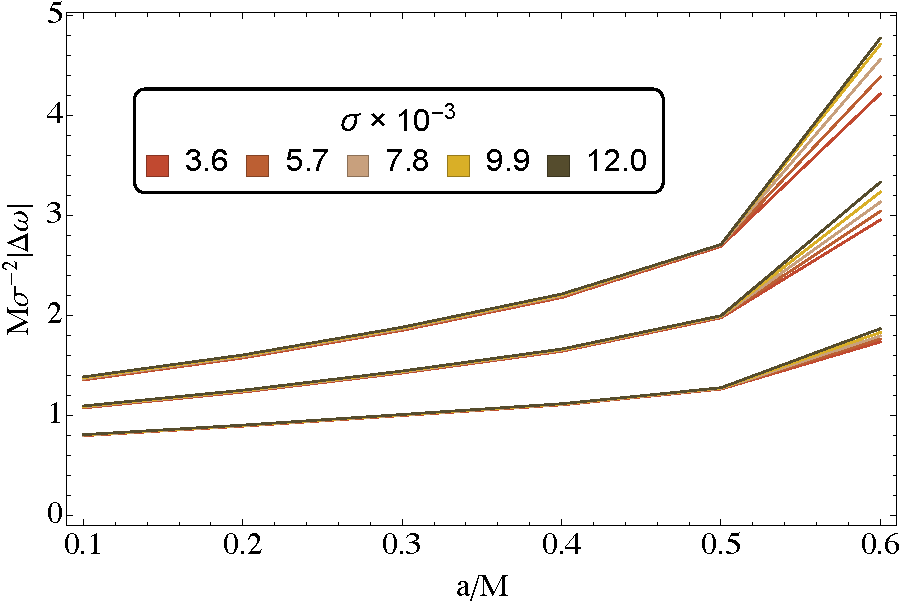
\includegraphics[width =1.0 \columnwidth]{chapter_extremal/etc/sigmaconvergence}
\caption{An evaluation of the convergence of the ZDM frequency formula Eq.~\eqref{eq:DFfreq}. We plot $\sigma^{-2}|\Delta\omega|$ for the three lowest overtones for each of six values of $a$, with $s=0$, $l=2$, $m=2$. In each case, $\delta^2<0$, and $\sigma$ is decreased towards extremality. The overtones are distinguished by the fact that $|\Delta\omega|$ increases with overtone. A finite value of the limit corresponds to following the curves in each overtone band from top to bottom and observing a linear approach to a limit curve. We have checked that the points linearly approach a limit curve for each value of $a$ presented here.}
\label{fig:errscale}
\end{figure}

Meanwhile, in Fig.~\ref{fig:errscale} we show that $\eta$ is so small that $\Delta\omega = O(\sigma^{-2})$ in practice when there are DMs ($\delta^2<0$). 
Here we first fix a value of $a$ and $n$ and calculate  $M (n+1/2)^{-1}\sigma^{-2}\Delta \omega$ for several values of $\sigma$, spaced by roughly $\Delta \sigma \approx 2 \times 10^{-3}$. 
We plot these points in Fig.~\ref{fig:errscale} above the corresponding value of $a$. 
For each of the three overtones, the lines corresponding to the same value of $\sigma$ are plotted with the same color and the limit  $\mathcal \sigma \to 0$ is taken by following the curves from top to bottom. 
We plot the data for six values of $a$, evenly spaced from $a = 0.1 M$ to $a = 0.6 M$, and connect  data points with the same values of $\sigma$ to allow for a rough interpolation to other values of $a$.
The exception is $a = 0.7M$ (not shown), where $\delta^2$ is negative and close to zero, and we expect a larger value of $\eta$. In this case, we find that the residuals do not scale as $\sigma^{2}$.

Overall, the numerical results indicate that the simple expression~\eqref{eq:DFfreq} can be used over a large range of the parameter space. However, care must be taken to include the correction $\eta$ when $\delta^2$ is close to zero, and when the hole is very close to extremality, e.g. $\sigma \sim 10^{-3}$ (when $Q = 0$, $\sigma \sim 10^{-3}$ gives $a/M \sim 1 - 10^{-6}$).


\section{Gravito-electromagnetic modes of Reissner-Nordstr\"{o}m}
\label{sec:RN}

The existence of ZDMs for spin-weighted scalar perturbations of NEKN black holes naturally raises the question of whether ZDMs also exist for gravitational and electromagnetic perturbations of KN.
As discussed previously, the equations for GEM perturbations of KN are coupled, and so electromagnetic perturbations cannot be considered separately from gravitational perturbations.
We can begin to approach this challenging problem by considering first the simpler case of RN.
The results of Sec.~\ref{sec:DF} hold for any spin parameter $a$, including the limit of $a \to 0$, and this shows that even in the well-studied case of the RN black hole, there are scalar ZDMs which reduce to zero decay in the extremal limit $Q \to M$.
In this section, we examine the separated, decoupled GEM equations in the NERN background, and show that ZDMs exist for these perturbations as well.

The ZDMs of RN are purely decaying, like the $m=0$ ZDM modes of Kerr and the DF equation, and so they do not fit with the usual intuition into the nature of QNMs. 
Purely decaying perturbations of Schwarzschild have been discussed by Price~\cite{Price:1971fb,Price:1972pw,wheeler1972magic}, although the connection between this exponential decay and quasinormal modes remains unclear.
Purely decaying modes in RN have been described in~\cite{Andersson:1996xw,Andersson:2003fh}, and include the algebraically special modes~\cite{Chandra:1984a}, but to our knowledge none of these exhibit the slow decay rate we find, despite a large literature exploring the QNMs of extremal and nearly-extremal RN black holes~\cite{LeaverRN,Onozawa:1995vu,Berti2009}.
Before exploring the existence of ZDMs for the NERN black hole, we review the fundamental equations for the perturbations of this spacetime.

\subsection{Perturbations of Reissner-Nordstr\"{o}m}

The problem of GEM perturbations for the RN spacetime closely parallels the investigation of perturbations of Schwarzschild using the Regge-Wheeler-Zerilli equations. 
The equations come in two sets, according to the parity of the perturbations, and it is known that the QNM spectrum of both sets is the same~\cite{ChandraBook,Dias:2015wqa}. 
This means that we can focus on the magnetic-parity perturbations [those which are multiplied by $(-1)^{l+1}$ under a parity transform]\footnote{We follow the convention of~\cite{Zerilli:1970wd}. Other studies refer to these modes as odd-parity and even-parity, or axial and polar, see e.g.~\cite{Pani:2013ija,Pani:2013wsa}.}, which gives two equations indexed by $j,k = 1,2$:
\begin{align}
\label{eq:RNwave}
\frac{d^2 Z_j}{dr_*^2}& + (\omega^2 - V_j) Z_j = 0 \,, \\
\label{eq:RNpot}
V_j & = \frac{\Delta}{r^5}\left[ l(l+1) r - q_k +\frac{4 Q^2}{r} \right] \,,
\end{align}
where $q_k$, $k \neq j$ indicates that $q_2\, (q_1)$ be used for $Z_1\, (Z_2)$, and
\begin{align}
q_1 &= 3 M  + \sqrt{9 M^2 +4 Q^2 [l(l+1)-2]} \,, \\
q_2 & = 6M - q_1 \,.
\end{align}
When $Q \to 0$, $Z_1$ obeys the equations for  magnetic-parity electromagnetic perturbations and $Z_2$ obeys the Regge-Wheeler equation for gravitational perturbations. In the above equations, $r_*$ and $\Delta$ are defined in the same way as in the KN spacetime, in the limit $a \to 0$. In particular, $\Delta$ has two roots which give the coordinate positions of the outer and inner event horizons, $r_\pm = M \pm M \sqrt{1 - Q^2/M^2}$.
We are interested in the nearly-extremal limit, where $\sigma = (r_+ - r_-)/r_+ \ll 1$. We maintain the same notation as in Sec.~\ref{sec:DF}, which highlights many parallels between two analyses.

To search for ZDMs in the NERN spacetime analytically, we repeat the steps of the matched asymptotic expansion used for the DF equation in Sec.~\ref{sec:DF}. First we discuss the inner solution.

\subsection{The inner solution}

In the near-horizon, nearly-extremal limit [$x = (r-r_+)/r_+\ll 1$ and $\sigma \ll 1$, but without assuming that $\sigma/x$ is small], Eqs.~\eqref{eq:RNwave} and~\eqref{eq:RNpot} reduce at leading order to 
\begin{align}
y^2 & Z_j''(y) + y Z_j'(y) + V^y_j Z_j (y)= 0\,, \\
V^y_j & = \left(\frac{\hat \omega}{\sigma}\right)^2 +\frac{y[q_k /M -4 - l(l+1)]}{(1-y)^2} \,.
\end{align}
We recall the variable $y$ used in Sec.~\ref{sec:DF}, 
\begin{align}
y = \exp \left( \frac{\sigma r_*} {r_+} \right) \approx \frac{x}{x+\sigma} \,,
\end{align}
By making the replacements $  \hat \omega/\sigma= \varpi / 2 $ and
\begin{align}
 q_k /M -4 - l(l+1) & = \delta_j^2 + 1/4 \,, 
 \end{align}
we see that the near-horizon approximation for $Z_j$ reduces to the same equations as in the DF analysis, Eqs.~\eqref{eq:NHdiffeq} and~\eqref{eq:Ypot}, with $\zeta = 0$, $s = 0$, and 
\begin{align}
\delta_j & = i \left [L + (-1)^{j-1} \right]\,, &&  j  = 1,2\,,
\end{align}
recalling that $L = l+ 1/2$.
Note however that the form of $\delta_j$ differs slightly from the factor $\delta$ for the DF equation in the $a \to 0$ limit. 
In that case, $\delta = i L$ (and is independent of the spin $s$ of the test scalar field). 
For RN, $\delta_j$ is purely imaginary, and we take as our convention that $\delta_j$ is a positive imaginary number.
Again selecting the solution to Eq.~\eqref{eq:NHdiffeq} which has no waves emerging from the horizon and normalizing the amplitude of the solution to unity at the horizon, we have
\begin{align}
\label{eq:RNnearsln}
Z_j & = y^{- i \varpi} (1 - y)^{1/2 + i \delta_j} \, {}_2 F_1\left(\alpha,\beta,\gamma, y \right) \,, \\
\alpha & = 1/2 - i \varpi + i \delta_j \,, \qquad \beta = 1/2 + i \delta_j, \qquad \gamma = 1 - i\varpi \,.
\end{align}
As with the DF equation, we next wish to match this solution onto a solution in the outer region, where $x \gg \sigma$.

\subsection{Ansatz for matching}

We turn to the approximation of Eq.~\eqref{eq:RNwave} when we can take $(x + \sigma) \approx x$. 
Substituting in our definitions, we have after some manipulation,
\begin{align}
&x^2 \frac{d^2 Z_j}{dx^2} + \frac{2x}{(x+1)} \frac{d Z_j}{dx} \notag \\ & + \left[\frac{(x+1)^4}{x^2}  \omega^2 - l(l+1) + \frac{q_k}{x+1} + \frac{4}{(x+1)^2}\right] Z_j  = 0 \,,
\end{align}
We have not yet found a simple analytic solution that gives a convenient matching condition for small $x$. Using transformations such as $Z_j = \Delta^{s/2} r R$ yields promising forms of the equation for various choices of $s$, but none which allow for a straightforward matching analysis. 

Instead, motivated by past experience, we make an ansatz to complete the matching. By expanding the inner solution as in Sec.~\ref{sec:Matching} and Appendix~\ref{sec:MatchingApp}, we have
\begin{align}
\label{eq:RNmatch}
Z_j \to &\frac{\Gamma(2 i \delta_j) \Gamma(1-i \varpi)}{\Gamma(1/2 + i \delta_j)\Gamma(1/2 - i \varpi + i \delta_j)} \left( \frac{\sigma}{x} \right)^{1/2-i\delta_j}\notag \\
&+ (\delta_j \to - \delta_j) \,,
\end{align}
In the case of the DF equation in NEKN, the ZDM solutions correspond to the near-vanishing of one of the two coefficients of $(\sigma/x)^{1/2 \pm i \delta}$ in the above expansion. This occurs at the zeroes of one of the $1/\Gamma(w)$ factors, since $\Gamma(w)$ has poles at the negative integers. We make the ansatz that the corresponding Gamma function is also near its pole in RN. Investigating Eq.~\eqref{eq:RNmatch}, it is apparent that for the convention where $\delta_j$ is a positive imaginary number, the only possibility for fulfilling this criteria here is by taking 
\begin{align}
\label{eq:RNprematch}
1/2 - i \varpi - i \delta_j = - n \,,
\end{align}
which gives 
\begin{align}
\label{eq:RNfreq}
\omega = -i \frac{\sigma}{2r_+} \left[ |\delta_j| + \left(n + \frac 12 \right)\right] \,.
\end{align}
The fact that $\delta_j$ is pure imaginary indicates the presence of DMs in addition to the ZDMs with frequencies given by Eq.~\eqref{eq:RNfreq}, which is of course what is observed. 
These DMs are the usual QNMs of extremal and nearly-extremal RN which have been the subject of past study.

We can provide a heuristic argument in support of our ansatz. 
When $x \gg \sigma$ and $x \lesssim 1$, the two terms in the wave function~\eqref{eq:RNmatch} have distinctly different behavior while approaching the edge of the near-horizon region (corresponding to a decreasing $\sigma/x$). 
In the first term, displayed explicitly in Eq.~\eqref{eq:RNmatch}, $\sigma /x$ has an exponent  $1/2 + |\delta_j| >0$ and so is decaying as $x$ increases. In the second term, where the first term has the replacement $\delta_j \to - \delta_j$, the exponent of $\sigma/x$ is negative and so the term is growing. 
Our matching condition sets this growing term to zero, which is reasonable: when $x \sim 1$, the growing term will have a size $\sim (1/\sigma)^{|\delta_j| -1/2} \gg 1$. 
In the DF case, if the amplitude of this term is not suppressed, this term is too large to match onto the outer solution. 
It seems reasonable that in general an outer solution, which is regular as $\sigma \to 0$, cannot match onto this growing term if the amplitude is not suppressed.
Unless the perturbations have nearly zero amplitude in the near-horizon region, we would encounter unnaturally strong perturbations in the matching region, invalidating the approximate formalism even for QNMs sourced by small initial data.
At the very least, a large amplitude in the matching region goes against the intuition that the ZDMs are concentrated or trapped near the horizon \cite{Andersson2000}. 
This possibility can be avoided for frequencies which eliminate this troublesome growing term.


Note that if an outer solution were available to us, we would find that Eq.~\eqref{eq:RNfreq} is corrected by a small $\eta$ as in the case of the ZDM frequencies predicted by the DF matching analysis of Sec~\ref{sec:DF}. 
This correction would mean that the second term of Eq.~\eqref{eq:RNmatch} is not precisely zero, but its large size is compensated by the small amplitude factor. 
The balance of these two effects would allow for a matching onto the outer solution to take place, as is done for the DF equation.

In Sec.~\ref{sec:RNNumerics} we show that Eq.~\eqref{eq:RNfreq} gives the correct decay rates for the RN ZDMs. 
The fact that this equation differs from the $a \to 0$ limit of the DF prediction, Eq.~\eqref{eq:DFfreq} (recalling that $\delta_j \neq \delta$) shows that the DF equation fails to describe the QNMs of the nearly-extremal RN spacetime outside of the scalar case. 
This is in contrast to the situation where the charge of the NEKN spacetime is small, where the DF equation provides the leading frequency corrections to the Kerr ZDMs~\cite{Mark:2014aja}, and shows that we cannot hope that the DF equation is accurate for all NEKN black holes.

\subsection{WKB Analysis}

For completeness, we include the WKB analysis of Eqs.~\eqref{eq:RNwave} and~\eqref{eq:RNpot}. The form of Eq.~\eqref{eq:RNwave} allows us to immediately use the methods of~\cite{Schutz:1985zz,IyerWill1987}. We recall our definitions $L = l + 1/2 \gg 1$, $\Omega_R = \omega_R/L$, and in the notation of~\cite{Schutz:1985zz} we define
\begin{align}
\mathcal Q = \omega^2 - V_j \approx L^2 \left(\Omega_R^2 - \frac{\Delta}{r^4} \right) \,.
\end{align}
The conditions that $\mathcal Q = 0$ and $d \mathcal Q/dr_* = 0$ at the WKB frequency identifies the peak $r_0$ and gives $\Omega_R$,
\begin{align}
r_0 & = \frac 12 \left( 3 M + \sqrt{9 M^2 - 8 Q^2}\right) \,, &
\Omega_R & = \left. \frac{\sqrt{\Delta}}{r^2} \right|_{r_0} \,,
\end{align}
The curvature at the extrema of the potential determines the decay rate of the mode, Eq.~\eqref{eq:WKBOmegaI}. The result for RN is
\begin{align}
\Omega_I = \frac{\sqrt{3 M^2 r_0 - Q^2 (M+2r_0)}}{r_0^{5/2}}  \,.
\end{align}
These results agree with the literature~\cite{Kokkotas:1988fm,Andersson:1996xw,Mashhoon1985,Cardoso2009}. In the extremal limit,
\begin{align}
r_0 &= 2 M \,, & \Omega_R & = \frac{1}{4M} \,, & \Omega_I & = \frac{1}{4M \sqrt{2}}\,. 
\end{align}
In the context of this study, the important point is that the decay rate remains nonzero for all $Q$, and so this analysis can approximate only the usual DMs of RN in the extremal limit. It does not access the ZDMs.

\subsection{Numerical results}
\label{sec:RNNumerics}

\begin{figure}[tb]
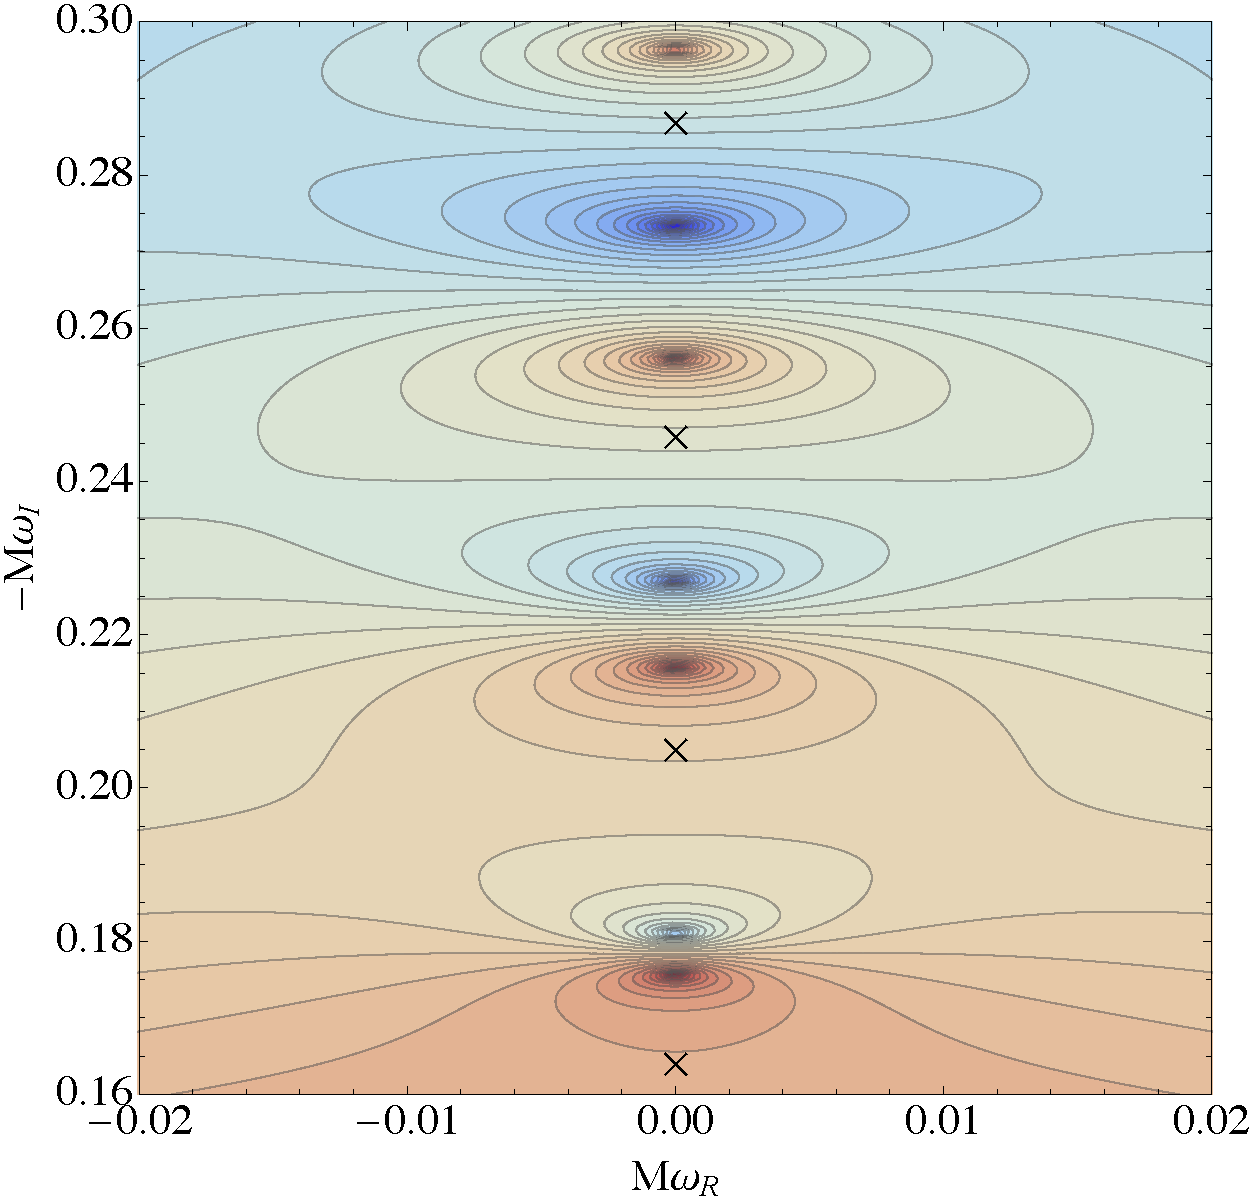
\includegraphics[width =.95 \columnwidth]{chapter_extremal/etc/RNlow.pdf}
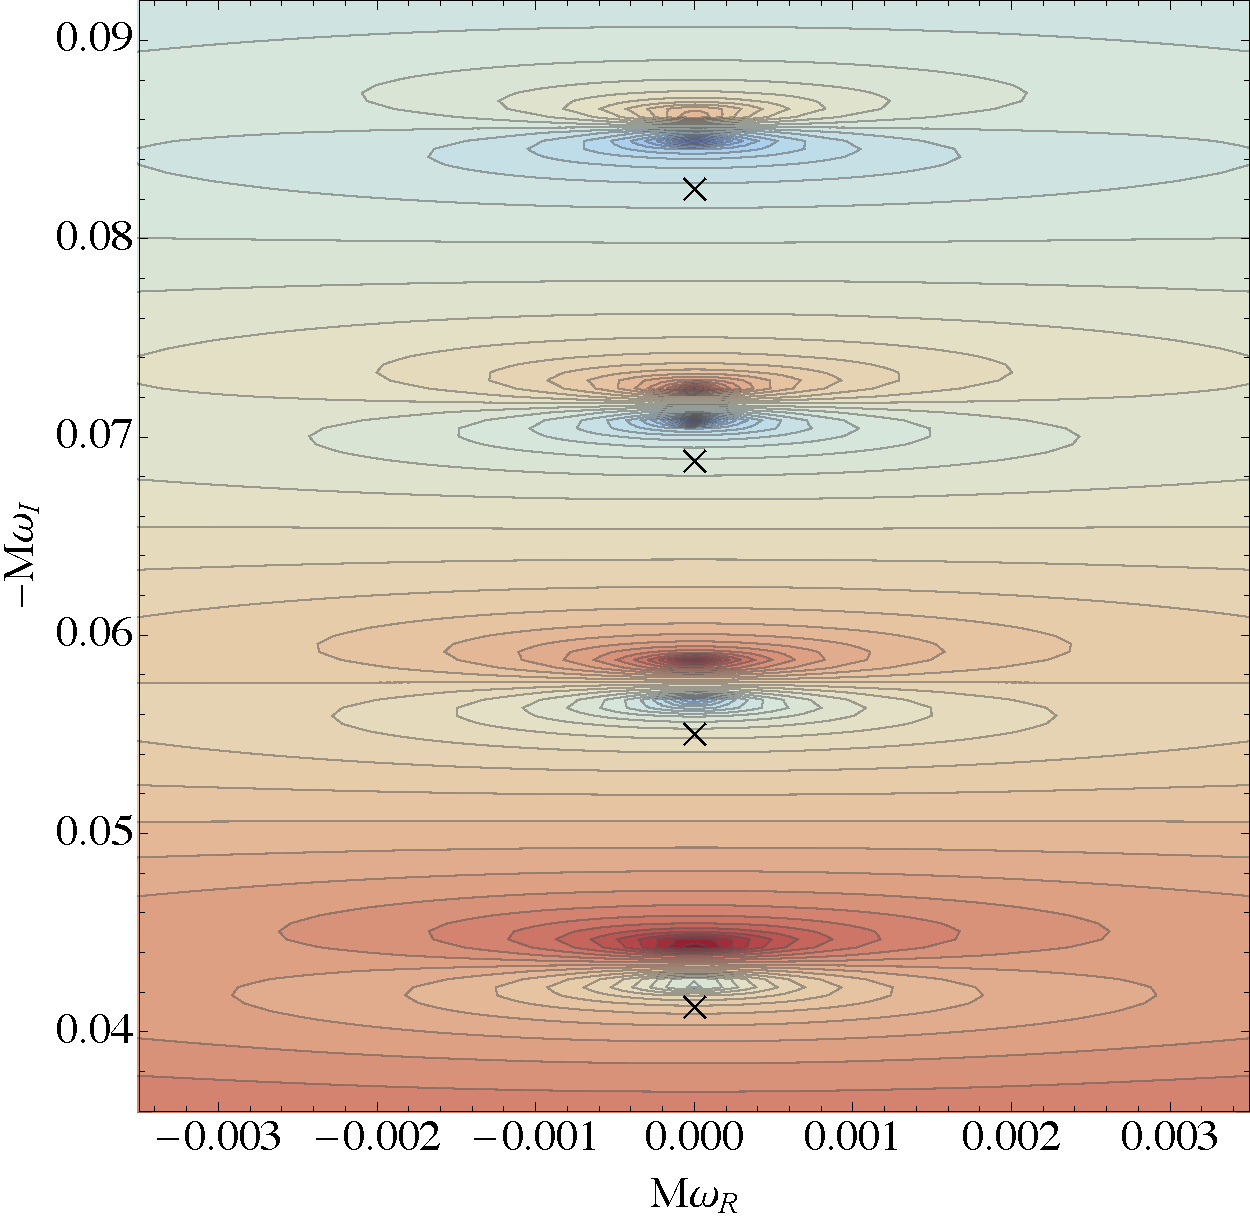
\includegraphics[width =.95 \columnwidth]{chapter_extremal/etc/RNhigh.pdf}
\caption{Contour plots of the logarithm of the magnitude of Leaver's RN continued fraction, illustrating the $l=1$ ``electromagnetic'' ZDMs (as defined in the limit $Q \to 0$) of NERN. The black crosses are the predictions of Eq.~\eqref{eq:RNfreq}. The plots focus on the four modes with the smallest decay rates. {\it Top panel}: The case $Q=0.999M$.  {\it Bottom panel}: The more extreme case $Q=0.9999M$. }
\label{fig:RNClose}
\end{figure}


While we consider the ansatz for the outer solution to be well-motivated, we must numerically check the expression for the ZDM frequencies of NERN, Eq.~\eqref{eq:RNfreq}. 
In this section, show that Eq.~\eqref{eq:RNfreq} is accurate using the methods of Sec.~\ref{sec:DFNumerics}, namely via contour plots of the logarithm of the continued fraction $\mathcal C^r$ and numerical calculations of the residual error $\Delta \omega$. 
We find that residual error in Eq.~\eqref{eq:RNfreq} scales identically to the residual error in the DF ZDM formula; $\Delta \omega \sim O[(n+1/2)\sigma^{2}]$. 
Together with the WKB results for the damped modes, this analysis demonstrates that the RN QNM spectrum also undergoes a bifurcation as $\sigma \to 0$ .

To numerically compute the QNM frequencies, we once again use Leaver's method, which can be extended with some effort to RN black holes~\cite{LeaverRN}. For RN, the angular problem decouples from the radial problem and is solved by scalar, vector, and tensor spherical harmonics with known eigenvalues.  The radial wave functions can be expanded as a power series whose coefficients obey a four-term recurrence relation. Through Gaussian elimination, these can be converted into three-term recurrence relations and then into a radial continued fraction $\mathcal C^r$ whose roots give the QNM frequencies.

In Fig.~\ref{fig:RNClose}, we present two contour plots of the logarithm of $|\mathcal C^r|$ in the complex-$\omega$ plane, for the case $j=1$ (electromagnetic-type) and $l=1$, for nearly-extremal values of charge $Q = 0.999M$ and $Q= 0.9999M$. These plots demonstrate the existence of $j=1$, $l=1$ ZDMs lying on the imaginary axis. Visually, we again see agreement with the prediction of Eq.~\eqref{eq:RNfreq} (black crosses). 

\begin{figure*}[tb]
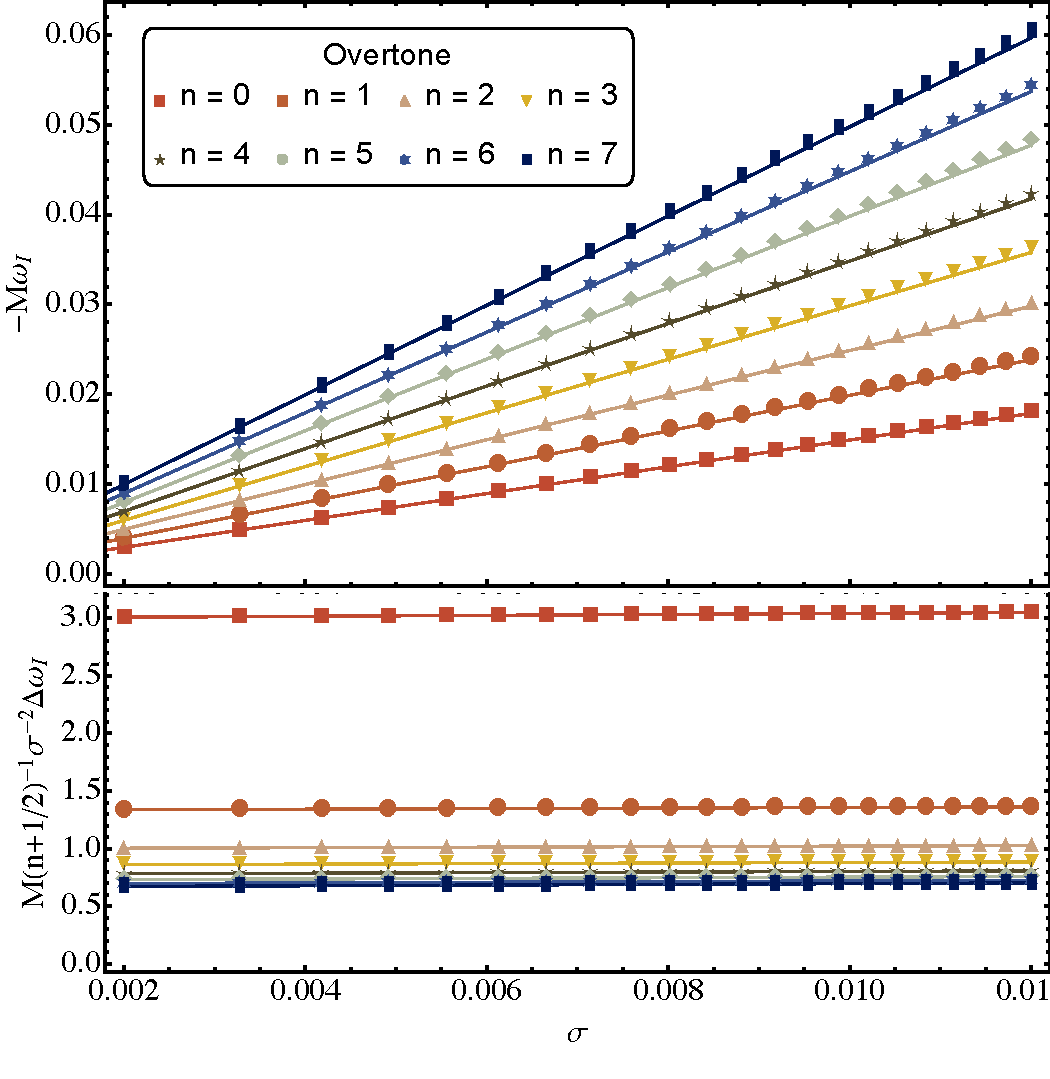
\includegraphics[width =1.0 \columnwidth]{chapter_extremal/etc/Quads1L1.pdf}
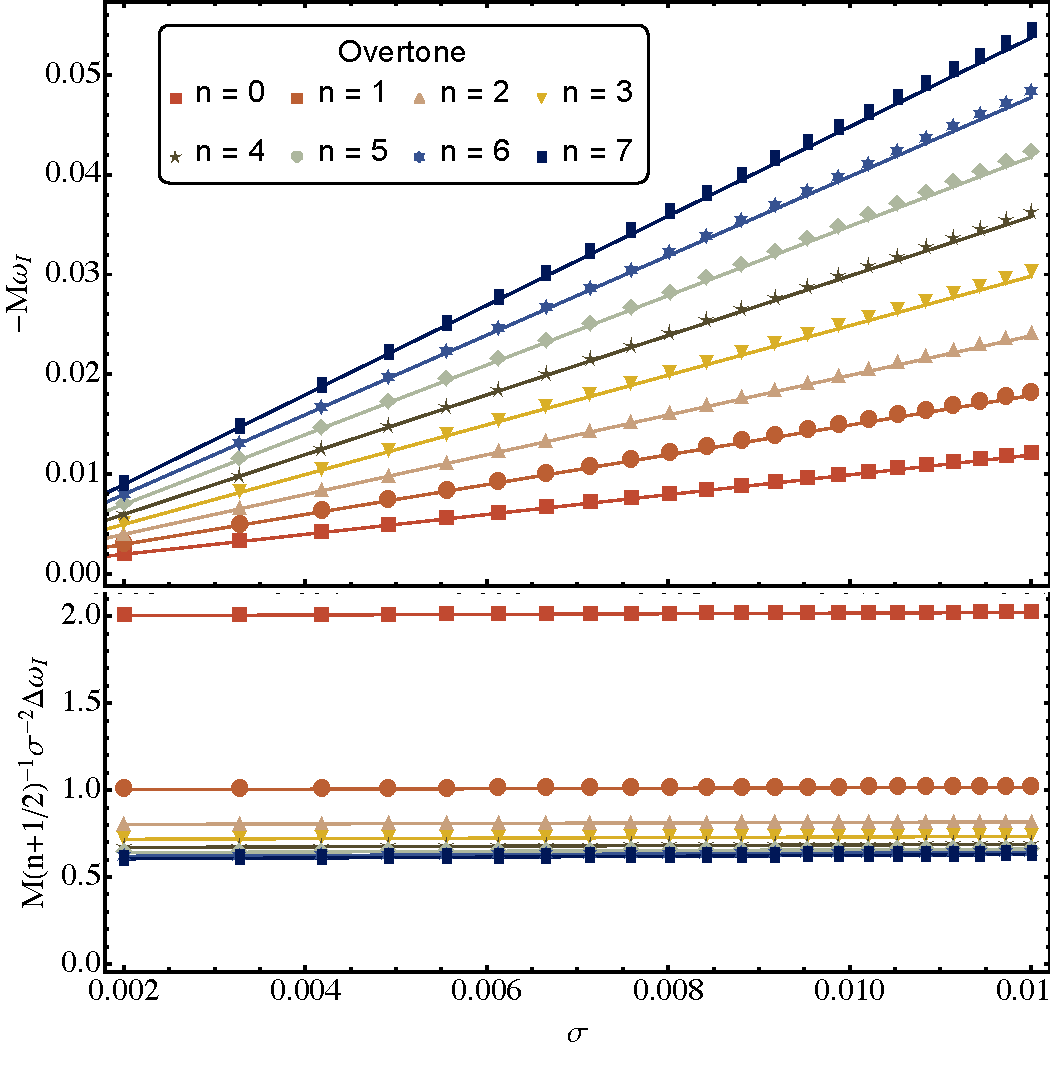
\includegraphics[width =1.0 \columnwidth]{chapter_extremal/etc/Quads2L2.pdf} \\
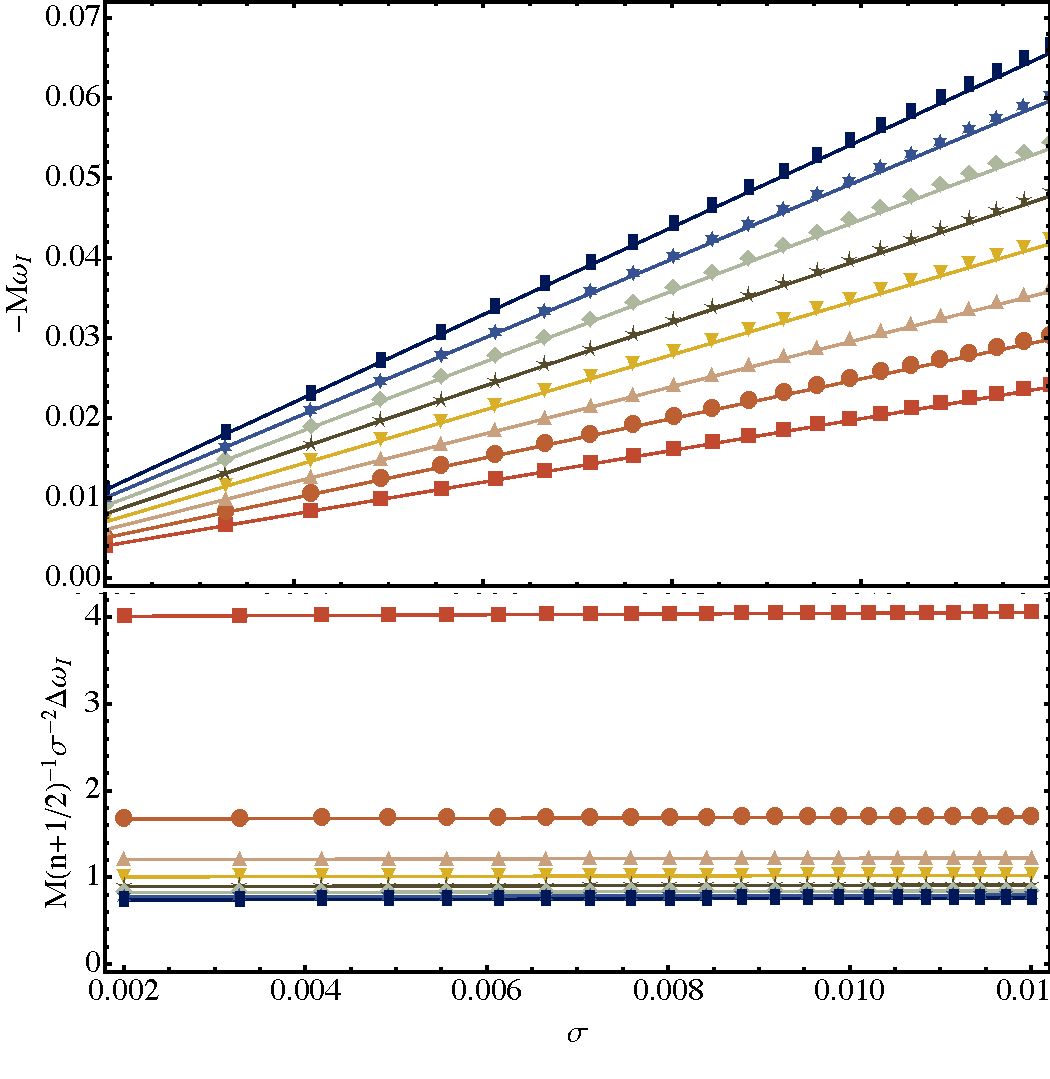
\includegraphics[width =1.0 \columnwidth]{chapter_extremal/etc/Quads1L2.pdf} 
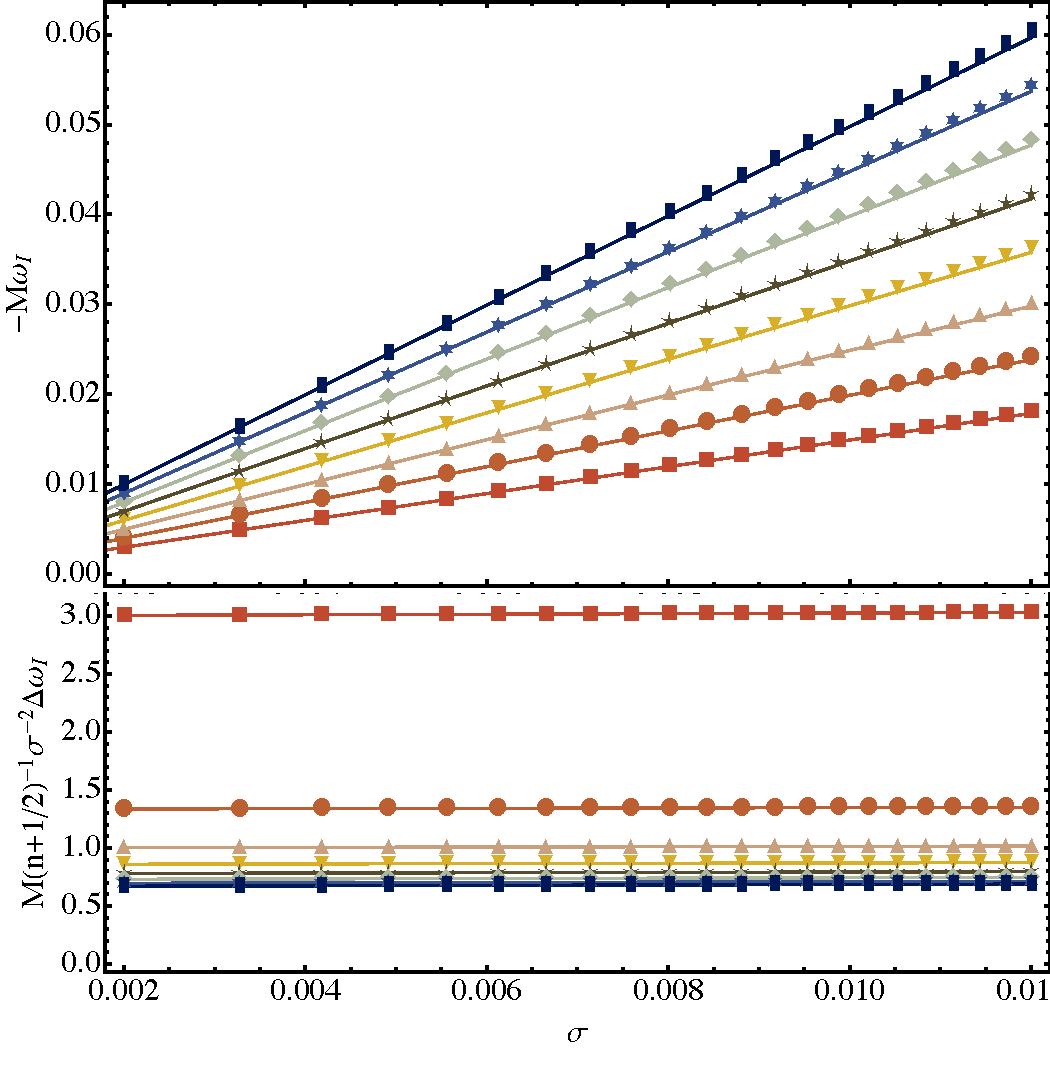
\includegraphics[width =1.0 \columnwidth]{chapter_extremal/etc/Quads2L3.pdf}
\vspace{-5mm}
\caption{ZDM frequencies for perturbations of the RN black hole. The top of each panel plots the eight lowest overtones for several values of $\sigma$, calculated with Leaver's method (points). We also plot the analytical RN ZDM frequency predictions of Eq.~\eqref{eq:RNfreq} for these overtones (lines). The bottom of each panel plots the scaled residual error of Eq.~\eqref{eq:RNfreq}, $M\sigma^{-2}(n+1/2)^{-1}\Delta \omega$ versus $\sigma$, and the lines here simply join the points. 
Following each line from right to left demonstrates that the residual is $O(\sigma^2)$ and following the calculations downward at a fixed value of $\sigma$ demonstrates that the residual is $O(n+1/2)$ at large $n$. 
{\it Top left}: The case  $j=1$, $l=1$. {\it Bottom left}: The case $j =1$, $l = 2$. {\it Top right}: The case $j = 2$, $l=2$. {\it Bottom right}: The case $j = 2$, $l=3$.}
\label{fig:slRN}
\end{figure*}

Figure~\ref{fig:slRN} presents a broader and more quantitative analysis. Each panel corresponds to a different value of $l$ and $j$ (mode type). The top of each panel plots the lowest eight overtones of the ZDMs, found using Leaver's method, along with the predictions of Eq.~\eqref{eq:RNfreq}. In the bottom of each panel, we plot the scaled residual error $M(n+1/2)^{-1}\sigma^{-2}\Delta\omega$ versus $\sigma$. For each overtone, one can check the $\sigma^2$ scaling of the residual by following the corresponding line. For each value of $\sigma$, one can check the $(n+1/2)^{-1}$ scaling by following the calculations vertically downward. 
While these results do not represent a comprehensive search for the ZDMs of RN, they give us confidence that the matching ansatz gives the correct expression for these frequencies. Importantly, our analysis establishes the existence of ZDMs of the GEM perturbations of RN black holes for the first time to our 
knowledge\footnote{During the completion of this work we became aware of the study~\cite{Couch:2012zz}, which uses methods analogous to Leaver's method on the nearly-extremal DF equation in the RN limit. That study identifies the scalar ZDMs, but incorrectly claims that the results apply to electromagnetic and gravitational perturbations.}.

\section{Conclusions}
\label{sec:Conclusions}

In this work we have given an overview of the QNMs of nearly-extremal Kerr-Newman black holes. 
While many of the results in Sec.~\ref{sec:DF} have appeared elsewhere, there are many contradictory results in the literature. We have reviewed the derivation of the ZDM frequencies for NEKN black holes, using matched asymptotic expansions. 
Using the WKB approximation for scalar fields in KN, we have discussed the existence of damped modes and given approximate formulae for these frequencies. 
Finally, using Leaver's method, we have validated these approximations, and effectively measured the higher order corrections to the nearly-extremal and WKB approximations.

By carrying out this analysis using the DF equation for spin-weighted scalars, the results of Sec.~\ref{sec:DF} can be compared to results for the true GEM modes of NEKN, in order to see how this simplistic model performs, for example by a careful comparison to numerical results. 
This is left for future studies, although we reiterate that the DF equation correctly predicts the small-charge corrections to the ZDMs of nearly-extremal Kerr black holes~\cite{Mark:2014aja}.

Since the case of scalar QNMs in NERN follows immediately from the results of Sec.~\ref{sec:DF}, in Sec.~\ref{sec:RN} we have investigated the coupled GEM equations of NERN. In this case, we have shown that ZDMs exist alongside the well known DMs, and given a frequency formulae for these modes using a matching ansatz. A numerical study using Leaver's method confirms this ansatz and again the residual errors provides higher order corrections. 
The ZDM frequency formula differs from that of the spin-weighted scalars found using the DF equation, indicating that the DF equation cannot accurately describe the ZDM frequencies for all spinning, charged black holes. 
For completeness, we have provided the WKB formulae for RN, and examined its extremal limit, concluding that the technique only describes damped modes.

While this work demonstrates the existence of a family of purely damped QNMs for RN, it is unclear what the implications of these modes are. They may assist in the shedding of black hole hair following collapse to an RN black hole, as is the case for exponentially decaying modes in Schwarzschild~\cite{Price:1971fb,Price:1972pw,wheeler1972magic}. A careful analysis of the excitation of QNMs would be required to assess the importance of these modes and their physical meaning.

Looking ahead, the daunting problem of gaining an analytic understanding of coupled GEM equations in the nearly-extremal case remains.
Two lines of evidence indicate that the GEM perturbations of NEKN admit ZDMs.
The first is the weakly-charged, rapidly rotating case discussed in Mark et al.~\cite{Mark:2014aja}.
That study computed the QNM frequencies of weakly-charged Kerr black holes in the form $\omega \approx \omega^{(0)} + Q^2 \omega^{(1)}$, where $\omega^{(0)}$ is the Kerr value. Mark et al.~showed that the DF equation provides a complete accounting of the frequency corrections $\omega^{(1)}$ to the gravitational and electromagnetic ZDMs in Kerr as the black hole angular momentum increases towards extremality.
The coefficients $\omega^{(1)}$ also begin to diverge in this limit, although they are  controlled by the smallness of $Q/Q_{\rm max}$, where $Q_{\rm max}$ is the charge of the extremal KN black hole at a given $a$.
Both of these behaviors can be explained if the full KN QNMs are ZDMs, whose frequencies are $m\Omega_H$ at leading order, with corrections proportional to the surface gravity $\kappa$.
Re-expanding such frequencies in small charge compared to $Q_{\rm max}$ recovers the apparent divergences of $\omega^{(1)}$ seen in that study, naturally suppressing them by $Q/Q_{\rm max}$.
Meanwhile the increasing accuracy of the DF equation can be understood by examining the near-horizon, near-extremal scalings of the ZDM wave functions of Kerr \cite{Mark:2014aja}, although the reason for these scalings remains a puzzle.

The other, even more compelling line of evidence is provided by the recent numerical investigations of the QNMs of KN.
The numerical results of~\cite{Dias:2015wqa} show definitively the existence of ZDMs in KN. In that study, a GEM mode with $l=m=2$ showed the behavior $\omega_R \sim m \Omega_H$ and $\omega_I \to 0$ in the extremal limit, for all values of $a$.
The fact that this occurs even when $Q \geq 0.5 M$ indicates that the search of~\cite{Dias:2015wqa} identifies the ZDMs, even in the regime where we expect DMs and where spectrum bifurcation might confuse a numerical search. 
Since~\cite{Dias:2015wqa} focused on only the lowest overtones (defined as having the smallest decay rate), future numerical studies will be required to understand the existence and behavior of the GEM damped modes of the KN black hole.

The dependence of the ZDM frequency~\eqref{eq:DFfreq} on spin and charge also explains the frequency behavior seen in the numerical simulations presented in~\cite{Zilhao:2014wqa}, as pointed out in a remark by Hod~\cite{Hod:2014uqa}. 
Those numerical simulations evolved perturbations of NEKN black holes using the full Einstein-Maxwell equations, and argued that for a range of values of $Q$ the perturbations had frequencies and decay rates dependent primarily on the combination $a/a_{\rm max} = a/ \sqrt{1 - Q^2/M^2}$. 
At first glance, this is in contradiction with our formula~\eqref{eq:DFfreq}. 
In fact the proposed relation gives almost the same frequencies as~\eqref{eq:DFfreq} for the cases $a\gtrsim0.9M, \, Q \lesssim 0.4 M$.
Only a precise analysis of the frequencies and decay rates, such as that given in \cite{Dias:2015wqa}, can differentiate the proposed relation from the one derived here.
Hod also notes that in the case presented in \cite{Zilhao:2014wqa} where $Q$ is large and the KN black hole is nearly extremal, $\Omega_H$ gives a good accounting for the observed frequency of the oscillations.

The success of the nearly-extremal approximation for describing ZDMs of scalar modes in RN and both scalar and GEM perturbations of RN begs the question of whether such methods can be applied to the full, coupled GEM perturbations of Kerr-Newman.
Unfortunately, a naive near-horizon, nearly-extremal scaling analysis indicates that these equations remain coupled in this limit, and this coupling in turn obstructs separation of the differential equations.
Nevertheless, the results of this paper, many previous studies, and recent comprehensive numerical results~\cite{Zilhao:2014wqa,Dias:2015wqa} all indicate that the ZDMs of the full coupled perturbations of NEKN obey a simple frequency formula like Eq.~\eqref{eq:DFfreq}. 
The challenge is to show that this is so, and provide an analytic expression for the factor of $\delta(a)$.
The wealth of progress in studying perturbations of KN black holes in the past several years places this goal within reach.
It may be that the connection to conformal field theories available in the near-horizon region of NEKN~\cite{Bardeen:1999px,Guica2009,Hartman:2008pb,Hartman:2009nz,Porfyriadis:2014fja} will allow for the solution of this problem, or at least to further connections to quantum theories.
Another promising avenue is the application of WKB techniques to the coupled GEM equations.
In the WKB limit, the differences between the DF and full GEM predictions for RN vanish, although the equations describe very different kinds of perturbations. 
It may be that this fact carries through to the rotating KN black hole, in which case the DF WKB predictions would give an accurate accounting of the high-frequency GEM modes of KN.
We leave the investigation of this possibility to future studies.

\section{acknowledgements}

We thank Emanuele Berti, Yanbei Chen, David Nichols, Huan Yang, An{\i}l Zengino\u{g}lu and Fan Zhang for previous collaboration and valuable discussion on the topic of the QNMs of nearly-extremal black holes. 
We are especially grateful to Huan Yang and Yanbei Chen for collaboration on additional studies of Kerr-Newman black holes and the WKB approximation for QNMs, which this study grew out of, and to Yanbei Chen and Fan Zhang for past collaboration on the implementation of Leaver's method in the Kerr spacetime. 
We also thank Sam Gralla and Alexandru Lupsasca for insights into the near-horizon region of nearly-extremal Kerr. 
AZ was supported by the Beatrice and Vincent Tremaine Postdoctoral Fellowship at the Canadian Institute for Theoretical Astrophysics during much of this work. 
ZM is supported by NSF Grant No. PHY-1404569,
CAREER Grant No. 0956189, the David and Barbara Groce Startup Fund at Caltech, and the Brinson Foundation. 
A portion of this work was carried out at the Perimeter Institute for Theoretical Physics. 
Research at Perimeter Institute is supported by the government of Canada and by the Province of Ontario though Ministry of Research and Innovation.

\section{Appendix:Details of the matching calculation}
\label{sec:MatchingApp}

In this Appendix we provide some supplementary equations related to the matching analysis of Sec.~\ref{sec:Matching}.
First we consider the outer solution, Eq.~\eqref{eq:OuterSln}.
In the limit $x \to \infty$, we use the expansion~\cite{nist}
\begin{align}
{}_1 F_1(a, b, 2 i \hat \omega x) \to \frac{\Gamma[b]}{\Gamma[a]} e^{2 i \hat \omega x}(2 i \hat \omega x)^{a-b} + \frac{\Gamma[b]}{\Gamma[b -a ]} (-2 i \hat \omega x)^{-a} \,. 
\end{align}
The first term above contributes to the part of the radial function which behaves as $R \propto e^{i \omega r_*}$ and so is an outgoing solution. Similarly, the second term contributes to the ingoing solution, which can be eliminated by a particular choice of $A$ and $B$.
The requirement that we have only outgoing waves provides the condition
\begin{align}
\label{eq:Ratio1}
\mathcal R = \frac{A}{B} & = \frac{\Gamma[-2 i \delta] \Gamma[1/2 + s + i \delta - 2 i \hat \omega]}{\Gamma[2  i \delta] \Gamma[1/2 + s - i \delta - 2 i \hat \omega]} e^{\pi \delta+ 2 i \delta \log 2 \hat \omega} \,.
\end{align}
We can also identify the outgoing and ingoing wave amplitudes in the general scattering problem. We have
\begin{align}
\label{eq:OuterAmp1}
\frac{Z^{\rm out}}{Z^{\rm hole}} & = A (2 i \hat \omega)^{-1/2 -s - i \delta + 2 i \hat \omega} \frac{\Gamma[1 + 2 i \delta]}{\Gamma[1/2 - s + i \delta + 2 i \hat \omega]} +B (\delta \to \delta) \,, \\
\label{eq:OuterAmp2}
\frac{Z^{\rm in}}{Z^{\rm hole}} & = A (-2 i \hat \omega)^{-1/2 + s - i \delta - 2 i \hat \omega} \frac{\Gamma[1 + 2 i \delta]}{\Gamma[1/2 + s + i \delta - 2 i \hat \omega]} + B (\delta \to - \delta)\,.
\end{align}
Here we have normalized each amplitude by the amplitude of the wave function at the horizon, $Z^{\rm hole}$. Elsewhere in this paper, we have assumed that $Z^{\rm hole} = 1$.

Meanwhile, in the limit of small $x$, the outer solution takes the simple form
\begin{align}
R = A x^{-1/2 - s + i \delta} + B x^{-1/2 -s - i \delta} \,.
\end{align}
The inner region provides a second condition by matching this to the inner solution. For this we transform the domain of the hypergeometric function  ${}_2 F_1$ by taking $z = 1-y$ and using the identity~\cite{nist}
\begin{align}
\label{eq:Inversion}
{}_2 F_1( \alpha, \beta, \gamma, y) & = \frac{\Gamma[\gamma] \Gamma[-2 i \delta]}{\Gamma[\gamma- \alpha]\Gamma[\gamma-\beta]} \,{}_2 F_1(\alpha, \beta, 1+ 2 i \delta, z) + \frac{\Gamma[\gamma]\Gamma[2 i \delta]}{\Gamma[\alpha]\Gamma[\beta]} z^{-2 i \delta} \,{}_2 F_1(\gamma - \alpha, \gamma -\beta, 1 -2 i \delta, z) \,.
\end{align}
It is important that in KN the parameters of the hypergeometric function obey $\gamma - \alpha - \beta = - 2 i \delta$ just as in Kerr, which allows the matching to occur. This has been used to simplify some of the terms in the above identity.
Note also that $\gamma - \alpha  = \beta|_{\delta \to -\delta}$ and $ \gamma - \beta = \alpha|_{\delta \to -\delta}$, demonstrating the symmetry of these equations under the change of the sign of $\delta$. 
This means that we can use the convention that $\delta$ is a positive real or imaginary number without loss of generality.

Next we take the limit $z \to 0$, which sets the hypergeometric functions in Eq.~\eqref{eq:Inversion} to unity.
Some useful identities for the matching are
\begin{align}
R  \approx \frac{r_+^{-s} \, x^{-s}}{\sqrt{r_+^2 +a^2}} u \,, && z \approx \frac{\sigma}{x} \,,
\end{align}
and we recall that $u = y^{-p} (1-y)^{-q} {}_2 F_1(\alpha, \beta, \gamma, y)$. 
Combining all of these equations gives us an expression for the inner solution,
\begin{align}
\label{eq:innmatch}
R & \approx \frac{r_+^{-s}}{\sqrt{r_+^2 +a^2}} x^{-s} \left(\frac{\sigma}{x} \right)^{1/2+i\delta} \left [\frac{\Gamma[\gamma] \Gamma[-2 i \delta]}{\Gamma[\gamma- \alpha]\Gamma[\gamma-\beta]} + \frac{\Gamma[\gamma]\Gamma[2 i \delta]}{\Gamma[\alpha]\Gamma[\beta]}\left( \frac{\sigma}{x}\right)^{-2 i \delta} \right] \,,
\end{align}


The matching gives 
\begin{align}
\label{eq:InnerAmp}
A & = \frac{r_+^{-s}\sigma^{1/2 - i \delta}}{\sqrt{r_+^2 + a^2}} \frac{\Gamma[\gamma] \Gamma[2 i \delta]}{\Gamma[\alpha] \Gamma[\beta]}\,, &
B & = \frac{r_+^{-s}\sigma^{1/2 + i \delta}}{\sqrt{r_+^2 + a^2}} \frac{\Gamma[\gamma] \Gamma[-2i\delta]}{\Gamma[\gamma - \alpha] \Gamma[\gamma - \beta]} \,,
\end{align}
so that 
\begin{align}
\label{eq:Ratio2}
\frac{A}{B} & = \sigma^{- 2 i \delta} \frac{\Gamma[2i\delta]}{\Gamma[-2 i \delta]}\frac{\Gamma[\gamma - \alpha]\Gamma[\gamma - \beta]}{\Gamma[\alpha]\Gamma[\beta]} \,.
\end{align}
In the general scattering problem, Eqs.~\eqref{eq:OuterAmp1}, \eqref{eq:OuterAmp2}, and \eqref{eq:InnerAmp} give the full expressions for the amplitudes, or equivalently the reflection and transmission coefficients of scalar waves in NEKN. 
The scattering amplitudes given here also allow for the calculation of QNM excitation factors, following the steps in~\cite{Yang:2013uba}. 
Since we do not deal with excitation of QNMs here, we omit these lengthy expressions.

The conditions from Eqs.~\eqref{eq:Ratio1} and~\eqref{eq:Ratio2} can be satisfied if one of the Gamma functions in~\eqref{eq:Ratio2} is near to a pole at the negative integers. 
In the case where $\delta$ is pure imaginary with our convention, Eq.~\eqref{eq:Ratio2} is suppressed by the smallness of $\sigma$, whereas Eq.~\eqref{eq:Ratio1} has no sensitive dependence on $\sigma$. 
This difference in behavior can be compensated by having one of the Gamma functions take a large value, i.e.\ be near its poles.
Meanwhile, when $\delta$ is real, then Eq.~\eqref{eq:Ratio1} exhibits rapid oscillation in phase when $\sigma$ is changed by a small amount; there is no such sensitive phase dependence on $\sigma$ in $\mathcal R$. 
The same assumption, that one of the Gamma functions is near its pole, can be used to compensate for this phase dependence, if the shift of the argument of the Gamma from its pole absorbs this rapid phase variation.
These considerations motivate the condition $\Gamma[\gamma - \beta] = \Gamma[-n - i \eta]$. Since $\gamma - \beta$ depends on the frequency through $\varpi$, this condition selects a particular QNM frequency. 
Expanding this condition in small $\eta$, we have $1/\Gamma[-n - i \eta] = (-1)^n (n!) (-i \eta) + O(\eta^2)$. We can solve the matching condition for $\eta$, giving an expression for the correction to $\omega$,
\begin{align}
\label{eq:EtaEqn}
\eta & = \mathcal R^{-1} (-1)^n \frac{i  \sigma^{- 2 i \delta}}{n!}  \frac{\Gamma[2i\delta]}{\Gamma[-2 i \delta]}\frac{\Gamma[\gamma - \alpha]}{\Gamma[\alpha]\Gamma[\beta]}\,.
\end{align}
As discussed in~\cite{Yang:2013uba}, $\eta$ is generally quite small, with the exception of cases where $\delta^2$ is small and negative, in which case it can be order unity or greater. 
Although the possibility has not been explored in detail, there may even be situations where $\eta$ could be large enough to invalidate the approximation used above to find a closed form solution for the ZDM frequencies.
We do not incorporate the correction $\eta$ into our frequency formula in this work, but in cases where $\eta$ is a significant contribution to the $O(\sigma)$ frequency corrections, Eq.~\eqref{eq:EtaEqn} can be used to augment the ZDM frequency formula. 
In addition, whenever $\eta \gtrsim \sigma$, it dominates the residual error in our frequency formula. 
In Sec.~\ref{sec:DFNumerics} for $l=m=2$, $s=1$ and $\delta^2>0$, we find that the term $\sigma \eta$ prevents $O(\sigma^2)$ scaling of the residual errors at small values of $\sigma$.

\section{Appendix: The WKB analysis of the Dudley-Finley equations}
\label{sec:WKBApp}

\begin{figure*}[t]
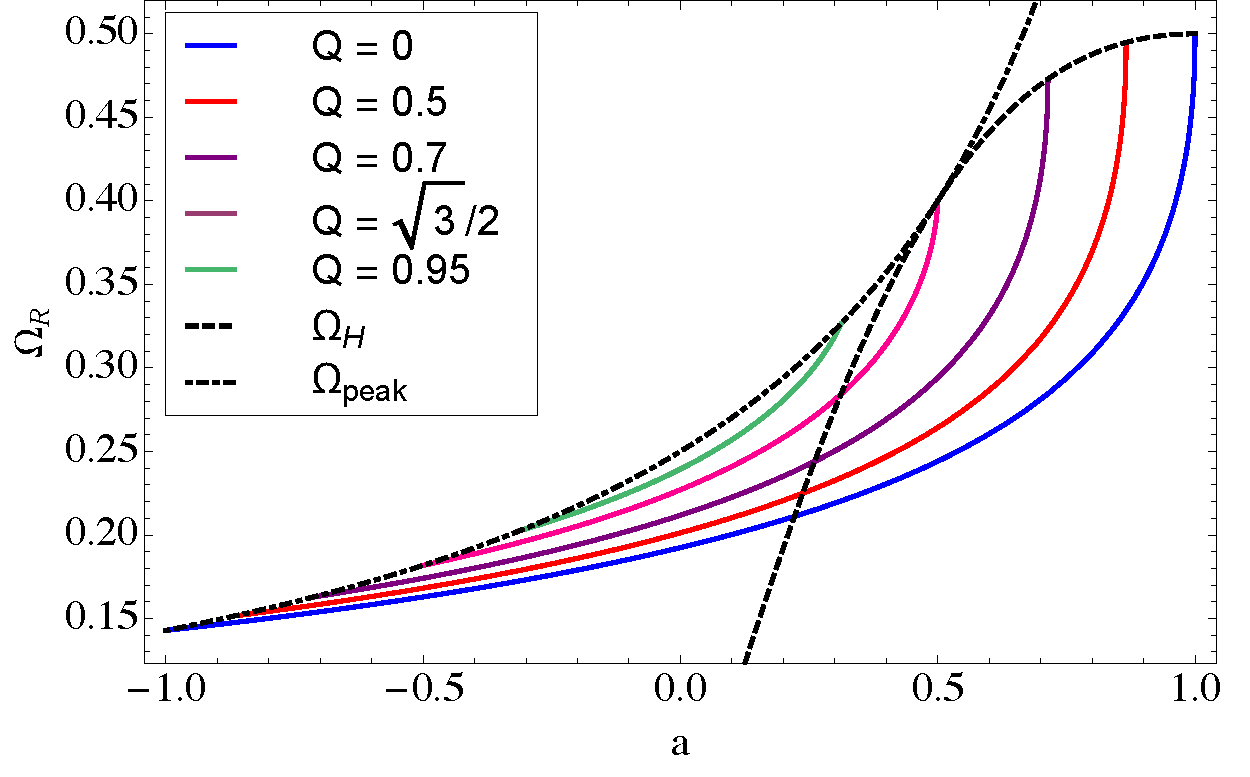
\includegraphics[width = 0.48 \columnwidth]{chapter_extremal/etc/WKBFreqFixQ}
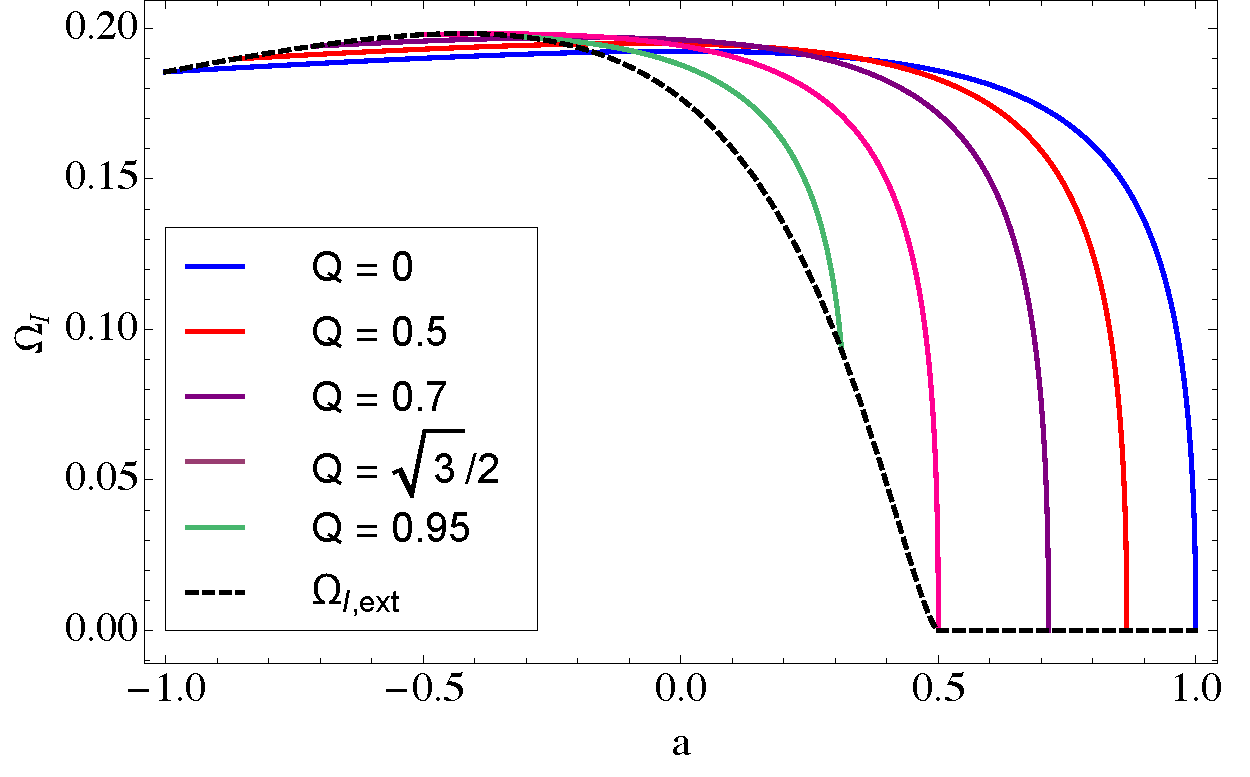
\includegraphics[width = 0.48 \columnwidth]{chapter_extremal/etc/WKBDecayFixQ}
\caption{{\it Left panel}: The scaled WKB frequency $\Omega_R$ as $a$ varies for fixed values of $Q$, in the case $\mu = 1$. From the far right to left the curves are for $Q=0$ to $Q = 0.95$. Also plotted are the two extremal limits, $\Omega_H$ and $\Omega_{\rm peak}$ [Eq.~\eqref{eq:WKBFreqOuterPeak}].
{\it Right panel}: The scaled WKB decay rate $\Omega_I$ as $a$ varies for the same cases as the top panel. From far right left the curves again are for $Q = 0$ to  
$Q = 0.95$. Also plotted is the extremal prediction $\Omega_{I, {\rm ext}}$ [$0$ for $\mu>\mu_c$ and otherwise given by Eq.~\eqref{eq:DMExDecay}].
}
\label{fig:WKBFreqFixQ}
\end{figure*}

The WKB analysis of the Dudley-Finley equation in the Kerr-Newman spacetime is a straightforward extension of the methods discussed in~\cite{Schutz:1985zz,IyerWill1987} and later extended for generic orbits in Kerr~\cite{Yang:2012he}. 
The result of this analysis gives Eqs.~\eqref{eq:WKBSolve} and~\eqref{eq:WKBOmegaI} for the WKB frequency and decay rates, using the leading order parts of the radial potential for the DF equation.
We present the relevant equations here in full, and specialize to the near-extremal case in Sec.~\ref{sec:WKBanalysis}. For convenience in this section we set $M=1$.
Solving both of Eqs.~\eqref{eq:WKBSolve} while eliminating $\lambda$ gives our useable formula for $\Omega_R$,
\begin{align}
\label{eq:WKBOmegaR}
\Omega_R & = \frac{\mu a (r - 1)}{(r^2 +a^2)(r -1) - 2 r \Delta}\,,
\end{align}
which must be evaluated at the peak $r_0$ to give a consistent solution to the WKB equations. The above is only an implicit equation for $\Omega_R$ unless we can determine $r_0$ independently of $\Omega_R$. 
Equation~\eqref{eq:WKBOmegaR} shows that if $r_0$ approaches the horizon, $\Omega_R$ approaches the horizon frequency $\Omega_H$. 
This is in agreement with the situation in Kerr, and is only modified by the fact that $\Omega_H$ depends on both $a$ and $Q$.

Using both conditions of Eqs.~\eqref{eq:WKBSolve} together with the approximate analytic expression \eqref{eq:AppxA} for $\alpha(\mu,a,Q)$, lets us eliminate $\Omega_R$, yielding a sixth order polynomial equation, 
\begin{align}
\label{eq:WKBPoly}
2 r^2[r(r-3)+2Q^2]^2 + 4 r\left(r[r^2(1-\mu^2) - 2r -3 (1-\mu^2)]+2Q^2(1-\mu^2 +r) \right)a^2
\notag \\ 
+(1-\mu^2)[r^2(2-\mu^2) + 2r(2+\mu^2) + 2-\mu^2]a^4 =0 \,.
\end{align}
The outermost root of this polynomial gives the position of the peak $r_0$, and when Eq.~\eqref{eq:WKBOmegaR} is evaluated at $r_0$ we attain a self-consistent solution to the equations. 
Note that in the $a \to 0$ case, both the numerator and denominator of Eq.~\eqref{eq:WKBOmegaR} vanish. A better behaved expression in this limit can be found by using the polynomial~\eqref{eq:WKBPoly} to eliminate the vanishing denominator; after some simplification we find
\begin{align}
\label{eq:WKBOmegaRSecond}
\Omega_R = \frac{\sqrt{2}(r - M)}{\sqrt{4r(r^3 - 3 r +2 Q^2) + a^2[(r^2+M)(3-\mu^2)+2r(1+\mu^2)]}}\,.
\end{align}
This equation also behaves correctly in the case $\mu = 0$, for which additional, closed form analytic expressions can be derived for $r_0$ and the frequencies (see e.g~\cite{Teo2003,Dolan2010,Yang:2012he} for the Kerr case). Meanwhile, it is poorly behaved when $r_0$ approaches the horizon in the extremal case, and so is not used outside of this Appendix. 

The WKB analysis gives an equation for $\Omega_I = \omega_I/(n+1/2)$, Eq.~\eqref{eq:WKBOmegaI}.
Using some algebraic tricks that rely on the conditions in Eq.~\eqref{eq:WKBSolve}, we get
\begin{align}
\Omega_I = \left. \Delta\frac{\sqrt{ 4(6 \Omega_R^2 r^2 -1) + 2 a^2 \Omega_R^2(3-\mu^2) }}{2 \Omega_R(r^2+a^2)^2 - 2\mu a (r^2 +a^2) -a \Delta [a \Omega_R (1+\mu^2) - 2 \mu] } \right|_{r_0} \,.
\end{align}
We see immediately that if $r_0$ goes to the horizon in the extremal limit, the WKB analysis predicts a vanishing $\omega_I$, which indicates the existence of ZDMs. 

In Fig.~\ref{fig:WKBFreqFixQ} we plot some representative values of $\Omega_R$ and $\Omega_I$ at fixed charge $Q$ and maximum inclination parameter $\mu = 1$, for values of $a$ varying between each extremal case. For positive values of $a$, the WKB modes correspond to corotating equatorial photon orbits, while for negative values of $a$ they correspond to counter-rotating equatorial orbits.


\printbibliography[heading=subbibliography]
\end{refsection}
%\begin{refsection}

\newcommand{\ba}{\begin{align}}
\newcommand{\ea}{\end{align}}
\newcommand{\p}{\partial}
\newcommand{\lm}{_{\ell m}}
\newcommand{\bma}{\begin{pmatrix}}
\newcommand{\ema}{\end{pmatrix}}
\newcommand{\R}[1]{\textcolor{red}{#1}}
\newcommand{\aaron}[1]{\textcolor{Orange}{#1}}
\newcommand{\zach}[1]{\textcolor{ForestGreen}{#1}}
\newcommand{\ac}[1]{\textcolor{cyan}{\sout{#1}}}


\newcommand{\Rb}{\tilde{\mathcal R}}
\newcommand{\TBH}{\tilde{\mathcal T}_{\rm BH}}
\newcommand{\RBH}{\tilde{\mathcal R}_{\rm BH}}
\newcommand{\K}{\tilde{\mathcal K}}
\newcommand{\RW}{\tilde{\mathcal R}_{\rm W}}

\newcommand{\psiupA}{\tilde \psi_{\rm up}}%For some reason I'm getting errors when I try to name the command \psiup as in the paper so I'm calling it \psiupA
\newcommand{\psiin}{\tilde \psi_{\rm in}}
\newcommand{\psiref}{\tilde \psi_{\rm ref}}
\newcommand{\psiecho}{\tilde \psi_{\rm echo}}
\newcommand{\gref}{\tilde g_{\rm ref}}
\newcommand{\gBH}{\tilde g_{\rm BH}}
\newcommand{\ZinfBH}{Z^{\infty}_{\rm BH}}
\newcommand{\ZhBH}{Z^{\rm H}_{\rm BH}}
\newcommand{\Zref}{Z^{\infty}_{\rm ref}}
\newcommand{\Zecho}{Z_{\rm echo}}

\chapter{A recipe for echoes from exotic compact objects}
\label{chap:Echo}

\begin{centering}
Zachary Mark, Aaron Zimmerman, Song Ming Du, and Yanbei Chen \\
Phys. Rev. D 96, 084002 (2017) \\
\href{https://https://arxiv.org/abs/1706.06155}{arxiv:1706.06155} \\
\end{centering}

\section{Abstract}
Gravitational wave astronomy provides an unprecedented opportunity to test the nature of black holes and search for exotic, compact alternatives. 
Recent studies have shown that exotic compact objects (ECOs) can ring down in a manner similar to black holes, but can also produce a sequence of distinct pulses resembling the initial ringdown. 
These ``echoes'' would provide definite evidence for the existence of ECOs. 
In this work we study the generation of these echoes in a generic, parametrized model for the ECO, using Green's functions.
We show how to reprocess radiation in the near-horizon region of a Schwarzschild black hole into the asymptotic radiation from the corresponding source in an ECO spacetime.
Our methods allow us to understand the connection between distinct echoes and ringing at the resonant frequencies of the compact object.
We find that the quasinormal mode ringing in the black hole spacetime plays a central role in determining the shape of the first few echoes. 
We use this observation to develop a simple template for echo waveforms.
This template preforms well over a variety of ECO parameters, and with improvements may prove useful in the analysis of gravitational waves.

\section{Introduction}

The existence of event horizons is one of the most astonishing predictions of General Relativity.  
Horizons generically \cite{Thorne:1972ji} form during the gravitational collapse of classical matter and are expected to be common occurrences in our universe. 
Observations of black holes are undergoing a revolution, with the advent of gravitational wave astronomy \cite{Abbott:2016blz,Abbott:2016nmj,TheLIGOScientific:2016pea,LIGO:GW170104} and the promise of very-long-baseline radio observations of supermassive black holes by the Event Horizon Telescope \cite{Falcke:1999pj,Johnson:2015iwg}.
While black holes are consistent with all electromagnetic and gravitational wave observations to date \cite{TheLIGOScientific:2016src,Yagi:2016jml,Yunes:2016jcc,TheLIGOScientific:2016pea,LIGO:GW170104}, no experiment has been able probe spacetime near the event horizon \cite{Eckart:2017bhq,Abramowicz:2002vt,CardosoReview}.
Moreover, the event horizon is at  the heart of the BH information paradox \cite{Unruh:2017uaw}, and the role of black holes in a quantum theory of gravity is an open question. 

These puzzles have inspired proposals for horizonless alternatives to black holes including gravastars \cite{Mazur:2001fv}, boson stars \cite{Schunck:2003kk}, wormholes \cite{Morris:1988tu}, fuzzballs \cite{Mathur:2005zp} and others \cite{Barcelo:2010vc, Barcelo:2014cla,Holdom:2016nek}. 
Many of these exotic compact objects (ECOs) can be ruled out on theoretical grounds.
ECOs with angular momentum often suffer from a superradiant instability, although this instability can quenched by tuning the compactness and other parameters describing the ECO \cite{Maggio:2017ivp,Hod:2017cga}. Cardoso et al.~\cite{Cardoso:2014sna} have conjectured that any ECO with an unstable photon orbit may suffer from nonlinear instabilities.

While the gravitational wave astronomy has the potential to probe black holes (BHs) like never before \cite{Yagi:2016jml}, distinguishing BHs from highly compact ECOs will be difficult. 
The problem is that astrophysical processes are usually insensitive to the spacetime geometry near the horizon, and highly compact ECOs behave very similarly to BHs \cite{Abramowicz:2002vt}.
Attempts to distinguish merging BHs from merging ECOs using inspiral waveforms are plagued by the strong equivalence principal, which means that  the properties of extended self-gravitating bodies only appear in the  equations of motion at high post-Newtonian order. 
Nonetheless, several promising studies \cite{Porto:2016zng,Cardoso:2017cfl,Maselli:2017cmm} predict tidal distortion and tidal heating effects will allow LISA \cite{AmaroSeoane:2012km} to distinguish merging black holes from highly compact, merging ECOs (see also e.g.~\cite{Pani:2010em,Krishnendu:2017shb} for tests incorporating inspirals). 

Spacetime near the event horizon has an especially interesting effect on the ringdown waveform of the merging objects. 
Standard tests of the nature of the final merged object call for the black hole's resonant frequencies \cite{Nollert, Berti2009, Kokkotas:1999bd}, known as quasinormal mode (QNM) frequencies, to be extracted from the ringdown portion of the waveform and compared to theoretical calculations \cite{Dreyer2004,Berti:2005ys,Pani:2013pma,Berti:2016lat,Yang:2017zxs,Maselli:2017kvl}. Working in the test particle limit, Cardoso et al.~\cite{Cardoso:2016rao} pointed out that in the case of highly compact wormholes, the ringdown of the final ECO is initially nearly identical to that of a BH  despite the fact that QNM spectrum is radically changed \cite{Ching:1995rt, Nollert:1998ys,Pani:2009ss}. 
A naive application of the QNM based tests would be fooled by a highly compact ECO.   

However, Cardoso et al.~\cite{Cardoso:2016rao} also realized that the later portion of the ringdown of highly compact ECOs contains a train of decaying echo pulses (note that similar observations have been made before; see for example  \cite{Kokkotas:1995av,PhysRevD.60.024004,Ferrari:2000sr}). 
The time delay between the echoes is related to the ECO compactness while the decay and shape of each pulse encodes the reflective properties of the ECO. 

Further work established that this picture was robust \cite{Barcelo:2017lnx} across many different ECO models with many different test particle sources, but breaks down for less compact ECOs, which sometimes have ringdowns consistent with the resonant frequencies of the ECO \cite{Cardoso:2016oxy,Price:2017cjr}.
Price and Khanna conjectured that the echoes can be considered as a superposition of the resonant modes of the ECO \cite{Price:2017cjr}. 
V\"{o}lkel and Kokkotas \cite{Volkel:2017kfj} then provided a method for inferring the exact details of the ECO model from the ECO modes. 
Namely, they demonstrated that the effective scattering potential experienced by the gravitational waves could be approximately reconstructed with a knowledge of ECO spectrum.

Recently, it has been proposed that LIGO has observed echoes in the binary black hole waveforms \cite{Abedi:2016hgu, Abedi:2017isz}. While there has been much skepticism in the community \cite{Ashton:2016xff}, such tests will only become more definitive as LIGO accumulates binary merger observations. 

Most of the past studies have been in the context of a particular ECO model, using specific orbits for the merging objects.
The goal of this work is explicitly relate waveforms from  black holes to waveforms from  ECOs.
We study evolution of test scalar fields as a proxy for gravitational perturbations, which allows us to replace a generic ECO with simple reflecting boundary conditions in a BH spacetime.
We use this formalism to show that the ECO waveform can be understood either as a superposition of echo pulses or as a superposition of ECO modes and illustrate the types of behavior that can arise. 
We investigate which features of the BH waveforms shape the first few echoes, leading to a simple template for the ECO waveform.

In Sec.~\ref{sec:wavebc} we review the basic equations obeyed by the scalar field. 
We parameterize (completely) the influence of the ECO on scalar waves in the exterior vacuum region by a complex frequency-dependent reflectivity (a slight generalization of the models used in \cite{Maggio:2017ivp,Hod:2017cga,Nakano:2017fvh}). 
In Sec.~\ref{sec:ECOvsBH} we relate the ECO and BH waveform by determining the relationship between the ECO and BH Green's function. 
We find that the ECO waveform can be constructed from the BH waveform and a reprocessed version of the waveform observed on the BH horizon.
In Sec.~\ref{sec:Echoes} we show how the extra piece of the ECO waveform can be expressed as sum of echoes.
In Sec.~\ref{sec:ECOModes} we discuss the relationship between the ECO QNMs and the BH QNMs and study the ECO mode spectrum numerically for two particular ECO models. In Sec.~\ref{sec:SingleMode} and Sec.~\ref{sec:EchoInt}, we show how the difference between the ECO waveform and the BH waveform can be expressed as a superposition of ECO modes. 
In Sec.~\ref{sec:Gen} we determine general properties of the individual echoes and develop a simple template for the ECO waveform.
We also study the energy in the ECO waveform, discovering a simple relationship to the energy in the black hole waveforms reaching infinity and passing through the horizon. 

During the final stages of this work, we learned of the work of Nakano et al.~\cite{Nakano:2017fvh}, who discussed gravitational perturbations in the Kerr spacetime and arrived at a similar expression for ECO waveforms by different means.

\section{Waves near a compact object}

\subsection{Wave Equation and Boundary Conditions}
\label{sec:wavebc}

We focus on static, spherically symmetric exotic compact objects.
In this setting, an ECO consists of an exterior Schwarzschild spacetime patched to a spherically symmetric interior metric at an areal radius $r=r_0$.

We study a massless scalar field $\Phi(x^\mu)$ that obeys the sourced, curved spacetime wave equation,
\begin{align}
\Box \Phi = - \rho \,.
\end{align}
If we define the scalar $\psi (x^\mu) = r \Phi$ and decompose this scalar into frequency and spherical harmonics \cite{Casals:2015oaa},
\begin{align}
\psi (x^\mu) &= \int_{-\infty}^{\infty} \frac{d\omega}{2\pi}\sum_{\ell, m} \tilde \psi_{\ell m}(\omega,r) Y_{\ell m}(\theta, \phi)e^{-i\omega t} \,, \\
\rho (x^\mu) &= \int_{-\infty}^{\infty} \frac{d\omega}{2\pi}\sum_{\ell, m} \tilde \rho_{\ell m}(\omega,r) Y_{\ell m}(\theta, \phi)e^{-i\omega t} \,,  
\end{align}
then the wavefunctions $\tilde \psi_{\ell m}$ obey the following radial equation, 
\begin{align}
\label{eq:RW}
\frac{d^2 \tilde \psi\lm}{dx^2} &+\left(\omega^2-f V \right) \tilde \psi\lm= \tilde S \,, \\
\tilde S(\omega,x) & \equiv - r(x) f \rho\lm(\omega,x) \,.
\end{align}
Here $x$ is the usual tortoise coordinate, defined through
\begin{align}
\frac{dx}{dr} & = \frac{1}{f(r)} \,,
\end{align}
while the metric component $f(r)$ and the potential $V(r)$ depend on the particular spacetime.
In the exterior, Schwarzschild portion of the spacetime,
\begin{align}
f & = 1 - \frac{2M}{r} \,, & V & = \frac{\ell(\ell +1)}{r^2} + \frac{2M}{r^3}\,, 
\end{align}
and we treat $f$ and $V$ as implicit functions of $x$ through $r(x)$, with 
\begin{align}
x = r + 2M\ln\left(\frac{r-2M}{M}\right)\,.
\end{align}
From here we suppress the harmonic indices $(\ell,m)$.

The scalar field $\tilde \psi$ obeys an outgoing wave boundary condition $\tilde \psi \sim e^{i\omega x}$ as $x\to \infty$. 
In addition, it obeys a boundary condition inside the ECO, such as regularity at $r=0$. 
For wormholes, one would instead insist that the waves were outgoing at null infinity on the other side of the throat.

When the ECO is very compact, $r_0/(2M)-1 \ll 1$, and all sources are restricted to reside in the Schwarzschild portion of the spacetime, we may replace the second boundary condition with a reflecting boundary condition at the ECO surface $r_0$. Namely, near the ECO the potential is small, $V\approx 0$, and $\tilde \psi$ is a linear combination of ingoing and outgoing waves $e^{\pm i\omega x}$. Therefore near the ECO surface $x_0 = x(r_0)$, we must have
\begin{align}
\label{eq:refBC}
\tilde \psi \propto e^{-i\omega (x-x_0)}+\Rb(\omega) e^{i\omega (x-x_0)} \,.
\end{align}
for some frequency dependent reflectivity $\Rb(\omega)$. If $|\Rb(\omega)|=1$, the scalar field is completely reflected by the ECO.

With this insight, we can study wave emission and propagation in the ECO spacetime using a Schwarzschild BH equipped with a reflecting boundary, as shown in Fig.~\ref{fig:BCs}.
This perspective is useful since it allows us to reprocess the emission by test particles in a BH spacetime into the corresponding emission in the ECO spacetime, by taking the reflecting boundary into account. From here on we can focus on BH spacetimes, and compare wave propagation with the usual boundary conditions at the horizon to the case of a reflecting boundary. 

\begin{figure}[t]
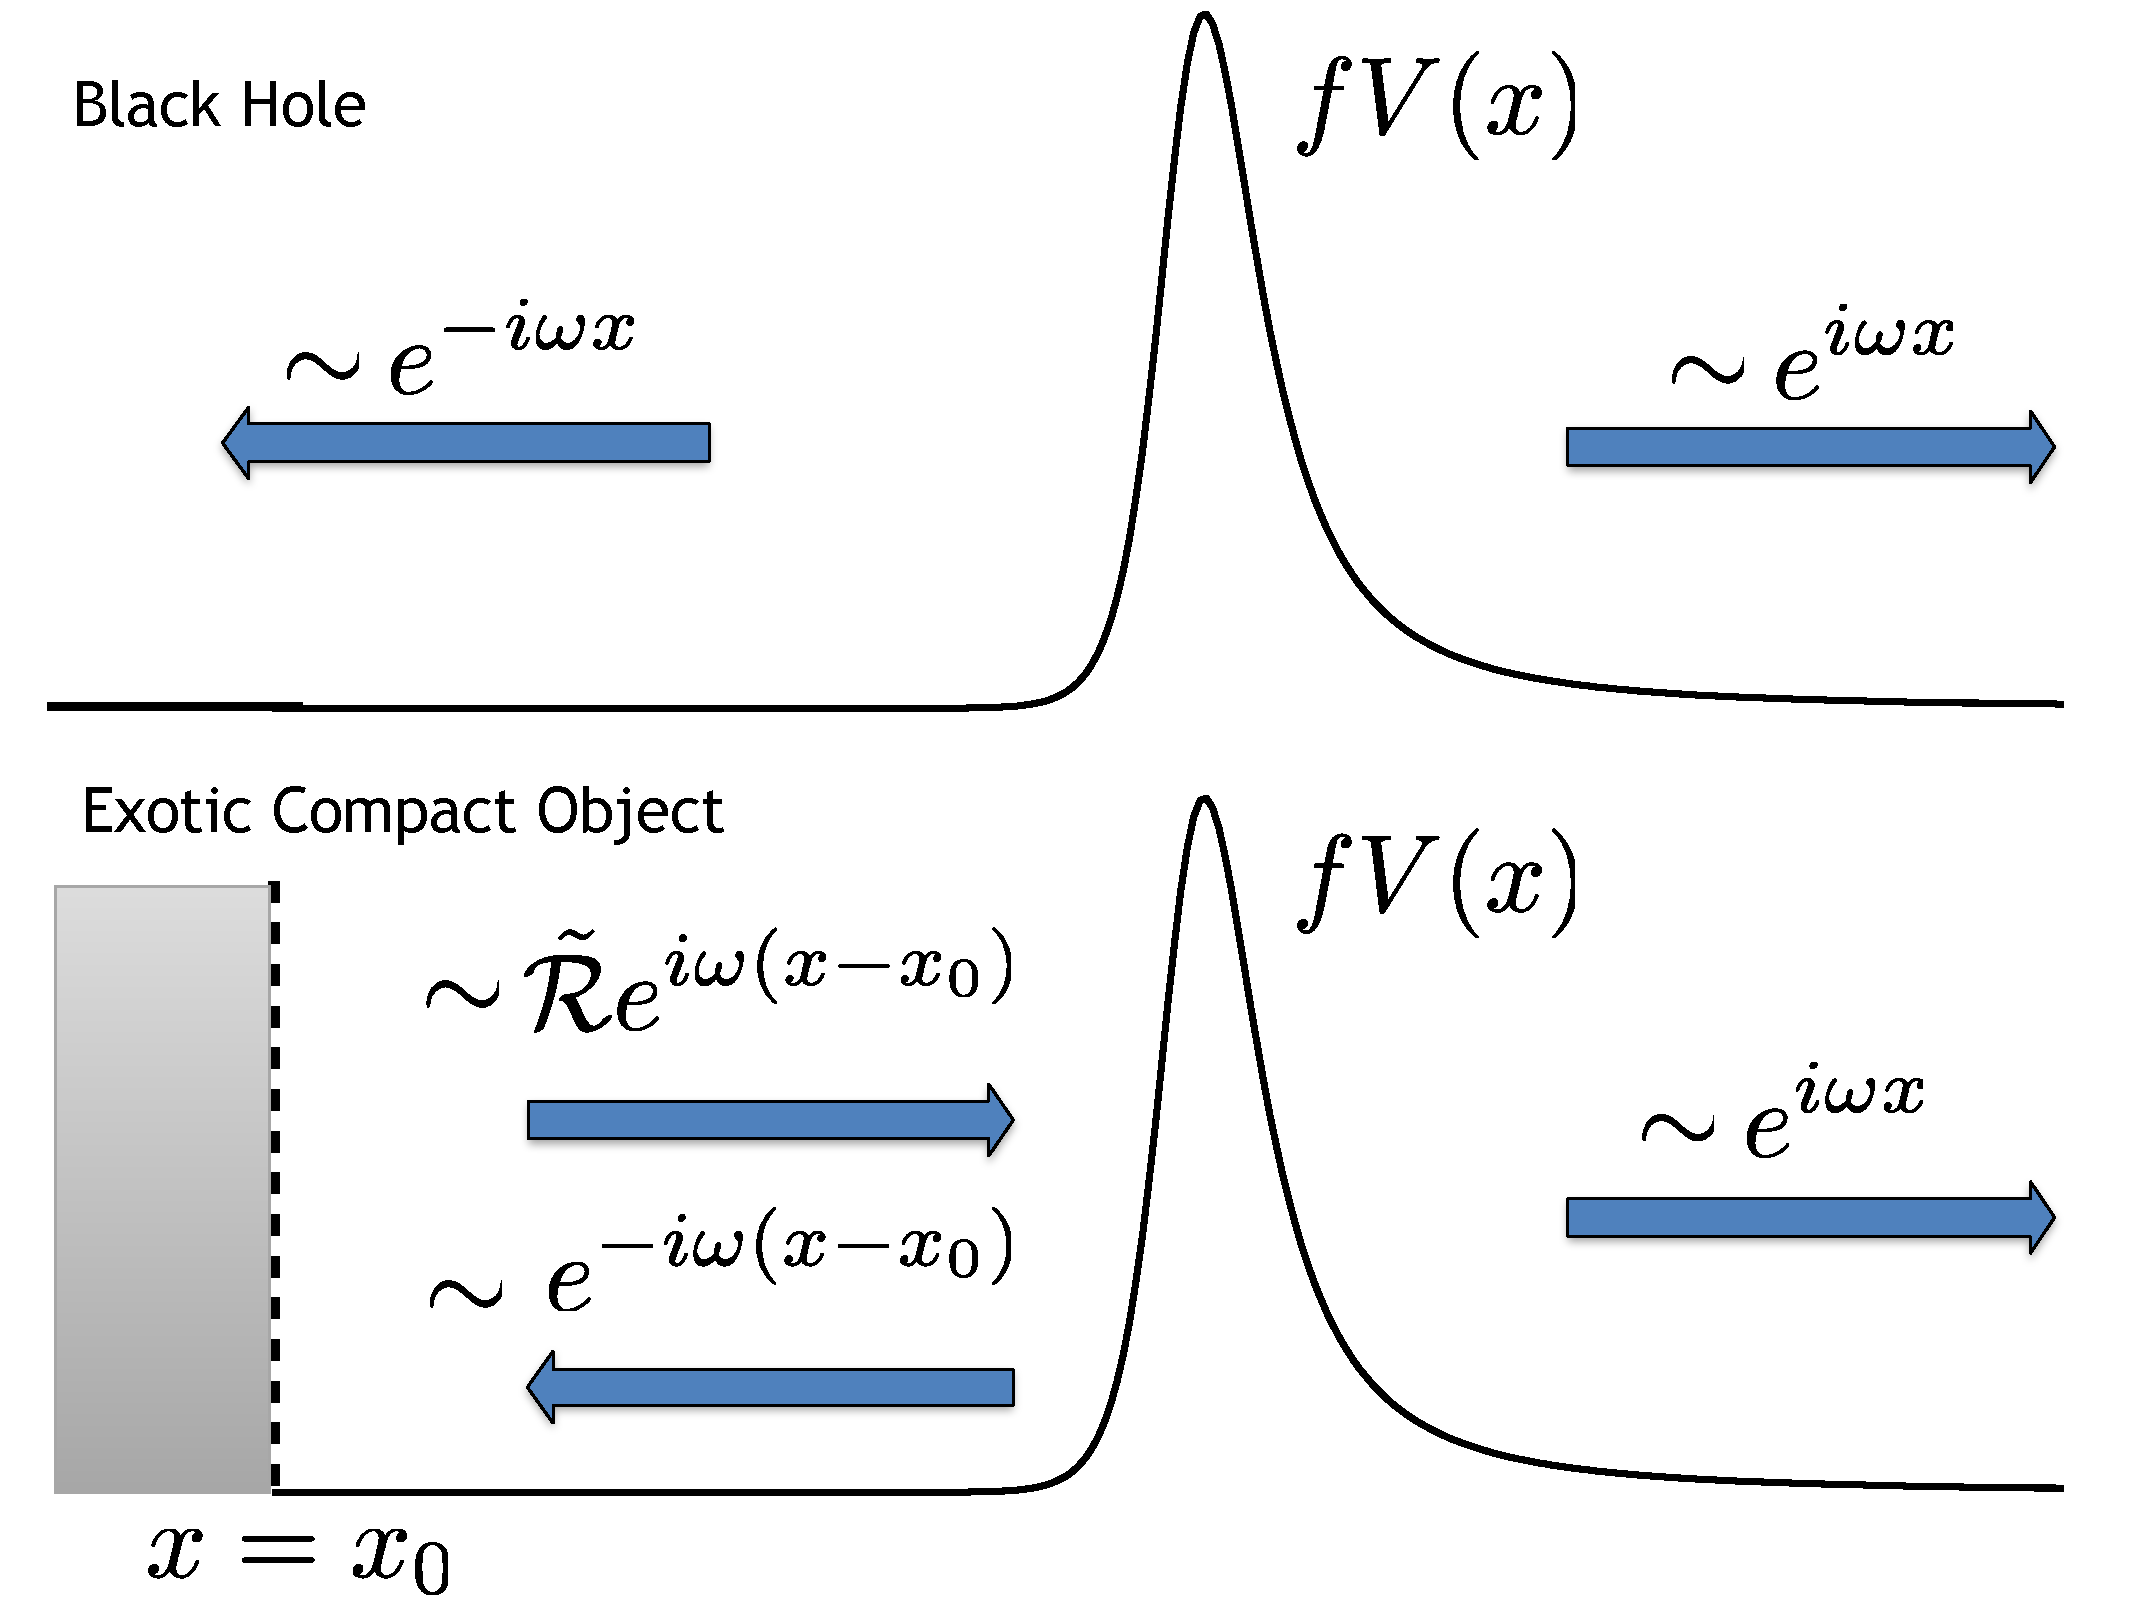
\includegraphics[width =0.98 \columnwidth]{chapter_echo/etc/BCfig}
\caption{Top: The boundary conditions for waves propagating on a black hole spacetime. Bottom: The reflecting boundary conditions for the waves in the exterior of an ECO.
}
\label{fig:BCs}
\end{figure}

\subsection{Generating ECO waveforms from BH waveforms}

\label{sec:ECOvsBH}

We are interested in computing the scalar waves seen by distant observers in a BH spacetime with a reflecting boundary.
For this we wish to construct the scalar radial Green's function $\gref(x,x')$, which obeys the scalar wave equation with a delta function source,
\begin{align}
\label{eq:RWGF}
\frac{d^2 \gref}{dx^2} + \left( \omega^2 - f V \right) \gref = \delta(x-x') \,,
\end{align}
and the reflecting boundary condition \eqref{eq:refBC}.
With the Green's function, we can compute the field produced by sources $\tilde S$ through integration,
\begin{align}
\label{eq:Sourcedpsi}
\tilde \psi(x) & = \int_{-\infty}^{\infty} dx' \, \gref(x,x') \tilde S(x')\,.
\end{align}
We compute $\gref$ for sources outside the reflecting boundary, $x'>x_0$.

To compute $\gref$ we first recall how the scattering of waves works in the usual Schwarzschild spacetime \cite{Frolov:1998wf}.
Consider the two linearly independent, homogeneous solutions $\psiin$,
\begin{align}
\psiin & \sim 
\left \{
\begin{array}{ll}
A_{\rm out}(\omega) e^{i \omega x} + A_{\rm in}(\omega) e^{-i\omega x}\,, & x \to \infty \,, \\
e^{-i\omega x}\,, & x \to - \infty \,, \\
\end{array} \right. \label{eq:psiin}
\end{align}
which is purely outgoing at the horizon, and $\psiupA$,
\begin{align}
\psiupA & \sim 
\left \{
\begin{array}{ll}
e^{i\omega x} \,, & x \to \infty \,, \\
B_{\rm out}(\omega) e^{i \omega x} + B_{\rm in}(\omega) e^{-i\omega x}\,, & x \to - \infty \,, \\
\end{array} \right. \label{eq:psiup}
\end{align}
which is purely outgoing at infinity.

The effective potential $V$ provides a scattering barrier for waves in the BH spacetime. 
For waves incident from infinity, inspection of $\psiin$ shows that the reflection amplitude is $A_{\rm out}/A_{\rm in}$ and the transmission amplitude is $1/A_{\rm in}$.
For our purpose, it is more convenient to consider the problem of reflection and transmission of waves incident on $V$ from the left. By inspecting $\psiupA$ we find that the reflection and transmission amplitudes for waves from the left are 
\begin{align}
\label{eq:RTAmplitudes}
\RBH (\omega) & = \frac{B_{\rm in}}{B_{\rm out}} \,, & \TBH(\omega) & = \frac{1}{B_{\rm out}} \,.
\end{align}
The relationship between these and the usual reflection and transmission amplitudes can be derived by noting that $B_{\rm out} = A_{\rm in}$ and $B_{\rm in} = - A_{\rm out}^*$ \cite{Frolov:1998wf} .

The Green's function for Schwarzschild, $g_{\rm BH}(x,x')$, also obeys Eq.~\eqref{eq:RWGF}, but with an ingoing boundary condition at the horizon and an outgoing boundary condition at infinity.
In terms of the homogeneous solutions, it is
\begin{align}
\gBH =& \frac{\psiin(x_<) \psiupA(x_>)}{W_{\rm BH}} \,, \label{eq:gBH}
\end{align}
where we have defined $x_> = \max (x,x')$, $x_< = \min (x,x')$, and the Wronskian $W_{\rm BH} = 2 i \omega B_{\rm out}$ of $\psiin$ and $\psiupA$.

Since $\gBH$ and $\gref$ both obey Eq.~\eqref{eq:RWGF}, we can construct $\gref$ by adding a homogenous solution of the scalar equation, times a free function of $x'$, to $\gBH$.
The homogenous solution must have the correct boundary condition as $x \to \infty$, and so we use $\psiupA(x)$.
Meanwhile, the free function in $x'$ is fixed by ensuring that $\gref$ obeys the correct reflecting boundary condition,
\begin{align}
\gref(x,x') \propto e^{-i\omega (x-x_0)}+\Rb(\omega) e^{i\omega (x-x_0)} \,.
\end{align}
This gives
\begin{align}
\label{eq:Gref}
\gref(x,x') & = \gBH(x,x') + \K \, \frac{\psiupA(x) \psiupA(x')}{W_{\rm BH}} \,,\\
\label{eq:EchoTransfer}
\K(\omega) & \equiv \frac{\TBH \Rb e^{-2 i \omega x_0}}{1 - \RBH \Rb e^{-2 i \omega x_0}} \,.
\end{align}
This is our first key result.
It shows that wave propagation in the presence of the reflecting barrier is the same as in a BH spacetime, with an additional component controlled by the transfer function $\K$, which contains all the dependence on the reflectivity $\Rb$. 

With the Green's function in hand, we can compute the waves seen by distant observers.
Again it is useful to first consider a BH spacetime with the usual boundary conditions.
We define the amplitudes of waves seen by distant observers $\ZinfBH$ and of waves at the horizon $\ZhBH$ through
\begin{align}
\tilde \psi_{\rm BH}(x) & \sim 
\left \{
\begin{array}{ll}
\ZinfBH(\omega) e^{i \omega x} \,, & x \to \infty \,, \\
\ZhBH(\omega) e^{-i\omega x}\,, & x \to - \infty \,. \\
\end{array} \right. \label{eq:ZBHdef}
\end{align}
In terms of a given source $\tilde S$ with support outside $x_0$, Eqs.~\eqref{eq:Sourcedpsi}, \eqref{eq:psiup} and \eqref{eq:gBH} imply 
\begin{align}
\ZinfBH & = \int_{-\infty}^\infty dx' \frac{\psiin(x') \tilde S(x')}{W_{\rm BH}} \,, \\
\label{eq:ZH}
\ZhBH & = \int_{-\infty}^\infty dx' \frac{\psiupA(x') \tilde S(x')}{W_{\rm BH}} \,.
\end{align}
With our definitions, $\ZinfBH$ is simply related to the waveform measured by asymptotic observers in terms of the retarded time $u = t-x $,
\begin{align}
\psi^{\infty}_{\rm BH} (u) = \int_{-\infty}^{+\infty} \frac{d\omega}{2\pi} \ZinfBH e^{-i\omega u} \,.
\end{align}
Similarly, in terms of the advanced time $v= t+x$, the waveform at the BH horizon is the Fourier conjugate to $\ZhBH$,
\begin{align}
\psi^{\rm H}_{\rm BH}(v) & =  \int_{-\infty}^{+\infty} \frac{d\omega}{2\pi} \ZhBH e^{-i\omega v} \,. \label{eq:ZFT}
\end{align}

Having defined these amplitudes, in the presence of the reflecting boundary we can use $\gref$ from Eq.~\eqref{eq:Gref} in Eq.~\eqref{eq:Sourcedpsi} to compute the asymptotic amplitude associated with scalar waves $\tilde \psi$,
\begin{align}
\tilde \psi & \sim \Zref e^{i \omega x} \,, & x & \to \infty \,. \label{eq:Zrefdef}
\end{align}
We find that
\begin{align}
\label{eq:Zinf}
\Zref & = \ZinfBH + \K \ZhBH \,.
\end{align}
This is our second key result.
It shows that the waveform seen by distant observers can be understood as the sum of the usual emission in a BH spacetime, along with an additional signal $\K \ZhBH$.
This additional emission arises from the reflection of the radiation which would normally enter the horizon, but is reprocessed by the transfer function $\K$.
The power of Eq.~\eqref{eq:Zinf} is that is allows us to compute the total asymptotic waveform in and ECO spacetime from the corresponding waveforms observed near infinity and the horizon in a BH spacetime, given a particular choice of $\Rb$ and $x_0$.

\begin{figure}[t]
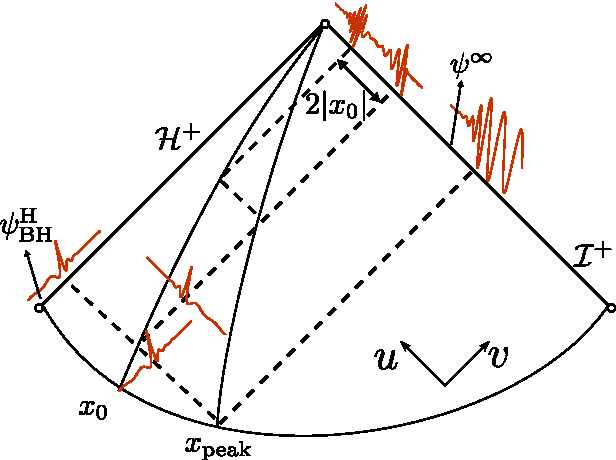
\includegraphics[width = 1.0 \columnwidth]{chapter_echo/etc/CausalDiagram.pdf}
\caption{A conformal diagram illustrating the production of echoes. The waveform that impinges on the reflecting boundary at $x_0$ is approximately the same as the waveform that reaches the horizon in the BH spacetime, $\psi^{\rm H}_{\rm BH}(v)$. Repeated partial reflections between $x_0$ and the peak of the potential $x_{\rm peak}$ result in an asymptotic waveform $\psi^\infty(u)$ made up of a main burst followed by echoes. Each echo is a reprocessed version of the waveform on the horizon $\psi^{\rm H}_{\rm BH}(v)$.}
\label{fig:CausalDiagram}
\end{figure}

We gain further insight into the nature of the additional emission by expanding $\K$ as a geometric series,
\begin{align}
\K & = \TBH \Rb e^{-2i \omega x_0} \sum_{n=1}^{\infty} (\RBH \Rb)^{(n-1)} e^{-2i(n-1)\omega x_0 } \,. \label{eq:Kgeo}
\end{align}
This shows that the additional signal takes the form of a series of terms, each reprocessing the waves that impinge on the boundary with a different transfer function. 
As we show in Sec.~\ref{sec:Echoes}, in many circumstances each term in this sequence results in a distinct pulse. 
Figure~\ref{fig:CausalDiagram} illustrates the propagation of the echoes on a conformal diagram.
The first term is the result of the primary reflection of $\psi^{\rm H}_{\rm BH}$ off of the boundary at $x_0$, which generates a factor of $\Rb $ along with a phase factor $ 2 i \omega x_0$. 
The phase factor corresponds to a time delay between the first pulse and the main burst due the pulse's extra round trip journey between the boundary at $x_0$ and the peak of the scattering potential $V$ at $x_{\rm peak}\approx 0$. 
When the pulse reaches the potential barrier, it is partially transmitted, contributing the final factor of $\TBH$.

The successive terms are ``echoes'' of this first reflection which bounce an integer number of times between the potential barrier, contributing a factor of $\RBH$, and the reflecting boundary, contributing a factor of $\Rb$, before transmitting through the potential barrier with an additional propagation delay.
Note that while the precise propagation delay of each pulse depends on the phases of $\TBH$, $\RBH$, and generically $\Rb$, the delay between echoes is constant starting with the second echo.
With this picture in mind, we define the difference between the waveform and the corresponding BH waveform to be the echo amplitude
\begin{align}
\Zecho & = \K \ZhBH \,.
\end{align}

Meanwhile, we can also consider the entire transfer function $\K$ given in Eq.~\eqref{eq:EchoTransfer}.
This function possesses its own set of resonances, and there is a complementary perspective where the waves propagating towards the reflecting boundary excite the modes of a resonant cavity between the boundary and potential barrier.
We discuss this perspective in Sec.~\ref{sec:ECOExcitation}.


\section{Examples of Echoes}
\label{sec:Echoes}

In this section we illustrate the reprocessing of the horizon waveform $\psi^{\rm H}_{\rm BH}$ using two simple examples: a spacetime with a frequency independent reflectivity $\Rb$ and a wormhole spacetime.
We show that the additional waves appear as a sequence of echoes when the boundary is far from the peak of the potential barrier, but this behavior is lost for boundaries closer to the peak.

\subsection{Individual echoes}

\begin{figure}[t]
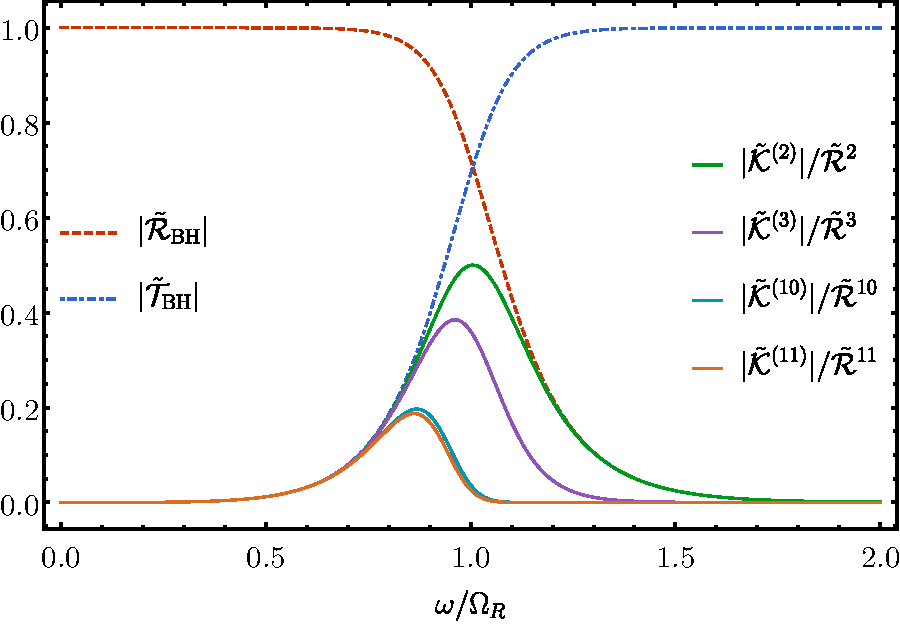
\includegraphics[width =1 \columnwidth]{chapter_echo/etc/RTK.pdf}
\caption{
The frequency domain $\ell =2$ black hole reflectivity $|\RBH|$ and transmissivity $|\TBH|$. We also plot the magnitude of the rescaled transfer functions $|\K^{(n)}|/\Rb^n$ for a boundary with constant reflectivity, for $n=2,3,10$ and $11$. 
}
\label{fig:ConstantRtransfer}
\end{figure}

The picture of successive echoes is made even more apparent by working in the time domain.
The waveform seen by distant observers is determined through $\Zref$ by
\begin{align}
\psi^\infty(u) & =  \int_{-\infty}^{\infty} \frac{d\omega}{2\pi} \Zref e^{-i\omega u} 
= \psi^{\infty}_{\rm BH}(u) + \psi_{\rm echo}(u)\,, \\
\psi_{\rm echo}(u) & \equiv \int_{-\infty}^{\infty} \frac{d\omega}{2\pi}   \K \ZhBH e^{-i\omega u}  \,,
\end{align}
where we have denoted the additional waveform due to the reflecting boundary $\psi_{\rm echo}$.
For understanding the echoes, it is useful to further split $\psi_{\rm echo}= \sum_n \psi_{\rm echo}^{(n)}$ into contributions $\psi_{\rm echo}^{(n)}$ from each term in Eq.~\eqref{eq:Kgeo} for $\K$,
\begin{align}
&\psi_{\rm echo}^{(n)}(u)  \equiv \int_{-\infty}^{+\infty} \frac{d\omega}{2\pi}\K^{(n)}\ZhBH e^{-i\omega u}  \,, \\
\label{eq:Kn}
&\K^{(n)}(\omega)\equiv(\TBH \Rb)(\RBH \Rb)^{(n-1)}e^{-2i\omega x_0 n} \,,
\end{align}
which are defined in terms of transfer functions $\K^{(n)}$ for each echo. 

In the time domain, the reflection and transmission amplitudes are given by response functions
\begin{align}
\mathcal R_{\rm BH}(t) = & \int \frac{d\omega}{2\pi} \, \RBH(\omega) e^{-i \omega t} \,,
\end{align}
and similarly for $\mathcal T_{\rm BH}(t)$, $\mathcal R(t)$, and $\mathcal{K}(t)$.

To derive the expression for the echoes, recall that multiplication of two functions $\tilde f(\omega)$ and $\tilde g(\omega)$ in the frequency domain corresponds to convolution $(f*g)$ in the time domain, where
\begin{align}
(f*g)(t) = \int_{-\infty}^{\infty} d\tau f(t - \tau) g(\tau)\,.
\end{align}
With this notation the first echo is 
\begin{align}
\psi_{\rm echo}^{(1)}(u) & = [\mathcal{K}^{(1)} *\psi^{\rm H}_{\rm BH}](u)  
\nonumber \\&
=  [(\mathcal T_{\rm BH} * \mathcal R)* \psi^{\rm H}_{\rm BH}](u + 2 x_0),
\end{align}
where $\mathcal K^{(n)}$ is the Fourier conjugate to $\K^{(n)}$, $\psi^{\rm H}_{\rm BH}$ is the Fourier conjugate to $\ZhBH$, and recall that $x_0$ is negative for boundaries near the horizon.
For the successive echoes,
\begin{align}
\psi_{\rm echo}^{(n)}(u) =&
[\mathcal{K}^{(n)} *\psi^{\rm H}_{\rm BH}](u)
\nonumber \\
=& [(\mathcal T_{\rm BH} * \mathcal R) * (\mathcal R_{\rm BH} * \mathcal R) * \dots 
\notag \\ & 
* (\mathcal R_{\rm BH} * \mathcal R) * \psi^{\rm H}_{\rm BH}](u + 2nx_0) \,. \label{eq:echon}
\end{align}
where there are $n-1$ convolutions of $(\mathcal R_{\rm BH} * \mathcal R)$ with $\psi^{\rm H}_{\rm BH}$. 


\begin{figure}[t]
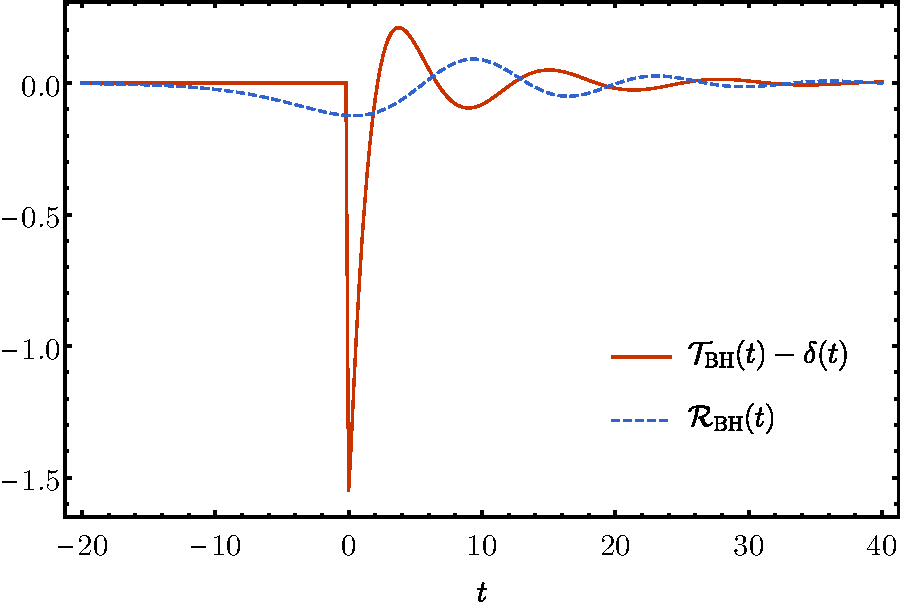
\includegraphics[width =1.0 \columnwidth]{chapter_echo/etc/TRplot}
\caption{ The $\ell =2$ scalar reflectivity and transmissivity of the potential barrier, calculated numerically in the time domain.}
\label{fig:RTtimeDom}
\end{figure}

We calculate the BH response functions $\mathcal R_{\rm BH}$ and $\mathcal T_{\rm BH}$ both in the time and frequency domain using numerical methods described in Appendix \ref{sec:RTcalc}.
The blue and red dashed curves in Fig.~\ref{fig:ConstantRtransfer} show $\RBH$ and $\TBH$ in the frequency domain for the $\ell =2$ scalar wave equation\footnote{
From their definitions,  $\TBH=1/B_{\rm out}$ and $\RBH=B_{\rm in}/B_{\rm out}$ possess resonances (poles) at the complex BH QNM frequencies \cite{Berti:2009kk}; however these resonances do not manifest themselves as clearly separated peaks on the real $\omega$ axis since the width of the QNM resonances is large compared to their spacing.
}. 
As expected \cite{Caponthesis,wheeler1972magic,Frolov:1998wf}, at low frequencies compared to the size of the potential peak $(M\omega)^2 \ll V_p$, waves are completely reflected,
\begin{align}
&|\TBH(\omega) |\to 0,& &|\RBH(\omega) |\to 1,
\end{align}
while at high frequencies $(M\omega)^2 \gg V_p$ waves are completely transmitted
\begin{align}
&\TBH(\omega) \to 1,& &|\RBH(\omega) |\to 0,
\end{align}
The transition between the two regimes occurs at approximately the real part of the $\ell = 2$ fundamental BH QNM frequency  
\begin{align}
M\Omega = M\Omega_R + i M\Omega_I \approx 0.48-0.10i \,,
\end{align}
since $V_p\approx (M\Omega_R)^2$.

Figure \ref{fig:RTtimeDom} shows $\mathcal R_{\rm BH}$ and $\mathcal T_{\rm BH}$ in the time domain. Both response functions ring down at the BH QNM frequency $\Omega$. 
As is explained in the appendix, the high frequency behavior for $\TBH$ implies that in the time domain $\mathcal T_{\rm BH}(t)$ contains a $\delta(t)$ singularity at $t=0$, which is subtracted off in the figure.

Using the echo response functions computed from $\TBH$ and $\RBH$, we now study the echo morphology from a variety of ECOs.
When presenting numerical results, we use units so that the mass of the BH spacetime is unity, $M=1$, and when we discuss a particle with scalar charge $q$ we also set $q = 1$. 


\subsection{Frequency Independent Reflectivity}
\label{sec:FIechos}

The simplest type of boundary condition in this model is a frequency independent reflectivity $\Rb$.  In this case, the echoes have a straightforward dependence on the ECO parameters $\mathcal \Rb$ and $x_0$. 
The reflectivity factors out of the response functions $\mathcal K^{(n)}$ and controls the size of each echo, without contributing any phase factors. 
Thus the majority of the time delay between echoes is due to the phase $2\omega x_0$, corresponding to a round trip journey from the potential peak near $x\approx 0$ and the boundary at $x_0$, with only  a small contribution from the BH scattering coefficient $\RBH$. 

The shape of each echo is described by the rescaled response functions
\begin{align}
\label{eq:ShiftedEchoResponse}
e^{2i\omega x_0 n}\K^{(n)}(\omega)/\Rb^n = \TBH (\omega)\RBH(\omega) ^{(n-1)} \,,
\end{align}
which we show in Fig.~\ref{fig:ConstantRtransfer}.
Recall that $|\TBH|$ is approximately zero low frequencies and approximately one at large frequencies, while the opposite is true for $|\RBH|$.
This behavior produces a small window of frequencies where the second echo response function is nonzero. 
The third echo response comes from the multiplying the second echo response function by $\RBH$; this results in a smaller slightly shifted window of frequencies. This pattern repeats with each subsequent response function. However, as the window shifts to the left, $|\RBH|\to 1$ and so the change in absolute value of the transfer functions slows, so that there is very little difference between 10th and 11th echoes.

\begin{figure}[t]
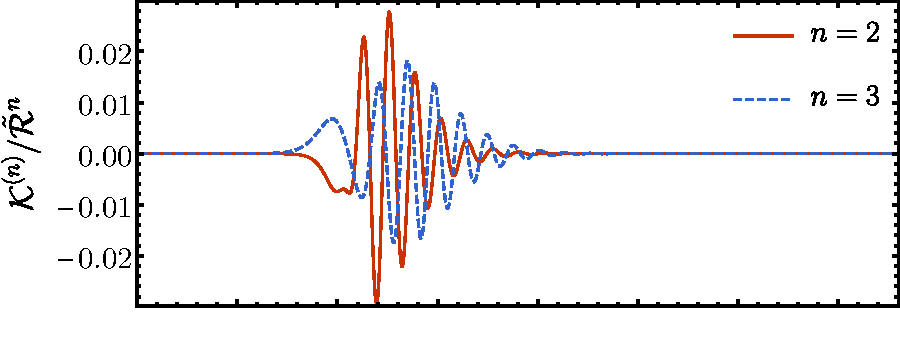
\includegraphics[width=0.98\columnwidth]{chapter_echo/etc/Kplot1.pdf}\\
\vspace{-14.5pt}
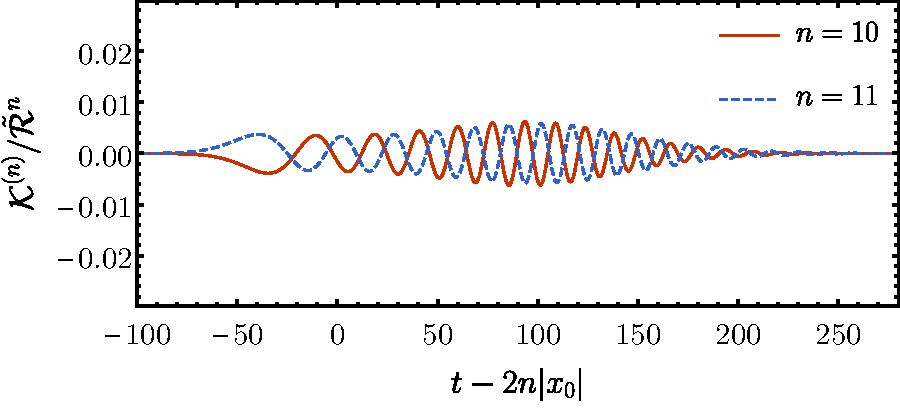
\includegraphics[width=0.98\columnwidth]{chapter_echo/etc/Kplot2.pdf}
\caption{
The constant reflectivity $\ell = 2$ echo response functions $\mathcal K^{(n)}$ for $n=2$ and 3 (top) and $n=10$ and 11 (bottom). We divide the response functions by $\Rb^n$ to rescale them and time shift each by $2 n |x_0|$ so they overlap.
}
\label{fig:Echotransfertime}
\end{figure}

In the time domain, the rescaled response functions in Eq.~\eqref{eq:ShiftedEchoResponse} are time shifted to remove the delay between echoes due to the factor of $e^{2i\omega x_0 n}$. Figure \ref{fig:Echotransfertime} shows the rescaled and shifted time domain echo response functions, obtained by numerically performing the convolutions on $\mathcal T_{\rm BH}$ and $\mathcal R_{\rm BH}$.
Each transfer function goes to zero at early times and is a decaying sinusoid at late times. The complex frequency of the sinusoid is nearly the fundamental QNM frequency $\Omega$ for the first few echoes, while for later echoes the decay time gets longer and the oscillation frequency gets slightly smaller. 

Similar trends are seen in the echoes themselves.
The waveforms at both infinity and on the horizon depend on our particular choice of sources and initial data.
As an illustration throughout this paper, we consider the echoes produced by a test particle with unit scalar charge following an orbit that we refer to as the ISCO plunge orbit. 
This orbit is a geodesic that spirals inward from the innermost stable circular orbit (ISCO), with the ISCO energy and angular momentum, and reaches the horizon at an advanced time $v_{\rm H}$. Note that for large $|x_0|$ the advanced time $v_H$ that the particle crosses the horizon in the BH spacetime is nearly equal (with corrections that scale as $\exp(x_0/2M)$) to the advanced time the particle crosses $x_0$ in the ECO spacetime.
We select this orbit since it is a reasonable model for the ringdown portion of the scalar waveform for orbits that have been circularized prior to reaching the ISCO radius, by a mechanism such as radiation reaction \cite{Hadar:2009ip}.
We use a numerical Green's function to generate the waveform from this source, which we subsequently window at early times so it smoothly starts from zero. 
Details on the entire procedure are found in Appendix~\ref{sec:Numerics}.


Since our method is to reprocess waveforms from BH spacetimes, our formalism cannot capture the emission in an actual ECO spacetime after the particle passes $x_0$.
Namely, Eq.~\eqref{eq:Gref} for $\gref$ can only be used when the source is outside $x_0$, but we use Eq.~\eqref{eq:Gref} for all source locations.
Using a particular ECO model, this additional radiation could be added directly to our waveforms, with only a small remaining inaccuracy due to the suppressed emission in our waveforms as the particle travels from $x_0$ to the horizon. 

\begin{figure}[t]
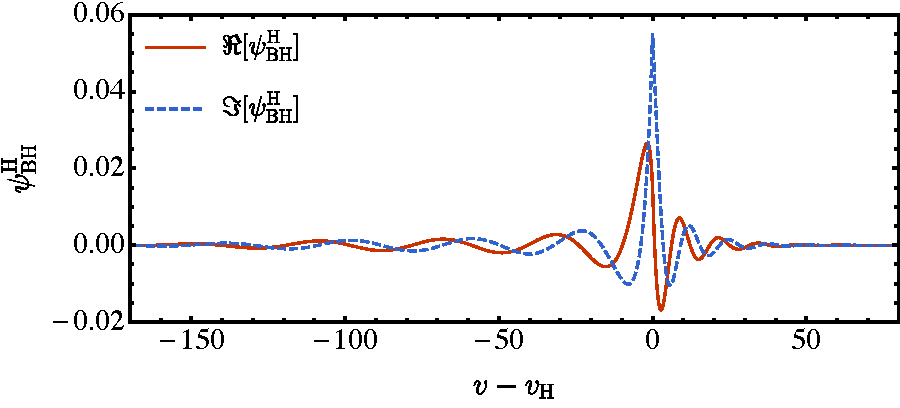
\includegraphics[width = 1 \columnwidth]{chapter_echo/etc/PsiHTD.pdf}\\
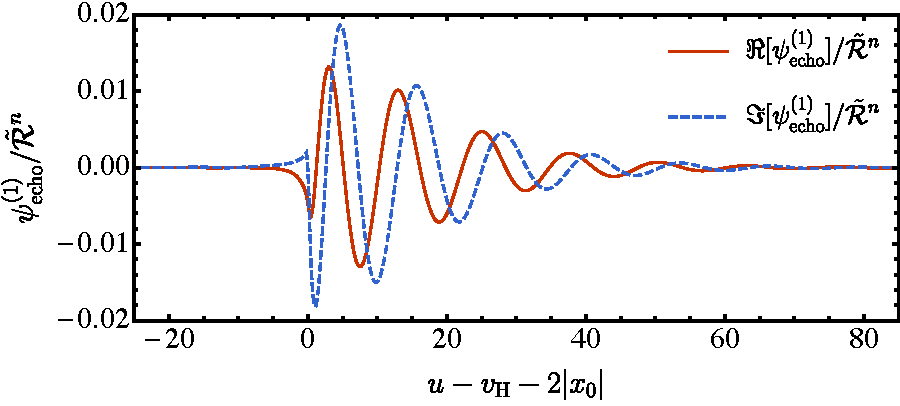
\includegraphics[width = 1 \columnwidth]{chapter_echo/etc/Echo1TD.pdf}
\caption{
Top: The $(\ell,m)=(2,2)$ waveform on the horizon $\psi_{\rm BH}^{\rm H}$, as produced by a test charge following the ISCO plunge orbit.
Bottom: The corresponding first echo $\psi_{\rm echo}^{(1)}$, rescaled and shifted in time, for a frequency-independent reflectivity.
}
\label{fig:Echotime}
\end{figure}

Figures \ref{fig:Echotime} and \ref{fig:Echotime2} show the $(\ell,m)=(2,2)$ horizon waveform and select echoes in the time domain from the ISCO plunge.
At early times the horizon waveform frequency is $\omega=m\Omega_{\rm ISCO}$, where $\Omega_{\rm ISCO}$ is the ISCO orbital frequency, and at late times there is a ringdown at the fundamental BH QNM frequency. 
The echoes also display a highly suppressed oscillation at $\omega \approx m\Omega_{\rm ISCO}$ at early times and then asymptote to decaying sinusoids at late times. 
The complex frequency of the sinusoid displays the same qualitative behavior as the echo response functions; each echo decays less than the previous and has a slightly lower frequency, with consecutive early echoes differing more than consecutive late echoes. We explore these features in more detail in Sec.~\ref{sec:Gen}.

\begin{figure}[t]
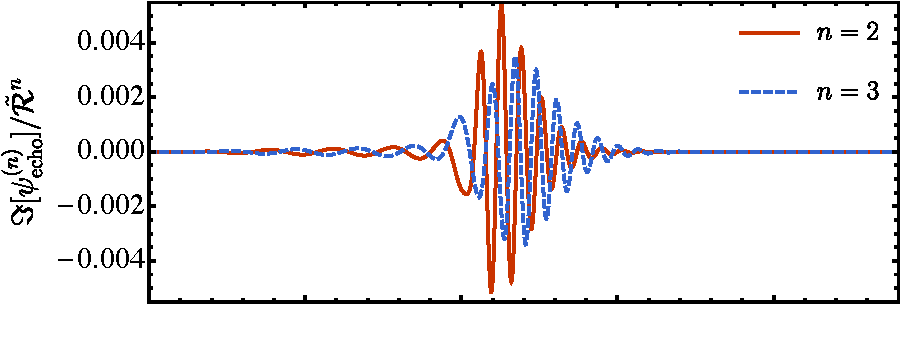
\includegraphics[width = 1 \columnwidth]{chapter_echo/etc/Echo23TD.pdf}\\
\vspace{-11.5pt}
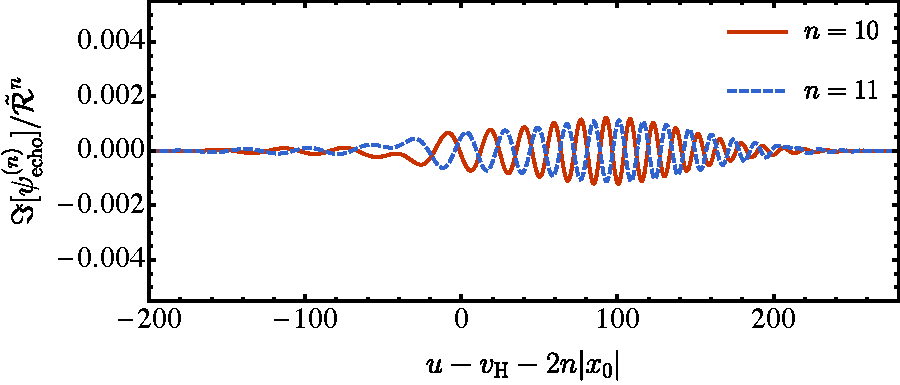
\includegraphics[width = 1 \columnwidth]{chapter_echo/etc/Echo1011TD.pdf}
\caption{
The $(\ell,m)=(2,2)$ echoes for a frequency independent reflectivity $\Rb$. The source is a test charge following the ISCO plunge orbit. We show the imaginary part of each echo, rescaled by $\Rb^n$ and shifted in time to overlap.
Top: The second and third echoes.
Bottom: The tenth and eleventh echoes. At this stage, successive echoes change only slightly in duration and amplitude.
}
\label{fig:Echotime2}
\end{figure}

\subsection{Wormhole}

The echoes from specific ECO spacetimes can also be placed within the reflecting boundary formalism.
Consider for example a wormhole produced by identifying two Schwarzschild spacetimes of mass $M$ at an areal radius $r_0$.  In Appendix \ref{sec:wormdetails}, we show that an observer in one universe can describe the influence of the other universe on wave propagation by a reflecting boundary condition $\tilde \psi \propto \Rb(\omega)e^{i\omega(x-x_0)}+e^{-i\omega (x-x_0)}$ as $x\to x_0$, where
\begin{align}
\Rb(\omega)=\RBH(\omega)e^{-2i\omega x_0} \,.
\label{eq:wormbc}
\end{align}
The free propagation phase $e^{-2i\omega x_0}$ appearing in the reflectivity accounts for the additional delay as the waves propagate to the potential peak in the other universe and back again.

Echoes in the wormhole spacetime are simply related to frequency independent $\Rb=1$ echoes. Namely the $n$th echo in the wormhole spacetime is the $2n$th echo of the $\Rb=1$ case, as can be seen from Eq.~\eqref{eq:Kn}. 
Therefore, the wormhole echoes exhibit the same patterns as the frequency-independent echoes. A comparison of the first echoes and the fifth echoes produced by a test charge following the ISCO plunge orbit is shown in Fig.~\ref{fig:eccom}.

\begin{figure}[t]
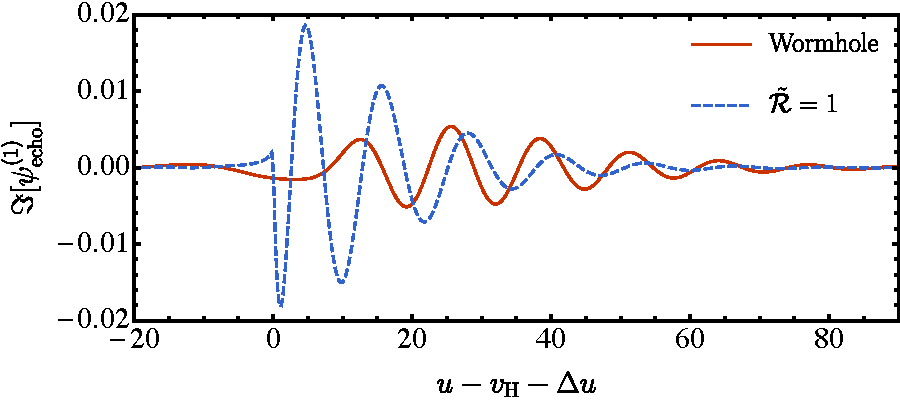
\includegraphics[width = 1 \columnwidth]{chapter_echo/etc/Wormhole1TD.pdf} \\
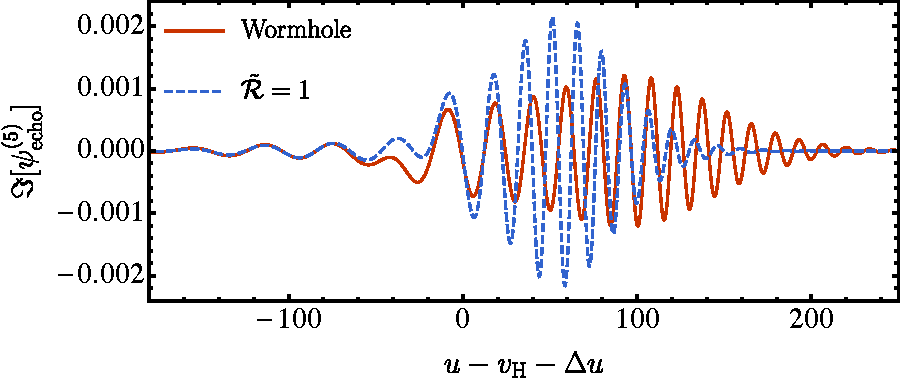
\includegraphics[width = 1 \columnwidth]{chapter_echo/etc/Wormhole2TD.pdf}
\caption{
The imaginary part of the $(\ell,m)=(2,2)$ time domain echoes  excited by a test charge following the ISCO plunge orbit in a wormhole spacetime, as compared with the echoes of the $\Rb=1$ reflecting boundary. We plot the first echo (top) and fifth echo (bottom). Each wormhole echo is shifted by $\Delta u = 4 n |x_0|$, while each constant reflectivity echo is shifted by $\Delta u = 2 n |x_0|$.
}
\label{fig:eccom}
\end{figure}

\subsection{Echo interference}

\begin{figure}[t]
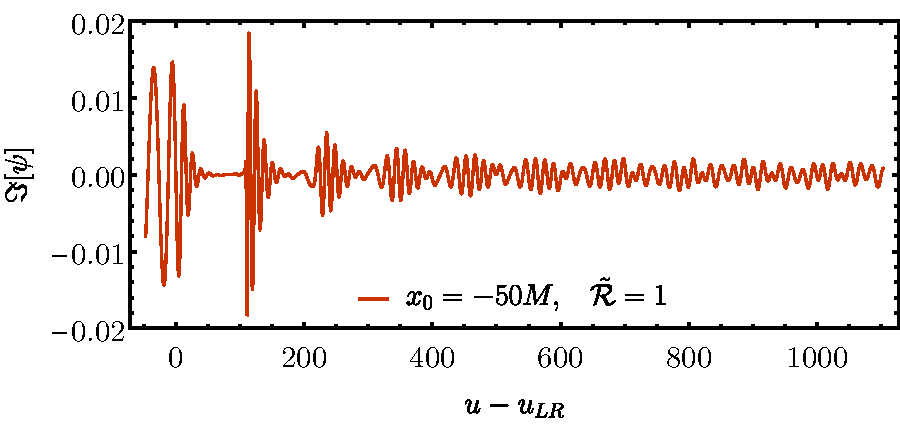
\includegraphics[width = 1 \columnwidth]{chapter_echo/etc/xW50R1plot} \\
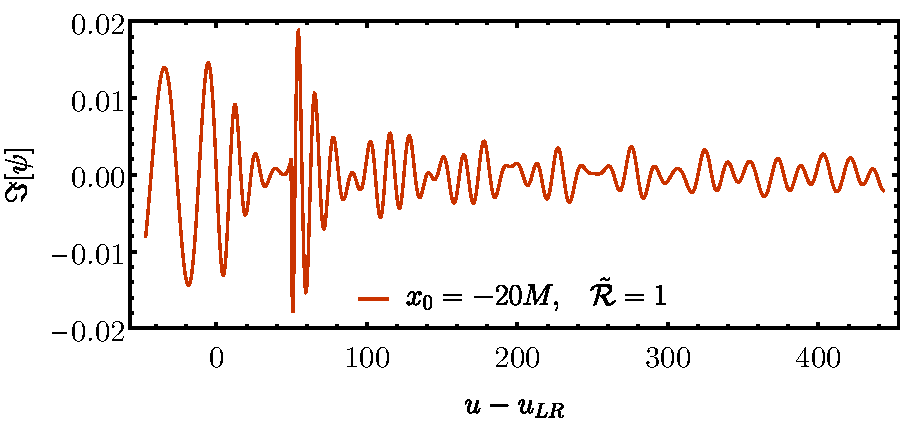
\includegraphics[width = 1 \columnwidth]{chapter_echo/etc/xW20R1plot} \\
\caption{
The imaginary part of the $(\ell,m)=(2,2)$ total  waveform $\psi^\infty$ excited by test charge following the ISCO plunge orbit. We show results for an ECO with $\Rb=1$ and $x_0 =-50 M$ (top),
and an ECO with $\Rb=1$ and $x_0 =-20 M$ (bottom). We shift the time axis by the retarded time that the charge crosses the spherical photon orbit, $u_{\rm LR}$.
}
\label{fig:Esum1}
\end{figure}

Having explored the individual echo pulses, we now examine the full echo waveform.
When the spacing between echoes is large compared to the duration of each echo, the echoes do not interfere and the total waveform appears as a sum of echo pulses. Figure \ref{fig:Esum1} shows the waveform $\psi^\infty(u)$ generated by the ISCO plunge orbit in the case $\Rb = 1$, truncating the echo sum at $n=11$. We illustrate the $\ell = 2$ waveform for two locations $x_0$ of the boundary.

The top panel shows the total waveform for $x_0=-50 M$.
The first part of the waveform is the BH waveform $\psi_{\rm BH}^\infty$, which initially oscillates at roughly a frequency of $m\Omega_{\rm ISCO}$ and transitions to ringing at the BH QNM frequencies. 
The transition occurs around a retarded time $u_{\rm LR}$, when the particle crosses the light ring.
Roughly $|2x_0|$ later, there are three to four distinct echo pulses, each spaced by roughly $|2x_0|$. 
As we observed earlier, the later echoes decay more slowly and do not appear distinct because they have a long enough duration to interfere with each other. 
The bottom panel shows the case $x_0=-20 M$, where there are only two distinct pulses before the echoes begin to interfere.

\begin{figure}[t]
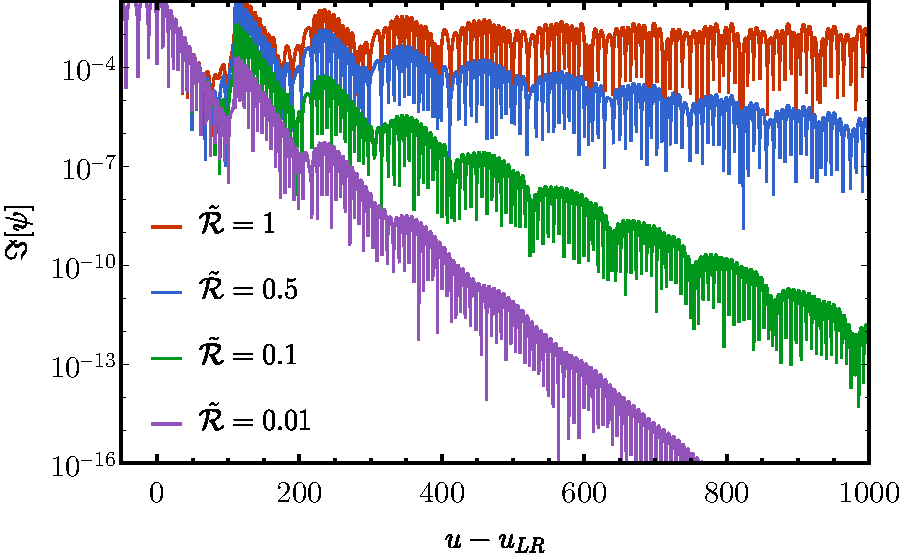
\includegraphics[width = 1 \columnwidth]{chapter_echo/etc/difrefechosumplot}
\caption{The imaginary part of the $(\ell,m)=(2,2)$ total waveform $\psi^\infty$ excited by a test charge following the ISCO plunge orbit.
We show results for ECOs with $x_0 =-50 M$ and several different choices of a frequency independent $\Rb$.}
\label{fig:EsumManyRb}
\end{figure}

We show additional examples in Fig.~\ref{fig:EsumManyRb}, using our ISCO plunge waveform. In this figure, the ECO surface is located at $x_0=-50 M$ and $\Rb$ ranges from $0.01$ to $1$. While only three to four distinct echoes are visible at large $\Rb$, for $
\Rb = 0.1$ we can see many pulses in the rapidly decaying waveform.

\begin{figure}[t]
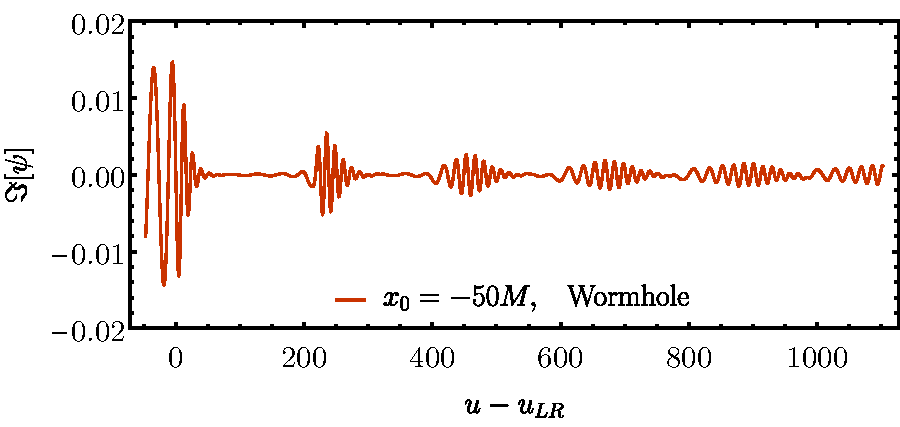
\includegraphics[width = 1 \columnwidth]{chapter_echo/etc/xW50wormplot} \\
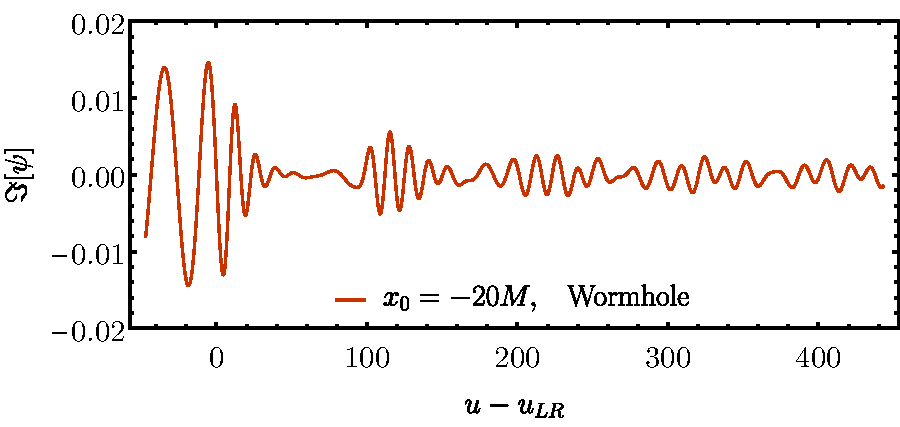
\includegraphics[width = 1 \columnwidth]{chapter_echo/etc/xW20wormplot} 
\caption{
The imaginary part of the $(\ell,m)=(2,2)$ total waveform $\psi^\infty$ excited by a test charge following the ISCO plunge orbit. We show results for a wormhole with $x_0=-50M$ (top) and $x_0=-20M$ (bottom).
}
\label{fig:EsumWormhole}
\end{figure}

The observation also holds for wormhole waveforms, which we show in Fig.~\ref{fig:EsumWormhole}.
The doubled propagation time as compared to the $\Rb = 1$ case produces a longer spacing between echoes.
As such, the early wormhole echoes are more distinct than early $\Rb =1$ echoes. 

Meanwhile, when the spacing between the echoes is small compared to the echo duration, there can be no distinct pulses. 
Instead, the waveform resembles a single decaying sinusoid at a frequency different than the BH frequency.
Figure \ref{fig:SingleECOModeTime} shows an occurrence of this for $\Rb =1$, $x_0=-3M$ and the ISCO plunge orbit.
In this case, the total waveform, appearing as the red solid curve, initially agrees with the BH waveform $\psi^\infty_{\rm BH}$, appearing as the black dotted curve, but then transitions to a decaying sinusoid. 
Note that this case pushes the limits of our approximation that the waves propagate freely near $x_0$; for $x_0 = -3M$, $r_0 \approx 2.08 M$ and $V(r_0)$ is approximately $25\%$ its peak value.

This decaying sinusoid is in fact the coherent superposition of the late echoes, a fact that we illustrate by plotting the last seven echoes appearing in the echo sum in purple. 
This coherent superposition occurs because  the later echoes all have nearly the same frequency. 
Finally note that the missing echoes from the truncated sum are not negligible compared to the total waveform, a fact we illustrate by also plotting the last echo appearing in the sum in green. 
In Sec.~\ref{sec:SingleMode} we study this example in the frequency domain, and we find that this is an example of the excitation of a single resonant mode of the ECO spacetime as described by our reflecting boundary condition.

\begin{figure}[t]
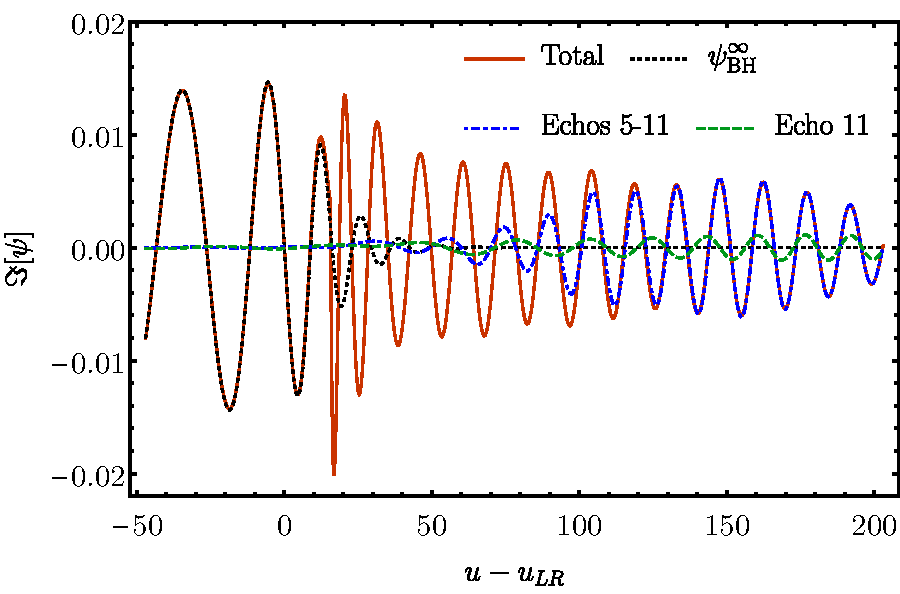
\includegraphics[width = 1 \columnwidth]{chapter_echo/etc/singlemodeplot}
\caption{
The imaginary part of the $(\ell,m)=(2,2)$, time domain, total waveform excited by a test charge following the ISCO plunge orbit. We show results from an ECO with $\Rb=1$ and $x_0 =-3M$. The total waveform is obtained by summing the black hole waveform $\psi^\infty_{\rm BH}$ and a finite number of echoes. Each curve contains a different numbers of echoes.
}
\label{fig:SingleECOModeTime}
\end{figure}

\section{Excitation of ECO Modes}
\label{sec:ECOExcitation}

The presence of the reflecting boundary condition drastically changes the spectrum of the spacetime.
The result is a different set of resonant frequencies, those of the ECO spacetime which correspond to the trapped w-modes of relativistic stars \cite{Kokkotas:1995av,Andersson:1995ez,Andersson1996wm,Benhar:1998au,Volkel:2017ofl}.
In this section we explore how our model treats these modes, and how they relate to the echoes discussed in Sec.~\ref{sec:Echoes}.

\subsection{New Modes}
\label{sec:ECOModes}

\begin{figure}[t]
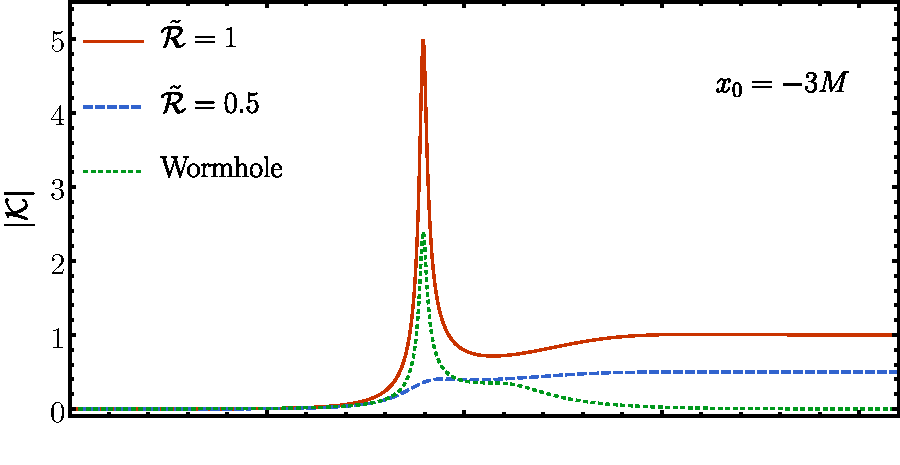
\includegraphics[width = 1 \columnwidth]{chapter_echo/etc/singlemodetransferplot}\\
\vspace{-14.5 pt}
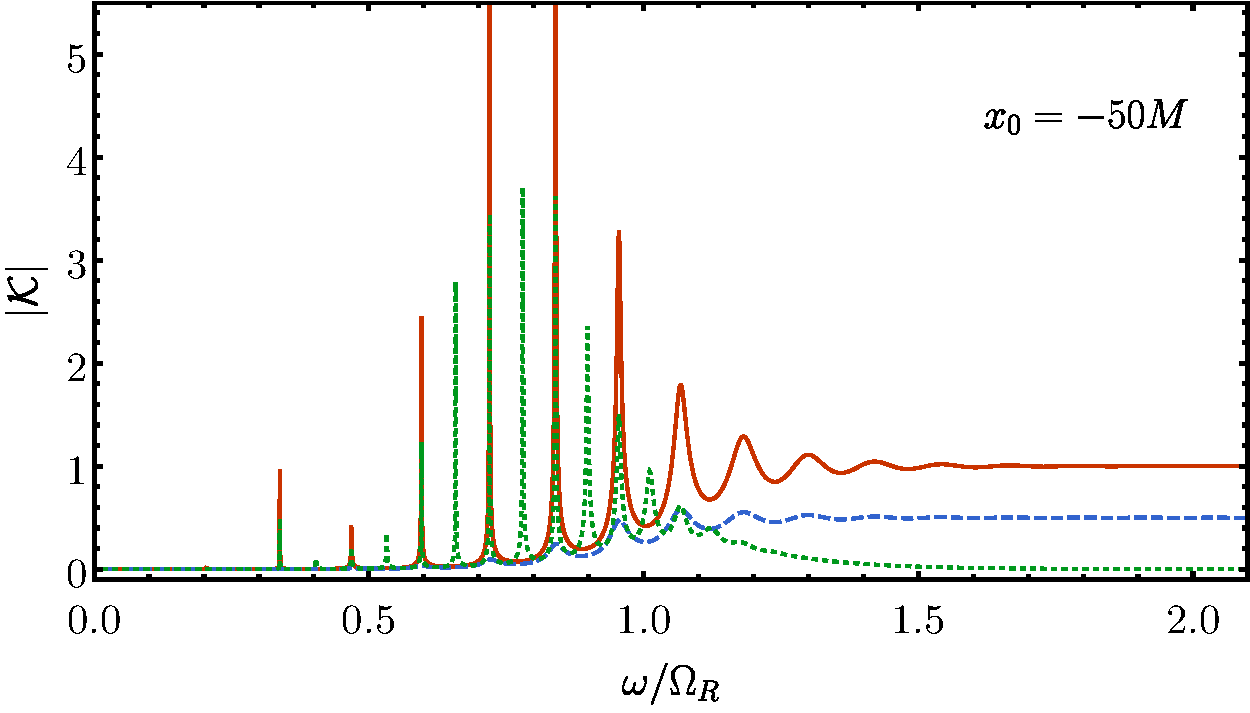
\includegraphics[width = 1 \columnwidth]{chapter_echo/etc/multimodetransferplot}
\caption{
Top: The $\ell=2$ echo transfer function $|\K(\omega)|$ for $x_0=-3M$ and several choices of $\Rb$. Note that $|\K|$ is a symmetric function of $\omega$. Bottom: The same plot for $x_0=-50M$.
}
\label{fig:NewModes}
\end{figure}

The QNM resonances are the complex poles of the Green's function.
From Eq.~\eqref{eq:gBH}, we see that for a BH, they occur when $W_{\rm BH} = 0$. 
The BH QNMs are not poles of the ECO Green's function. 
As is seen from Eq.~\eqref{eq:Gref}, the first and second terms both have poles at the QNM frequencies, but these cancel in the full expression.

The modes of the ECO spacetime come from the poles of the response function $\K(\omega)$ appearing in the Green's function,
\begin{align}
\K = \frac{\TBH \Rb e^{-2i\omega x_0}} {1 - \RBH \Rb e^{-2i \omega x_0} } \,. \notag
\end{align}
These modes obey both the reflecting boundary condition at $x_0$ as well as the outgoing wave condition at $\mathcal I^+$.
Figure \ref{fig:NewModes} shows the $|\K|$ for $\Rb =1$, $\Rb =0.5$, and for the wormhole spacetime, each for two values of $x_0$: $x_0 = -3 M$ and $x_0 = -50 M$.
In the figure, each peak of $|\K|$ represents a resonance of the transfer function\footnote{
A peak of the transfer function $\K$ on the real axis is a resonance in the sense that amplification occurs at this frequency. To show that a complex pole of the Green's function is responsible for this peak, one must examine $\K$ in the complex $\omega$ plane.
}.

Observe that in all our cases there are no new modes at large frequencies $\omega \gg \Omega_R$.
This behavior can be understood analytically. Recall that at large frequencies $\RBH\to 0$ and $\TBH \to 1$. 
This means that
\begin{align}
&\K(\omega)\to \Rb(\omega)e^{-2i\omega x_0},& &\omega \to \infty \,,
\end{align}
and the additional resonances are exactly the poles of $\Rb$.

For $x_0=-3M$, Fig.~\ref{fig:NewModes} clearly displays a single new mode at a frequency close to the fundamental QNM of a BH, for both $\Rb = 1$ and the wormhole.
In the case $\Rb=0.5$, there is a small peak in $|\mathcal K|$ at about the same frequency, although it is less visible. 
 
For $x_0=-50M$ and constant $\Rb$, there is a set of new modes with a frequency spacing of $2\pi/(2|x_0|)$, which corresponds to the inverse of the light travel time $T$ between the potential peak and the reflecting boundary. 
Meanwhile for the wormhole, there is a set of new modes and with a spacing of $2\pi/(4|x_0|)$, corresponding to approximately the inverse light travel time $T$ between the two potential peaks.
For an optical cavity, this spacing is known as the free spectral range of the cavity, 
\begin{align}
\omega_{\rm FSR} = \frac{2\pi}{T} \,.
\end{align}

To understand the resonances, we can use techniques from similar problems involving optical cavities. 
The zeros of the denominator of Eq.~\eqref{eq:EchoTransfer} contribute a set of resonances $\omega_n$ given by
\begin{align}
1=\RBH(\omega_n)\Rb(\omega_n)e^{-2i\omega_n x_0} \,. \label{eq:newre}
\end{align}
Consider first the situation that $\Rb(\omega)$ is frequency independent.
When we consider frequencies where $\RBH(\omega)$ varies slowly, we can solve Eq.~\eqref{eq:newre} by making the ansatz $\omega_n =\omega_{\rm FSR}(n+\Delta)$ and seeking a solution for $\Delta$, requiring that $|\Delta| < 1$.
In this case, there are two frequency scales in the problem: the scale $\delta \omega_{\rm BH} \equiv \RBH(n\omega_{\rm FSR})/\partial_{\omega}\RBH(n\omega_{\rm FSR})$ on which the reflectivity changes and the scale $\omega_{\rm FSR}$ on which the exponent of the exponential changes.
Since the reflectivity $\RBH(\omega)$ is approximately constant over intervals of length $\omega_{\rm FSR}$, then the ratio $\omega_{\rm FSR}/\delta \omega_{\rm BH}$ is small. 
Expanding the residual $\Delta=\Delta^{(0)}+\mathcal{O}(\omega_{\rm FSR}/\delta \omega_{\rm BH})$ in powers of $\omega_{\rm FSR}/\delta \omega_{\rm BH}$ and substituting into Eq.~\eqref{eq:newre}, one finds
\begin{align}
&1=\RBH(n\omega_{\rm FSR})\Rb e^{-2\pi i\Delta^{(0)}}+\mathcal{O}\left(\frac{\omega_{\rm FSR}}{\delta \omega_{\rm BH}}\right),
\end{align}
leading to the final expression
\begin{align}
 \frac{\omega_n}{\omega_{\rm FSR}} = n +  \frac{i}{2\pi} \ln(\Rb\RBH)+\mathcal{O}\left(\frac{\omega_{\rm FSR}}{\delta \omega_{\rm BH}}\right), \label{eq:wapprox}
\end{align}
where we use the principal branch of the logarithm.
Our ansatz is consistent provided $|\Delta^{(0)}| =|\ln(\Rb\RBH)/2\pi|<1$.
The real part of these new mode frequencies are spaced by $\omega_{\rm FSR}$ in agreement with Fig.~\ref{fig:NewModes}, and they decay provided $|\Rb|<1$.

More generally, when $\Rb(\omega)$ has frequency dependence we can often separate it into factors with fast and slow frequency dependence,
\begin{align}
\Rb(\omega) e^{-2i\omega x_0} = \hat {\mathcal R}(\omega)e^{i\omega T} \,,
\end{align}
where $\hat{\mathcal R}(\omega)$ varies appreciably over a characteristic range of frequencies $\delta \omega$ which is large compared to an appropriately redefined free spectral range $\omega_{\rm FSR}=2\pi/T$. Again, $T$ 
is approximately the round trip travel time between the potential peak and the major features in the true potential characterizing the ECO. For the wormhole, $\delta \omega = \delta \omega_{\rm BH}$ and $T=-4x_0$ is the light travel time. Provided both $\omega_{\rm FSR}/\delta \omega_{\rm BH}  \ll 1$ and $\omega_{\rm FSR}/\delta \omega \ll 1$, working to leading order, we again arrive at Eq.~\eqref{eq:wapprox} with $\hat {\mathcal R}$ replacing $\Rb$ and additional $\mathcal{O}\left(\omega_{\rm FSR}/\delta \omega\right)$ errors.

Notice also that the \rm{ECO} resonances for $\Rb = 0.5$ are broader than the $\Rb=1$ resonances, while the width of the wormhole resonances is similar to the $\Rb=1$ resonances. 
This also follows from Eq.~\eqref{eq:wapprox} since the width of the resonances is controlled by the decay rate of the new modes, which is proportional to $\omega_{\rm FSR}\ln(\Rb\RBH)$. In the low frequency regime that the new modes appear at, $\Rb\approx 1$ for the wormhole and we expect the width to be similar to the $\Rb=1$ case.

\subsection{Single Mode Excitation}
\label{sec:SingleMode}

We return to Fig.~\ref{fig:SingleECOModeTime}, where for $\Rb = 1$ and $x_0 = -3 M$ the echo waveform appears as a single decaying sinusoid which differs from the QNMs of the BH.
This behavior can be interpreted as the excitation of a single resonant mode of $\K$ by the plunge.
This is clearest in the frequency domain.

\begin{figure}[t]
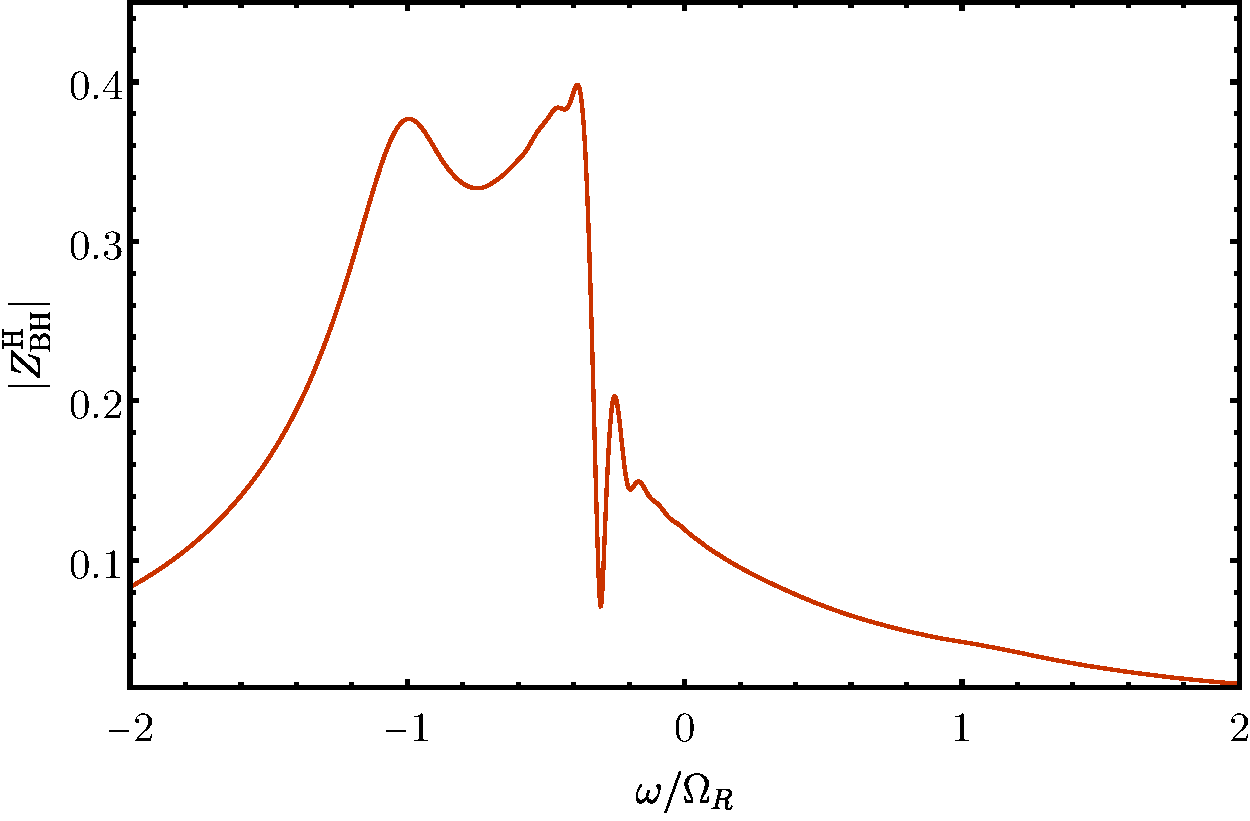
\includegraphics[width = 1 \columnwidth]{chapter_echo/etc/horizonwaveplot}
\caption{
The modulus of the $(\ell,m)=(2,2)$ horizon waveform generated by a test charge following the ISCO plunge orbit.
}
\label{fig:HorizonFT}
\end{figure}

\begin{figure}[t]
\includegraphics[width = 1 \columnwidth]{chapter_echo/etc/singlemodeFreq}
\caption{
Single mode Excitation. The $(\ell,m)=(2,2)$ response function $|\K|$, the horizon waveform $\ZhBH$ , and the echo sum $\psiecho$ for $\Rb=1$ and $x_0=-3M$. The waveforms are generated by a test charge following the ISCO plunge orbit
}
\label{fig:SingleECOModeFrequency}
\end{figure}

The excitation of the modes is encoded in the product $\Zecho=\K \ZhBH$. Figure \ref{fig:HorizonFT} displays the horizon waveform $\ZhBH$. For this orbit, most of the power is at negative frequencies and there are strong peaks near orbital frequency $\omega =-m\Omega_{\rm ISCO}$ and fundamental BH QNM frequency $\omega =-\Omega_R$. Furthermore, $\ZhBH$ goes to zero at high frequencies. 

The echo waveform $\Zecho$ is shown in Fig.~\ref{fig:SingleECOModeFrequency} for the case $\Rb=1$, $x_0=-3M$.
Note that $\Zecho$ inherits the resonance from $\K$ . 
This resonant frequency is similar to the fundamental BH QNM, but has a much slower decay, as can be noted by the slenderness of the peak compared to the peak in the horizon  amplitude at the same frequency.

\subsection{Echoes from Interference of Modes}
\label{sec:EchoInt}

Recall that for large values of $x_0$, the total waveform appears as a sum of distinct echo pulses. This scenario also can be understood in terms of the additional resonances of the ECO spacetime. 
Figure \ref{fig:MultiECOModeFrequency} shows  the frequency domain echo amplitude $\Zecho$  for three choices of $\Rb$, all with $x_0=-50M$: $\Rb=1$ appears in the top panel, $\Rb =0.5$ appears in the middle panel, and the wormhole appears in the bottom panel. 
The horizon amplitude  is substantial at all of the resonances of $\K$, which have spacing $\omega_{\rm FSR}$. 
The result is that all of the resonances appear in the $\Zecho$ in all three cases.

\begin{figure}[t]
\includegraphics[width = 1 \columnwidth]{chapter_echo/etc/R1multimodeplot.pdf}\\
\vspace{-14.75pt}
\includegraphics[width = 1 \columnwidth]{chapter_echo/etc/Rp5multimodeplot}\\
\vspace{-14.75pt}
\includegraphics[width = 1\columnwidth]{chapter_echo/etc/Rwormmultimodeplot}
\caption{
Multi-mode excitation. We fix $x_0=-50M$, a case where Fig.~\ref{fig:EsumManyRb} shows that the time domain waveform contains echoes for a range of $\Rb$. We show the $(\ell,m)=(2,2)$ response function $|\K|$, the horizon waveform $\ZhBH$, and the echo sum $\psiecho$. The waveforms ares generated by a test charge following the ISCO plunge orbit. The top panel corresponds to $\Rb=1$, the middle panel to $\Rb=0.5$, and the lower panel is the wormhole waveform.
}
\label{fig:MultiECOModeFrequency}
\end{figure}

In fact, this is what we expect a sum of echo pulses to look like in the frequency domain. Suppose that in the time domain a function $f(t)$ is a sum of delta function pulses spaced by $T=2\pi/\Delta\omega$ beginning at time $t=0$, with each pulse $\gamma$ times smaller than than the previous,
\begin{align}
\label{eq:DDcomb}
f(t)=\sum_{n=0}^\infty \gamma^n \delta\left(t-nT\right) \,.
\end{align}
Then in the frequency domain $\tilde f(\omega)$ is an infinite sum of equally spaced, equally excited resonances (see Appendix \ref{sec:DDcomb} for a derivation)
\begin{align}
\tilde f(\omega)&=\frac{i\Delta \omega}{2\pi}\sum_{n=-\infty}^\infty\frac{1}{\omega-\omega_n} \,,\nonumber \\
&\omega_n=n\Delta \omega+i\frac{\Delta \omega}{2\pi}\ln \gamma \,. 
\label{eq:DDcombFT}
\end{align}
Before the echoes begin to blend together, but after the initial BH waveform decays, the waveforms $\psi^{\infty}(u)$ shown in Figs.~\ref{fig:Esum1}, \ref{fig:EsumManyRb} and \ref{fig:EsumWormhole} are loosely of the form of $f(u)$ if we view each pulse as a delta function and choose $ T = 2|x_0|$ (or $T = 4 |x_0|$ for the wormhole case). Therefore it is not surprising that $\Zecho(\omega)$ resembles $\tilde f(\omega)$ at low frequencies, where it is more reasonable to approximate each pulse appearing in the plots by a delta function. 


\section{General Features of echoes}
\label{sec:Gen}

We turn now to some additional applications of our formalism for reprocessing black hole waveforms into waveforms from ECOs.
After reviewing some general features of echoes in our model, we develop a simple template that broadly reproduces the echoes seen by distant observers.
We also discuss the energy content of these echoes.

\subsection{General Features of echoes}
\label{sec:GFEA}

The horizon waveform $\psi^{\rm H}_{\rm BH}$ has some generic features which should hold for many sources.
Much like the inspiral, merger, and ringdown signal emitted from a compact binary, there are three phases to $\psi^{\rm H}_{\rm BH}$.
These phases are easily identifiable for the horizon waveform generated by the ISCO plunge, shown in the top panel of Fig.~\ref{fig:Echotime}.
At early times, when the small body is approximately on the ISCO orbit, the waveform frequency is approximately proportional to the ISCO orbital frequency, $\omega =m\Omega_{\rm ISCO}$. 
The waveform peaks around when the particle crosses the horizon at $v=v_{\rm H}$. At this time, there is also a discontinuity in the derivative of the waveform due to jump conditions across the particle worldline. 
At late times, after the particle has crossed the horizon, the waveform is dominated by a decaying sinusoid at the fundamental BH QNM frequency. 
These features are also seen in the frequency domain waveform shown in Fig.~\ref{fig:HorizonFT} and discussed in Sec.~\ref{sec:SingleMode}.

\begin{figure}[t]
\includegraphics[width =1 \columnwidth]{chapter_echo/etc/generalechosplot.pdf}
\caption{The modulus of the $(\ell, m) =(2,2)$ horizon waveform $Z_{\rm BH}^{\rm H}$ and select $\Rb =1$ echoes $Z_{\rm echo}^{(n)}$ generated by a test charge following the ISCO plunge orbit. Also shown are $\RBH$ ad $\TBH$.
}
\label{fig:Genechos}
\end{figure}

The ringdown has a larger effect on the shape of the first few echoes than the earlier parts of $\psi^{\rm H}_{\rm BH}$, because the fundamental QNM frequency is transmitted more easily through the potential barrier.
Meanwhile, the horizon waveform at early times, which is generally at lower frequencies associated with the inspiral orbital timescale, mostly reflects off of the inside of the potential barrier and contributes less to the first echo. The later echoes, having already lost power at frequencies near $\omega =\Omega_R$ from each earlier scatter off of the potential barrier, depend more intricately on the details of the horizon waveform at early times.

We illustrate this in Fig.~\ref{fig:Genechos}, which examines echoes from the ISCO plunge for constant reflectivity $\Rb$.
Figure \ref{fig:Genechos} shows the frequency domain horizon waveform $\ZhBH$ as well as three echoes $\Zecho^{(n)}$, where 
\begin{align}
\label{eq:nZecho}
Z_{\rm echo}^{(n)}=\K^{(n)}\ZhBH
\end{align}
are the Fourier conjugates of the $n$th echoes $\psi_{\rm echo}^{(n)}(u)$.
The first echo inherits the peak of $\ZhBH$ near $\Omega_R$, but the peak near $m\Omega_{\rm ISCO}$ is removed by $\TBH$.
The third echo similarly retains a peak near $\omega =-\Omega_R$, although shifted to a slightly lower frequency compared to the first, and is significantly narrower.
By the tenth eleventh echoes, the differences between successive echoes has become small, and the echoes retain a suppressed peak near (but to the right of) $\omega = - \Omega_R$. 
Overall, we see that because of the low frequency suppression in all the echoes, the ringdown portion of the horizon waveform is most important for determining the shape of the first several echoes.

\subsection{Template for echoes}

The observation that the ringdown of the horizon waveform $\psi^{\rm H}_{\rm BH}$ is the most important factor for determining the shape of the echoes leads to a simple idea for a template for the echoes. 
Construct a template  $Z_{\rm T}^{\rm H}$ for the horizon waveform $\ZhBH$ consisting of only a ringdown at the fundamental QNM frequency. Then construct a template $Z_{\rm T}$  for the echoes  $Z_{\rm echo}$ and a template $Z_{\rm T}^{(n)}$ for each echo $Z_{\rm echo}^{(n)}$ using the transfer functions
\begin{align}
 &Z_{\rm T}=\K Z_{\rm T}^{\rm H}\,, &
 &Z_{\rm T}^{(n)}=\K^{(n)}Z_{\rm T}^{\rm H} \,.
\end{align}

To model the ringdown of the horizon waveform, we take a superposition of decaying sinusoids that each are excited at a slightly different time.
In the time domain our template for the horizon waveform is
\begin{align}
\psi^{\rm H}_{\rm T}(t)&=(\psi_{\rm QNM}*h)(t) \nonumber \\
h(t)&=\frac{\beta}{\sqrt{2\pi}}\exp\left(\frac{-(t-t_s)^2}{2/\beta^2}\right) \nonumber \\
\psi_{\rm QNM}(t)&=\theta(t)\left(-i\alpha_+ e^{-i\Omega_+ t}-i\alpha_- e^{-i\Omega_- t}\right),
\end{align}
where we use $\psi_{\rm T}^{\rm H}$ to indicate the Fourier conjugate of $Z_{\rm T}^{\rm H}$. 
We weight each decaying sinusoid by the Gaussian $h(t)$. 
The template is parametrized by two complex amplitudes $\alpha_\pm$ for the sinusoids at the positive and negative QNM frequencies, $\Omega_\pm=\pm \Omega_R +i\Omega_I$, a central start time $t_s$, and a frequency width $\beta$. 
In the frequency domain, the template for the horizon waveform takes the even simpler form
\begin{align}
Z^{\rm H}_{\rm T}(\omega; \vec p)=e^{i\omega t_s}e^{-\omega^2/(2\beta^2)}\left(\frac{\alpha_+}{\omega-\Omega_+}+\frac{\alpha_-}{\omega-\Omega_-}\right),
\end{align}
where $\vec p=(\alpha_+,\alpha_-,t_s, \beta)$ are the template parameters.

To evaluate the template we investigate its ability to match both individual echoes and complete waveforms produced from a test charge following the ISCO plunge orbit, in the case of a constant $\Rb$.
To quantify the match, we define the overlap of two waveforms as
\begin{align}
\label{eq:overlap}
\rho^2(Z_1, Z_2)=\frac{|\braket{Z_1|Z_2}|^2}{\braket{Z_1|Z_1}\braket{Z_2|Z_2}} \,,
\end{align}
in terms of the inner product
\begin{align}
\braket{a|b}=\int_{-\infty}^\infty \frac{d\omega}{2\pi}\tilde a^*(\omega)\tilde b(\omega) \,.
\end{align}
The overlap satisfies $0 \leq \rho \leq 1$, with $\rho \approx 1$ indicating a good match.

\begin{figure}[t]
\includegraphics[width = 1 \columnwidth]{chapter_echo/etc/rhovsechonumberV2}
\caption{ The overlap $\rho(Z_{\rm T}^{(n)}, Z_{\rm echo}^{(n)}; \vec p_1)$ for the $n$th individual echo  plotted versus echo number $n$. 
The parameters $\vec p_1$ are determined by maximizing the overlap for the first $n=1$ echo. We show results for $(\ell,m)=(2,2)$ and use a test charge following the ISCO plunge trajectory as a source for the $Z_{\rm echo}^{(n)}$.
}
\label{fig:rho2vsecho}
\end{figure}

For our first test of the model, we consider the overlap for the individual echoes, $\rho(Z_{\rm T}^{(n)},\Zecho^{(n)}; \vec p)$. 
Note that the overlap for the individual echoes is independent of $x_0$ and $\Rb$.
We set the template parameters $\vec p =\vec p_1$ by analytically maximizing the overlap over $\alpha_\pm$ \cite{Zimmerman:2011dx} at fixed nonlinear model parameters $t_s$ and $\beta$; we then numerically search for optimal parameters $t_s$ and $\beta$.
We compute the overlap for successive echoes using the same fixed $\vec p_1$.

In Fig.~\ref{fig:rho2vsecho}, 
we plot $\rho(Z_{\rm T}^{(n)},\Zecho^{(n)}; \vec p_1)$
versus $n$ for the first twenty echoes. 
We see that the overlap is approximately between $0.96$ and $0.97$ and asymptotes to a constant as the echo number $n$ grows. 
We show a direct comparison of the template and the first echo in Fig.~\ref{fig:dirTemcompEchos} to give an example of the type of match produced by an overlap in this range\footnote{
Note that our procedure does not completely fix the parameters $\alpha_\pm$ since the normalized overlap is invariant under shifts $Z_{\rm T}^{(n)}\to a Z_{\rm T}^{(n)}$ for any complex constant $a$. To completely fix the parameters for Figs.~\ref{fig:dirTemcompEchos} and \ref{fig:horizonmatch}, we also impose the constraints $\braket{Z_{\rm T}^{(n)}|Z_{\rm T}^{(n)}}=\braket{Z_{\rm echo}^{(n)}|Z_{\rm echo}^{(n)}}$ and ${\rm ph}(\braket{Z_{\rm T}^{(n)}|Z_{\rm echo}^{(n)}})=0$. This is equivalent to minimizing the least squares differences between the waveforms while holding $\braket{Z_{\rm T}^{(n)}|Z_{\rm T}^{(n)}}$ constant.
}. 
Importantly, this analysis shows that the first echo can be used to generate values of the template parameters that produce reasonably good overlaps for later echoes. 

\begin{figure}[t]
\includegraphics[width = 1 \columnwidth]{chapter_echo/etc/echo1matchReV2}\\
\vspace{-14.5 pt}
\includegraphics[width = 1 \columnwidth]{chapter_echo/etc/echo1matchImV2}
\caption{ A comparison of the $(\ell, m) =(2,2)$ real (top) and imaginary (bottom) parts of the $n=1$ echo template $Z_{\rm T}^{(1)}$  and the first echo. The echo is generated by a test charge following the ISCO plunge orbit and the parameters for the template are determined by maximizing the overlap $\rho$ given by Eq.~\eqref{eq:overlap} between the template and the echo. The value of the overlap is $\rho=0.969$.
}
\label{fig:dirTemcompEchos}
\end{figure}

It is insightful to compare these overlaps to the corresponding overlap
$\rho(Z_{\rm T}^{\rm H},Z_{\rm BH}^{\rm H}; \vec p_1)$ between the horizon waveform and its template at the same parameters $\vec p_1$. 
This overlap is $\rho = 0.72$, and it is smaller than the overlap for the individual echoes. 
A direct comparison of the horizon waveform and its template, shown in Fig.~\ref{fig:horizonmatch}, reveals that the template misses key features of the horizon waveform at low frequencies $|\omega| < \Omega_R$.  
We explain the enhanced performance of the template for the echoes compared to the horizon waveform as being due to the echo transfer functions $\K^{(n)}$, which filter out the low frequencies where the template performs poorly.

\begin{figure}[t]
\includegraphics[width = 1 \columnwidth]{chapter_echo/etc/horizonmatchV2}
\caption{A comparison of the modulus of the $(\ell, m) =(2,2)$ of the horizon waveform template $Z_{\rm T}^{\rm H}$ and numerically computed horizon waveform. The waveform is generated by a test charge following the ISCO plunge orbit and the parameters for the template are determined by maximizing the overlap $\rho$ between the first echo template and the numerically calculated first echo. The value of the overlap is $\rho=0.72$.
}
\label{fig:horizonmatch}
\end{figure}


To investigate how the template models the full echo amplitude $\Zecho$, we investigate the overlap $\rho(Z_{\rm T},\Zecho;\vec p)$.
Note that this overlap does depend on $x_0$ and $\Rb$.
We fix $x_0$ and $\Rb$ and maximize over the template parameters $\vec p$. 
The results are shown in Fig.~\ref{fig:rho2Allecho} for $x_0= -3M, -20M$, and $-50M$ at several values of $\Rb$
ranging from $0.01$ to 1. 

We see that the overlap is generally greater than $0.96$ for $\Rb<0.99$. 
For $\Rb\geq 0.99$, the overlap for the larger values of $x_0$ drops significantly. 
The dramatic reduction in the overlap occurs because the amount of power (as determined by the power density $dP/d\omega=|\Zecho|^2$) in the echo waveform at low frequencies significantly increases as $\Rb\to 1$ when $x_0$ is large.
This power is contained in the narrow resonances appearing in Fig.~\ref{fig:MultiECOModeFrequency}. 
This degrades the overlap because the template is only designed to perform well for frequencies near the BH QNM frequency $\Omega_R$. 
For example when $x_0 =-50M$ and $\Rb=0.999$, less than $8\%$ of the power is at frequencies $|\omega | < 0.6\Omega_R$, while when $\Rb=1$, the number jumps to $35\%$.

\begin{figure}[t]
\includegraphics[width = 1 \columnwidth]{chapter_echo/etc/AllEchosrho}
\caption{ The overlap $\rho$ for the $(\ell,m) =(2,2)$ echo sum $Z_{\rm echo}$ for select values of $x_0$ and and $\Rb$. The waveform is generated by a test charge following the ISCO plunge orbit. The template parameters $\vec p$ are fixed in each case by maximizing the overlap for the corresponding parameters.
}
\label{fig:rho2Allecho}
\end{figure}

\subsection{Energy in the echoes}

Our formalism also allows us to relate the energy in the ECO waveform to the energy in the BH waveforms on the horizon $\mathcal{H}^+$ and at asymptotic infinity $\mathcal{I}^+$. For very compact ECOs, we derive a simple relationship between the energy in the black hole waveform and the energy in the ECO waveform.

The stress energy tensor for the scalar field is $T_{\mu\nu}=\nabla_\mu \phi\nabla_\nu \phi-(1/2) g_{\mu \nu}\nabla^\rho\phi\nabla_\rho\phi$ and energy flow is governed by the energy flux vector $-T_{\mu\nu}(\partial/\partial t)^\nu$. 
Given a wave $\psi(v)$ that impinges on the horizon or a wave $\psi(u)$ that is incident on $\mathcal{I}^+$, the energy $\mathcal{E}[\psi]$ is the functional
\begin{align}
\mathcal{E}[\psi]&=\sum_{\ell m} E_{\ell m}[\psi], \\
E_{\ell m}[\psi]&=\int_{-\infty}^\infty d\tau |\dot\psi_{\ell m}(\tau)|^2 
=\int_{-\infty}^\infty \frac{d\omega}{2\pi} \omega^2|Z_{\ell m}(\omega)|^2,
\end{align}
where we have temporarily restored the harmonic indices. The last equality is an application of Parseval's theorem, and we have denoted $Z_{lm}$ as the Fourier conjugate of $\psi_{lm}$. 

The energy of the ECO waveform $E^\infty$ can be expressed in terms of the energy in the black hole waveform  $E_{\rm BH}^\infty=E[\psi_{\rm BH}^\infty]$, the energy in the echoes $E_{\rm echo}=E[\psi_{\rm echo}]$, and correlations between the echoes and the black hole waveform
\begin{align}
 E[\psi_{\rm BH}^\infty]&=E[\psi_{\rm BH}^\infty +\psi_{\rm echo}] \nonumber \\ 
 &= E_{\rm BH}^\infty + E_{\rm echo}
+2\Re
\left[\int_{-\infty}^\infty d\tau \, \dot \psi_{\rm BH}^\infty(\tau)\dot \psi_{\rm echo}(\tau)^*\right] \,.
\end{align}

In the limit that $x_0$ is much larger than the duration of each echo, the different echoes do not overlap, allowing us to neglect the correlations, so that
\begin{align}
 E^\infty \approx E_{\rm BH}^\infty + E_{\rm echo} \label{Eq:ennocor}.
\end{align}
An identical argument allows us to write the echo energy as an approximate sum of the energy in each echo. 
\begin{align}
E_{\rm echo}& \approx \sum_{n=1}^\infty E[\psi_{\rm echo}^{(n)}] 
= \sum_{n=1}^\infty \int \frac{d\omega}{2\pi}\omega^2|\Zecho^{(n)}|^2
\nonumber \\
&= \int\frac{d\omega}{2\pi}|\Rb \TBH|^2\sum_{m=0}^\infty |\Rb\RBH|^{2m}\omega^2|\ZhBH|^2
\nonumber \\
&= \int \frac{d\omega}{2\pi}\frac{|\Rb\TBH|^2}{1-|\Rb \RBH|^2}\omega^2 |\ZhBH|^2 \,,
\label{eq:KeyEnergy}
\end{align}
where we have used Eqs.~\eqref{eq:Kn} and \eqref{eq:nZecho}.

When $\Rb =1$, since $|\TBH|^2=1-|\RBH|^2$, the echo energy $E_{\rm echo}$ is precisely the energy $E_{\rm BH}^{\rm H}=E[\psi_{\rm BH}^{\rm H}]$ that would have gone down the horizon in the BH spacetime. 
When $|\Rb|<1$, there will be less energy in the echoes than the horizon waveform, falling to $0$ as $\Rb \to 0$. 
Finally, Eq.~\eqref{eq:KeyEnergy} predicts that for very compact ECOs, the relationship between the energy in the ECO waveform and BH waveforms on $\mathcal{H}^+$ and $\mathcal{I}^+$ is independent of $x_0$.

\begin{figure}[t]
\includegraphics[width = 1 \columnwidth]{chapter_echo/etc/EnergyPlot}
\caption{
The energy $E_{\rm echo}$ in the $(\ell,m)=(2,2) $ component of the echo waveform compared to energy $E_{\rm BH}^{\rm H}$ in the horizon waveform for different values of $\Rb$ and $x_0$.  The waveforms come from a test charge following an ISCO plunge orbit.
}
\label{fig:Energy}
\end{figure}

Figure \ref{fig:Energy} shows $E_{\rm echo}/E_{\rm BH}^{\rm H}$ for $(\ell, m)=(2,2)$ waveforms from the ISCO plunge orbit for a variety of $\Rb$ and $x_0$. As expected, smaller values of $\Rb$ produce echoes containing less energy and the ratio becomes independent of $x_0$ as $x_0\to \infty$. 
For perfectly reflecting, extremely compact ECOs with $x_0>20M$, more than $97\%$ of the energy in the horizon waveform is radiated in the echoes.


\section{Conclusions}

In this work, we derive a relationship between the Green's functions for a massless scalar field in a BH spacetime and in the exterior region of ECOs.
This is accomplished by replacing the compact object with a reflecting boundary near the horizon of the BH. 
The exterior of any ECO can be modeled with a particular choice of boundary location and frequency dependent reflectivity.

We use the relationship between Green's functions to show that the ECO waveform seen by asymptotic observers is the same as that seen in the BH spacetime, plus additional emission from reflection off the boundary.
This additional emission can be computed by reprocessing the horizon waveform in the BH spacetime using a simple transfer function.
We find that the difference between the BH and ECO waveforms at infinity can be understood either as a superposition of echo pulses or a superposition of modes associated with poles in the ECO Green's function. 
Furthermore, we show how both the individual echoes and the new mode frequencies encode the information describing the ECO model; namely the boundary reflectivity and location.

Our formalism also explains how the BH QNMs imprint themselves in ECO waveforms: The ECO waveform has a main burst that rings down at the black hole QNM frequencies. 
In addition, the frequency content of the individual echo pulses is largely determined by the frequency content in the horizon waveform $\psi^{\rm H}_{\rm BH}$ near the BH QNM frequencies.
Despite the imprint of these frequencies on the ECO waveform, our formalism also shows that the BH QNM frequencies are not poles in the ECO Green's function. Rather, the piece of the Green's function responsible for producing the main burst and the piece responsible for the echoes both have poles at the BH QNM frequencies, which cancel in the full expression. 

We demonstrate how our formalism can be used to reprocess a black hole waveform into an ECO waveform by studying the echoes produced by a test charge spiralling in from the ISCO. We use our numerical results and analytic observations to design a simple template for the echoes that accurately reproduces our waveforms, with normalized overlaps $\rho > 0.95$ for most values of boundary location and reflectivity (taken here to be frequency independent). 

To determine the significance of our proposed template, future work will be required to extend the formalism to gravitational perturbations of Kerr. 
In addition to the added algebraic complexity, one will have to overcome the absence of Birkhoff's theorem in Kerr, as well as the lack of a simple scheme for parameterizing reflecting boundary conditions for gravitational perturbations \cite{Price:2017cjr} (see \cite{Nakano:2017fvh} for one possible prescription). 
Ideally, future work will also extend the formalism beyond test particle sources, so that comparable mass binaries can be treated. 
Nevertheless, our results indicate that a relatively simple template, combined with a prescription for reprocessing waveforms generated in black hole spacetimes, can be used to investigate the existence of ECOs and their echoes using gravitational wave observations.

\section{acknowledgments}
We thank Vitor Cardoso, Baoyi Chen, Chad Galley, Davide Gerosa, Yiqiu Ma, David Nichols, Samaya Nissanke, Paolo Pani, Leo Stein, Saul Teukolsky, and Huan Yang for valuable discussions. 
We are grateful to Ofek Birnholtz, Vitor Cardoso, Gaurav Khanna, Hiroyuki Nakano, and Paolo Pani for providing feedback on a draft of this manuscript. The figures were made using the MaTeX package \cite{matex}. This research was supported at Caltech by NSF grant PHY-1404569, the Walter Burke Institute for Theoretical Physics, and the David and Barbara Groce startup fund.

\section{Appendix: Calculation of the reflection and transmission coefficients}

\label{sec:RTcalc}

In this appendix we describe our calculation of the reflection and transmission coefficients $\mathcal R_{\rm BH}$ and $\mathcal T_{\rm BH}$, in both the time and frequency domains.

\subsection{Time Domain}

The scattering coefficients $\RBH$ and $\TBH$ are defined from the frequency domain solution $\psiupA$ to Eq.~\eqref{eq:RW}. 
An equivalent time-domain definition is found in terms of a solution $\psi$ to the characteristic initial value problem 
\begin{align}
\frac{\partial^2 \psi}{\partial u \partial v}+\frac{fV}{4}\psi= 0 \label{eq:psiwave}
\end{align}
with characteristic initial data posed on the past horizon $\mathcal{H}^-$ and past null infinity $\mathcal{I}^-$ consisting of a delta function pulse
\begin{align}
&\left. \psi(u)\right |_{\mathcal{H}^-} =\delta (u),& &\left. \psi(v)\right |_{\mathcal{I}^-}=0
\end{align}
as shown in Fig.~\ref{fig:RTDom}.
Then $\mathcal T_{\rm BH}(u)$ is the field $\psi(u)|_{\mathcal{I}^+}$ evaluated at future null infinity and $\mathcal R_{\rm BH}(v)$ is the field $\left. \psi(v)\right |_{\mathcal{H}^+}$ evaluated on the future horizon.
This is seen as follows.

\begin{figure}[t]
\includegraphics[width = 1 \columnwidth]{chapter_echo/etc/RTDomains}
\caption{
A Penrose diagram illustrating the relevant surfaces of the characteristic initial value definition of $\mathcal T_{\rm BH}$ and $\mathcal R_{\rm BH}$. 
Initial data, consisting of a delta function pulse at $u=0$ (red line), is posed on $\mathcal{H} ^-$ and $\mathcal{I}^-$. The transfer function $\mathcal T_{\rm BH}$ is extracted off of $\mathcal{I}^+$ and $\mathcal R_{\rm BH}$ is extracted off of $\mathcal{H} ^+$. The blue dashed lines approximately bound the near-horizon and far-field regions where $V\approx 0$. 
}
\label{fig:RTDom}
\end{figure}

When $V=0$, the general solution to Eq.~\eqref{eq:psiwave} is a superposition of an outward traveling wave and an inward traveling wave, 
\begin{align}
\psi(v,u)=h(u)+k(v) \label{eq:wavegen},
\end{align}
where $h$ and $k$ are free functions.
The potential can be neglected, $V\approx 0$, in the near horizon region, roughly bounded by the left blue dashed line in Fig.~\ref{fig:RTDom}, and also in the far field region, roughly bounded by the right blued dashed line. We match the general solution Eq.~\eqref{eq:wavegen} to the boundary data in these regions to obtain 
\begin{align}
\psi(v,u)=\begin{cases}
\delta(u)+\left. \psi(v)\right |_{\mathcal{H}^+}, & x \to -\infty \,, \\
\left. \psi(u)\right |_{\mathcal{I}^+}, & x \to \infty \,.
\end{cases}
\end{align}
Notice the field on the horizon is not determined by the initial conditions in the near horizon matching region. 
Likewise the field at future null infinity is not determined by the initial conditions in the far-field matching region. 
Calculating these fields requires all of the initial data.

Rewriting the solution in $(t,x)$ coordinates and taking the Fourier transform with respect to $t$ yields
\begin{align}
\tilde \psi(\omega,x)
&=\begin{cases}
e^{i\omega x}+\ \tilde \psi(\omega) |_{\mathcal{H}^+}e^{-i\omega x}, & x \to -\infty \\ \tilde \psi(\omega) |_{\mathcal{I}^+}e^{i\omega x}, & x \to \infty.
\end{cases}
\end{align}
Comparing this with frequency domain definition Eq. ~\eqref{eq:RTAmplitudes} of $\mathcal R_{\rm BH}$ and $\mathcal T_{\rm BH}$, we identify 
\begin{align}
\tilde \psi(\omega)|_{\mathcal{H}^+} &= \RBH(\omega) \,, \\ \tilde \psi(\omega)|_{\mathcal{I}^+} &= \TBH(\omega) \,,
\end{align}
establishing the equivalence of the two definitions.

For our numerical calculations, it is important to realize that $\mathcal T_{\rm BH}(u)$ only has support for $u\geq 0$ and $\mathcal T_{\rm BH}(0)=\delta(0)$. The first fact follows from $\psi(v,u)=0$ for $u<0$, since for these times $\psi$ lies in the domain of dependence of the portion of initial data which is equal to zero. 
The second conclusion follows from the high frequency behavior $\TBH\to 1$ as $\omega/\Omega_R \to \pm\infty$ \cite{Caponthesis}. This implies that $\TBH = 1 + f(\omega)$, where $f\to 0$ as $\omega \to \pm \infty$. Taking the Fourier transform of both sides gives the delta function at $u=0$. 

We use our characteristic code for homogeneous solutions to wave equations detailed in Sec.~\ref{sec:charcode} to solve this characteristic initial value problem.
Namely, we pose the initial data on the future part of a null cone described by $v=v_0$ and $u=0$ and choose $-v_0$ large enough that the delta function pulse $\delta(u)$ is deep in the near horizon region. 
We use a discrete approximation for the delta function in the initial data  
\begin{align}
\delta(u) =\begin{cases}
\displaystyle
\frac{1}{2(2h)}, & u =0 \\
0, & \text{otherwise}
\end{cases}.
\end{align}
where our numerical grid is spaced by $2h$.
We extract $\mathcal R_{\rm BH}$ off of the ray $u=u_E$ in our computational domain that is closest to $\mathcal{H}^+$. 
Similarly we extract $\mathcal T_{\rm BH}$ off of the ray $v=v_E$ in our computational domain that is closest to $\mathcal{I}^+$.

We performed convergence checks on our choice of stepsize $h$, initial data ray location $v_0$ and the location of the extraction rays $v_E$ and $u_E$. 
We used $h =0.025M$. 
We verified that the same numerical approximation of the $\delta(u)$ that we used in our initial data appears in $\mathcal T_{\rm BH}$. 
For calculations in the paper that rely on $\mathcal T_{\rm BH}$, we insert the $\delta$ function analytically and only use the smooth part of $\mathcal T_{\rm BH}$ from our code.
To obtain the smooth part of $\mathcal T_{\rm BH}(u)$ near zero we extrapolated this data backwards in time a single time step.

\subsection{Frequency Domain}

For computations that required accurate frequency domain representations of $\RBH$ and $\TBH$, we also computed  $\RBH$ and $\TBH$ directly in the frequency domain. This also provided an independent check of our time domain methods. 

At a fixed frequency, the homogeneous wave equation \eqref{eq:RW} together with one of the two boundary conditions in Eq.~\eqref{eq:psiup} forms a boundary value problem for  $\psiupA(\omega, x)$. The coefficients $B_{\rm out}$ and $B_{\rm in}$ necessary to compute  $\RBH$ and $\TBH$ are determined from the solution and its derivative near the opposite boundary by comparing to the remaining boundary condition. 

We numerically integrated outward from the horizon, using an analytic third-order expansion of $\tilde \psi$ to match the boundary condition there.
We extracted the field at a large radius $r = 1000M$, matching to an asymptotic expansion of $\tilde \psi$ including terms up to third order in $1/r$.

\section{Appendix: Point Particle Waveforms}
\label{sec:Numerics}

In this appendix we provide Green's functions solutions for the scalar field $\psi_{\rm BH}$ in the BH spacetime, specialized to point particle sources for observers at future null infinity $\mathcal{I}^+$ and the future horizon $\mathcal{H}^+$.

\subsection{Green's Function solution}
\label{sec:GFsol}

The boundary conditions for $\psi_{\rm BH}$ in Eq. \eqref{eq:ZBHdef} select the retarded solution to the Klein-Gordon equation
\begin{align}
&\psi_{\rm BH}(x,t)=\int_{-\infty}^{\infty}dt'\int_{-\infty}^{\infty}dx'S(x,t)g_{\rm BH}(x,x',t-t'), \nonumber \\
& S(x,t)=-rf(r)\rho_{\ell m}(x,t),
\end{align}
constructed from the retarded (biscalar) Green's function $g_{\rm BH}(x,x',\tau)$ and the spherical harmonic components of the scalar charge density\footnote{Note that $S$, $\psi_{\rm BH}$, $g_{\rm BH}$ and all variants of them which appear in this appendix have $(\ell,m)$ indices which we suppress for brevity.}. The retarded Green's function obeys $g_{\rm BH}(x,x',t-t')=0$ when $t-t'<|x-x'|$ and the differential equation
\begin{align}
&\frac{\partial^2g_{\rm BH}}{\partial x^2}-\frac{\partial^2g_{\rm BH}}{\partial t^2}-f(r)V(r)g_{\rm BH}=\delta(t-t')\delta(x-x'). \label{eq:gBHwave}
\end{align}

We are interested in the waveforms on either the BH horizon or at asymptotic infinity.
This leads us to consider the asymptotic Green's functions 
\begin{align}
g_{\rm BH} \sim
\begin{cases}
g_{\rm H}(x', v-v'), & \text{as } x \to -\infty,\, v\text{ fixed}\,,\\
g_\infty(x', u - u'), & \text{as } x \to \infty,\, u \text{ fixed}\,,
\end{cases}
\end{align}
which describe the response on the horizon and at infinity, respectively.

We also need the appropriate source functions, specialized to ingoing coordinates $(v,x)$ and outgoing coordinates $(u,x)$.
The scalar charge density of a point particle of scalar charge $q$, following the trajectory $x^\mu_p(\tau)$ is 
\begin{align}
\rho(x^\mu)=q\int d\tau \frac{\delta^{(4)}(x^\mu-x^\mu_p(\tau))}{\sqrt{-g}},
\end{align}
Resolving into spherical harmonics $\rho=\sum\lm\rho\lm Y\lm$, re-parameterizing by advanced time, and writing the result in ingoing coordinates leads to 
\begin{align}
&S(x,v)=\hat S_{\rm in}(v)\delta (x-x_p),\nonumber \\
& \hat S_{\rm in}(v)=\frac{-q Y_{\ell m}^*(\theta_p,\phi_p)}{r_p (dv_p/d\tau)}\,,
\end{align}
where the trajectory is evaluated at $v$. Similarly, if we re-parameterize by the retarded time, and write the result in outgoing coordinates, the source is
\begin{align}
&S(x,u)=\hat S_{\rm out}(u)\delta (x-x_p),\nonumber \\
& \hat S_{\rm out}(u)=\frac{-qY_{\ell m}^*(\theta_p,\phi_p)}{r_p (du_p/d\tau)} \,,
\end{align}
where the trajectory is evaluated at the retarded time $u$.

With these definitions, the horizon waveform is
\begin{align}
\psi_{\rm BH}^{\rm H}(v) & =
\int_{-\infty}^\infty dx'\int_{-\infty}^\infty dv' S(x',v')g_{\rm H}(x',v-v') \nonumber \\
& = \int_{-\infty}^\infty dv'\hat S_{\rm in}(v')g_{\rm H}(x_p(v'),v-v'). \label{eq:horizonwave1}
\end{align}
For a particle that crosses the horizon at an advance time $v =v_{\rm H}$, this becomes, using the causal property of the retarded Green's function,
\begin{align}
\psi^{\rm H}_{\rm BH}(v)=\begin{cases}
\displaystyle
\int_{-\infty}^v dv'\hat S_{\rm in} (v')g_{\rm H}(x_p(v'),v-v'), & v< v_{\rm H}  \,, \\
\displaystyle
\int_{-\infty}^{v_{\rm H}} dv'\hat S_{\rm in} (v')g_{\rm H}(x_p(v'),v-v'), & v\geq v_{\rm H} \,. \label{eq:horizonwave}
\end{cases}
\end{align}
Meanwhile, the asymptotic waveform is given by
\begin{align}
\psi_{\rm BH}^{\infty}(u)& =
\int_{-\infty}^\infty dx'\int_{-\infty}^\infty du' S(x',u')g_{\infty}(x',u-u')
\nonumber \\
&=
\int_{-\infty}^u du'\hat S_{\rm out}(u')g_{\infty}(x_p(u'),u-u'). \label{eq:infinitywave}
\end{align}
where we have again used causality to truncate the upper limit of the integration to $u$.

In this paper, we extensively study the radiation produced by a test charge on the ISCO plunge orbit. Such a particle asymptotes to the ISCO radius $r=6M$ as $t\to - \infty$ and has a specific energy $E_{\rm ISCO}=2\sqrt{2}/3$ and a specific angular momentum of $L_{\rm ISCO}=\sqrt{12}M$. 
To calculate the waveforms $\psi_{\rm BH}^\infty$ and $\psi_{\rm BH}^{\rm H}$ we rely on Eqs.~\eqref{eq:horizonwave} and \eqref{eq:infinitywave} with analytic expressions for the trajectory found in \cite{Hadar:2009ip}, and a Green's function that we compute numerically using a characteristic code detailed in Sec.~\ref{sec:charcode}.

\subsection{Characteristic Initial Value Problem for the Green's function}

We obtain the retarded Green's function $g_{\rm BH}$ for the scalar field in the BH spacetime as the solution of a characteristic initial value problem.
In null coordinates $(v,u)$, Eq.~\eqref{eq:gBHwave} for $g_{\rm BH}(v,v',u,u')$ takes the form
\begin{align}
\frac{\partial ^2 g_{\rm BH}}{\partial v\partial u}+\frac{fV}{4}g_{\rm BH}=-\frac{1}{2}\delta(\Delta u)\delta(\Delta v) \label{eq:gwavenull}
\end{align}
where $\Delta u =u-u'$, $\Delta v =v-v'$. 
Causality motivates us to look for a distributional solution
\begin{align}
g_{\rm BH}(v,v',u,u')=\hat g(v,v',u,u')\theta(\Delta u)\theta(\Delta v), \label{eq:ansatz}
\end{align}
where $\hat g$ is a smooth function defined in the future light cone of the source point $(v',u')$. Substitution of the ansatz \eqref{eq:ansatz} in $\eqref{eq:gwavenull}$ yields
\begin{align}
&\delta (\Delta u)\delta(\Delta v)\hat g+\theta(\Delta u)\delta(\Delta v)\frac{\partial \hat g}{\partial u} +\theta(\Delta v)\delta (\Delta u)\frac{\partial \hat g}{\partial v} \nonumber \\
&+\theta(\Delta u)\theta(\Delta v)\left(\frac{\partial ^2 \hat g}{\partial v\partial u}+\frac{fV}{4}\hat g\right)=-\frac{1}{2}\delta (\Delta u)\delta(\Delta v)
\end{align}
We now equate terms of equal singularity strength.
The first term on the LHS balances the RHS if we demand $[\hat g]\equiv g(v',v',u',u')=-1/2$. The second term, which is only nonzero along $v=v'$, vanishes if we demand $\left.\partial_u \hat g\right |_{v=v'}=0$, which can be integrated to yield $\hat g|_{v=v'}=-1/2$. Likewise, setting the third term to zero yields $\hat g|_{u=u'}=-1/2$. Finally, the fourth term vanishes if $\hat g$ satisfies the homogeneous wave equation equation 
\begin{align}
\frac{\partial ^2 \hat g}{\partial v\partial u}+\frac{fV}{4}\hat g =0 
\label{eq:ghom}
\end{align}
in the forward light cone of source point.

Equation \eqref{eq:ghom}, together with the initial data $\hat g =-1/2$ posed on the future part of the null cone formed by the rays $u=u'$ and $v=v'$, is a characteristic initial value problem for $g_{\rm BH}$.
We solve this numerically using a characteristic code described in Sec.~\ref{sec:charcode}.

\subsection{Characteristic Code}
\label{sec:charcode}
\begin{figure}[t]
\includegraphics[width = 1 \columnwidth]{chapter_echo/etc/ComputationalCell}
\caption{
A generic computational cell in our characteristic evolution scheme.
}
\label{fig:ComCell}
\end{figure}

We numerically compute $\hat g_{\rm BH}$ using  a finite-difference characteristic code based on the method of Price and Lousto \cite{Lousto:1997wf}. 
For this, we fix a source point $(v',u')$ and solve the homogeneous wave equation \eqref{eq:ghom} obeyed by $\hat g(v,u)$. 
We discretize the field point coordinates $(v,u)$  onto a rectangular grid with nodes spaced by $2h$. 

A standard computational cell centered on the point $C=(v,u)$ is shown in Fig.~\ref{fig:ComCell}.
Referring to the figure, given the data $\psi_S$, $\psi_W$, and $\psi_E$ on the bottom three corners of a computational cell, the value on top corner $\psi_N$ can be obtained with the stepping algorithm
\begin{align}
\label{eq:step}
&\psi_N=-\psi_S+(1+2W_Ch^2)(\psi_E+\psi_W) \\
&W_C=\left .-\frac{fV}{4}\right |_{C}. 
\end{align}
This algorithm can be derived by integrating the homogeneous wave equation \eqref{eq:ghom} over a computational cell with $\mathcal{O}(h^4)$ accuracy.
Our code inputs initial data on the future part of the light cone formed by the rays $v=v'$ and $u=u'$ and 
is second order convergent. 
We generate values for $\psi$ on the remaining nodes of the grid using the stepping algorithm \eqref{eq:step}.

To obtain $g_\infty(x',\Delta u)$, we further fix $\Delta u$ and use our characteristic code to obtain $g_{\rm BH}$ as a function of field point radius $r$. 
Using the fact that the field has an expansion in powers of $1/r$, we then extrapolate the field to future null infinity using Richardson extrapolation.

To extract $g_{\rm H}(x',\Delta v)$, we  use our characteristic code to obtain $g_{\rm BH}$ evaluated on the ray $u= \text{constant}$ that is closest to the horizon in our computational domain. 
For early advanced time $\Delta v$, this ray is buried deep in the near horizon region, and we approximate $g_{\rm H}(x',\Delta v)$ as $g_{\rm BH}$ evaluated on this ray. 
We check that this scheme converges as we move the extraction ray $u= \text{constant}$ towards $\mathcal{H}^+$.

We perform these calculations for radii between $r'-2M =1.7\times 10^{-5}$ and $r' = r_{\rm ISCO} =6M$ with $\Delta x' =1$. 
We then interpolate between these values to obtain $g_{\rm H}(x',\Delta v)$ and $g_{\infty}(x',\Delta u)$ that we use in the calculations presented in this paper.

\subsection{Windowing and Frequency Domain Waveforms}
\label{sec:window}

Waveforms from physically relevant orbits are finite in duration. The waveforms produced by the exact ISCO plunge orbit are not; at late times, the waveforms ringdown to zero, but at arbitrarily early times they have an oscillation at $\omega = m\Omega_{\rm ISCO}$ due to the test charge orbiting on the ISCO. 

Hence, for all calculations in this paper we consider the echoes produced by a windowed horizon waveform. More precisely we apply a one-sided version of the Planck-Taper \cite{McKechan:2010kp}  window function to the exact ISCO plunge horizon waveforms:
\begin{align}
\sigma_T(t, t_1, n) =\begin{cases}
0, & t\leq t_1 \\ 
\displaystyle
\frac{1}{1+e^{z}}, & t_1 < t <t_2\\
1, & t\geq t_2 \\ 
\end{cases},
\end{align}
where $t_1$ is free parameter indicating when the window starts, $t_2=t_1+ 2a \pi/\Omega_{\rm ISCO}$ with a $a$ free parameter, and z is a function that goes from $\infty$ at $t_1$ to $-\infty$ at $t_2$,
\begin{align}
z=\frac{t_2-t_1}{t-t_1}+\frac{t_2-t_1}{t-t_2}.
\end{align}
We choose parameters that leave 3 oscillations at early times near $\omega \approx m\Omega_{\rm ISCO}$ and smoothly turn on over the course of two oscillations.

We obtain the horizon waveform $\ZhBH$ in the frequency domain by numerically performing the inverse Fourier transform of the time domain waveform $\psi_{\rm BH}^{\rm H}$.


\section{Appendix: Wormhole Reflectivity}
\label{sec:wormdetails}

In this appendix, we compute $\Rb(\omega)$ for a wormhole \cite{Cardoso:2016rao} describing two Schwarzschild spacetimes of mass $M$ identified with a thin shell of exotic stress-energy at an areal radius $r_0$ corresponding to a tortoise coordinate location of $x_0$. 
Note that the value of $\Rb$ depends on our phase convention, and we use that of Eq.~\eqref{eq:refBC}, which is invariant under shifts of the origin of the tortoise coordinate $x$. 

To begin, define a new tortoise coordinate $y$ covering the entire wormhole spacetime, 
\begin{align}
\frac{dr}{dy}=\begin{cases}
\displaystyle
\left(1-\frac{2M}{r}\right), & y > 0 \\
\displaystyle
-\left(1-\frac{2M}{r}\right), & y <0,
\end{cases}
\end{align}
with a different origin $y(r_0)=0$ than
is used for the coordinate $x$. 
Scalar waves propagating in the wormhole spacetime are described by the scalar wave equation on the domain $-\infty<y<\infty$, with a non-differentiable, but continuous potential $V(y)$ at $y=r_0$. 
The reflectivity $\Rb$ is determined by matching the  solution obeying the outgoing boundary condition in the left half of the universe to a solution in the right half.

We accomplish this using the homogeneous solution $\psiupA$, although with a different phase normalization than in Eq.~\eqref{eq:psiup} due to the shift in the origin $y$,
\begin{align}
\psiupA(y) & \sim 
e^{i\omega y} \,, & y \to \infty \label{eq:psiupapp}
\end{align}
For compact wormholes $r_0\to 2M$ the potential $V\approx 0$ near the location $x= 0$ and we have
\begin{align}
 \label{eq:psiupzero}
\psiupA(y) & \sim 
C_{\rm out}(\omega) e^{i \omega y} + C_{\rm in}(\omega) e^{-i\omega y}\,, & y \to 0
\end{align} 
From these we define $\RW=C_{\rm in}/C_{\rm out}$
to denote the reflection coefficient using the phase convention \eqref{eq:psiupapp}. 

In the left half of the universe, $\psiupA(-y)$ is the solution describing waves that are completely outgoing at null infinity. 
Near the matching radius $y=0$, we have by definition
\begin{align}
\psiupA(-y)\propto e^{-i\omega y}+\RW e^{i\omega y}.
\end{align}
This matches to the form of desired boundary condition for waves in the right half, $\psi \propto e^{-i\omega y}+\Rb e^{i\omega y}$, if we choose $\Rb=\RW$. 

Finally, we express this result in terms of the BH scattering coefficients, which use the phase convention of Eq.~\eqref{eq:psiup}. 
The scattering coefficients defined by Eq.~\eqref{eq:psiupapp} are related to those of Eq.~\eqref{eq:psiup} through a simple shift of the origin of $y$.
This means that
\begin{align}
\RW = e^{-2i\omega x_0}\RBH
\end{align}
We see then that the wormhole can be treated using a reflecting boundary at $x_0$ with
\begin{align}
\Rb(\omega)=\RBH(\omega)e^{-2i\omega x_0}\,.
\end{align}
We use this simple result to explore the echoes in wormhole spacetimes.

\section{Appendix: Fourier Transform of Decaying Sequence of Pulses}
\label{sec:DDcomb}

In this appendix, we derive the Fourier transform of the $f(t)$ given in Eq.~\eqref{eq:DDcomb}
\begin{align}
\label{eq:DDcombApp}
&f(t)=\sum_{n=0}^\infty \gamma^n \delta\left(t-nT\right) \,,
\end{align}
which involves some nontrivial manipulations to arrive at the form in Eq.~\eqref{eq:DDcombFT}.
Namely, directly evaluating the Fourier transform with the delta functions gives
\begin{align}
\tilde f(\omega)=\int_{-\infty}^{\infty}dt f(t) e^{i\omega t}=\sum_{n=0}^\infty \gamma^n e^{i\omega nT}
\end{align}
The derivation of the two different forms is related to the fact that one can write the Fourier transform $\tilde c(\omega)$ of a Dirac comb with period $T=2\pi/\Delta\omega$
\begin{align}
c(t)=\sum_{n=-\infty}^{\infty}\delta(t-nT)
\end{align}
in two different ways. On one hand, directly integrating over the $\delta$ functions gives
\begin{align}
\tilde c(\omega)=\sum_{n=-\infty}^{\infty}e^{i\omega n T}.
\end{align}
On the other hand, the Dirac comb is a periodic function with a period $T$ and can be expanded as a Fourier series
\begin{align}
&c(t)=\sum_{n=-\infty}^{\infty}c_n e^{-i\Delta \omega n t}, \nonumber \\
&c_n=\frac{1}{T}\int_{-T/2}^{T/2}dte^{i\Delta \omega nt}c(t) =\frac{1}{T} \,.
\end{align}
Comparing this to the expression for the inverse Fourier transform $c(t)=1/(2\pi)\int d\omega e^{-i\omega t}\tilde c(\omega)$ leads to the alternate form of $\tilde c(\omega)$
\begin{align}
\tilde c(\omega)=\Delta \omega \sum_{n=-\infty}^{\infty}\delta(\omega- n \Delta \omega )
\label{eq:cFT}
\end{align}
We use this result to derive Eq.~\eqref{eq:DDcombFT} for $\tilde f$. 

First note that $f$ has a simple relationship to the Dirac comb
\begin{align}
f(t)&=\sum_{n=0}^{\infty}\gamma^n \delta(t-nT)
\nonumber \\ &
=e^{(t/T) \ln\gamma}\sum_{n=0}^{\infty} \delta(t-nT)
=b(t)c(t) \,, \\
b(t)& \equiv \theta(t)e^{(t/T) \ln\gamma} \,,
\end{align}
where $\theta(t)$ is the unit step function.
Then the convolution property of the Fourier transform implies that 
\begin{align}
\tilde f(\omega)=\int_{-\infty}^{\infty}\frac{d\omega'}{2\pi}\tilde b(\omega -\omega')\tilde c(\omega').
\label{eq:convprop}
\end{align}
The Fourier transform $\tilde b(\omega)$ is
\begin{align}
\tilde b(\omega)=\int_{0}^{\infty}dt \, e^{i \omega t + (t/T) \ln\gamma}=-\frac{1}{i\omega+\ln\gamma/T} \,,
\label{eq:bFT}
\end{align}
where we have used the fact that $\ln\gamma <0$ for $0<\gamma \leq 1$.
Substituting Eq.~\eqref{eq:cFT} and Eq.~\eqref{eq:bFT} into Eq.~\eqref{eq:convprop} and integrating over the Dirac comb then yields Eq.~\eqref{eq:DDcombFT}.





\printbibliography[heading=subbibliography]
\end{refsection}
\chapter{Noise Subtraction with Neural Networks}
\label{chap:nohair}

\begin{refsection}

\section{Subtractable Noise}

The sub-100 Hz gravitational wave band is ripe with important sources for cosmology and astrophysics. Binary black holes at high mass or redshift broadcast significantly in the sub-100 Hz gravitational wave band, with a characteristic frequency
\begin{equation}
f_{\rm merger} \simeq 40\,\left(\frac{3}{1+z}\right)\left(\frac{100\,M_\odot}{M_{\rm tot}}\right)\,{\rm Hz},
\end{equation}
where $z$ is the cosmological redshift and $M_{\rm tot}$ is the total mass of the system. The inspiral portion of binary neutron star mergers, necessary for detecting early warnings of the mergers, also falls in the sub-100 Hz regime. 

Unfortunately, the Advanced LIGO (aLIGO) is not operating at the fundamental limit of its sensitivity in the important sub-100 Hz band. Figure 
\ref{fig:noiseBudget} 
shows the noise budget of aLIGO during its first observing run. The fundamental limit of the detector sensitivity is determined by the quantum (grey trace) and the thermal (blue trace) noise~\cite{Martynov:16}. The quantum and thermal noise only dominate the measured noise (red trace) above 100 Hz. In the 10-20 Hz band the measured noise (red trace) is nearly two orders of magnitude larger than sum of the quantum and thermal noise.

\begin{figure}[htbp]
   \centering
   \includegraphics[width=\columnwidth]{chapter_noise_sub/etc/noiseBudget}
   \caption[Noise Budget]{Noise budget of aLIGO~\cite{Martynov:16}.
     In the sub-100 Hz band, the sensitivity is limited by subtractable noise sources since the measured noise is up to two orders of magnitude larger than the unsubtractable noise sources, the quantum and the thermal noise.}
   \label{fig:noiseBudget}
\end{figure}

The quantum and thermal noise is unsubtractable, meaning that there is no model (even in theory) that can predict them using auxiliary measurements of the detector. All other noise sources are subtractable, although the models necessary to predict them may be extremely complicated and difficult to deduce after constructing the detector. For example seismic perturbations and cross-couplings in the auxiliary control loops may contaminate the GW readout channel, ie the differential arm (DARM) length readout, via numerous different nonlinear coupling mechanisms.

\begin{figure}[htbp]
   \centering
   \includegraphics[width=0.28\columnwidth]{chapter_noise_sub/etc/a2l}
   \caption{Angle-to-length coupling~\cite{Yu:19}.}
   \label{fig:a2l}
\end{figure}

\begin{figure}[htbp]
   \centering
   \includegraphics[width=0.6\columnwidth]{chapter_noise_sub/etc/scattering}
   \caption{Scattering noise coupling~\cite{Martynov:15}.} 
   \label{fig:scattering}
\end{figure}

%\begin{figure}[ht]

 % \begin{subfigure}{0.28\textwidth}
 %   \includegraphics[width=\textwidth]{chapter_noise_sub/etc/a2l}
   % \caption{Angle-to-length coupling~\cite{Yu:19}.}
 %   \label{fig:a2l}
%  \end{subfigure}
%  \begin{subfigure}{0.6\textwidth}
%    \includegraphics[width=\textwidth]{chapter_noise_sub/etc/scattering}
%    \caption{Scattering noise coupling~\cite{Martynov:15}. }
%    \label{fig:scattering}
%  \end{subfigure}

%\caption{Examples of nonlinear noise coupling in LIGO.}
%\label{fig:nl_coup}
%\end{figure}

For example, as shown in Figure 
\ref{fig:a2l}, 
angular motions in the mirror $\Delta \theta (t)$ couple bilinearly with displacements $\Delta y (t)$ in the beamspot from the rotational pivot to mimic a fluctuation in length $\Delta L (t)=\Delta\theta(t) \Delta y(t)$. As another example, shown in 
Figure \ref{fig:scattering}, 
stray light from the main beam can scatter off objects near the interferometer moving on seismic time scales and recombine with the main beam, producing light fields $\Delta E$ phase shifted from the main field by 
\begin{equation}
\sin \left[4\pi \frac{\Delta x(t)}{\lambda} \right],
\end{equation}
where $\lambda$ is the laser wavelength and $\Delta x(t)$ is the relative displacement between the mirror and the scattering objects. The scattered light fields $\Delta E$ can up-scatter the low-frequency seismic motion $\Delta x(t)$ into DARM. 

In both situations, monitoring auxiliary channels can allow us to subtract the noise they cause.  We often refer to these auxiliary channels as witness channels and the noise they cause as the target channel. For example in the bilinear noise mechanism, the spot displacement $\Delta y$ and the angular motion of the mirror $\Delta \theta$ are witnesses channels and the length change $\Delta L$ is the target channel. 

Our approach is to remove the subtractable noise offline by measuring auxiliary channels, processing them to calculate the subractable noise, and then removing it. Linear regression has been tried with some success \cite{lin_reg}, but since the couplings are nonlinear in nature, non-linear regression may lead to better performance. Neural networks are a form of non-linear regression that has had success in everything from image recognition \cite{10.1007/978-981-15-3020-3_23} to natural language processing \cite{FATHI2018229} to predicting financial markets \cite{siaminamini2018forecasting} (which is actually a somewhat similar problem to reducing the noise in DARM)

\section{Mock Data}

The real data poses a challenging problem both because it is realistic (and hence complicated) and the underlying mechanisms producing the subtractable noise are not all known. To best tailor our network to real interferometer data, we first ensure that we know how to regress simulated mock data, where we know exactly the nonlinearity and complexities that we are trying to model. 

Hence we start with very simple mock data and repeat these two steps until we can subtract noise for realistic mock data
\begin{itemize}
\item find a network structure that performs well on the current set mock data
\item make mock data more realistic, potentially rendering previous network structure inadequate
\end{itemize}

\subsection{Frequency Dependent Filtering}
The auxiliary channels which we use as witnesses are often measured in digital counts rather than physical units. To get physically relevant quantities like the longitudinal or angular motion of the mirror requires frequency dependent filtering. In other cases, the quantity that couples nonlinearly into DARM differs from the measured witness by a transfer function, e..g the angular motions of the mirrors differ from the their witnesses, the acs control signals, by a $1/f^4$ transfer function for the mirror suspension. 

It is important that our network can learn these filters both for simplicity and because we can not account for all the filtering in the interferometer. Our simplest mock data ensures that we can handle these filters and is 
\begin{equation}
y(t)=H[x(t)],
\end{equation}
where $y$ is the target, $x$ is the witness, and $H$ is a bandstop or bandpass buttersworth filter.


\subsection{Bilinear Coupling}
Motivated, by the angle-to-length mechanism, we consider mock data with a N pairs of bilinearly coupled, perfect witnesses
\begin{equation}
y(t)=\sum_{i=1}^N x_i(t) x_{N+i}(t)
\end{equation}
where $y$ is the target and $x_i$ are the witnesses.

We start with $x_i$ that  have white spectra and then make the mock data progressively more challenging giving them colored spectra representative of the beam spot motion and angular position of the mirrors, adding white sensing noise to each witness and adding background noise (sampled from the aLIGO noise curve) to the target. We will refer to this mock data set as the colored bilinear mock data.

Finally in our most realistic bilinear mock dataset.  we try to model the angle-to-length noise as it occurs in aLIGO. We will refer to this mock data set as the bilinear ifo mock data.

There are 2 mirrors in each arm of the interferometer. The spot position on each mirror has two degrees of freedom (i.e pit and yaw on each mirror) and the angular motion of each mirror has 2 degrees of freedom (i.e pit and yaw on each mirror), so there are 16 perfect witnesses.

To determine the coupling to DARM, we decompose the mirror spot positions into a common/differential and hard/soft mode basis (see \cite{Dooley:13,SIDLES2006167,LIGO:2015} for a description of hard/soft modes). Similarly, we decompose the angular motion into the common/differential, hard/soft basis. For geometric reasons, the soft modes can essentially be filtered out by control loops and we consider only the hard modes to couple to DARM $y(t)$; we take the coupling to be hard*hard and c*d
\begin{equation}
y(t)=x^{spot}_{c, p}x^{angle}_{d,p}(t)+x^{spot}_{d, p}x^{angle}_{c,p}(t)+x^{spot}_{c, y}x^{angle}_{d,y}(t)+x^{spot}_{d, y}x^{angle}_{c,y}(t),
\end{equation}
where the hard modes $x$ are labeled with c/d  for common/differential, p/y for pitch/yaw, and angle/spot to distinguish between the angular and spot position true motion.


We will not have access to the perfect witnesses to perform the regression.

The true angular motion and true spot motion can (in theory) be reconstructed from the Alignment Sensing and Control (ASC) system measurements and Internal Seismic Isolation (ISI) system measurements. We use our knowledge of the these systems to model the witnesses in our most realistic bilinear mock dataset.

The ASC system is the control system responsible for maintaining the mirror alignment at high frequencies. The angle witnesses are essentially ASC error signals measuring the hard and soft modes of the mirror rotation, which differ from the true angular motion by  a $1/f^4$ transfer function for the suspension. In our mock data, we model the ASC error signals by giving them a few known resonances and most of their power at high frequencies. To get the witnesses for the ASC channels, we also multiply by a fixed, unknown mixing matrix to account for unknown cross coupling during the measurement of the error signals and add a small amount of white measurement noise.

The ISI system is the control system responsible for removing low frequency seismic motion from the test masses. Movement of the objects holding the test mass, such as the suspension, couples into angular motion of the mirrors, which also produces beam spot motion. In our mock data, we model ISI channels by giving them a few known resonances and most of their power at low frequencies. We model the true spot position as a linear combination of the eight ASC error signals (again multiplied by a different mixing matrix to model cross couplings and supplemented with white measurement noise) and eight ISI channels (supplemented with measurement noise) plus and unknown DC offset. It is not immediately obvious which ISI channels will be necessary for reconstructing the true spot position so we also include eight irrelevant ISI channels that our network will have to learn to discard.

Hence, the coupling in this model is essentially between low frequency ISI signals and high frequency ASC signals, the coupling between two high frequency ASC signals will be not effect the target band (10-20 Hz) in DARM that we are trying to clean. This is also why we didn't also give the true angular motion a low frequency ISI component; the coupling between two low frequency ISI signals is not in the 10-20 Hz band.

%We take the spot motion to be a linear combination of 8 asc error signals and 8 isi channels, which are characterized by different spectral shapes and resonances, plus an unknown dc offset. To get the witnesses for the asc channels, we multiply by a fixed, unknown mixing matrix to account for unknown cross coupling during the measurement of the error signals and add a small amount of white measurement noise.
%The witnesses for the isi channels include the 8 isi channels used to construct the true spot motion (plus a small amount of measurement noise) and 8 irrelevant isi channels that our network will have to learn to discard.


%The angle witnesses are essentially asc control signals which differ from the true angular motion by  a $1/f^4$ transfer function for the suspension. The difference between the angle witnesses and the asc control signals is again a mixing matrix and a small amount of measurement noise.

\section{Neural Networks}

\subsection{Notation}
We provide a brief review of the relevant elements of neural networks. An excellent introduction can be found in \cite{nielsen2015neural}.

Science is based on the fact that many variables in nature are related, given a set of independent variables (often referred to as features) $x$ it is possible to predict a set of target variables $y$. Linear regression assumes a linear relationship, i.e $y=wx$, where if $y$ is a N dimension vector of targets and $x$ is an M dimensional vector of features, $w$ is $N \times M$ matrix of coefficients that will be optimized by the regression algorithm.

Most functions are not linear, but are well approximated by linear functions over restricted regimes, so linear regression is useful in a wide range of problems. However, when the underlying relationship between $y$ and $x$ is significantly nonlinear over the domain of $x$, neural networks can outperform linear regression.

In neural network with no hidden layers, the output of the neural network is $z=\sigma(wx+b)$ where sigma is a fixed, nonlinear activation function, such as a sigmoid function $f(z)=1/(1+\exp(-z))$, $w$ is again $N \times M$ weight matrix learned by the regression, and $b$ is an N dimensional bias vector, also learned by the regression. This notation is vectorized, meaning that the activation function $\sigma$ is applied to each element of the vector.

\begin{figure}[htbp]
   \centering
   \includegraphics[width=\columnwidth]{chapter_noise_sub/etc/net_fig_cartoon}
  \caption{Each element of the vector z is represented by a node and each element of the weight matrix w is represented by a connection between nodes.}
   \label{fig:net_fig_cartoon}
\end{figure}

In deep learning, neural networks have one or more hidden layers as shown in figure \ref{fig:net_fig_cartoon}. In this case the output of the $i^{\rm th}$ hidden layer is $z^{i}=\sigma^{i}(w^{i}z^{(i-1)})+b^{i}$. If there are L layers, then the L weight matrices $w^1, \cdots w^L $ and L bias vectors $b^1, \cdots b^L $ are learned by the regression. As suggested by the notation, it is also common for each layer to have a different activation function. Referring to the figure each, element of the output $z^i$ is represented by a node and each element of weight matrix $w^i$ is represented by lines between nodes.

\subsection{Network Evaluation}
To evaluate the performance of a neural network it is necessary to split your dataset into three groups: training data, validation data, and testing data.
As described below, the training data is used to optimize the weights matrices and bias vectors. Neural networks often have thousands of free parameters and a common issue is overfitting. To avoid this pitfall, network performance is optimized on the testing data. A typical training algorithm involves a plethora of hyperparameters, such as the learning rate and various regularization parameters. To avoid overfitting by tuning these hyper parameters, the best values are determined by evaluation on the validation data.
\subsection{Optimization}
Most commonly, neural networks learn the weight matrices and bias vectors by optimizing a cost function $C(v)$ using a form of gradient descent. The most common cost function is Mean Squared Error (MSE):
\begin{equation}
C(v)=\text{mean}\left(\sum_{i=0}^{L}\left(y_{target}^i-y_{prediction}^i(v)\right)^2\right),
\end{equation}
where the network is trying to predict L targets $y_{target}^1, \cdots, y_{target}^L$, the mean is taken over all examples in the training set, and $v$ denotes a vector of weights and biases. The most common algorithm to optimize the cost function is stochastic gradient descent. In regular gradient descent, the gradient of the cost function with respect to the weights $\nabla_v C$ is calculated and the weight are updated as
\begin{equation}
v\to v-\eta \nabla_v C,
\end{equation}
where $\eta$ is a hyper parameter called the learning rate. In practice, in can be computationally intensive to calculate the gradient over the full training set of examples, so the stochastic gradient descent algorithm approximates the full gradient by  the gradient computed over a subset of training set examples, known as a mini-batch. Other minor modifications, such adding a momentum term \cite{DBLP:journals/corr/abs-1206-5533} \cite{Hinton2012}, are used in conjunction with the gradient descent algorithm.

\subsection{Regularization}
A neural network almost always has far more free parameters than data points in the training data. To avoid overfitting, several forms of regularization are used. 

Dropout layers \cite{JMLR:v15:srivastava14a} set a random fraction $x$ of the input weights to zero during each epoch of training. The remaining weights are calculated during training and then eventually scaled by $(1-x)$ when the network is used to make predictions. The idea is that reliance on a few very large weights is symptom of overfitting and the drop out layers prevent this reliance from occurring. The fraction $x$ is a hyper parameter that needs to be tuned with the validation data.

Another form common form of regularization is $\ell^2$ regularization where the same of the squares of the N weights $\lambda \sum_{i=0}^N w_i^2$ is added to the cost function, where $\lambda$ is a hyper parameter tuned with the validation data. Again, the idea is that the extra term discourages large values of the weights, which is a symptom of  overfitting.

\subsection{Convolutional Layers}
A key element of our noise subtraction problem is that in the "true noise" model, frequency dependent filters are also applied to the channels which nonlinearly mix and contaminate DARM. Hence in order to subtract this noise, our network needs have connections between nodes at different times. This is accomplished with 1D convolutional layers \cite{KIRANYAZ2021107398}. 

A convolutional layer is specified by two hyper parameters: the filter number and the kernel size. Let's say the output of the previous layer has shape (number of timesteps, number of channels), then the output of the convolutional layer will have shape (number of time steps, filter number). The kernel dictates how far back in time nodes at different times will be connected; there will be connections between nodes separated in time by less than the kernel.  Convolutional layers work best with stationary data, so the weights between nodes separated by the same amount of time are taken to be the same (as long as they are between the same input and output channel).

\subsection{Equation Learning Layers}
Equation learning (EQL) layers are useful for learning physical models \cite{kim2020integration}. Each node in the equation learning layer has a (potentially different) activation that is common in physical models. In our EQL layers, we have five unary activation functions: the identity function, $x**2$, $\sin(x)$, $\cos(x)$, and $elu(x)$, as well as one binary activation function $x_1*x_2$. Since the EQL often contains the exact non-linearity that occurs in the underlying process that is being learned, ideally most of the weights in the EQL layer will be driven to zero, leaving only a few non-negligible weights. To accomplish this, we always use a smoothed $\ell^{0.5}$ norm to regularize the weights in the EQL layer.
Hence there are three hyper parameters that determine the EQL layer: the number of nodes that has each unary activation function, the number of pairs of nodes for each binary activation function, and the weight for the $\ell^{0.5}$ regularization.

\section{Mock Data Results}

All of our results are obtained using Keras \cite{chollet2015keras}.

\subsection{Frequency Dependent Filtering}

Our simplest mock data set consisting of a single feature that is filtered with a buttersworth bandstop filter to produce the target, provides an important conceptual consideration; we need to include convolutional layers with linear activation functions to learn unmodeled frequency-dependent filtering. 

Figure \ref{fig:bandstop_ASD} llustrates the successful subtraction by showing the amplitude spectral densities of the target, prediction, and residual. Outside the bandstop, we achieve roughly a factor of 100 reduction between the target/neural network prediction and the residual between the target and prediction.
The network used to achieve this subtraction, shown in Figure \ref{fig:bandstop_net}, consists of a single convolutional layer (with a kernel of half a second) regularized with a dropout layer.

\begin{figure}[htbp]
   \centering
   \includegraphics[width=\columnwidth]{chapter_noise_sub/etc/Filter_spectra}
   \caption{Amplitude Spectral densities illustrating subtraction for a bandstop filtering mock data. Outside the bandstop, we achieve roughly a factor of 100 reduction between the target/neural network prediction and the residual between the target and prediction}
   \label{fig:bandstop_ASD}
\end{figure}

\begin{figure}[htbp]
   \centering
   \includegraphics[width=0.7\columnwidth]{chapter_noise_sub/etc/bandstop_net}
  \caption{Network schematic for successful network on bandstop filtering mock data.}
   \label{fig:bandstop_net}
\end{figure}

\subsection{Colored Bilinear}
We have success solving the colored bilinear mock data with a simple four layer dense network depicted in Fig \ref{fig:net}.
The nonlinearity is captured by a selu activation function in the middle layers and the network is regularized with alternating dropout layers. 
The target and the  fast (ie the high frequency ASC) witnesses are whitened in ordered to handle the large dynamic range.
The network is trained using a version of stochastic gradient descent called Nesterov-accelerated Adaptive Moment Estimation (Nadam) and employes a learning rate schedule and early stopping.


\begin{figure}[htbp]
   \centering
   \includegraphics[width=.7\columnwidth]{chapter_noise_sub/etc/net_diag}
   \caption{Schematic diagram of network used to solve the Colored Bilinear Mockdata with 16 pairs}
   \label{fig:net}
\end{figure}

%We show results for 2,4,8,16, and 32 pairs of witnesses. Fig \ref{fig:ASD1} shows that we successfully reduce the noise by approximately a factor of 10 in the 10-20 Hz band for 2,4, and 8 pairs, while Fig \ref{fig:ASD2} shows that the success wanes for 16 pairs and completely disappears for 32 pairs. This is not necessarily a fundamental issue with the network and could possibly be alleviated with some hyper parameter tuning as the loss plotted in Fig \ref{fig:loss2} reveals that learning is initially relatively very slow for 16 and 32 pairs compared to the learning for 2,4, and 8 pairs, which is shown in Fig \ref{fig:loss1}. 

We show results for 1,2,4, 8,16, and 32 pairs of witnesses. We find decreasing effectiveness as the number of pairs increases. Fig \ref{fig:ASD1} shows that we successfully reduce the noise by approximately a factor of 10 in the 10-20 Hz band for 2,4, and 8 pairs, while Fig \ref{fig:ASD2} shows that the success wanes for 16 pairs and completely disappears for 32 pairs. This is not necessarily a fundamental issue with the network and could possibly be alleviated with some hyper parameter tuning as the loss plotted in Fig \ref{fig:loss2} reveals that learning is initially relatively very slow for 16 and 32 pairs compared to the learning for 2,4, and 8 pairs, which is shown in Fig \ref{fig:loss1}. 

\begin{figure}[htbp]
   \centering
   \includegraphics[width=.7\columnwidth]{chapter_noise_sub/etc/spectra1C}
    \includegraphics[width=.7\columnwidth]{chapter_noise_sub/etc/spectra2C}
     \includegraphics[width=.7\columnwidth]{chapter_noise_sub/etc/spectra4C}
   \caption{Amplitude Spectral densities illustrating subtraction for the colored bilinear mock data with 1 (top panel), 2 (middle panel), and 4 (bottom panel) pairs. At 10 Hz, we achieve a factor of 20 reduction (1 pair)}
   \label{fig:ASD1}
\end{figure}

\begin{figure}[htbp]
   \centering
   \includegraphics[width=.7\columnwidth]{chapter_noise_sub/etc/spectra8C}
    \includegraphics[width=.7\columnwidth]{chapter_noise_sub/etc/spectra16C}
     \includegraphics[width=.7\columnwidth]{chapter_noise_sub/etc/spectra32C}
   \caption{Amplitude Spectral densities illustrating subtraction for the colored bilinear mock data with 2 (top panel), 4 (middle panel), and 8 (bottom panel) pairs. Between 10 and 20 Hz, we achieve roughly a factor of 10 reduction between the target/neural network prediction and the residual between the target and prediction}
   \label{fig:ASD2}
\end{figure}

%\begin{figure}[htbp]
%   \centering
%   \subfigure{\includegraphics[width=.7\columnwidth]{chapter_noise_sub/etc/spectra1C}}\quad
%   \subfigure{\includegraphics[width=.7\columnwidth]{chapter_noise_sub/etc/spectra2C}}
%   \subfigure{ \includegraphics[width=.7\columnwidth]{chapter_noise_sub/etc/spectra4C}}\quad
%   \subfigure{\includegraphics[width=.7\columnwidth]{chapter_noise_sub/etc/spectra8C}}
%   \subfigure{\includegraphics[width=.7\columnwidth]{chapter_noise_sub/etc/spectra16C}}\quad
%   \subfigure{\includegraphics[width=.7\columnwidth]{chapter_noise_sub/etc/spectra32C}}
%   \caption{Amplitude Spectral densities illustrating subtraction for the colored bilinear mock data with 2 (top panel), 4 (middle panel), and 8 (bottom panel) pairs. Between 10 and 20 Hz, we achieve roughly a factor of 10 reduction between the target/neural network prediction and the residual between the target and prediction}
%   \label{fig:ASD1}
%\end{figure}

%\begin{figure}[htbp]
%   \centering
%   \includegraphics[width=.7\columnwidth]{chapter_noise_sub/etc/spectra2}
%   \includegraphics[width=.7\columnwidth]{chapter_noise_sub/etc/spectra4}
%   \includegraphics[width=.7\columnwidth]{chapter_noise_sub/etc/spectra8}
%   \caption{Amplitude Spectral densities illustrating subtraction for the colored bilinear mock data with 2 (top panel), 4 (middle panel), and 8 (bottom panel) pairs. Between 10 and 20 Hz, we achieve roughly a factor of 10 reduction between the target/neural network prediction and the residual between the target and prediction}
%   \label{fig:ASD1}
%\end{figure}

Even if we had the optimal neural network, we wouldn't obtain a perfect subtraction because of measurement noise incorporated in the colored bilinear mock data. In figures \ref{fig:ASD1} and \ref{fig:ASD2}, we also show the ideal subtraction. The ideal prediction is calculated by running the witnesses with the measurement noise through the bilinear coupling function. We are actively investigating why our network is off by two orders of magnitude from the ideal subtraction.

%\begin{figure}[htbp]
%   \centering
%   \includegraphics[width=.7\columnwidth]{chapter_noise_sub/etc/spectra2}
%   \includegraphics[width=.7\columnwidth]{chapter_noise_sub/etc/spectra4}
%   \includegraphics[width=.7\columnwidth]{chapter_noise_sub/etc/spectra8}
%   \caption{Amplitude Spectral densities illustrating subtraction for the colored bilinear mock data with 2 (top panel), 4 (middle panel), and 8 (bottom panel) pairs. Between 10 and 20 Hz, we achieve roughly a factor of 10 reduction between the target/neural network prediction and the residual between the target and prediction}
%   \label{fig:ASD1}
%\end{figure}

%\begin{figure}[htbp]
%\centering
%	\begin{subfigure}[t]{0.45\textwidth}
%   		\centering
%   		\includegraphics[width=1.3\linewidth]{chapter_noise_sub/etc/spectra16}
%		\caption{...}  \label{fig:ASD2-A}
%	\end{subfigure}
%	\hfill
%	\begin{subfigure}[t]{0.45\textwidth}
%		\centering
%		\includegraphics[width=1.3\linewidth]{chapter_noise_sub/etc/spectra32}
%  		 \caption{...} \label{fig:ASD2-B}
% 	\end{subfigure}
%	\caption{...}
%\end{figure}

%\begin{figure}[htbp]
%   \centering
%   \includegraphics[width=.7\columnwidth]{chapter_noise_sub/etc/spectra16}
%   \includegraphics[width=.7\columnwidth]{chapter_noise_sub/etc/spectra32}
%   \caption{Amplitude Spectral densities illustrating subtraction for the colored bilinear mock data with 16 (top panel) and 32 (bottom panel) pairs. For 16 pairs, between 10 and 20 Hz, we achieve roughly a factor of 4 reduction between the target/neural network prediction and the residual between the target and prediction, while we achieve no reduction for 32 pairs. }
%   \label{fig:ASD2}
%\end{figure}

\begin{figure}[htbp]
   \centering
   \includegraphics[width=.7\columnwidth]{chapter_noise_sub/etc/loss1C}
   \includegraphics[width=.7\columnwidth]{chapter_noise_sub/etc/loss2C}
   \includegraphics[width=.7\columnwidth]{chapter_noise_sub/etc/loss4C}
   \caption{The loss plotted versus epoch illustrating successful learning for the colored bilinear mock data with 2 (top panel) , 4 (middle panel), and 8 (bottom panel) pairs.}
   \label{fig:loss1}
\end{figure}

\begin{figure}[htbp]
   \centering
   \includegraphics[width=.7\columnwidth]{chapter_noise_sub/etc/loss8C}
   \includegraphics[width=.7\columnwidth]{chapter_noise_sub/etc/loss16C}
   \includegraphics[width=.7\columnwidth]{chapter_noise_sub/etc/loss32C}
   \caption{The loss plotted versus epoch illustrating successful learning for the colored bilinear mock data with 2 (top panel) , 4 (middle panel), and 8 (bottom panel) pairs.}
   \label{fig:loss1}
\end{figure}

%\begin{figure}[htbp]
%   \centering
%   \includegraphics[width=.7\columnwidth]{chapter_noise_sub/etc/loss2}
%   \includegraphics[width=.7\columnwidth]{chapter_noise_sub/etc/loss4}
%   \includegraphics[width=.7\columnwidth]{chapter_noise_sub/etc/loss8}
%   \caption{The loss plotted versus epoch illustrating successful learning for the colored bilinear mock data with 2 (top panel) , 4 (middle panel), and 8 (bottom panel) pairs.}
%   \label{fig:loss1}
%\end{figure}
%
%\begin{figure}[htbp]
%   \centering
%   \includegraphics[width=.7\columnwidth]{chapter_noise_sub/etc/loss16}
%   \includegraphics[width=.7\columnwidth]{chapter_noise_sub/etc/loss32}
%   \caption{The loss plotted versus epoch illustrating relatively unsuccessful learning for the colored bilinear mock data with 16 (top panel) and 32 (bottom panel) pairs.}
%   \label{fig:loss2}
%\end{figure}

%\begin{figure}[htbp]
%   \centering
%   \includegraphics[width=\columnwidth]{chapter_noise_sub/etc/net_diag}
%   \caption{...}
%   \label{fig:net}
%\end{figure}
%
%
%\begin{figure}[htbp]
%   \centering
%   \includegraphics[width=\columnwidth]{chapter_noise_sub/etc/loss_Npairs2}
%   \includegraphics[width=\columnwidth]{chapter_noise_sub/etc/loss_Npairs4}
%   \includegraphics[width=\columnwidth]{chapter_noise_sub/etc/loss_Npairs8}
%   \caption{...}
%   \label{fig:Loss_comp}
%\end{figure}
%
%\begin{figure}[htbp]
%   \centering
%   \includegraphics[width=\columnwidth]{chapter_noise_sub/etc/ASD_Npairs2}
%   \includegraphics[width=\columnwidth]{chapter_noise_sub/etc/ASD_Npairs4}
%   \includegraphics[width=\columnwidth]{chapter_noise_sub/etc/ASD_Npairs8}
%   \caption{...}
%   \label{fig:ASD_comp}
%\end{figure}

\subsection{Bilinear IFO}
We have success solving the most realistic bilinear mock data with a network relying on 1D convolutional layers to learn frequency dependent filtering and EQL layers to learn nonlinear couplings. Figure \ref{fig:ASD} illustrates the successful subtraction 
by showing the amplitude spectral densities of the target, prediction, and residual. Below 20 Hz, we achieve roughly a factor of 3 reduction between the target/neural network prediction and the residual between the target and prediction.

The EQL layers are sandwiched by convolutional layers which have linear activation functions (since the frequency dependent filtering is linear).
A diagram of the specific network that we used is shown in Figure \ref{fig:bifo_net}

\begin{figure}[htbp]
   \centering
   \includegraphics[width=\columnwidth]{chapter_noise_sub/etc/ASD}
   \caption[ASD]{Amplitude Spectral densities illustrating subtraction for the most bilinear IFO mock data. Below 20 Hz, we achieve roughly a factor of 3 reduction between the target/neural network prediction and the residual between the target and prediction}
   \label{fig:ASD}
\end{figure}

\begin{figure}[htbp]
   \centering
   \includegraphics[width=0.7\columnwidth]{chapter_noise_sub/etc/bifo_net}
  \caption{Network schematic for successful network on bilinear IFO mock data.}
   \label{fig:bifo_net}
\end{figure}

\section{Conclusion}

We are actively working on both improving the success on the existing mock data described here and on developing even more realistic mock data. In this work, we present several mock data sets and deep neural networks that have success subtracting noise. In each iteration of mock data, successful networks are designed with the new physics of the iteration in mind.


\printbibliography[heading=subbibliography]
\end{refsection}


\printindex

%\theendnotes

\end{document}
